% ============================================================
%  SEMANTIC INFRASTRUCTURE — Main Document
%  Constraint, Projection, and Accessibility Across
%  Computation, Cognition, and Cosmology
%  Flyxion — LuaLaTeX template
% ============================================================

\documentclass[
  12pt,
  twoside,
  openright,
  a4paper
]{book}

% ── Core engine & encoding ──────────────────────────────────
\usepackage{fontspec}
\usepackage{luacode}
\usepackage{microtype}
\usepackage{amsmath, amssymb, amsthm}
\usepackage{mathtools}
\usepackage{unicode-math}

% ── Fonts ───────────────────────────────────────────────────
% Body: elegant serif with full math support
\setmainfont{TeX Gyre Pagella}
\setmathfont{Latin Modern Math}
\setsansfont{TeX Gyre Heros}[Scale=MatchLowercase]
\setmonofont{Latin Modern Mono}[Scale=MatchLowercase]

% ── Page geometry ───────────────────────────────────────────
\usepackage[
  a4paper,
  top=25mm,
  bottom=30mm,
  inner=30mm,
  outer=20mm,
  marginparwidth=15mm,
  marginparsep=3mm,
  headsep=8mm
]{geometry}

% ── Color palette ───────────────────────────────────────────
\usepackage[dvipsnames, svgnames, table]{xcolor}

% Core palette — deep teal + warm amber accent
\definecolor{RSVPdeep}{HTML}{0D3349}     % deep ocean: primary headings
\definecolor{RSVPmid}{HTML}{1A5276}      % mid teal: rules, accents
\definecolor{RSVPlight}{HTML}{D6EAF8}    % pale teal: box backgrounds
\definecolor{RSVPaccent}{HTML}{E67E22}   % amber: highlights, numbers
\definecolor{RSVPwarm}{HTML}{FDF2E9}     % cream: definition backgrounds
\definecolor{RSVPgray}{HTML}{F4F6F7}     % light gray: example backgrounds
\definecolor{RSVPdark}{HTML}{1C2833}     % near-black: body text
\definecolor{RSVPred}{HTML}{C0392B}      % alert red: warnings
\definecolor{RSVPgreen}{HTML}{1E8449}    % forest green: proofs done
\definecolor{RSVPpurple}{HTML}{6C3483}   % purple: conceptual asides

% ── Headers & footers ───────────────────────────────────────
\usepackage{fancyhdr}
\setlength{\headheight}{24pt}  % fix fancyhdr warning
\pagestyle{fancy}
\fancyhf{}
\fancyhead[LE]{\small\color{RSVPmid}\scshape\leftmark}
\fancyhead[RO]{\small\color{RSVPmid}\scshape\rightmark}
\fancyfoot[LE,RO]{\color{RSVPaccent}\bfseries\thepage}
\fancyfoot[CO,CE]{\small\color{RSVPmid!60} Semantic Infrastructure — Flyxion}
\renewcommand{\headrulewidth}{0.4pt}
\renewcommand{\headrule}{\hbox to\headwidth{\color{RSVPmid}\leaders\hrule height \headrulewidth\hfill}}

% ── Chapter & section titling ───────────────────────────────
\usepackage{titlesec}

% Part title
\titleformat{\part}[display]
  {\centering\color{RSVPdeep}\Huge\bfseries}
  {\color{RSVPaccent}\scshape\large Part \thepart}
  {1em}
  {}

% Chapter title — clean display format
\titleformat{\chapter}[display]
  {\color{RSVPdeep}\huge\bfseries}
  {%
    \hfill
    \colorbox{RSVPdeep}{\color{white}\fontsize{36}{36}\selectfont\quad\thechapter\quad}%
  }
  {0.5em}
  {\rule{\linewidth}{1.5pt}\vspace{0.3em}\\}

\titlespacing{\chapter}{0pt}{-20pt}{40pt}

% Section
\titleformat{\section}
  {\color{RSVPdeep}\Large\bfseries}
  {\color{RSVPaccent}\thesection}
  {0.8em}{}

% Subsection
\titleformat{\subsection}
  {\color{RSVPmid}\large\bfseries}
  {\thesubsection}
  {0.7em}{}

% ── tcolorbox — all aside environments ──────────────────────
\usepackage[most, hooks, skins, breakable]{tcolorbox}
\tcbuselibrary{theorems, listings, skins}

% ── Box styles ──────────────────────────────────────────────

% 1. DEFINITION BOX
\tcbset{
  defstyle/.style={
    enhanced,
    breakable,
    colback=RSVPwarm,
    colframe=RSVPaccent,
    coltitle=white,
    fonttitle=\bfseries\sffamily,
    attach boxed title to top left={yshift=-2mm, xshift=6mm},
    boxed title style={
      colback=RSVPaccent,
      colframe=RSVPaccent,
      sharp corners
    },
    sharp corners=south,
    arc=4pt,
    boxrule=0.8pt,
    top=4mm,
    left=4mm,
    right=4mm,
    bottom=4mm,
  }
}

\newtcbtheorem[number within=chapter]{definition}{Definition}{
  defstyle,
  label type=definition
}{def}

% 2. THEOREM BOX
\newtcbtheorem[number within=chapter]{theorem}{Theorem}{
  enhanced,
  breakable,
  colback=RSVPlight,
  colframe=RSVPdeep,
  coltitle=white,
  fonttitle=\bfseries\sffamily,
  attach boxed title to top left={yshift=-2mm, xshift=6mm},
  boxed title style={colback=RSVPdeep, sharp corners},
  sharp corners=south,
  arc=4pt,
  boxrule=1pt,
  top=4mm, left=4mm, right=4mm, bottom=4mm,
}{thm}

% 3. PROPOSITION
\newtcbtheorem[number within=chapter]{proposition}{Proposition}{
  enhanced, breakable,
  colback=RSVPlight!60,
  colframe=RSVPmid,
  coltitle=white,
  fonttitle=\bfseries\sffamily,
  attach boxed title to top left={yshift=-2mm, xshift=6mm},
  boxed title style={colback=RSVPmid, sharp corners},
  sharp corners=south, arc=4pt, boxrule=0.8pt,
  top=4mm, left=4mm, right=4mm, bottom=4mm,
}{prop}

% 4. EXAMPLE BOX
\newtcolorbox{example}[1][]{
  enhanced, breakable,
  colback=RSVPgray,
  colframe=RSVPmid!50,
  coltitle=RSVPdeep,
  fonttitle=\bfseries\sffamily,
  title={Example},
  attach boxed title to top left={yshift=-2mm, xshift=4mm},
  boxed title style={colback=RSVPgray, colframe=RSVPmid!50},
  arc=4pt, boxrule=0.5pt,
  top=4mm, left=4mm, right=4mm, bottom=4mm,
  #1
}

% 5. REMARK / ASIDE
\newtcolorbox{remark}[1][]{
  enhanced, breakable,
  colback=white,
  colframe=RSVPpurple,
  borderline west={3pt}{0pt}{RSVPpurple},
  sharp corners,
  boxrule=0pt,
  left=8mm, right=4mm, top=3mm, bottom=3mm,
  fonttitle=\bfseries\sffamily\color{RSVPpurple},
  title={$\star$ Remark},
  attach title to upper={\\[1mm]},
  #1
}

% 6. WARNING BOX
\newtcolorbox{warning}[1][]{
  enhanced, breakable,
  colback=red!5,
  colframe=RSVPred,
  borderline west={4pt}{0pt}{RSVPred},
  sharp corners, boxrule=0pt,
  left=8mm, right=4mm, top=3mm, bottom=3mm,
  fonttitle=\bfseries\sffamily\color{RSVPred},
  title={⚠\  Warning},
  attach title to upper={\\[1mm]},
  #1
}

% 7. CONCEPTUAL ASIDE (wide margin-spanning box)
\newtcolorbox{conceptaside}[2][]{
  enhanced, breakable,
  colback=RSVPpurple!8,
  colframe=RSVPpurple!60,
  coltitle=white,
  fonttitle=\bfseries\sffamily,
  title={Conceptual Aside: #2},
  attach boxed title to top left={yshift=-2mm, xshift=6mm},
  boxed title style={colback=RSVPpurple!80, sharp corners},
  arc=6pt, boxrule=0.6pt,
  top=5mm, left=5mm, right=5mm, bottom=5mm,
  #1
}

% 8. HISTORICAL NOTE
\newtcolorbox{historynote}[1][]{
  enhanced, breakable,
  colback=Sepia!8,
  colframe=Sepia!50,
  borderline west={3pt}{0pt}{Sepia!70},
  sharp corners, boxrule=0pt,
  left=8mm, right=4mm, top=3mm, bottom=3mm,
  fonttitle=\bfseries\sffamily\color{Sepia!80},
  title={Historical Note},
  attach title to upper={\\[1mm]},
  #1
}

% 9. PROOF environment (custom)
\renewenvironment{proof}{%
  \par\medskip
  \noindent{\color{RSVPgreen}\bfseries\sffamily Proof.}\enspace\ignorespaces
}{%
  \hfill{\color{RSVPgreen}$\blacksquare$}\par\medskip
}

% 10. EXERCISE BOX
\newtcolorbox{exercise}[1][]{
  enhanced, breakable,
  colback=RSVPaccent!8,
  colframe=RSVPaccent,
  coltitle=white,
  fonttitle=\bfseries\sffamily,
  title={Exercise},
  attach boxed title to top right={yshift=-2mm, xshift=-6mm},
  boxed title style={colback=RSVPaccent, sharp corners},
  arc=4pt, boxrule=0.6pt,
  top=4mm, left=4mm, right=4mm, bottom=4mm,
  #1
}

% ── TikZ & 3D diagrams ──────────────────────────────────────
\usepackage{tikz}
\usepackage{tikz-3dplot}
\usepackage{pgfplots}
\pgfplotsset{compat=1.18}
\usepackage{pgfplotstable}

\usetikzlibrary{
  calc, arrows.meta, decorations.pathmorphing,
  decorations.markings, shapes.geometric, shapes.symbols,
  fadings, shadings, shadows, patterns,
  positioning, fit, matrix, mindmap, trees,
  3d, perspective
}

% ── Listings / code ─────────────────────────────────────────
\usepackage{listings}
\lstset{
  basicstyle=\small\ttfamily\color{RSVPdark},
  keywordstyle=\color{RSVPdeep}\bfseries,
  commentstyle=\color{RSVPmid!70}\itshape,
  stringstyle=\color{RSVPaccent},
  backgroundcolor=\color{RSVPgray},
  frame=single, framerule=0.4pt,
  rulecolor=\color{RSVPmid!40},
  numbers=left, numberstyle=\tiny\color{RSVPmid!60},
  breaklines=true, breakatwhitespace=true,
  tabsize=2, captionpos=b
}

% ── Figures & captions ──────────────────────────────────────
\usepackage{graphicx}
\usepackage{caption}
\usepackage{subcaption}
\usepackage{float}
\usepackage{wrapfig}

\captionsetup{
  font=small,
  labelfont={bf, color=RSVPdeep},
  labelsep=period,
  format=hang
}

% ── Tables ──────────────────────────────────────────────────
\usepackage{booktabs}
\usepackage{tabularx}
\usepackage{multirow}
\usepackage{array}

% ── Typography extras ───────────────────────────────────────
\usepackage{setspace}
\setstretch{1.18}
\usepackage{parskip}
\setlength{\parskip}{6pt}
\setlength{\parindent}{0pt}

\usepackage{enumitem}
\setlist[itemize]{leftmargin=*, label={\color{RSVPaccent}\textbullet}}
\setlist[enumerate]{leftmargin=*, label={\color{RSVPdeep}\bfseries\arabic*.}}

% ── Cross-references & links ────────────────────────────────
\usepackage[
  colorlinks=true,
  linkcolor=RSVPmid,
  citecolor=RSVPaccent,
  urlcolor=RSVPmid,
  bookmarksnumbered=true,
  pdfauthor={Flyxion},
  pdftitle={Semantic Infrastructure},
  pdfsubject={Constraint, Projection, and Accessibility},
]{hyperref}
\usepackage{cleveref}
\crefname{tcb@cnt@theorem}{Theorem}{Theorems}
\crefname{tcb@cnt@definition}{Definition}{Definitions}
\crefname{tcb@cnt@proposition}{Proposition}{Propositions}
\Crefname{tcb@cnt@theorem}{Theorem}{Theorems}
\Crefname{tcb@cnt@definition}{Definition}{Definitions}
\Crefname{tcb@cnt@proposition}{Proposition}{Propositions}

% ── Bibliography ────────────────────────────────────────────
\usepackage[
  backend=biber,
  style=authoryear-comp,
  sorting=nyt,
  maxcitenames=2
]{biblatex}
\addbibresource{references.bib}

% ── Index ───────────────────────────────────────────────────
\usepackage{imakeidx}
\makeindex[columns=2, title=Index]

% ── Margin notes ────────────────────────────────────────────
\usepackage{marginnote}
\renewcommand{\marginfont}{\footnotesize\color{RSVPmid}\itshape}

% ── Custom commands ─────────────────────────────────────────
% ============================================================
%  styles/commands.tex
%  Unified notation for Semantic Infrastructure monograph
% ============================================================

% ── RSVP field triple ───────────────────────────────────────
\newcommand{\rsvp}{(\Phi,\,\mathbf{v},\,S)}        % full triple
\newcommand{\rsvpfull}{\bigl(\Phi,\,\mathbf{v},\,S\bigr)}
\newcommand{\Phifield}{\Phi}                         % scalar field
\newcommand{\vfield}{\mathbf{v}}                     % vector field
\newcommand{\Sfield}{S}                              % entropy field

% ── Accessibility & admissibility ───────────────────────────
\newcommand{\Acc}{\mathcal{A}}                       % accessibility set
\newcommand{\Adm}{\mathbf{Adm}}                      % admissibility operator
\newcommand{\proj}{\pi}                              % projection
\newcommand{\Proj}{\Pi}                              % projection operator
\newcommand{\fiber}[2]{#1^{-1}(#2)}                 % fiber over a point
\newcommand{\constraint}{\mathcal{C}}                % constraint space
\newcommand{\admissible}[1]{\mathrm{Adm}(#1)}

% ── Spherepop notation ──────────────────────────────────────
\newcommand{\pop}{\mathbin{\bullet}}                 % pop operator
\newcommand{\sphere}[1]{\langle #1 \rangle}          % sphere containment
\newcommand{\nest}[2]{\langle #1 \mid #2 \rangle}    % nested sphere
\newcommand{\eval}[1]{\llbracket #1 \rrbracket}      % evaluation brackets
\newcommand{\collapse}[1]{\downarrow\!#1}            % collapse operator
\newcommand{\refuse}{\bot_{\mathrm{sp}}}             % refusal

% ── CLIO ────────────────────────────────────────────────────
\newcommand{\clio}{\textsf{CLIO}}
\newcommand{\tartan}{\textsf{TARTAN}}
\newcommand{\rsvpname}{\textsf{RSVP}}

% ── Categorical notation ────────────────────────────────────
\newcommand{\cat}[1]{\mathbf{#1}}                    % category
\newcommand{\ob}[1]{\mathrm{Ob}(#1)}                 % objects
\newcommand{\Hom}[3]{\mathrm{Hom}_{#1}(#2,#3)}      % hom-set
\newcommand{\Nat}{\mathrm{Nat}}                      % natural transformations
\newcommand{\fun}[2]{#1 \Rightarrow #2}              % functor arrow
\newcommand{\sheaf}{\mathcal{F}}                     % sheaf
\newcommand{\stalk}[2]{\mathcal{F}_{#2}}             % stalk at point

% ── Geometry & manifolds ────────────────────────────────────
\newcommand{\manifold}[1]{\mathcal{M}_{#1}}
\newcommand{\tangent}[1]{T_{#1}}
\newcommand{\cotangent}[1]{T^*_{#1}}
\newcommand{\gradient}{\nabla}
\newcommand{\divg}{\nabla \cdot}
\newcommand{\curl}{\nabla \times}
\newcommand{\laplacian}{\Delta}
\newcommand{\dalembertian}{\square}

% ── Entropy & thermodynamics ─────────────────────────────────
\newcommand{\entropy}{S}
\newcommand{\dS}{\mathrm{d}S}
\newcommand{\lamphron}{\lambda_{\!+}}               % lamphron
\newcommand{\lamphrodyne}{\lambda_{\!-}}            % lamphrodyne

% ── Gesture & trajectory ────────────────────────────────────
\newcommand{\gesture}[1]{\gamma_{#1}}                % gesture trajectory
\newcommand{\gestureidx}{\mathcal{G}}           % gesture subscript (no arg)
\newcommand{\gesturesp}{\mathcal{G}}                 % gesture space
\newcommand{\motorclass}[1]{[#1]_{\sim}}             % motor equiv class
\newcommand{\canonical}{\hat{\gamma}}                % canonical gesture

% ── Action history ──────────────────────────────────────────
\newcommand{\action}{\mathcal{S}}                    % action functional
\newcommand{\history}{\mathcal{H}}                   % action history
\newcommand{\commitment}{\kappa}                     % commitment variable
\newcommand{\freedom}{\phi}                          % remaining freedom

% ── Text shortcuts ──────────────────────────────────────────
\newcommand{\ie}{\textit{i.e.},\ }
\newcommand{\eg}{\textit{e.g.},\ }
\newcommand{\cf}{\textit{cf.}\ }
\newcommand{\viz}{\textit{viz.}\ }

% ── Margin annotation ───────────────────────────────────────
\newcommand{\sidenote}[1]{\marginnote{\footnotesize\color{RSVPmid}\itshape #1}}
\newcommand{\sidedef}[1]{\marginnote{\footnotesize\color{RSVPaccent}\bfseries #1}}

% ── Chapter epigraph ────────────────────────────────────────
\newcommand{\chapterepigraph}[2]{%
  \begin{flushright}
    \begin{minipage}{0.55\linewidth}
      \small\itshape #1\\[2pt]
      \upshape\footnotesize\color{RSVPmid}--- #2
    \end{minipage}
  \end{flushright}
  \vspace{1em}
}

% ── Named theorems convenience wrappers ─────────────────────
% Usage: \begin{namedthm}{Accessibility Relaxation Theorem}
\newenvironment{namedthm}[1]{%
  \begin{tcolorbox}[
    enhanced, breakable,
    colback=RSVPlight,
    colframe=RSVPdeep,
    title={\bfseries\sffamily #1},
    coltitle=white,
    attach boxed title to top left={yshift=-2mm,xshift=6mm},
    boxed title style={colback=RSVPdeep, sharp corners},
    arc=4pt, boxrule=1pt,
    top=4mm, left=4mm, right=4mm, bottom=4mm,
  ]
}{%
  \end{tcolorbox}
}


% ════════════════════════════════════════════════════════════
\begin{document}

% ── Half-title ──────────────────────────────────────────────
\begin{titlepage}
  \pagecolor{RSVPdeep}
  \color{white}
  \vspace*{4cm}
  \begin{center}
    {\color{RSVPaccent}\rule{0.6\linewidth}{1.5pt}}\\[1.2em]
    {\fontsize{36}{42}\selectfont\bfseries Semantic Infrastructure}\\[0.6em]
    {\color{RSVPlight}\Large\itshape
      Constraint, Projection, and Accessibility\\
      Across Computation, Cognition, and Cosmology}\\[0.4em]
    {\color{RSVPaccent!80}\small\itshape
      Gesture~·~Symbol~·~Logic~·~Language~·~Learning~·~Civilization}\\[1.2em]
    {\color{RSVPaccent}\rule{0.6\linewidth}{1.5pt}}\\[2em]
    {\Large\scshape Flyxion}\\[0.4em]
    {\color{RSVPlight!70}\normalsize Independent Researcher}\\[3cm]
    {\small\color{RSVPlight!50} Draft --- \today}
  \end{center}
  \vfill
  \begin{center}
    {\color{RSVPaccent}\Large$(\Phi,\,\mathbf{v},\,S)$}
  \end{center}
\end{titlepage}
\nopagecolor

% ── Front matter ────────────────────────────────────────────
\frontmatter
\tableofcontents
\listoffigures
% ============================================================
%  chapters/preface.tex
% ============================================================

\chapter*{Preface}
\addcontentsline{toc}{chapter}{Preface}
\markboth{Preface}{Preface}

This work begins with a suspicion: that arithmetic, gesture, language,
cognition, computation, and cosmology are not separate domains connected by
analogy, but \emph{different coordinate systems for the same underlying
geometry}.

The geometry in question is not Riemannian in the standard sense. It is the
geometry of \emph{accessibility} — of what states are reachable from here,
under what constraints, along which trajectories, with how much remaining
freedom. Five frameworks developed independently across a decade of work
converge, when viewed at the right angle, on this single organizing principle:

\medskip
\begin{tcolorbox}[
  enhanced, colback=RSVPdeep, colframe=RSVPdeep,
  coltext=white, arc=6pt, boxrule=0pt,
  left=8mm, right=8mm, top=6mm, bottom=6mm
]
  \begin{center}
    \large
    \textbf{Spherepop} (collapse) \quad
    \textbf{Gesture} (trajectory) \quad
    \textbf{Admissibility} (constraint)\\[4pt]
    \textbf{RSVP} (accessibility) \quad
    \textbf{Semantic Infrastructure} (composition)
  \end{center}
  \medskip
  \normalsize\itshape
  These are not five theories. They are five projections of one theory onto
  five different observable screens.
\end{tcolorbox}
\medskip

Part~I of this monograph builds the foundations from scratch, requiring only
mathematical maturity and patience. Later parts assume familiarity with the
earlier material. The appendices collect the formal machinery for readers who
prefer to start from definitions.

\medskip
\noindent\textit{A note on style.} The prose aims to be precise without being
arid. Boxed definitions, theorems, and examples are formally numbered. Asides
and historical notes are set off visually but are not peripheral — they are
often where the conceptual work happens. Exercises are provided at the end of
most chapters; starred exercises are open problems.

\bigskip
\begin{flushright}
  \textit{Flyxion}\\
  \textit{Canada, \the\year}
\end{flushright}


% ── Main matter ─────────────────────────────────────────────
\mainmatter

% ════════════════════════════════════════════════════════════
\part{Foundations}
% ════════════════════════════════════════════════════════════
% ============================================================
%  chapters/ch01-world-before-objects.tex
% ============================================================

\chapter{The World Before Objects}

\chapterepigraph{%
  The map is not the territory, but the territory is not\\
  an object either — it is a field of accessible trajectories.
}{Flyxion, \textit{Semantic Infrastructure}}

\sidenote{RSVP: see Ch.\,18}

This monograph begins not with things but with \emph{access}. The received view
in both physics and computation treats objects as primitive: particles, states,
data structures. We argue instead that \emph{accessibility landscapes} are the
more fundamental substrate, and that objects emerge as \emph{stable projections}
of constraint geometry.

The key shift is from asking \emph{what exists} to asking \emph{what is
reachable from here}.

% ── 1.1 ──────────────────────────────────────────────────────
\section{Why Trajectories Are More Fundamental Than Things}

\begin{conceptaside}{The Accessibility Inversion}
  Classical ontology asks: \emph{what things are there?} Accessibility
  ontology asks: \emph{what transitions are available to a system in state
  $q$ at time $t$?}

  This is not a merely philosophical point. In the RSVP framework, the
  scalar field $\Phifield$ encodes \emph{potential accessibility}, the
  vector field $\vfield$ encodes \emph{directed flow toward accessible
  states}, and the entropy $\Sfield$ measures the \emph{remaining freedom}
  of the system. Objects — particles, thoughts, texts — are basins in this
  landscape.
\end{conceptaside}

A trajectory through configuration space carries strictly more information than
any instantaneous state description. The gesture literature \autocite{mcneill1992}
makes this vivid: a pointing gesture cannot be decomposed into a sequence of
hand-positions without losing its meaning. The \emph{arc} is the meaning.

\begin{definition}{Trajectory}{trajectory}
  Let $\mathcal{Q}$ be a configuration space with metric $g$. A
  \emph{trajectory} is a smooth map
  \[
    \gamma : [0, T] \longrightarrow \mathcal{Q}
  \]
  satisfying the admissibility condition $\gamma(t) \in \admissible{\constraint(t)}$
  for all $t \in [0,T]$, where $\constraint(t)$ is the active constraint set
  at time $t$.
\end{definition}

\begin{remark}
  The admissibility condition is the crucial clause. It is not enough that
  $\gamma$ be smooth — it must remain \emph{within the accessible region} at
  each instant. This is what distinguishes a gesture from arbitrary hand
  motion. See Chapter~14 for the formal definition of admissibility.
\end{remark}

% ── 1.2 ──────────────────────────────────────────────────────
\section{The Map–Territory Distinction}

Alfred Korzybski's maxim is often quoted but rarely made precise. We offer
a precise formulation in terms of projection:

\begin{theorem}{Map–Territory Projection Theorem}{map-territory}
  Let $\mathcal{T}$ be a territory (a topological space with accessibility
  structure $\Acc$) and let $\mathcal{M}$ be a map (a representation space).
  Any faithful map-making procedure is a continuous projection
  \[
    \proj : \mathcal{T} \longrightarrow \mathcal{M}
  \]
  with non-trivial fibers $\fiber{\proj}{m} \neq \{*\}$ for generic $m \in \mathcal{M}$.
  Information not recovered from $\proj$ alone lives in the fiber.
\end{theorem}

\begin{proof}
  Suppose $\proj$ were injective. Then the map would encode the territory
  completely, contradicting the finite description length of any symbol system
  relative to the continuous structure of $\mathcal{T}$. By the Löwenheim–Skolem
  theorem applied to the first-order theory of $\mathcal{T}$, there exist
  non-isomorphic models sharing the same map; these constitute the fiber.
\end{proof}

\begin{example}
  GPS coordinates map Earth's surface to $\mathbb{R}^2$. The fiber over any
  coordinate pair includes altitude, subsurface structure, biological activity —
  all accessible from that location but invisible in the map.
\end{example}

% ── 1.3 ──────────────────────────────────────────────────────
\section{Constraint Before Content}

\begin{historynote}
  The priority of constraint over content has deep roots. Ibn Sina's
  distinction between \emph{mahiyyah} (quiddity) and \emph{wuj\=ud}
  (existence) anticipates it: the essence of a thing is its constraint
  structure, not its realized content. In the Latin tradition, Aquinas
  transforms this into the act/potency distinction.
\end{historynote}

In modern terms: a program's type signature constrains its behavior before any
value is computed. A physical field equation constrains accessible trajectories
before any solution is specified. Grammar constrains utterances before any word
is chosen. Content \emph{projects} from constraint.

\sidedef{$\constraint$: constraint space}

\begin{definition}{Constraint Space}{constraint-space}
  A \emph{constraint space} $(\constraint, \leq)$ is a partially ordered set
  of constraints, where $c_1 \leq c_2$ means $c_1$ is \emph{more restrictive}
  than $c_2$. The \emph{accessibility set} at $c \in \constraint$ is
  \[
    \Acc(c) \;=\; \bigl\{ q \in \mathcal{Q} \;\big|\; q \text{ satisfies } c \bigr\}
  \]
  Constraint addition is set intersection: $\Acc(c_1 \wedge c_2) = \Acc(c_1) \cap \Acc(c_2)$.
\end{definition}

% ── 3D DIAGRAM: Constraint nesting ────────────────────────────
\begin{figure}[h]
  \centering
  \begin{tikzpicture}[scale=1.0]
    % constraint-nesting-3d.tex — nested accessibility regions (no pgfmath loops)
  % Outer region Acc(c1)
  \fill[RSVPlight, opacity=0.35] (0,0) ellipse (3.0cm and 1.55cm);
  \draw[RSVPmid, thick] (0,0) ellipse (3.0cm and 1.55cm);
  \node[RSVPmid, font=\small\itshape] at (2.6, 1.2) {$\Acc(c_1)$};

  % Middle region Acc(c1 ∧ c2)
  \fill[RSVPmid!20, opacity=0.5] (0,0) ellipse (1.85cm and 0.95cm);
  \draw[RSVPdeep, thick] (0,0) ellipse (1.85cm and 0.95cm);
  \node[RSVPdeep, font=\small\itshape] at (-2.5, 0.65)
    {$\Acc(c_1 \wedge c_2)$};

  % Inner core Acc(c1 ∧ c2 ∧ c3)
  \fill[RSVPaccent, opacity=0.88] (0,0) circle (0.62cm);
  \node[white, font=\bfseries\small] at (0,0) {$\min\Phi$};
  \node[RSVPaccent, font=\scriptsize\itshape] at (0,-0.88)
    {$\Acc(c_1 \wedge c_2 \wedge c_3)$};

  % Hardcoded gradient arrows (6 directions, no \pgfmathsetmacro)
  \draw[-{Stealth[length=4pt]},RSVPaccent!80,thick,opacity=0.75] (2.7,0) -- (0.72,0);
  \draw[-{Stealth[length=4pt]},RSVPaccent!80,thick,opacity=0.75] (-2.7,0) -- (-0.72,0);
  \draw[-{Stealth[length=4pt]},RSVPaccent!80,thick,opacity=0.75] (1.35,1.1) -- (0.36,0.3);
  \draw[-{Stealth[length=4pt]},RSVPaccent!80,thick,opacity=0.75] (-1.35,1.1) -- (-0.36,0.3);
  \draw[-{Stealth[length=4pt]},RSVPaccent!80,thick,opacity=0.75] (1.35,-1.1) -- (0.36,-0.3);
  \draw[-{Stealth[length=4pt]},RSVPaccent!80,thick,opacity=0.75] (-1.35,-1.1) -- (-0.36,-0.3);

  \node[RSVPaccent!75, font=\footnotesize\itshape] at (0,-1.9)
    {$-\nabla\kappa$ (constraint descent)};

  \end{tikzpicture}
  \caption{Nested constraint spaces as concentric accessibility regions.
    Outer region: $\Acc(c_1)$. Middle: $\Acc(c_1 \wedge c_2)$. Inner core:
    $\Acc(c_1 \wedge c_2 \wedge c_3)$, the most constrained accessible set.
    The RSVP scalar field $\Phifield$ attains its minimum at the core.}
  \label{fig:constraint-nesting}
\end{figure}

% ── 1.4 ──────────────────────────────────────────────────────
\section{Accessibility Before State}

Classical state-based systems are deterministic: a state $q$ at time $t$
determines the state at $t + \delta t$ via a transition function. But this
assumes the transition function \emph{already exists} — that the dynamics are
given. In the RSVP framework we ask: where does the transition function come
from?

\begin{warning}
  State-based models smuggle accessibility assumptions into the transition
  function without acknowledging them. When the function is undefined — at
  phase transitions, at cognitive insight, at cosmological singularities —
  the state-based model collapses to silence. Accessibility geometry provides
  the right substrate for modeling these boundary cases.
\end{warning}

The RSVP answer is: transition functions \emph{are} accessibility gradients.
The coupled field equations

\begin{align}
  \partial_t \Phifield &= -\gradient \cdot \vfield + \alpha \laplacian \Phifield
    \label{eq:phi-dynamics}\\
  \partial_t \vfield &= -(\vfield \cdot \gradient)\vfield - \gradient \Phifield
    + \beta \laplacian \vfield
    \label{eq:v-dynamics}\\
  \partial_t \Sfield &= \sigma(\Phifield, \vfield) - \gamma \Sfield
    \label{eq:s-dynamics}
\end{align}

define the \emph{accessibility relaxation dynamics}: the system flows toward
states of higher admissibility under the current constraint structure.

% ── Exercises ────────────────────────────────────────────────
\section*{Exercises}

\begin{exercise}
  Let $\mathcal{Q} = \mathbb{R}^3$ and let $\constraint$ consist of a single
  linear constraint $c : \mathbf{q} \cdot \mathbf{n} = 0$ for some unit normal
  $\mathbf{n}$. Describe $\Acc(c)$ geometrically. What is $\Acc(c \wedge c')$
  when $c'$ adds a second independent constraint?
\end{exercise}

\begin{exercise}
  Formalize the GPS example from \cref{thm:map-territory} as a projection
  $\proj : \mathbb{R}^3 \to \mathbb{R}^2$. Describe the fiber over a point
  in $\mathbb{R}^2$. What additional structure (beyond the projection) would
  be needed to recover altitude information?
\end{exercise}

\begin{exercise}[title={Harder}]
  Show that the poset $(\constraint, \leq)$ with the operation
  $c_1 \wedge c_2$ forms a semilattice. Under what conditions does it form
  a complete lattice? What is the interpretation of the top element
  $\top \in \constraint$ in terms of $\Acc$?
\end{exercise}

% ============================================================
%  chapters/ch02-regions-boundaries-collapse.tex
% ============================================================

\chapter{Regions, Boundaries, and Collapse}

\chapterepigraph{%
  A boundary is not a wall between two things.\\
  It is the definition of both things at once.
}{Flyxion, \textit{Semantic Infrastructure}}

\sidenote{See App.\,A for\\constraint spaces;\\ App.\,C for\\Spherepop collapse}

The previous chapter established that accessibility precedes state, that
trajectories are more fundamental than things. This chapter examines the
second primitive operation from which everything else is built: \emph{containment}.

Before symbols, before operators, before logic — there is the boundary. The
inside and the outside. The contained and the containing. This observation
is not merely geometric. It is the deep structure of computation, perception,
and reasoning.

% ── 2.1 ──────────────────────────────────────────────────────
\section{Containment as a Primitive Operation}

Consider how children first encounter mathematics. Not through equations.
Through regions: \emph{this block is inside the box; that one is outside}. The
inside/outside distinction precedes counting, precedes addition, precedes
everything that adult mathematics calls fundamental. Containment is the
first cognitive operation.

\begin{definition}{Containment Relation}{containment}
  Let $X$ be a topological space. A \emph{containment relation} on
  $X$ is a binary relation $\subset$ on subsets of $X$ satisfying:
  \begin{enumerate}
    \item \textbf{Transitivity:} if $A \subset B$ and $B \subset C$
          then $A \subset C$.
    \item \textbf{Antisymmetry:} if $A \subset B$ and $B \subset A$
          then $A = B$.
    \item \textbf{Non-triviality:} there exist $A, B$ with
          $A \subsetneq B$.
  \end{enumerate}
\end{definition}

The third condition is what distinguishes a containment relation from a
trivial one. The existence of proper containment — something genuinely
inside something else — is the primitive productive operation. Everything
in logic, computation, and language follows from this.

\begin{historynote}
  George Spencer-Brown's \textit{Laws of Form} (1969) derived all of Boolean
  algebra from a single primitive: the \emph{mark}, which distinguishes an
  inside from an outside. The mark creates a boundary; the boundary creates
  two regions; all logical operations follow from the arrangement and crossing
  of boundaries. Spencer-Brown showed that the fundamental operation of logic
  is not AND or OR — it is \emph{distinction}. The Spherepop formalism can be
  understood as a dynamical extension of this insight: not just distinctions,
  but distinctions that \emph{collapse}.
\end{historynote}

% ── 2.2 ──────────────────────────────────────────────────────
\section{Nested Structures}

Containment becomes productive when it is \emph{iterated}. A region inside
a region inside a region — this is the structure of nested evaluation, nested
scope, nested context.

\begin{definition}{Nesting Sequence}{nesting-seq}
  A \emph{nesting sequence of depth $n$} is a chain
  \[
    A_1 \subsetneq A_2 \subsetneq \cdots \subsetneq A_n
  \]
  of proper containments. The \emph{depth} of an element $x \in A_1$
  within $A_n$ is $n$.
\end{definition}

Depth is the key quantity. It measures how many boundary crossings lie between
a point and the outermost context. In programming, depth is scope level.
In logic, depth is quantifier nesting. In Spherepop, depth is evaluation
priority: the innermost sphere collapses first.

\begin{example}
  In the arithmetic expression $1 + (3 \times 2^2)$, the subexpression
  $2^2$ has depth 2 (inside the multiplication, inside the addition). The
  multiplication $3 \times (\cdot)$ has depth 1. The addition has depth 0.
  Spherepop evaluation collapses innermost regions first: depth 2 before
  depth 1 before depth 0. This is not a convention — it is the \emph{only}
  consistent order for a containment-based evaluation system.
\end{example}

\begin{proposition}{Depth Determines Evaluation Order}{depth-order}
  In any containment-based evaluation system with the property that
  outer regions depend on the values of inner regions, evaluation
  must proceed from maximum depth toward minimum depth.
\end{proposition}

\begin{proof}
  Suppose an outer region $A \supset B$ is evaluated before the inner
  region $B$. Then the value of $A$ must reference $B$'s value, which
  is not yet determined — a contradiction. Therefore $B$ must be
  evaluated first.
\end{proof}

This simple observation is the entire theory of operator precedence,
scope rules, lazy evaluation, and call-by-value versus call-by-name.
All are special cases of depth-first evaluation in a containment hierarchy.

% ── 2.3 ──────────────────────────────────────────────────────
\section{Recursive Evaluation}

Depth-first evaluation in a nesting sequence is inherently recursive. The
evaluation of any region reduces to the evaluation of its interior.

\begin{definition}{Recursive Evaluation}{recursive-eval}
  Let $\mathcal{E}$ be a set of expressions with a valuation function
  $\mathrm{val} : \mathcal{E} \to V$. The valuation is \emph{recursive}
  if for any expression $e$ containing subexpressions $e_1, \ldots, e_n$:
  \[
    \mathrm{val}(e) = f(\mathrm{val}(e_1), \ldots, \mathrm{val}(e_n))
  \]
  for some combining function $f$ determined by $e$'s outermost operation.
\end{definition}

Recursion is not a programming technique. It is the mathematical structure
of evaluation in any system organized by containment. The reason recursion
feels powerful and natural — and the reason it sometimes feels dizzying —
is that it is the native language of nested regions.

\begin{conceptaside}{Recursion, Containment, and Self-Reference}
  There is a profound relationship between containment, recursion, and
  self-reference. A self-referential statement — ``this sentence is false''
  — attempts to contain itself. It is a region that includes itself as
  a subregion, violating antisymmetry of containment.

  Gödel's incompleteness theorems can be understood as a rigorous version
  of this observation: any sufficiently expressive formal system contains
  statements that refer to their own provability status. The system attempts
  to contain a description of itself within itself. The resulting
  incompleteness is not a flaw — it is the mathematical consequence of
  a sufficiently deep containment structure encountering its own boundary.

  In RSVP terms: self-reference is the collapse of a region onto its own
  accessibility set. The system attempts to be its own admissible future.
  The result is either fixed-point (stable self-reference) or oscillation
  (paradox).
\end{conceptaside}

% ── 2.4 ──────────────────────────────────────────────────────
\section{Constraint Boundaries}

Not all boundaries are walls. Some boundaries are \emph{constraint surfaces}
— the boundary of the admissible region in a constraint space.

Recall from Chapter~1 and Appendix~A that a constraint space is a triple
$(X, A, \kappa)$ where $A = \kappa^{-1}(0)$ is the admissible set. The
\emph{boundary} of this set:
\[
  \partial A = \overline{A} \setminus A^\circ
\]
is where constraint violations begin. Points inside $A^\circ$ satisfy all
constraints; points outside $A$ violate them; points on $\partial A$ are
at the exact threshold.

\begin{definition}{Constraint Boundary}{constraint-boundary}
  The \emph{constraint boundary} of a constraint space $(X, A, \kappa)$
  is $\partial A$, the topological boundary of the admissible set.
  The \emph{boundary gradient} at $p \in \partial A$ is $\nabla \kappa(p)$,
  pointing in the direction of maximum constraint violation.
\end{definition}

The constraint boundary plays the same role that a physical boundary plays
in classical mechanics: it is where dynamics change character. A trajectory
inside $A^\circ$ moves freely; near $\partial A$ it bends; crossing $\partial A$
violates the constraints. The system is reflected, refracted, or absorbed
at the boundary depending on the dynamics.

\begin{figure}[h]
  \centering
  \begin{tikzpicture}[scale=1.0]
    \tikzset{
  traj/.style={-{Stealth[length=5pt]}, thick},
  gradv/.style={-{Stealth[length=3.5pt]}, RSVPaccent!80, thin},
}
% constraint-boundary-2d.tex — constraint boundary with trajectories
  traj/.style={-{Stealth[length=5pt]}, thick},
  gradv/.style={-{Stealth[length=3.5pt]}, RSVPaccent!80, thin},
  % Admissible region (blob shape)
  \fill[RSVPlight, opacity=0.45]
    plot[smooth cycle, tension=0.7] coordinates {
      (-1.7,0) (-1.1,1.05) (0,1.45) (1.1,0.95) (1.5,0) (1.1,-0.95) (0,-1.35) (-1.05,-0.85)
    };
  \draw[RSVPdeep, very thick]
    plot[smooth cycle, tension=0.7] coordinates {
      (-1.7,0) (-1.1,1.05) (0,1.45) (1.1,0.95) (1.5,0) (1.1,-0.95) (0,-1.35) (-1.05,-0.85)
    };

  % Labels
  \node[RSVPdeep, font=\large\itshape] at (0, 0.2) {$A$};
  \node[RSVPmid, font=\footnotesize\itshape] at (0, -0.18) {$\kappa=0$};
  \node[RSVPdeep, font=\small] at (1.75, 0.55) {$\partial A$};
  \draw[RSVPdeep!50, thin] (1.58,0.52) -- (1.32,0.52);
  \node[RSVPmid!70, font=\small\itshape] at (2.1,-0.75) {$X\setminus A$};

  % Interior trajectory (free flow)
  \draw[traj, RSVPmid] (-1.1,-0.35) .. controls (-0.5,0.3) and (0.2,0.45) .. (0.75,0.1);
  \node[RSVPmid, font=\footnotesize\itshape] at (-0.2, 0.6) {$\mathbf{v}$};

  % Trajectory bending near boundary
  \draw[traj, RSVPaccent] (0.55,-0.75) .. controls (1.05,-0.45) and (1.2,0.1) .. (0.95,0.65);
  \node[RSVPaccent, font=\footnotesize\itshape] at (1.45,0.2) {$\nabla S$};

  % Collapse trajectory (outside → inside)
  \draw[RSVPred!80, thick, dashed] (1.9,-0.28) .. controls (1.75,-0.1) .. (1.35,0.2);
  \draw[traj, RSVPred!80] (1.35,0.2) .. controls (1.05,0.38) .. (0.65,0.45);
  \node[RSVPred!80, font=\footnotesize\itshape] at (2.2,-0.1) {$\mathcal{K}$};

  % Hardcoded boundary gradient arrows (pointing inward)
  \draw[gradv] (0,1.45) -- (0,1.1);
  \draw[gradv] (1.1,0.95) -- (0.85,0.72);
  \draw[gradv] (1.5,0) -- (1.15,0);
  \draw[gradv] (1.1,-0.95) -- (0.85,-0.72);
  \draw[gradv] (-1.1,1.05) -- (-0.85,0.8);
  \draw[gradv] (-1.7,0) -- (-1.3,0);

  \node[RSVPaccent!70, font=\footnotesize\itshape] at (-0.45,1.6) {$-\nabla\kappa$};

  \end{tikzpicture}
  \caption{Constraint boundaries in a two-dimensional state space.
    The admissible region $A$ (shaded) is bounded by the constraint
    surface $\partial A$ (thick curve). Trajectories inside $A^\circ$
    flow freely along the vector field $\mathbf{v}$. Near $\partial A$,
    the accessibility gradient $\nabla S$ curves trajectories inward.
    The collapse operator projects boundary-crossing trajectories
    back into $A$.}
  \label{fig:constraint-boundary}
\end{figure}

% ── 2.5 ──────────────────────────────────────────────────────
\section{Why Collapse Appears in Logic, Computation, and Perception}

The word \emph{collapse} appears throughout this monograph with a consistent
technical meaning: the reduction of a nested region to a single value,
collapsing the depth hierarchy at one level.

But collapse appears throughout mathematics and physics with the same
essential structure:

\begin{itemize}
  \item \textbf{Logical collapse:} a proof reduces a complex proposition
        to True or False. The interior of the proof — all the intermediate
        steps — collapses into a single bit.
  \item \textbf{Computational collapse:} function evaluation reduces
        a complex expression to a value. The call stack — all the nested
        frames — collapses as it unwinds.
  \item \textbf{Perceptual collapse:} visual processing reduces a
        high-dimensional retinal image to an object recognition. The
        hierarchy of features — edges, regions, parts, objects — collapses
        into a label.
  \item \textbf{Quantum collapse:} measurement reduces a superposition
        of states to a definite outcome. The probability distribution
        collapses to a point mass.
  \item \textbf{Semantic collapse:} understanding reduces a complex
        sentence to a meaning. The tree of syntactic dependencies collapses
        into an interpretation.
\end{itemize}

\sidenote{See Ch.\,8 on\\semantic\\renormalization}

These are not merely analogies. They share a common mathematical structure:
a map from a high-dimensional structured space to a lower-dimensional
value space, along the direction of decreasing depth.

\begin{definition}{Collapse Map}{collapse-map}
  Let $(X, A, \kappa)$ be a constraint space and let $\mathcal{N}(X)$
  be the set of nesting sequences in $X$. A \emph{collapse map} is a
  function
  \[
    \mathcal{K} : \mathcal{N}(X) \longrightarrow X
  \]
  satisfying $\mathcal{K}(A_1 \subsetneq \cdots \subsetneq A_n) \in A$
  (the result is always admissible) and
  $\kappa(\mathcal{K}(\cdot)) = 0$ (the result always satisfies all constraints).
\end{definition}

The collapse map is admissibility-preserving by construction. This is why
evaluation, proof, and perception all produce outputs that \emph{make sense}:
collapse maps are defined to land in the admissible region.

\begin{theorem}{Collapse Reduces Depth}{collapse-depth}
  Any collapse map $\mathcal{K}$ satisfies
  $\mathrm{depth}(\mathcal{K}(\sigma)) < \mathrm{depth}(\sigma)$
  for any non-trivial nesting sequence $\sigma$ of depth $\geq 1$.
\end{theorem}

\begin{proof}
  A non-trivial nesting sequence has depth $n \geq 1$. By definition,
  $\mathcal{K}(\sigma) \in X$ (a point, not a sequence). The depth of a
  point in $X$ is 0. Therefore $\mathrm{depth}(\mathcal{K}(\sigma)) = 0 < n$.
\end{proof}

This theorem is the reason that computation \emph{terminates}: every collapse
reduces depth by at least one, and depth is bounded below by zero.

% ── 2.6 ──────────────────────────────────────────────────────
\section{Boundaries as Information Generators}

There is a perspective on boundaries that is easy to miss: a boundary does
not divide two regions from each other — it \emph{defines} them both
simultaneously. Before the boundary, there is undifferentiated space. After
the boundary, there are two distinct regions with mutual complement structure.

\begin{proposition}{Boundary Generates Distinction}{boundary-distinction}
  Given a topological space $X$, every closed proper subset $B \subsetneq X$
  generates a distinction: the pair $(B, X \setminus B)$ of complementary
  regions. The information content of this distinction is
  $I(B) = \log_2 \frac{\mu(X)}{\mu(B) \cdot \mu(X \setminus B)}$
  for any probability measure $\mu$ on $X$.
\end{proposition}

This is why boundaries are computationally productive. A single boundary
crossing — a single pop, in Spherepop terms — generates information. The
inside and the outside become distinct. Their distinctness is what makes
further computation possible.

\begin{remark}
  The perceptron — the fundamental unit of neural networks — is a boundary
  generator. It draws a hyperplane through feature space, creating an inside
  and an outside. The entire expressive power of deep networks is built
  from iterated boundary generation. Universal approximation theorems
  (Appendix~N) say: any continuous function can be approximated by
  sufficiently many hyperplane boundaries. This is the same claim, in
  computational language, as the claim that nested containment suffices
  for all computation.
\end{remark}

% ── Exercises ────────────────────────────────────────────────
\section*{Exercises}

\begin{exercise}
  Let $X = \{1, 2, 3, 4, 5\}$ and consider the nesting sequence
  $\{3\} \subsetneq \{2,3,4\} \subsetneq X$.
  What is the depth of each element of $X$? Define a collapse map
  $\mathcal{K}$ that maps this nesting sequence to a single element
  satisfying $\kappa = 0$ where $\kappa(x) = |x - 3|$.
\end{exercise}

\begin{exercise}
  Formalize the claim that depth-first evaluation is the only consistent
  order for containment-based evaluation. Specifically: suppose evaluation
  proceeds by some other order (breadth-first, random). Construct an
  expression for which this order produces an undefined or contradictory
  result.
\end{exercise}

\begin{exercise}[title={Topological}]
  The boundary $\partial A$ of a closed set $A$ satisfies
  $\partial A = \overline{A} \cap \overline{X \setminus A}$. Prove that
  $\partial A$ is always closed. Give an example where $A$ is open,
  $A$ is closed, and $A$ is neither open nor closed, showing what
  $\partial A$ looks like in each case.
\end{exercise}

\begin{exercise}[title={Open problem}]
  Define an appropriate notion of \emph{collapse entropy}: the information
  lost when a nesting sequence of depth $n$ is collapsed to a point.
  Under what conditions is collapse entropy minimal? Does minimal-entropy
  collapse correspond to any known computational strategy (memoization,
  normal-form reduction, canonical representatives)?
\end{exercise}

% ============================================================
%  chapters/ch03-spherepop-visual-computation.tex
% ============================================================

\chapter{Spherepop as Visual Computation}

\chapterepigraph{%
  The parenthesis is a lie about space.\\
  It claims to enclose what it only annotates.\\
  The sphere actually encloses.
}{Flyxion, \textit{Geometry, Cognition, and the Transparency of Computation}}

\sidenote{App.\,C gives\\the full formal\\treatment}

Standard mathematical notation is a historical accident. The bracket
$(1 + (3 \times 2^2))$ encodes a spatial relationship — nesting — using
a pair of punctuation marks that have no spatial extent. The notation is
purely symbolic; it \emph{represents} containment without \emph{being}
containment.

Spherepop takes the spatial interpretation seriously. Expressions are
regions. Containment is actual enclosure. Evaluation is collapse. The
result is a notation system in which the \emph{picture} of an expression
and the \emph{meaning} of an expression are the same thing.

% ── 3.1 ──────────────────────────────────────────────────────
\section{Origins of Spherepop}

\begin{remark}
  \textbf{The plenum interpretation of evaluation.}
  Standard notation treats an expression as a string of symbols in
  empty syntactic space. Spherepop treats it as a physical medium —
  a structured plenum of nested constraint regions. This is not
  merely aesthetic. In the relaxing-spring cosmology of Part~V,
  the universe is itself a plenum (the lamphrodyne field) that
  ``evaluates'' by reducing constraint violation: high-constraint
  early states collapse toward lower-constraint equilibria, leaving
  persistent structures as their residue. Spherepop evaluation is
  the discrete, finite-depth version of this same dynamics.
  The pop operator at the innermost sphere is the computational
  analogue of a quantum event (Chapter~6) — irreversible, local,
  and constraint-reducing.
\end{remark}


The Spherepop formalism arose from a dissatisfaction with the gap between
expression and visualization. In conventional notation:

\begin{itemize}
  \item The tree structure of an expression must be \emph{inferred}
        from flat text.
  \item Precedence rules are \emph{remembered}, not \emph{seen}.
  \item Evaluation order is \emph{computed mentally}, not perceived
        directly.
\end{itemize}

A child learning arithmetic must perform three separate cognitive operations:
parse the linear string into a tree, remember the precedence rules, and then
evaluate bottom-up. Each of these is non-trivial. The notation makes
computation harder than it needs to be.

\begin{historynote}
  Lisp (1958) was the first major programming language to make expression
  trees visible in syntax. The expression $1 + 3 \times 4$ becomes
  \texttt{(+ 1 (* 3 4))} in Lisp — a parenthesized tree that matches
  the evaluation structure exactly. Lisp programmers sometimes call
  their parentheses ``hugs'': each open paren hugs its contents.
  Spherepop replaces the linear hugging with actual spatial enclosure,
  taking Lisp's structural insight one step further into geometry.
  The relationship between Spherepop and Lisp is roughly the relationship
  between a map and a legend: Spherepop makes the spatial structure of
  computation directly visible rather than encoding it symbolically.
\end{historynote}

% ── 3.2 ──────────────────────────────────────────────────────
\section{Nested Bubbles}

A Spherepop expression is a planar diagram of nested closed regions —
\emph{bubbles}. Each bubble contains either:
\begin{enumerate}
  \item an atomic value (a number, variable, or constant), or
  \item an operator together with its argument bubbles.
\end{enumerate}

The spatial containment \emph{is} the grouping. No parentheses are needed
because the containment relation is directly visible.

\begin{definition}{Spherepop Diagram}{sp-diagram}
  A \emph{Spherepop diagram} is a planar embedding of a rooted ordered
  tree into $\mathbb{R}^2$ such that:
  \begin{itemize}
    \item each node $v$ of the tree corresponds to a closed disk
          $D_v \subset \mathbb{R}^2$,
    \item if $u$ is the parent of $v$ in the tree, then $D_v \subset
          D_u^\circ$ (strict interior),
    \item sibling disks are pairwise disjoint:
          $D_{v_1} \cap D_{v_2} = \emptyset$ for distinct siblings,
    \item the label of node $v$ is written inside $D_v$ but outside
          all children of $v$.
  \end{itemize}
\end{definition}

\begin{figure}[h]
  \centering
  \begin{tikzpicture}[scale=0.72]
    \tikzset{
  bubble/.style={circle, draw, thick, minimum size=7mm, inner sep=0},
  poparrow/.style={-{Stealth[length=7pt]}, RSVPaccent, very thick},
  steplab/.style={RSVPdeep, font=\small\bfseries\sffamily},
  nodelab/.style={RSVPdeep, font=\footnotesize},
  collapselab/.style={RSVPaccent!80, font=\footnotesize\itshape},
}
% ============================================================
%  diagrams/spherepop-eval-3d.tex
%  Spherepop evaluation sequence as nested 3D bubbles
%  Shows: 1 + 3×2² evaluated step by step
% ============================================================
  bubble/.style={circle, draw, thick, minimum size=7mm, inner sep=0},
  poparrow/.style={-{Stealth[length=7pt]}, RSVPaccent, very thick},
  steplab/.style={RSVPdeep, font=\small\bfseries\sffamily},
  nodelab/.style={RSVPdeep, font=\footnotesize},
  collapselab/.style={RSVPaccent!80, font=\footnotesize\itshape},
% ── STEP 0: Full nested expression 1 + 3×(2²) ──────────────
\begin{scope}[xshift=0cm, yshift=0cm]
  \node[steplab] at (0, 2.8) {Step 0: Initial expression};

  % Outermost bubble (the + operation)
  \draw[RSVPdeep, thick] (0,0) circle (2.4cm);
  \node[nodelab] at (-1.3, 1.5) {$+$};

  % Left atom: 1
  \draw[RSVPmid, thick] (-1.2, 0) circle (0.55cm);
  \node[nodelab] at (-1.2, 0) {$1$};

  % Middle bubble: × operation
  \draw[RSVPmid, thick] (0.8, 0) circle (1.4cm);
  \node[nodelab] at (-0.1, 0.8) {$\times$};

  % Left of ×: atom 3
  \draw[RSVPpurple, thick] (0.1, 0) circle (0.45cm);
  \node[nodelab] at (0.1, 0) {$3$};

  % Right of ×: inner bubble for 2²
  \draw[RSVPaccent, thick] (1.5, 0) circle (0.7cm);
  \node[nodelab] at (1.3, 0.35) {\footnotesize$\hat{\phantom{.}}$};
  % atom 2
  \draw[RSVPaccent!70, thick] (1.25, -0.1) circle (0.28cm);
  \node[font=\tiny] at (1.25,-0.1) {$2$};
  % atom 2 (exponent)
  \draw[RSVPaccent!70, thick] (1.7, 0.25) circle (0.22cm);
  \node[font=\tiny] at (1.7,0.25) {$2$};

  % Pop target indicator
  \draw[RSVPaccent, dashed, thick, opacity=0.6]
    (1.5, 0) circle (0.78cm);
  \node[collapselab] at (1.5, -1.05) {pop here};
\end{scope}

% ── Arrow 1 ─────────────────────────────────────────────────
\draw[poparrow] (2.8, 0) -- (4.2, 0)
  node[midway, above, collapselab] {$\bullet_1$};

% ── STEP 1: 2² evaluated → 4 ─────────────────────────────────
\begin{scope}[xshift=5.2cm, yshift=0cm]
  \node[steplab] at (0, 2.8) {Step 1: $2^2 \to 4$};

  \draw[RSVPdeep, thick] (0,0) circle (2.4cm);
  \node[nodelab] at (-1.3, 1.5) {$+$};

  \draw[RSVPmid, thick] (-1.2, 0) circle (0.55cm);
  \node[nodelab] at (-1.2, 0) {$1$};

  \draw[RSVPmid, thick] (0.8, 0) circle (1.4cm);
  \node[nodelab] at (-0.1, 0.8) {$\times$};

  \draw[RSVPpurple, thick] (0.1, 0) circle (0.45cm);
  \node[nodelab] at (0.1, 0) {$3$};

  % 2² has been evaluated: now a single node = 4
  \draw[RSVPaccent, very thick, fill=RSVPaccent!15] (1.5, 0) circle (0.5cm);
  \node[nodelab, font=\small\bfseries] at (1.5, 0) {$4$};

  % Pop next target: ×
  \draw[RSVPaccent, dashed, thick, opacity=0.6]
    (0.8, 0) circle (1.48cm);
  \node[collapselab] at (0.8, -1.55) {pop here};
\end{scope}

% ── Arrow 2 ─────────────────────────────────────────────────
\draw[poparrow] (8.0, 0) -- (9.4, 0)
  node[midway, above, collapselab] {$\bullet_2$};

% ── STEP 2: 3×4 → 12 ─────────────────────────────────────────
\begin{scope}[xshift=10.4cm, yshift=0cm]
  \node[steplab] at (0, 2.8) {Step 2: $3{\times}4 \to 12$};

  \draw[RSVPdeep, thick] (0,0) circle (2.4cm);
  \node[nodelab] at (-1.3, 1.5) {$+$};

  \draw[RSVPmid, thick] (-1.2, 0) circle (0.55cm);
  \node[nodelab] at (-1.2, 0) {$1$};

  % 3×4 evaluated → 12
  \draw[RSVPmid, very thick, fill=RSVPmid!15] (0.8, 0) circle (0.6cm);
  \node[nodelab, font=\small\bfseries] at (0.8, 0) {$12$};

  % Pop next: outer +
  \draw[RSVPaccent, dashed, thick, opacity=0.6]
    (0,0) circle (2.48cm);
  \node[collapselab] at (0, -2.55) {pop here};
\end{scope}

% ── Arrow 3 (below, wrapping) ────────────────────────────────
\draw[poparrow] (10.4, -3.1) -- (10.4, -4.0) -- (5.4, -4.0) -- (5.4, -3.2);
\node[collapselab] at (7.9, -4.3) {$\bullet_3$};

% ── STEP 3: 1+12 → 13 (final) ────────────────────────────────
\begin{scope}[xshift=5.4cm, yshift=-6.4cm]
  \node[steplab] at (0, 2.4) {Step 3: $1{+}12 \to 13$ \quad (collapsed)};

  % Final result: single atom
  \draw[RSVPdeep, very thick, fill=RSVPdeep!10] (0,0) circle (0.85cm);
  \node[RSVPdeep, font=\Large\bfseries] at (0,0) {$13$};

  \node[collapselab, font=\small] at (0, -1.2)
    {evaluation complete — depth 0};
\end{scope}

% ── Depth legend ─────────────────────────────────────────────
\begin{scope}[xshift=0cm, yshift=-5.5cm]
  \node[draw=RSVPdeep!30, fill=RSVPgray, rounded corners=3pt,
        inner sep=6pt, font=\scriptsize, anchor=north west] at (0,0) {
    \begin{tabular}{ll}
      \color{RSVPdeep}\rule{10pt}{1.5pt} & Outer sphere (depth 0–1)\\
      \color{RSVPmid}\rule{10pt}{1.5pt}  & Mid sphere (depth 1–2)\\
      \color{RSVPaccent}\rule{10pt}{1.5pt}& Inner sphere (depth 2–3)\\
      $\bullet_n$ & Pop at step $n$
    \end{tabular}
  };
\end{scope}

  \end{tikzpicture}
  \caption{Spherepop evaluation of $1 + 3 \times 2^2 = 13$.
    Each frame shows the expression after one pop. The innermost
    bubble collapses first, reducing depth at each step. The
    complexity functional $C(E)$ decreases $3 \to 2 \to 1 \to 0$.}
  \label{fig:sp-eval-ch3}
\end{figure}

% ── 3.3 ──────────────────────────────────────────────────────
\section{Reading Order}

A conventional mathematical expression is read left-to-right, with
precedence rules overriding the linear order. A Spherepop diagram is
read \emph{inside-out}: innermost bubbles are read first, outermost last.

This reading order is not arbitrary. It is the \emph{only} reading order
consistent with the semantics: you cannot evaluate an outer expression
without first knowing the values of its inner arguments.

\begin{proposition}{Unique Canonical Reading Order}{reading-order}
  In any Spherepop diagram, inside-out reading (depth-first, innermost
  first) is the unique reading order consistent with compositional
  semantics.
\end{proposition}

\begin{proof}
  This follows directly from Proposition~\ref{prop:depth-order} of
  Chapter~2: in any containment-based evaluation system, outer regions
  depend on the values of inner regions, so inner regions must be
  evaluated first.
\end{proof}

The remarkable consequence is that Spherepop notation contains its own
reading instructions. A child presented with a Spherepop diagram for
the first time, and told only that ``inner bubbles evaluate first,'' has
everything they need to compute any arithmetic expression correctly —
without memorizing a single precedence rule.

% ── 3.4 ──────────────────────────────────────────────────────
\section{The Pop Operator}

The fundamental operation of Spherepop evaluation is the \emph{pop}: the
collapse of an innermost bubble to a single value.

\begin{definition}{Pop}{pop-ch3}
  A bubble $B$ is \emph{poppable} if it contains no child bubbles —
  i.e., it is an innermost bubble containing only atoms and an operator.
  The \emph{pop} of $B$ replaces $B$ with the result of applying its
  operator to its atomic arguments.
\end{definition}

\begin{example}
  In the diagram for $1 + (3 \times (2 \uparrow 2))$:
  \begin{enumerate}
    \item First pop: the innermost bubble $(2 \uparrow 2)$ pops to $4$.
    \item Second pop: the bubble $(3 \times 4)$ pops to $12$.
    \item Third pop: the outermost bubble $(1 + 12)$ pops to $13$.
  \end{enumerate}
  Three pops, three depth reductions, final result $13$.
\end{example}

The pop operator has two important special cases:

\begin{definition}{Refuse and Bind}{refuse-bind}
  A bubble \emph{refuses} when it cannot be popped — either because
  it contains unbound variables, because its operator is undefined on
  its arguments, or because a protection marker prevents evaluation.
  A bubble is \emph{bound} when its free variables are assigned values,
  enabling a previously refusing bubble to pop.
\end{definition}

Refusal is not failure — it is \emph{suspended evaluation}. A refusing
bubble waits until the conditions for its pop are satisfied. This is the
Spherepop model of a closure, a lazy value, or a blocked computation.

% ── 3.5 ──────────────────────────────────────────────────────
\section{Collapse as Evaluation}

The full evaluation of a Spherepop diagram is a sequence of pops that
reduces the diagram to a single atomic bubble. This process is
\emph{collapse} in the topological sense: the nested structure contracts
level by level until no further nesting remains.

\begin{theorem}{Spherepop Completeness}{sp-completeness}
  Every finite Spherepop diagram with no refusing bubbles and no
  unbound variables collapses to a single atomic bubble in finitely
  many pops.
\end{theorem}

\begin{proof}
  By induction on the depth $d$ of the diagram. For $d = 0$, the
  diagram is already atomic. For $d \geq 1$, at least one innermost
  bubble exists (depth-$d$ bubble with no children). This bubble pops,
  reducing depth by at least one. By induction the resulting depth-$(d-1)$
  diagram eventually collapses.
\end{proof}

This theorem is why Spherepop evaluation terminates. The depth of a diagram
is a natural number; each pop reduces it; natural numbers have no infinite
descending chains.

% ── 3.6 ──────────────────────────────────────────────────────
\section{Visual Examples from Arithmetic}

The power of Spherepop notation becomes clear in examples where conventional
notation is genuinely confusing.

\begin{example}[title={Order of operations}]
  The expression $2 + 3 \times 4$ is ambiguous in natural language
  (``two plus three, times four''? or ``two plus, three times four''?)
  and requires precedence rules in conventional notation. In Spherepop,
  the grouping is visible: if $\times$ is a smaller inner bubble and
  $+$ is the outer bubble, then $3 \times 4 = 12$ pops first and
  $2 + 12 = 14$ follows. The diagram is unambiguous without any rules.
\end{example}

\begin{example}[title={Nested exponentiation}]
  Consider $2^{2^3}$. In conventional notation this is ambiguous:
  is it $(2^2)^3 = 64$ or $2^{(2^3)} = 256$? In Spherepop, the
  nesting is spatial: whichever exponentiation bubble contains the other
  evaluates last. The conventional convention (right-to-left for towers)
  corresponds to making the rightmost exponent the innermost bubble.
\end{example}

\begin{example}[title={Function composition}]
  $f(g(h(x)))$ in Spherepop is three nested bubbles: $h(x)$ inside
  $g(\cdot)$ inside $f(\cdot)$. The evaluation order — $h$ then $g$
  then $f$ — is directly visible. The notation makes it impossible to
  confuse $f \circ g \circ h$ with $h \circ g \circ f$.
\end{example}

% ── 3.7 ──────────────────────────────────────────────────────
\section{Relationship to Lisp Trees and Expression Parsing}

\sidenote{Lisp: McCarthy,\\1958; see also\\Church's $\lambda$-calculus,\\1932}

Spherepop diagrams are visual renderings of the \emph{abstract syntax trees}
(ASTs) that all programming language parsers construct internally. When a
compiler parses $1 + 3 \times 4$, the first thing it does is build the tree:

\medskip
\begin{center}
\begin{tikzpicture}[
  level distance=1.2cm,
  sibling distance=2.2cm,
  every node/.style={circle, draw=RSVPdeep, fill=RSVPlight,
    minimum size=7mm, font=\small}
]
\node {$+$}
  child { node {$1$} }
  child { node {$\times$}
    child { node {$3$} }
    child { node {$4$} }
  };
\end{tikzpicture}
\end{center}
\medskip

A Spherepop diagram is this same tree, but rendered spatially: each internal
node becomes a bubble enclosing its children. The tree structure is the same;
only the rendering changes.

This observation has a deep implication: \emph{every programming language
with well-defined operator precedence already implicitly uses Spherepop
evaluation}. The parser builds the tree; the evaluator collapses it
depth-first. Spherepop makes this hidden structure visible.

\begin{remark}
  The relationship between Spherepop and conventional notation is exactly
  the relationship between a subway map and a street map. The street map
  shows the geography; the subway map shows the structure. Neither is
  more correct. They serve different cognitive purposes. Conventional
  notation is optimized for writing linearly (a typewriter constraint
  inherited from print). Spherepop is optimized for visual understanding
  of structure.
\end{remark}

% ── 3.8 ──────────────────────────────────────────────────────
\section{Spherepop Beyond Arithmetic}

The Spherepop formalism extends naturally beyond arithmetic to any domain
organized by containment and evaluation.

\begin{itemize}
  \item \textbf{Logic:} propositions are bubbles; logical connectives
        are operators; truth evaluation is collapse. The Hasse diagram
        of Chapter~1 and Appendix~D is a Spherepop structure over the
        Boolean lattice.
  \item \textbf{Type theory:} types are constraint boundaries; terms
        inhabit the interior; type-checking is evaluating whether a
        term pops to an admissible value.
  \item \textbf{Grammar:} syntactic constituents are bubbles; grammatical
        rules are operators; parsing is the collapse of a word sequence
        to a phrase structure tree.
  \item \textbf{Biology:} cells are bubbles containing organelles;
        organisms are bubbles containing cells; ecosystems are bubbles
        containing organisms. Metabolism is evaluation; death is collapse
        to a terminal state.
  \item \textbf{Cosmology:} the universe in the RSVP framework is an
        accessibility field; structures (galaxies, stars, planets, minds)
        are nested pockets of concentrated density; evolution of the
        universe is the progressive collapse of high-entropy regions
        into stable low-entropy structures.
\end{itemize}

\begin{conceptaside}{The Universality of Nested Evaluation}
  The claim that Spherepop generalizes to all these domains is not a
  metaphor. It is a precise mathematical claim: all these systems are
  constraint spaces $(X, A, \kappa)$ with nesting sequences and collapse
  maps $\mathcal{K}$. The formal apparatus of Appendix~C applies to all
  of them.

  What varies between domains is not the mathematics but the
  \emph{interpretation}: what counts as a bubble, what counts as an
  operator, what counts as a pop, and what the admissible region $A$
  is. The structure is universal; the semantics are domain-specific.

  This is a general principle in mathematics: the same formal structure
  appears in radically different domains because those domains are all
  special cases of the same underlying abstraction. Group theory,
  topology, category theory — each was discovered in a specific context
  and turned out to be universal. Spherepop is, we argue, a similar
  discovery: the formal structure of nested evaluation, found first in
  arithmetic, is universal.
\end{conceptaside}

% ── Exercises ────────────────────────────────────────────────
\section*{Exercises}

\begin{exercise}
  Draw the Spherepop diagram for each of the following expressions.
  Then evaluate each by performing the pops in order, showing the
  diagram after each pop.
  \begin{enumerate}[label=(\alph*)]
    \item $(2 + 3) \times (4 - 1)$
    \item $2^{(3^2)}$
    \item $\sqrt{(3^2 + 4^2)}$
  \end{enumerate}
\end{exercise}

\begin{exercise}
  A Spherepop diagram with $n$ poppable bubbles requires exactly $n$
  pops to fully evaluate. Prove this. (Hint: show that each pop
  removes exactly one internal node from the AST.)
\end{exercise}

\begin{exercise}
  Formalize the claim that ``inner bubbles evaluate first'' is the
  unique reading convention consistent with compositional semantics.
  Specifically: define \emph{compositional semantics} for a Spherepop
  diagram, and then prove that any reading order other than inside-out
  produces undefined behavior for some diagram.
\end{exercise}

\begin{exercise}[title={Extension}]
  Extend the Spherepop formalism to handle \emph{infinite} nesting
  sequences — diagrams where some bubble contains infinitely many
  sub-bubbles. What additional conditions are needed to guarantee
  that evaluation terminates? Give an example of an infinite Spherepop
  diagram that evaluates and one that does not.
\end{exercise}

% ============================================================
%  chapters/ch04-canonicalization.tex
% ============================================================

\chapter{Canonicalization and Equivalence}

\chapterepigraph{%
  Two paths that arrive at the same place\\
  are equivalent as routes\\
  but not as experiences.
}{Flyxion, \textit{Semantic Infrastructure}}

\sidenote{See App.\,A §A.4\\on equivalence\\relations; App.\,F\\on gesture\\canonicalization}

The previous three chapters established the foundational primitives:
accessibility (Chapter~1), containment (Chapter~2), and collapse
(Chapter~3). This chapter addresses a subtler question: when are two
different expressions, gestures, or trajectories the \emph{same thing}?

Sameness is not as simple as it appears. Two arithmetic expressions may
look different yet compute the same value. Two hand trajectories may take
different paths yet produce the same letter. Two scientific theories may
use different formalisms yet make the same predictions. In each case, a
\emph{canonicalization} procedure identifies the equivalence class to which
an object belongs — the unique representative of all the ways of being
the same thing.

% ── 4.1 ──────────────────────────────────────────────────────
\section{Why Different Trajectories Represent the Same Object}

Consider the number $12$. It can be represented as:
\[
  12, \quad 3 \times 4, \quad 2^2 \times 3, \quad 144/12,
  \quad 13 - 1, \quad \sum_{k=1}^{3} k \cdot (5-k), \quad \ldots
\]
These are not twelve different numbers. They are twelve different
\emph{trajectories} to the same number. The number $12$ is the equivalence
class of all arithmetic expressions that evaluate to $12$.

This observation, once made, reveals that the conventional picture of
mathematics as a study of objects is misleading. Mathematics is primarily
a study of \emph{equivalence classes of trajectories}. Numbers are not
primitive objects; they are the fixed points of evaluation processes.

\begin{definition}{Semantic Equivalence}{semantic-equiv}
  Two expressions $e_1, e_2 \in \mathcal{E}$ are \emph{semantically
  equivalent}, written $e_1 \equiv e_2$, if
  $\mathrm{val}(e_1) = \mathrm{val}(e_2)$.
  The \emph{equivalence class} of $e$ under $\equiv$ is
  $[e]_\equiv = \{e' \in \mathcal{E} : e' \equiv e\}$.
\end{definition}

The key insight is that semantics — the mathematical concept of
\emph{what something means} — is the study of these equivalence classes.
Two expressions have the same meaning precisely when they belong to
the same equivalence class. Meaning is the quotient of syntax by
equivalence.

% ── 4.2 ──────────────────────────────────────────────────────
\section{Gesture Equivalence}

The situation in gesture recognition is richer and more subtle than in
arithmetic, because gesture equivalence is not a sharp mathematical
relation — it is a \emph{graded} one.

\begin{definition}{Motor Equivalence Class}{motor-equiv}
  Two gesture trajectories $\gamma_1, \gamma_2 \in \gesturesp$ are
  \emph{motor-equivalent}, written $\gamma_1 \sim_m \gamma_2$, if
  they would be recognized as the same gesture by a competent observer
  under normal conditions. The \emph{motor equivalence class}
  $[\gamma]_m$ is the set of all trajectories equivalent to $\gamma$.
\end{definition}

The condition ``by a competent observer under normal conditions'' hides
considerable complexity. What counts as equivalent varies by context,
by the observer's expertise, by the ambient conditions (noise,
urgency, modality). Gesture equivalence is therefore not a fixed
mathematical relation but a \emph{family} of relations parametrized
by context.

\begin{remark}
  This contextual dependence is not a defect in the theory — it is
  the theory's most important feature. The same physical motion can
  be classified as the letter ``A'' in English handwriting, as the
  number ``4'' in another script, as a greeting gesture in yet another
  context. The gesture does not have an intrinsic meaning independent
  of context; it has meaning relative to a classification system.
  This is precisely the fiber-bundle structure: the same base point
  (physical motion) sits in different fibers depending on which
  projection (classification system) is applied.
\end{remark}

% ── 4.3 ──────────────────────────────────────────────────────
\section{Typing Equivalence}

Typing provides a particularly clean example of motor equivalence, because
the output space is discrete: every sequence of motor acts either produces
a valid character or it does not. This discreteness makes the equivalence
classes sharply defined.

\begin{example}
  The character ``a'' on a standard keyboard can be produced by:
  \begin{itemize}
    \item pressing the \texttt{A} key with the left pinky finger,
    \item pressing it with the left ring finger (awkward but possible),
    \item using an autocorrect expansion from ``aa'' to ``a'',
    \item pasting from clipboard containing ``a'',
    \item using a macro that types ``a''.
  \end{itemize}
  All five trajectories produce the same output character. They are
  motor-equivalent in the sense of producing identical symbolic output,
  but they are \emph{kinematically} very different: different fingers,
  different hand positions, different motor programs, different cognitive
  loads. The symbolic output ``a'' is the quotient that throws away
  all this kinematic variation.
\end{example}

The Gesture Before Symbol thesis (Chapter~10) argues that this throwing-away
is problematic. The kinematic variation that the discrete output discards
contains real information — about the typist's skill, emotional state,
attention, familiarity with the text, even identity (keystroke dynamics
are a biometric). Recognizing the equivalence class as a quotient makes
this information loss explicit and recoverable in principle.

% ── 4.4 ──────────────────────────────────────────────────────
\section{Mathematical Equivalence Classes}

The notion of equivalence class is one of the most powerful tools in
mathematics precisely because it makes the concept of ``sameness'' rigorous.

\begin{definition}{Quotient Set}{quotient-set}
  Given a set $X$ and an equivalence relation $\sim$ on $X$, the
  \emph{quotient set} $X/{\sim}$ is the set of equivalence classes:
  \[
    X/{\sim} \;=\; \bigl\{ [x]_\sim \,:\, x \in X \bigr\}
  \]
  The \emph{projection} $\pi : X \to X/{\sim}$ sends $x \mapsto [x]_\sim$.
\end{definition}

The quotient construction appears throughout mathematics whenever we want
to identify objects that ``look different but are the same.'' A few examples:

\begin{itemize}
  \item \textbf{Rational numbers:} $\mathbb{Q} = \mathbb{Z}^2 / {\sim}$
        where $(p,q) \sim (p',q')$ iff $pq' = p'q$. The fraction
        $\tfrac{2}{3}$ and $\tfrac{4}{6}$ are the same rational number
        — they are in the same equivalence class.
  \item \textbf{Topological spaces up to homeomorphism:} two topological
        spaces are equivalent if there is a continuous bijection between
        them with continuous inverse. The equivalence classes are
        topological types: a coffee mug and a donut are in the same
        class (both have genus 1).
  \item \textbf{Programs up to observational equivalence:} two programs
        are equivalent if they produce the same output for every input.
        This is the appropriate equivalence for program optimization.
  \item \textbf{Scientific theories up to empirical equivalence:}
        two theories are equivalent if they make the same predictions
        for all observable quantities. Underdetermination of theory
        by evidence is the non-triviality of this equivalence relation.
\end{itemize}

In each case, the quotient set captures the \emph{intrinsic} structure
while discarding irrelevant \emph{representational} variation.

% ── 4.5 ──────────────────────────────────────────────────────
\section{Canonical Forms}

For practical computation, it is useful to pick a single distinguished
representative from each equivalence class. This representative is the
\emph{canonical form}.

\begin{definition}{Canonical Form}{canonical-form}
  A \emph{canonicalization function} for an equivalence relation $\sim$
  on $X$ is a function $c : X \to X$ satisfying:
  \begin{enumerate}
    \item \textbf{Idempotence:} $c(c(x)) = c(x)$ for all $x \in X$.
    \item \textbf{Equivalence-preservation:}
          $x \sim y \Leftrightarrow c(x) = c(y)$.
  \end{enumerate}
  The \emph{canonical form} of $x$ is $c(x)$.
\end{definition}

The idempotence condition says: applying canonicalization twice is the same
as applying it once. Once something is canonical, it stays canonical. This
is the mathematical version of ``already in simplest form.''

\begin{example}
  For arithmetic expressions over integers:
  $c(3 \times 4) = c(2^2 \times 3) = c(12) = 12$.
  The canonical form is the fully evaluated integer. Evaluation is
  canonicalization.
\end{example}

\begin{example}
  For fractions: $c(p/q) = p'/q'$ where $\gcd(p',q') = 1$ and $q' > 0$.
  The canonical form is the reduced fraction in lowest terms.
\end{example}

\begin{example}
  For polynomials: $c(p)$ = coefficients written in decreasing degree
  with zero coefficients suppressed. The canonical form is the standard
  polynomial representation.
\end{example}

\begin{theorem}{Canonical Forms Classify}{canonical-classify}
  If $c : X \to X$ is a canonicalization function for $\sim$, then
  $X/{\sim} \cong c(X)$ (as sets). That is, the equivalence classes
  are in bijection with the canonical forms.
\end{theorem}

\begin{proof}
  Define $\phi : X/{\sim} \to c(X)$ by $\phi([x]) = c(x)$.
  This is well-defined: if $x \sim y$ then $c(x) = c(y)$ by
  equivalence-preservation. It is injective: if $c(x) = c(y)$
  then $x \sim y$ (by the same property), so $[x] = [y]$.
  It is surjective: for any $z \in c(X)$, $z = c(x)$ for some $x$,
  and $\phi([x]) = c(x) = c(c(x)) = c(z) = z$ by idempotence.
\end{proof}

% ── 4.6 ──────────────────────────────────────────────────────
\section{Fiber and Projection Viewpoints}

The quotient construction has a dual interpretation in terms of fibers
and projections, which is often geometrically illuminating.

\begin{definition}{Fiber of a Canonical Form}{fiber-canonical}
  Given a canonicalization $c : X \to X$, the \emph{fiber} over a
  canonical form $z \in c(X)$ is
  \[
    c^{-1}(z) = \{x \in X : c(x) = z\}
  \]
  — the set of all expressions that canonicalize to $z$.
\end{definition}

The fiber $c^{-1}(12)$ contains all arithmetic expressions that evaluate
to 12. The fiber $c^{-1}(\text{"a"})$ contains all motor sequences that
produce the character ``a''. The fiber is the \emph{extension} of the
canonical form: all the ways of being that thing.

\begin{figure}[h]
  \centering
  \begin{tikzpicture}[scale=1.0]
    % ============================================================
%  diagrams/fiber-projection-2d.tex
%  Fiber and projection: expression space onto canonical forms
% ============================================================

\tikzset{
  fiber/.style={RSVPmid!60, thin, opacity=0.7},
  projlabel/.style={font=\footnotesize\itshape, RSVPmid},
  canlabel/.style={font=\footnotesize\bfseries, RSVPdeep},
}

  % ── Top layer: expression space X ─────────────────────────
  \draw[RSVPdeep, thick, rounded corners=8pt]
    (-4, 0.4) rectangle (4, 2.8);
  \node[RSVPdeep, font=\small\scshape] at (-3.2, 2.5) {$X$};

  % Expressions (scattered points)
  \foreach \x/\y/\lbl in {
    -3.0/1.8/{$3\times4$},
    -1.8/2.2/{$2^2\!\times\!3$},
    -0.5/1.6/{$13-1$},
     0.5/2.3/{$\frac{36}{3}$},
     1.6/1.7/{$144/12$},
     3.0/2.1/{$\ldots$}
  }{
    \fill[RSVPaccent] (\x,\y) circle (2.5pt);
    \node[font=\tiny, above=1pt] at (\x,\y) {\lbl};
  }

  % A separate cluster for "7"
  \foreach \x/\y/\lbl in {
    -3.2/0.8/{$3+4$},
    -2.0/1.0/{$8-1$},
    -1.2/0.7/{$7^1$}
  }{
    \fill[RSVPpurple] (\x,\y) circle (2.5pt);
    \node[font=\tiny, above=1pt] at (\x,\y) {\lbl};
  }

  % A cluster for "5"
  \foreach \x/\y/\lbl in {
     2.0/0.8/{$2+3$},
     2.8/1.1/{$10/2$},
     3.2/0.6/{$5^1$}
  }{
    \fill[RSVPmid] (\x,\y) circle (2.5pt);
    \node[font=\tiny, above=1pt] at (\x,\y) {\lbl};
  }

  % ── Projection arrow ──────────────────────────────────────
  \draw[-{Stealth[length=8pt]}, RSVPdeep, very thick]
    (0, 0.3) -- (0, -0.7)
    node[midway, right=4pt, font=\small\itshape, RSVPdeep] {$c$};

  % ── Bottom layer: canonical forms c(X) ────────────────────
  \draw[RSVPdeep, thick, rounded corners=8pt]
    (-4, -1.8) rectangle (4, -0.9);
  \node[RSVPdeep, font=\small\scshape] at (-3.2, -1.0) {$c(X)$};

  % Canonical points
  \fill[RSVPpurple] (-2.5,-1.35) circle (3.5pt);
  \node[canlabel, below=3pt] at (-2.5,-1.35) {$7$};

  \fill[RSVPaccent] (0,-1.35) circle (3.5pt);
  \node[canlabel, below=3pt] at (0,-1.35) {$12$};

  \fill[RSVPmid] (2.5,-1.35) circle (3.5pt);
  \node[canlabel, below=3pt] at (2.5,-1.35) {$5$};

  % ── Fiber lines ───────────────────────────────────────────
  % Fibers for 12 (amber cluster)
  \foreach \x/\y in {-3.0/1.8, -1.8/2.2, -0.5/1.6, 0.5/2.3, 1.6/1.7, 3.0/2.1}{
    \draw[fiber, RSVPaccent!70]
      (\x,\y) .. controls (\x*0.5, 0.0) and (0, -0.5) .. (0,-0.9);
  }
  % Fibers for 7 (purple)
  \foreach \x/\y in {-3.2/0.8, -2.0/1.0, -1.2/0.7}{
    \draw[fiber, RSVPpurple!70]
      (\x,\y) .. controls (\x*0.7, 0.0) and (-2.5,-0.6) .. (-2.5,-0.9);
  }
  % Fibers for 5 (teal)
  \foreach \x/\y in {2.0/0.8, 2.8/1.1, 3.2/0.6}{
    \draw[fiber, RSVPmid!70]
      (\x,\y) .. controls (\x*0.7, 0.0) and (2.5,-0.6) .. (2.5,-0.9);
  }

  % ── Fiber label ───────────────────────────────────────────
  \draw[RSVPaccent!50, thin, dashed]
    (-3.2,0.35) -- (3.2,0.35) -- (3.2,2.85) -- (-3.2,2.85) -- cycle;
  \node[RSVPaccent!80, font=\footnotesize\itshape] at (4.6, 1.6)
    {$c^{-1}(12)$};
  \draw[RSVPaccent!50, thin] (4.1,1.6) -- (3.3,1.6);

  \end{tikzpicture}
  \caption{Fiber and projection geometry. The expression space $X$ (top)
    contains many expressions that canonicalize to the same value in $c(X)$
    (bottom). The projection $c$ collapses each fiber to a point.
    The fiber over the canonical form $z = 12$ contains all expressions
    that evaluate to $12$: $(3 \times 4)$, $(2^2 \times 3)$, $(13-1)$,
    and infinitely many others.}
  \label{fig:fiber-projection}
\end{figure}

The fiber viewpoint makes the information-loss interpretation of
canonicalization explicit (cf.\  Appendix~B). The canonical form retains
only the equivalence class membership; the fiber contains all the
additional information that was discarded.

% ── 4.7 ──────────────────────────────────────────────────────
\section{Canonicalization in the RSVP Framework}

Within RSVP, canonicalization has a field-theoretic interpretation. The
accessibility entropy $S$ measures the volume of admissible futures.
A canonical form is a state of locally \emph{minimal} entropy within
its equivalence class — the state that has already collapsed as much
variation as possible.

\begin{definition}{RSVP Canonical State}{rsvp-canonical}
  A state $x \in X$ is \emph{RSVP-canonical} within its equivalence
  class $[x]_\sim$ if it minimizes the constraint violation functional
  $\kappa$ and is a local minimum of accessible future volume
  variation:
  \[
    x_\text{can} = \arg\min_{y \sim x} \kappa(y).
  \]
\end{definition}

Under accessibility relaxation dynamics (Appendix~J), all trajectories
within an equivalence class converge to the canonical representative.
The dynamics enforce canonicalization automatically: given enough time,
equivalent states converge to their shared canonical form.

\begin{remark}
  This is why stable structures persist. A galaxy, an organism, a crystal,
  a mathematical concept — all are RSVP-canonical states: local minima
  of constraint violation within the equivalence class of states with
  similar accessibility properties. They persist not because they are
  special objects, but because they are the attractors of the
  canonicalization dynamics.
\end{remark}

% ── 4.8 ──────────────────────────────────────────────────────
\section{The Canonicalization Principle}

The various forms of canonicalization discussed in this chapter — arithmetic
evaluation, gesture recognition, typing, mathematical reduction, RSVP
relaxation — are all instances of a single principle:

\begin{namedthm}{The Canonicalization Principle}
  Any system organized by equivalence classes has a natural dynamics:
  the motion of equivalent states toward their shared canonical
  representative. Stable structures are the canonical representatives
  of their equivalence class under the ambient dynamics.
\end{namedthm}

This principle connects the first four chapters into a single coherent
picture. Objects (Chapter~1) are equivalence classes of accessible
trajectories. Boundaries (Chapter~2) define the admissible region within
which canonical forms reside. Collapse (Chapter~3) is the mechanism by
which equivalence classes are reduced to their representatives.
Canonicalization (this chapter) is the principle that unifies the three:
the persistent structure that remains when collapse is complete.

% ── Exercises ────────────────────────────────────────────────
\section*{Exercises}

\begin{exercise}
  Let $X = \{$all finite arithmetic expressions over $\mathbb{Z}\}$
  with $e_1 \equiv e_2$ iff they evaluate to the same integer.
  Show that $\equiv$ is an equivalence relation. Describe the
  canonicalization function $c$ and verify that it satisfies
  idempotence and equivalence-preservation.
\end{exercise}

\begin{exercise}
  The rational numbers $\mathbb{Q}$ are defined as the quotient
  $(\mathbb{Z} \times \mathbb{Z}^*)/{\sim}$ where $(p,q) \sim (p',q')$
  iff $pq' = p'q$. Verify that $\sim$ is an equivalence relation.
  Define the canonical form for fractions (reduced form). Show that
  every equivalence class has exactly one canonical representative.
\end{exercise}

\begin{exercise}
  In the RSVP framework, accessibility entropy $S(x) = \log \Omega(x)$
  measures future volume. Argue (informally) why two states in the same
  equivalence class — making the same predictions for all observables —
  should have the same $S$ value. Under what circumstances might they
  have different $S$ values?
\end{exercise}

\begin{exercise}[title={Open problem}]
  Define a notion of \emph{canonical gesture} for handwriting that
  is consistent with the motor equivalence relation $\sim_m$. What
  properties should the canonical representative of $[\gamma]_m$
  have? (Consider: minimum energy, minimum duration, maximum robustness
  to perturbation.) Are these criteria consistent with each other?
  If not, which should take precedence and why?
\end{exercise}


% ════════════════════════════════════════════════════════════
\part{Spherepop Calculus}
% ════════════════════════════════════════════════════════════
% ============================================================
%  chapters/ch05-basic-syntax.tex
% ============================================================

\chapter{Basic Syntax}

\chapterepigraph{%
  A notation system is a theory of what matters.\\
  What you can write, you can think.\\
  What you cannot write, you must think around.
}{Flyxion, \textit{Semantic Infrastructure}}

\sidenote{App.\,C §C.2\\for formal\\expression trees}

Part~I established the conceptual foundations: accessibility, containment,
collapse, and canonicalization. Part~II develops the Spherepop calculus
as a formal system. This chapter defines the syntax — the rules for forming
well-formed Spherepop expressions — before moving to dynamics (evaluation)
in Chapter~6, geometry (expression space) in Chapter~7, semantics
(renormalization) in Chapter~8, and action histories in Chapter~9.

\section{Spheres}

The fundamental syntactic unit of Spherepop is the \emph{sphere} — a
closed region that may contain other spheres or atomic content.

\begin{definition}{Sphere}{sphere-def}
  A \emph{sphere} is a pair $\sphere{L, C}$ where:
  \begin{itemize}
    \item $L$ is a \emph{label} drawn from an alphabet $\Sigma_L$
          (operators, connectives, binders),
    \item $C = [c_1, \ldots, c_n]$ is an ordered list of \emph{contents},
          each of which is either an atom or a sphere.
  \end{itemize}
  A sphere with no contents is \emph{atomic} and written simply $\sphere{L}$.
\end{definition}

Atoms are the terminal symbols: numbers, variables, constants, truth values.
Non-atomic spheres are the compound expressions: they carry an operator
label and contain argument spheres.

\section{Containment}

The containment relation in Spherepop syntax mirrors the spatial containment
of Chapter~2 exactly.

\begin{definition}{Direct Containment}{direct-contain}
  Sphere $s'$ is \emph{directly contained} in sphere $s$, written
  $s' \prec s$, if $s'$ appears in the content list of $s$.
  The \emph{containment relation} $\prec^*$ is the transitive closure
  of $\prec$.
\end{definition}

\begin{definition}{Depth}{depth-def}
  The \emph{depth} $d(s)$ of a sphere $s$ in a Spherepop expression $E$
  is the number of spheres that properly contain $s$ in $E$:
  \[
    d(s) = |\{s' : s \prec^* s' \text{ and } s' \neq s\}|.
  \]
  The \emph{outermost} sphere has depth 0; spheres one level in have
  depth 1; and so on.
\end{definition}

\section{Operators}

Spherepop is parametric in the operator set. Different instantiations
choose different alphabets.

\begin{definition}{Operator Signature}{op-sig}
  An \emph{operator signature} is a pair $(\Sigma_L, \mathrm{ar})$
  where $\Sigma_L$ is a set of labels and
  $\mathrm{ar} : \Sigma_L \to \mathbb{N} \cup \{\omega\}$
  assigns an \emph{arity} to each label.
  A sphere $\sphere{L, C}$ is \emph{well-formed} if $|C| = \mathrm{ar}(L)$
  (or $|C|$ is arbitrary if $\mathrm{ar}(L) = \omega$).
\end{definition}

Standard arithmetic uses binary operators $\{+, -, \times, \div, \uparrow\}$
with arity 2, and unary operators $\{-, \sqrt{\cdot}\}$ with arity 1.
Spherepop logic uses $\{\land, \lor, \neg, \to\}$ with arities $\{2,2,1,2\}$.

\section{Reading Conventions}

A Spherepop expression is read in \emph{inside-out order}: innermost
spheres are evaluated first, outermost last. Within a single sphere,
contents are processed left-to-right. This gives a canonical traversal
order: a post-order depth-first traversal of the expression tree.

\begin{definition}{Canonical Traversal}{canonical-traversal}
  The \emph{canonical traversal} $\tau(E)$ of a Spherepop expression $E$
  is the post-order sequence of sphere labels encountered in a depth-first
  left-to-right traversal of $E$'s expression tree.
\end{definition}

\begin{example}
  For $E = \sphere{+, [\sphere{1}, \sphere{\times, [\sphere{3},
  \sphere{\uparrow, [\sphere{2}, \sphere{2}]}]}]}$, the canonical
  traversal is: $1, 3, 2, 2, \uparrow, \times, +$.
  This is precisely the reverse Polish (postfix) notation for the
  expression $1 + 3 \times 2^2$.
\end{example}

\section{Bracket Notation}

For linear typesetting, Spherepop expressions are written in bracket
notation: nested angle brackets replace the spatial bubbles.

\begin{definition}{Bracket Notation}{bracket-notation}
  The \emph{bracket notation} of a sphere $\sphere{L, [c_1,\ldots,c_n]}$
  is the string $\langle L\, : c_1, \ldots, c_n\rangle$.
  Atomic spheres $\sphere{L}$ are written as just $L$.
\end{definition}

\begin{example}
  The expression $1 + 3 \times 2^2$ in bracket notation:
  \[
    \langle {+} \,:\, 1,\; \langle{\times}\,:\,3,\;
    \langle{\uparrow}\,:\,2,\;2\rangle\rangle\rangle
  \]
  The nesting is explicit; no precedence rules are needed.
\end{example}

\section{Translation Between Symbolic and Spherepop Forms}

Every conventional mathematical expression translates to a unique
Spherepop expression via the following algorithm.

\begin{definition}{Symbolic-to-Spherepop Translation}{translation}
  Given a conventional expression $E_\text{sym}$:
  \begin{enumerate}
    \item Parse $E_\text{sym}$ into its abstract syntax tree $T$
          using standard precedence and associativity rules.
    \item Replace each internal node labeled $L$ with children
          $c_1, \ldots, c_n$ by the sphere $\sphere{L, [c_1,\ldots,c_n]}$.
    \item Replace each leaf labeled $a$ by the atomic sphere $\sphere{a}$.
  \end{enumerate}
  The result $E_\text{sp}$ is the unique Spherepop form of $E_\text{sym}$.
\end{definition}

The translation is unique because the AST is unique (given fixed
precedence and associativity conventions). Different conventional
notations for the same tree produce the same Spherepop form.

\begin{exercise}
  Translate the following into bracket notation and draw the Spherepop
  diagram. Identify the depth of each sub-sphere.
  \begin{enumerate}[label=(\alph*)]
    \item $(a + b)(a - b)$
    \item $\neg(p \land q) \to (\neg p \lor \neg q)$
    \item $\int_0^\infty e^{-x^2}\,dx$ (treat $\int$, $e$, and ${}^2$
          as operators with appropriate arities)
  \end{enumerate}
\end{exercise}

\begin{exercise}
  Show that the canonical traversal $\tau(E)$ of any Spherepop expression
  $E$ is a valid postfix (reverse Polish) encoding of $E$. Describe
  a stack machine that evaluates $\tau(E)$ directly.
\end{exercise}

\begin{exercise}[title={Design}]
  Design a Spherepop operator signature for propositional modal logic,
  adding operators $\Box$ (necessity, arity 1) and $\Diamond$
  (possibility, arity 1). What is the Spherepop form of the formula
  $\Box p \to \Diamond p$? How does the spatial representation
  make the scope of modal operators visually clear?
\end{exercise}

% ============================================================
%  chapters/ch06-evaluation-dynamics.tex
% ============================================================

\chapter{Evaluation Dynamics}

\chapterepigraph{%
  Evaluation is not search.\\
  It is descent along a gradient\\
  that was always already there.
}{Flyxion, \textit{Semantic Infrastructure}}

\sidenote{App.\,C §C.6--C.10\\for formal proofs\\of termination\\and confluence}

Chapter~5 defined the static syntax of Spherepop. This chapter defines
the dynamics: how expressions change over time as they are evaluated.

\section{The Pop Operation}

The atomic unit of dynamics is the pop.

\begin{definition}{Redex}{redex}
  A sphere $s = \sphere{L, [c_1,\ldots,c_n]}$ in expression $E$ is
  a \emph{redex} (reducible expression) if:
  \begin{enumerate}
    \item All contents $c_i$ are atomic (no content sphere contains
          further spheres), and
    \item The operator $L$ is defined on the values of $c_1,\ldots,c_n$.
  \end{enumerate}
  A redex is the innermost sphere ready to pop.
\end{definition}

\begin{definition}{Pop Step}{pop-step}
  A \emph{pop step} replaces a redex
  $s = \sphere{L, [c_1,\ldots,c_n]}$ with the atomic sphere
  $\sphere{L(c_1,\ldots,c_n)}$, where $L(c_1,\ldots,c_n)$ is the
  result of applying operator $L$ to the atomic values.
  We write $E \to_\text{pop} E'$ when $E'$ is obtained from $E$
  by one pop step.
\end{definition}

\section{Refusal}

Not every innermost sphere can pop. Refusal is suspended evaluation.

\begin{definition}{Refusal}{refusal}
  A sphere $s$ \emph{refuses} when:
  \begin{enumerate}
    \item \textbf{Variable refusal:} $s$ contains a free variable
          (unbound symbol). $s$ cannot pop until the variable is bound.
    \item \textbf{Domain refusal:} $s$'s operator is undefined on
          its current arguments (e.g., division by zero, $\sqrt{-1}$
          in real arithmetic). $s$ cannot pop until the arguments
          are modified.
    \item \textbf{Protection:} $s$ carries a protection marker $\protect{}$
          that prevents popping regardless of content.
  \end{enumerate}
  A refusing sphere is written $\refuse{}_s$, with subscript indicating
  the reason.
\end{definition}

\begin{remark}
  Refusal models lazy evaluation, closures, suspended computations, and
  blocked threads. A refusing sphere is not an error — it is a sphere
  waiting for its preconditions to be satisfied. Many functional
  programming patterns (promises, futures, generators) are formalized
  by refusal and the subsequent binding that resolves it.
\end{remark}

\section{Binding}

\begin{definition}{Binding Step}{binding}
  A \emph{binding step} assigns a value $v$ to a free variable $x$
  throughout an expression $E$, written $E[x := v]$. After binding,
  any sphere that was refusing due to $x$ may become a redex.
\end{definition}

\begin{example}
  The sphere $\sphere{+, [x, \sphere{3}]}$ refuses because $x$ is free.
  After binding $x := 5$, it becomes $\sphere{+, [\sphere{5}, \sphere{3}]}$,
  which is a redex that pops to $\sphere{8}$.
\end{example}

\section{Collapse Operators}

\begin{remark}
  \textbf{The Spherepop operators in quantum context.} The four operators
  Pop, Bind, Collapse, and Refuse acquire a striking interpretation when
  applied to quantum measurement (the HYDRA/Spherepop connection):

  \begin{itemize}
    \item \textbf{Pop (Create):} an irreversible quantum event — the
          moment a photon strikes a detector, puncturing the continuous
          wavefunction with a discrete, permanent fact.
    \item \textbf{Bind (Join):} correlation of two compatible quantum
          events into a joint structure. The beginning of quantum geometry.
    \item \textbf{Collapse (Identify):} grouping different causal
          histories that lead to the same macroscopic outcome — the
          many paths that produce the same measurement result.
    \item \textbf{Refuse (Filter):} the topological filter that the RSVP
          entropy field applies: any cluster of events that exceeds
          the available trajectory volume, or that contradicts the
          vector flow field, is simply refused. This is the dynamical
          mechanism that replaces the Born rule — rather than an
          appended postulate, measurement collapse follows from the
          geometry of the accessibility landscape refusing inconsistent
          branches.
  \end{itemize}

  In this reading, Schrödinger's equation is not the foundation of
  quantum mechanics but its continuum limit: the smooth approximation
  valid between irreversible events. The events (Pops) are primary;
  the wavefunction is their residue.
\end{remark}


Beyond individual pops, Spherepop supports compound operations that
collapse multiple levels simultaneously.

\begin{definition}{Collapse Operator}{collapse-op}
  A \emph{collapse operator} $\collapse{k}$ applied to an expression $E$
  performs $k$ pop steps simultaneously, collapsing the $k$ deepest
  levels. Formally:
  \[
    \collapse{k}(E) = E' \text{ where } E \to_\text{pop}^k E'.
  \]
\end{definition}

Collapse operators are useful for describing batch evaluation — the
behavior of a compiler that reduces an entire expression in one pass
rather than step by step.

\begin{definition}{Full Collapse}{full-collapse}
  The \emph{full collapse} $\collapse{\infty}(E)$ is the unique terminal
  expression reachable from $E$ by exhaustive popping (if it exists).
\end{definition}

\section{Reduction Sequences}

\begin{definition}{Reduction Sequence}{reduction-seq}
  A \emph{reduction sequence} from $E$ is a (possibly infinite) sequence
  \[
    E = E_0 \to_\text{pop} E_1 \to_\text{pop} E_2 \to_\text{pop} \cdots
  \]
  of pop steps. A reduction sequence \emph{terminates} at $E_n$ if
  $E_n$ contains no redexes.
\end{definition}

\begin{theorem}{Termination for Arithmetic}{termination-arith}
  Every finite, ground (variable-free), well-typed arithmetic Spherepop
  expression has a terminating reduction sequence.
\end{theorem}

\begin{proof}
  By strong induction on the depth $d(E)$. If $d(E) = 0$, $E$ is atomic
  and already terminal. If $d(E) \geq 1$, some innermost sphere $s$ is
  a redex (since $E$ is ground and well-typed). Popping $s$ strictly
  reduces the number of non-atomic spheres. Since this count is
  non-negative and integer-valued, the sequence terminates.
\end{proof}

\section{Termination Conditions}

The termination theorem above requires three conditions that are worth
examining:

\begin{itemize}
  \item \textbf{Finite:} infinite Spherepop diagrams (co-recursive
        expressions) may not terminate. Streams, infinite lists, and
        co-inductive data types require lazy evaluation and controlled
        refusal.
  \item \textbf{Ground:} free variables cause refusal. A variable-free
        expression has no refusing spheres (assuming well-typedness)
        and must terminate.
  \item \textbf{Well-typed:} domain refusal (division by zero, etc.)
        can prevent termination even in ground expressions.
        Type safety rules out domain errors statically.
\end{itemize}

The interaction of these three conditions defines the boundary between
\emph{total} computation (always terminates) and \emph{partial} computation
(may not terminate). The Halting Problem is precisely the question of
which Spherepop expressions have terminating reduction sequences — a
question that is undecidable in general.

\section{Confluence}

A key property of Spherepop evaluation is that the choice of which
redex to pop first does not affect the final result.

\begin{theorem}{Confluence}{confluence-ch6}
  For any Spherepop expression $E$ over a confluent operator set
  (one where all operators are deterministic and total on their domain),
  any two reduction sequences from $E$ reach the same terminal expression.
\end{theorem}

\begin{proof}[Sketch]
  Any two redexes in $E$ are either nested (one is inside the other)
  or disjoint (neither contains the other). If nested, the outer redex
  depends on the inner, so they cannot both be redexes simultaneously —
  the outer will only become a redex after the inner pops. If disjoint,
  popping either one does not affect the other, so their pops commute.
  By the Church–Rosser property for disjoint reductions, all sequences
  reach the same terminal.
\end{proof}

Confluence means evaluation is \emph{deterministic in result} even when
it is \emph{non-deterministic in strategy}. Different evaluation orders
may take different numbers of steps, but they always arrive at the same place.

\begin{exercise}
  Give an example of a Spherepop expression with two distinct redexes
  that can be popped in either order. Show that both orders reach the
  same terminal expression, verifying confluence in this case.
\end{exercise}

\begin{exercise}
  Define a Spherepop expression that refuses due to each of the three
  reasons (variable, domain, protection). For each, describe what
  additional step would resolve the refusal and allow evaluation
  to continue.
\end{exercise}

\begin{exercise}[title={Harder}]
  Construct a Spherepop expression that does not terminate. (Hint:
  consider an operator that expands its arguments rather than reducing
  them — analogous to the $\Omega$ combinator in the $\lambda$-calculus.)
  What happens to the depth of the expression as evaluation proceeds?
\end{exercise}

% ============================================================
%  chapters/ch07-geometry-of-expressions.tex
% ============================================================

\chapter{Geometry of Expressions}

\chapterepigraph{%
  An expression is not a string.\\
  It is a shape in a space of shapes.
}{Flyxion, \textit{Semantic Infrastructure}}

\sidenote{Connects to\\App.\,E on\\hypercubes as\\expression spaces}

The previous two chapters treated Spherepop syntactically (Chapter~5)
and dynamically (Chapter~6). This chapter treats Spherepop
\emph{geometrically}: expressions as points in a metric space, evaluation
as motion through that space, and the structure of computation as the
topology of reachable expression sets.

\section{Expressions as Topological Objects}

A Spherepop expression is not merely a syntactic object — it is a
topological object with a natural metric. Two expressions are close
if they differ in few places; distant if they differ substantially.

\begin{definition}{Edit Distance}{edit-dist}
  The \emph{edit distance} $d(E_1, E_2)$ between two Spherepop
  expressions is the minimum number of atomic operations (insert a
  sphere, delete a sphere, change a label) needed to transform
  $E_1$ into $E_2$.
\end{definition}

The set of all Spherepop expressions over a fixed signature, equipped
with edit distance, forms a metric space $(\mathcal{E}, d)$. Evaluation
defines a trajectory through this space:
\[
  E_0 \xrightarrow{\text{pop}} E_1 \xrightarrow{\text{pop}} \cdots
  \xrightarrow{\text{pop}} E_n.
\]

\section{Nesting Depth as a Geometric Quantity}

Depth is the primary geometric invariant of a Spherepop expression.
It measures the maximum containment level — the ``height'' of the
expression in the nesting hierarchy.

\begin{definition}{Expression Depth Profile}{depth-profile}
  The \emph{depth profile} of an expression $E$ is the function
  $\delta_E : \mathrm{nodes}(E) \to \mathbb{N}$ assigning depth to
  each sphere node. The \emph{maximum depth} is
  $D(E) = \max_{s} \delta_E(s)$.
\end{definition}

\begin{proposition}{Depth Decreases Under Evaluation}{depth-decrease}
  If $E \to_\text{pop} E'$, then $D(E') \leq D(E)$, with equality only
  when the popped redex was not the deepest sphere in $E$.
\end{proposition}

The depth profile describes the ``shape'' of an expression geometrically:
a tall, narrow expression has high maximum depth and few wide branches;
a flat, wide expression has low maximum depth and many branches at each
level.

\section{Constraint Shells}

From the perspective of Chapters~1–2, a Spherepop expression is a
system of nested constraint shells.

\begin{definition}{Constraint Shell}{constraint-shell}
  The \emph{constraint shell} at depth $k$ in expression $E$ is the
  set of spheres at depth exactly $k$. The innermost shell (maximum
  depth $D(E)$) contains the redexes; the outermost shell (depth 0)
  contains the root.
\end{definition}

Each shell constrains the evaluation of spheres in all deeper shells:
the operator at depth $k$ cannot apply until all depth-$k+1$ spheres
in its content list have been evaluated. The constraint structure is
therefore hierarchical — a tower of constraints, one per depth level.

\begin{figure}[h]
  \centering
  \begin{tikzpicture}[scale=1.0]
    % diagrams/expression-shells.tex
% Concentric shells showing depth levels of 1+(3×(2^2))

  % Shell 0 (outermost): + operator
  \draw[RSVPdeep, very thick] (0,0) circle (2.8cm);
  \node[RSVPdeep, font=\footnotesize\scshape] at (-2.3, 2.3) {Shell 0};
  \node[RSVPdeep, font=\large\bfseries] at (-1.5, 0) {$+$};
  % Atom 1
  \draw[RSVPmid, thick, fill=RSVPlight] (-1.5,-0.0) circle (0.0pt);
  \draw[RSVPaccent!60, thick] (-1.5, 0) circle (0.45cm);
  \node[font=\small] at (-1.5, 0) {$1$};

  % Shell 1: × operator
  \draw[RSVPmid, thick] (0.6, 0) circle (1.9cm);
  \node[RSVPmid, font=\footnotesize\scshape] at (2.0, 1.6) {Shell 1};
  \node[RSVPmid, font=\large\bfseries] at (-0.4, 0) {$\times$};
  % Atom 3
  \draw[RSVPaccent!60, thick] (-0.3, 0) circle (0.40cm);
  \node[font=\small] at (-0.3, 0) {$3$};

  % Shell 2 (innermost): ^ operator
  \draw[RSVPaccent, thick] (1.4, 0) circle (1.0cm);
  \node[RSVPaccent, font=\footnotesize\scshape] at (2.0, 0.8) {Shell 2};
  \node[RSVPaccent!80, font=\bfseries] at (1.15, 0) {$\uparrow$};
  % Atom 2 (base)
  \draw[RSVPaccent!50, thin] (0.95,-0.0) circle (0.25cm);
  \node[font=\tiny] at (0.95,0) {$2$};
  % Atom 2 (exp)
  \draw[RSVPaccent!50, thin] (1.7, 0) circle (0.25cm);
  \node[font=\tiny] at (1.7,0) {$2$};

  % Evaluation direction arrows
  \draw[-{Stealth[length=5pt]}, RSVPaccent, thick, opacity=0.7]
    (1.4,-1.2) -- (0.6,-2.0)
    node[midway, below right, font=\tiny\itshape, RSVPaccent] {pop 1};
  \draw[-{Stealth[length=5pt]}, RSVPmid, thick, opacity=0.7]
    (0.3,-2.1) -- (-0.5,-2.6)
    node[midway, below, font=\tiny\itshape, RSVPmid] {pop 2};
  \draw[-{Stealth[length=5pt]}, RSVPdeep, thick, opacity=0.7]
    (-0.8,-2.6) -- (-1.5,-2.9)
    node[midway, below left, font=\tiny\itshape, RSVPdeep] {pop 3};

  \end{tikzpicture}
  \caption{Constraint shells in the Spherepop expression
    $1 + (3 \times (2 \uparrow 2))$. Shell 0 (outermost, depth 0)
    contains the $+$ operator. Shell 1 contains $\times$. Shell 2
    (innermost) contains $\uparrow$ and the atoms $2, 2$. Evaluation
    proceeds shell 2 $\to$ shell 1 $\to$ shell 0.}
  \label{fig:expression-shells}
\end{figure}

\section{Evaluation Paths}

An evaluation path is a sequence of expressions from an initial
expression to its terminal form. The geometry of evaluation paths
reveals the structure of the computation.

\begin{definition}{Evaluation Path Length}{path-length}
  The \emph{length} of an evaluation path from $E$ to $E'$ is the
  number of pop steps. The \emph{shortest evaluation path} minimizes
  the number of steps.
\end{definition}

\begin{proposition}{Shortest Path Bound}{shortest-path}
  The length of the shortest evaluation path from $E$ to its terminal
  form equals the number of non-atomic spheres in $E$.
\end{proposition}

\begin{proof}
  Each pop step eliminates exactly one non-atomic sphere (replacing it
  with an atomic value). Since each step reduces the non-atomic count
  by exactly 1, and no step can be skipped in a valid evaluation, the
  minimum path length equals the initial number of non-atomic spheres.
\end{proof}

\section{The Expression Manifold}

At a higher level, the set of all expressions of a given depth and
operator signature forms an \emph{expression manifold}: a structured
space in which the geometry of evaluation can be studied globally.

\begin{definition}{Expression Manifold}{expr-manifold}
  For a fixed operator signature $(\Sigma_L, \mathrm{ar})$ and
  maximum depth $D$, the \emph{expression manifold} $\mathcal{M}(D)$
  is the metric space of all well-formed expressions of depth $\leq D$,
  equipped with edit distance $d$.
\end{definition}

Evaluation defines a vector field on $\mathcal{M}(D)$: at each
expression $E$, the ``pop vector'' points in the direction of $E$'s
reduction (toward the terminal expression). The integral curves of
this vector field are the evaluation paths.

\begin{remark}
  This makes the connection to RSVP explicit. In RSVP, the vector field
  $\mathbf{v}$ drives the evolution of the scalar field $\Phi$. In the
  expression manifold, the pop vector drives the evolution of the
  expression. Spherepop evaluation \emph{is} a special case of RSVP
  dynamics restricted to the discrete expression manifold.
\end{remark}

\section{Visualization Techniques}

Several visualization techniques help make expression geometry tangible:

\begin{enumerate}
  \item \textbf{Depth coloring:} color each sphere by depth, from
        cool colors at depth 0 to warm colors at maximum depth.
        The resulting image shows the thermal structure of the
        computation, with the ``hot'' innermost regions evaluating first.

  \item \textbf{Evaluation animation:} animate the sequence of pop
        steps, showing each sphere collapse in turn. The animation
        makes the propagation of values outward through the expression
        directly visible.

  \item \textbf{Expression tree as landscape:} embed the expression
        tree in 3D with depth as height. The landscape metaphor makes
        evaluation a physical process: water flowing downhill, filling
        valleys, eventually settling at the global minimum (the terminal
        expression at depth 0).

  \item \textbf{Constraint hypercube projection:} encode each expression
        of depth $\leq D$ as a binary vector of length $|\mathcal{M}(D)|$
        (one bit per possible sub-sphere, indicating presence or absence).
        The expression manifold embeds in the hypercube $Q_n$ from
        Appendix~E, and evaluation corresponds to motion toward a
        designated corner.
\end{enumerate}

\begin{exercise}
  Draw the expression tree for $(2 + 3) \times (4 + 1)$ as a
  3D landscape with depth as height. Identify the ``valleys''
  (innermost spheres) and describe the evaluation process as
  water flowing to sea level.
\end{exercise}

\begin{exercise}
  Two expressions $E_1$ and $E_2$ have the same depth profile if
  $\delta_{E_1} = \delta_{E_2}$ up to relabeling. Define an
  equivalence relation $\sim_\text{shape}$ on expressions that
  identifies expressions with the same shape. What does $\mathcal{E}/{\sim_\text{shape}}$
  look like? How many shape classes are there for depth $\leq 2$
  with binary operators?
\end{exercise}

\begin{exercise}[title={Harder}]
  Define a notion of \emph{expression curvature} that measures how
  ``unbalanced'' an expression tree is (i.e., the degree to which
  the depth profile is skewed to one side). Show that a perfectly
  balanced binary expression tree of depth $D$ has curvature 0,
  and that a completely left-leaning tree (every left child is a
  subtree, every right child is an atom) has maximum curvature for
  its depth.
\end{exercise}

% ============================================================
%  chapters/ch08-semantic-renormalization.tex
% ============================================================

\chapter{Semantic Renormalization}

\chapterepigraph{%
  To understand is to forget the details\\
  while preserving the structure.\\
  Understanding is renormalization.
}{Flyxion, \textit{Semantic Infrastructure}}

\sidenote{Renormalization\\in physics:\\Wilson, 1971;\\ in logic:\\proof normalization}

The previous chapters treated evaluation as reduction: each pop step
removes one sphere, decreasing depth and complexity. This chapter examines
evaluation from the opposite direction — not as \emph{destruction} of
structure but as \emph{transformation} of structure. The relevant concept
is renormalization.

\section{The Collapse Operator Revisited}

In physics, renormalization is a procedure for handling theories with
infinitely many degrees of freedom by systematically integrating out
short-distance behavior and replacing it with effective parameters.
The key insight is that the result at long distances does not depend
on the microscopic details — only on certain aggregate properties
(coupling constants, anomalous dimensions) that survive the integration.

Spherepop evaluation has an identical structure.

\begin{definition}{Spherepop Renormalization}{sp-renorm}
  A \emph{Spherepop renormalization step} at depth $k$ collapses all
  spheres at depth $k$ simultaneously, replacing each with its evaluated
  value. The result is an expression of depth $k-1$ in which the
  depth-$k$ details have been integrated out.
\end{definition}

The depth-$k$ details (the specific sub-expressions that were collapsed)
are gone after renormalization. Only their effective values — the atoms
that replaced them — survive. The long-distance (low-depth) structure
of the expression is unaffected.

\section{Compression}

Renormalization produces \emph{compression}: a shorter, simpler
expression that computes the same thing as the original.

\begin{definition}{Semantic Compression}{sem-compress}
  An expression $E'$ is a \emph{semantic compression} of $E$ if:
  \begin{enumerate}
    \item $E' \equiv E$ (semantically equivalent: same terminal value),
    \item $D(E') < D(E)$ or $|E'| < |E|$ (strictly simpler).
  \end{enumerate}
\end{definition}

Every pop step is a semantic compression: the result has fewer spheres
and lower depth, but the same value. Full evaluation is maximal
compression: the terminal atomic sphere is the most compressed form
possible.

\begin{example}
  Starting from $E = \langle{+}\,:\, 1,\, \langle{\times}\,:\,3,\,
  \langle{\uparrow}\,:\,2,\,2\rangle\rangle\rangle$ (6 spheres, depth 2):
  \begin{align*}
    E &\to_\text{pop} \langle{+}\,:\, 1,\, \langle{\times}\,:\,3,\,4\rangle\rangle
      & \text{(5 spheres, depth 1)}\\
    &\to_\text{pop} \langle{+}\,:\, 1,\, 12\rangle
      & \text{(3 spheres, depth 1)}\\
    &\to_\text{pop} 13
      & \text{(1 sphere, depth 0)}
  \end{align*}
  Three compressions; final form is maximally compressed.
\end{example}

\section{Abstraction}

Renormalization in physics produces \emph{effective theories}: descriptions
valid at a given scale that replace the microscopic theory with a coarser
but computationally tractable model. Spherepop renormalization produces
the same: \emph{abstractions}.

\begin{definition}{Semantic Abstraction}{sem-abstract}
  A \emph{semantic abstraction} is a named partial expression:
  a sphere with a label $f$ that represents a complex sub-expression,
  without expanding the sub-expression. In bracket notation:
  $f$ (where $f$ is understood to expand to $\langle{+}\,:\,1,\,12\rangle$
  if needed).
\end{definition}

Abstraction is deferred renormalization: we give a name to the
result of a sub-computation without performing it. Functions, modules,
classes, and APIs are all forms of semantic abstraction — they provide
the \emph{interface} of a computation without revealing the
\emph{implementation}.

\begin{remark}
  The power of abstraction lies precisely in what it hides. A function
  $f(x) = x^2 + 2x + 1$ and a function $g(x) = (x+1)^2$ are
  semantically equivalent ($f \equiv g$) but structurally different.
  The abstracted form $h(x) = (x+1)^2$ is more compressed and reveals
  the structure (a perfect square) that the expanded form hides. Good
  abstractions choose the compressed representation that makes relevant
  structure visible while hiding irrelevant detail.
\end{remark}

\section{Quotient Structures}

Semantic renormalization produces quotient structures: the set of
all expressions, quotiented by semantic equivalence, organized by
their compression level.

\begin{definition}{Renormalization Tower}{renorm-tower}
  The \emph{renormalization tower} of an expression space $\mathcal{E}$
  is the sequence of quotient spaces:
  \[
    \mathcal{E} = \mathcal{E}_0 \twoheadrightarrow \mathcal{E}_1
    \twoheadrightarrow \cdots \twoheadrightarrow \mathcal{E}_n
  \]
  where $\mathcal{E}_k$ is the space of expressions of depth $\leq D-k$
  (expressions with the first $k$ levels of detail collapsed), and each
  arrow is a quotient projection.
\end{definition}

This tower is the Spherepop version of the renormalization group in
physics: a sequence of effective theories, each coarser than the last,
each valid at a different scale of detail.

\begin{figure}[h]
  \centering
  \begin{tikzpicture}[
    tower/.style={draw=RSVPdeep, thick, rounded corners=4pt,
      minimum width=5.5cm, minimum height=0.8cm,
      fill=RSVPlight, font=\small},
    arrowstyle/.style={-{Stealth[length=6pt]}, RSVPaccent, thick}
  ]
    \node[tower] (E0) at (0, 3.6)
      {$\mathcal{E}_0$: full expressions (depth $\leq D$)};
    \node[tower] (E1) at (0, 2.4)
      {$\mathcal{E}_1$: depth $\leq D{-}1$ (one level collapsed)};
    \node[tower] (E2) at (0, 1.2)
      {$\mathcal{E}_2$: depth $\leq D{-}2$ (two levels collapsed)};
    \node[tower, fill=RSVPdeep, text=white] (En) at (0, 0.0)
      {$\mathcal{E}_D$: atoms only (fully evaluated)};
    \draw[arrowstyle] (E0) -- (E1)
      node[midway, right=3pt, font=\footnotesize\itshape] {renormalize};
    \draw[arrowstyle] (E1) -- (E2)
      node[midway, right=3pt, font=\footnotesize\itshape] {renormalize};
    \draw[arrowstyle, dashed] (E2) -- (En)
      node[midway, right=3pt, font=\footnotesize\itshape] {$\cdots$};
  \end{tikzpicture}
  \caption{The renormalization tower of Spherepop expressions.
    Each level integrates out one more layer of syntactic detail,
    replacing it with effective values. The bottom level contains
    only atoms: fully evaluated, maximally compressed expressions.}
  \label{fig:renorm-tower}
\end{figure}

\section{Relationship to Admissibility}

Renormalization and admissibility interact through the constraint structure.
Each level of the renormalization tower has its own admissibility conditions:
what counts as a well-formed expression of depth $\leq k$.

\begin{proposition}{Admissibility is Renormalization-Stable}{adm-stable}
  If $E$ is admissible (satisfies all syntactic and semantic constraints),
  then any renormalization $R_k(E)$ is also admissible.
\end{proposition}

\begin{proof}
  Renormalization replaces each sub-expression with its value.
  Values are always well-typed atoms. Therefore the renormalized
  expression satisfies all typing constraints. Semantic constraints
  (e.g., the result is in the correct domain) are preserved because
  the value is the actual evaluated result.
\end{proof}

\section{Connection to CLIO and Semantic Fields}

The renormalization tower provides a natural interpretation for the
CLIO (Constraint-Leveraged Inference Optimization) framework
(Chapter~15, Appendix~H). CLIO uses constraint satisfaction to prune
the search space. Renormalization tells us why this works:

\begin{conceptaside}{Why Renormalization Enables Inference}
  A naive inference system must consider all possible continuations of
  a partial expression. This is exponential in the number of open positions.

  Renormalization provides a shortcut: instead of exploring all
  continuations in the full expression space $\mathcal{E}_0$, the system
  works in the renormalized space $\mathcal{E}_k$ where the fine details
  have been integrated out. The search space is exponentially smaller.

  This is why CLIO — and why human experts — can solve problems that
  brute-force search cannot. The expert has internalized the renormalization
  of their domain: they work at the level of abstracted patterns rather
  than raw details. The patterns are the fixed points of the renormalization
  flow: the structures that survive repeated compression.

  In terms of the RSVP fields: renormalized expressions correspond to
  states of low $\kappa$ (constraint violation) and high $S$ (accessibility).
  The renormalization flow is a gradient flow toward these states.
\end{conceptaside}

\begin{exercise}
  Apply two levels of renormalization to the expression
  $((2+3) \times (4+1)) + ((6-1) \times (1+1))$.
  What expression results? What detail has been integrated out?
\end{exercise}

\begin{exercise}
  Define ``semantic lossiness'' of a renormalization step as
  $L_k = d(E, R_k(E))$ (edit distance between the original and
  renormalized expression). Show that $L_k$ is monotonically
  non-decreasing in $k$ (more renormalization = more lossiness).
  When is $L_k = 0$?
\end{exercise}

\begin{exercise}[title={Algebraic}]
  The renormalization tower is a sequence of surjections
  $\mathcal{E}_0 \twoheadrightarrow \cdots \twoheadrightarrow \mathcal{E}_D$.
  Show that this sequence forms an inverse system. What is the
  inverse limit $\varprojlim \mathcal{E}_k$? (Hint: consider what
  the inverse limit means in terms of ``infinitely detailed'' expressions.)
\end{exercise}

% ============================================================
%  chapters/ch09-action-histories.tex
% ============================================================

\chapter{Action Histories and Spherepop Dynamics}

\chapterepigraph{%
  The present moment is always the consequence\\
  of everything that has already been decided.\\
  Action history is the accumulation of constraint.
}{Flyxion, \textit{Semantic Infrastructure}}

\sidenote{Connects to\\decision theory,\\Lagrangian mechanics,\\and RSVP action\\(App.\,K §K.20)}

The previous four chapters developed Spherepop as a static and kinematic
system: expressions, their syntax, their evaluation, their geometry, their
renormalization. This chapter introduces a dynamic structure that goes deeper:
the \emph{action history} of a computation, and the variational principle
that governs it.

\section{The Spherepop Lagrangian}

Classical mechanics describes particle trajectories as the extrema of
an action functional:
\[
  \mathcal{S}[\gamma] = \int_0^T L(q, \dot{q})\,dt.
\]
The Euler–Lagrange equations then determine which trajectories are physical.

Spherepop evaluation has an analogous structure. Rather than a particle
moving through physical space, we have an expression evolving through
expression space. Rather than kinetic energy minus potential energy,
we have evaluation cost minus structural richness.

\begin{definition}{Spherepop Lagrangian}{sp-lagrangian}
  For a reduction sequence $\sigma = (E_0 \to E_1 \to \cdots \to E_n)$,
  the \emph{Spherepop Lagrangian} is:
  \[
    L(E_t, \dot{E}_t) = C(E_t) - \lambda \cdot \mathrm{Acc}(E_t)
  \]
  where $C(E_t)$ is the complexity (number of non-atomic spheres),
  $\mathrm{Acc}(E_t) = \log |\mathcal{A}(E_t)|$ is the accessibility
  entropy, and $\lambda > 0$ is a tradeoff parameter.
\end{definition}

The action of the reduction sequence is:
\[
  \mathcal{S}[\sigma] = \sum_{t=0}^{n-1} L(E_t, \dot{E}_t).
\]
Evaluation minimizes this action: among all sequences reaching the
terminal expression, evaluation by the innermost-first (depth-first)
strategy minimizes $\mathcal{S}$.

\section{Action Histories}

The concept of an action history extends the variational picture.
A computation does not exist only in the present moment — it carries the
entire record of how it arrived at its current state.

\begin{definition}{Action History}{action-history}
  The \emph{action history} of an expression $E_t$ in a reduction
  sequence is the sequence of all previous states and pop operations:
  \[
    \mathcal{H}_t = (E_0, p_0, E_1, p_1, \ldots, p_{t-1}, E_t)
  \]
  where $p_i$ denotes the pop operation at step $i$.
\end{definition}

The action history is the computational analog of the path integral
in quantum mechanics. Just as the quantum amplitude for a particle to
reach state $x$ at time $T$ is a sum over all paths from the initial
state to $x$, the ``weight'' of a computation reaching expression $E_t$
is determined by the action of all paths leading to it.

\section{Commitment Variables}

\begin{remark}
  \textbf{The $0.73\,$Hz loop and action history.}
  Cognitive neuroscience identifies a characteristic frequency near
  $0.73\,$Hz in the aggregation of sensory inputs into conscious
  perception — the rate at which the brain integrates distributed
  neural activity into a unified temporal snapshot of the present moment.
  In the action-history framework, this loop is the rate of
  \emph{commitment}: each cycle converts a portion of remaining freedom
  $F_t$ into committed past $\Gamma_t$. The $0.73\,$Hz rhythm is the
  cognitive analogue of the cosmic entropy clock — the rate at which
  the agent's future collapses into its past, one irreversible snapshot
  at a time. An agent's ``present moment'' is the temporal resolution
  of its commitment cycle, not a physical primitive.
\end{remark}


A key concept in action history theory is the \emph{commitment variable}:
a choice made at some point in the evaluation that is now fixed and
cannot be undone.

\begin{definition}{Commitment Variable}{commitment-var}
  A \emph{commitment} is a pop step $p_i$ in an action history
  $\mathcal{H}_t$ (with $i < t$). Once committed, the popped sphere
  is gone — the information it contained has been discarded. The
  commitment is irreversible.
  The \emph{commitment set} $\Gamma_t = \{p_0, p_1, \ldots, p_{t-1}\}$
  is all decisions made up to time $t$.
\end{definition}

The commitment set accumulates throughout evaluation. Early commitments
(deep pops) constrain the behavior of later, shallower pops. This
is why evaluation order matters for efficiency even when it does not
matter for correctness: different evaluation orders make different
commitments at different times, and some commitment orders allow
subsequent decisions to be made more efficiently.

\section{Remaining Freedom}

The complement of the commitment set is the \emph{remaining freedom}:
the set of choices not yet made.

\begin{definition}{Remaining Freedom}{remaining-freedom}
  The \emph{remaining freedom} at time $t$ in an evaluation sequence
  is the set of expressions reachable from $E_t$ by some evaluation
  strategy:
  \[
    \mathcal{F}_t = \{E' : E_t \to_\text{pop}^* E'\}.
  \]
  The \emph{freedom measure} is $F_t = |\mathcal{F}_t|$.
\end{definition}

\begin{proposition}{Freedom Decreases with Commitment}{freedom-decrease}
  For any evaluation sequence, $F_{t+1} \leq F_t$.
\end{proposition}

\begin{proof}
  $\mathcal{F}_{t+1} \subseteq \mathcal{F}_t$: every expression reachable
  from $E_{t+1}$ is also reachable from $E_t$ (via the additional pop
  step $E_t \to E_{t+1}$). But $\mathcal{F}_{t+1}$ may exclude expressions
  reachable from $E_t$ by a different pop step, so the containment
  may be strict.
\end{proof}

This proposition formalizes a profound principle: \emph{computation
consumes freedom}. Each pop step irrevocably narrows the future.
This is the computational analog of the thermodynamic increase of
entropy: the past grows larger; the future shrinks.

\section{Accessibility Measures}

The accessibility measures of Chapter~1 and Appendix~J apply directly
to evaluation sequences. The accessibility entropy of an expression
is the logarithm of its freedom measure:
\[
  S_t = \log F_t = \log |\mathcal{F}_t|.
\]

\begin{proposition}{Accessibility Entropy Decreases Under Evaluation}{access-decrease}
  For any evaluation sequence, $S_{t+1} \leq S_t$.
\end{proposition}

This is the computational Second Law: evaluation is an irreversible
process that consumes accessibility. The initial expression has maximal
accessibility (many possible futures); the terminal atom has zero
accessibility (no future — computation is complete).

\begin{figure}[h]
  \centering
  \begin{tikzpicture}[scale=0.85]
    % Axes
    \draw[->, thick, RSVPdeep] (0,0) -- (6.5,0) node[right] {$t$ (steps)};
    \draw[->, thick, RSVPdeep] (0,0) -- (0,4.5) node[above] {measure};
    % C(E_t) — complexity, decreasing
    \draw[RSVPaccent, very thick]
      (0,4.0) -- (1,4.0) -- (1,3.2) -- (2,3.2) -- (2,2.3) --
      (3,2.3) -- (3,1.4) -- (4,1.4) -- (4,0.5) -- (5,0.5) -- (5,0);
    \node[RSVPaccent, font=\small\itshape] at (5.8, 2.0) {$C(E_t)$};
    % S_t — accessibility entropy, also decreasing
    \draw[RSVPmid, very thick, dashed]
      (0,3.5) to[out=0,in=170] (2,2.6) to[out=-10,in=165] (4,1.0)
      to[out=-15,in=175] (5,0);
    \node[RSVPmid, font=\small\itshape] at (5.8, 1.2) {$S_t$};
    % Labels
    \foreach \x in {0,1,2,3,4,5}
      \node[below, font=\tiny] at (\x,0) {$\x$};
    \node[left, font=\tiny] at (0,4.0) {$n$};
    \node[left, font=\tiny] at (0,0) {$0$};
    \node[RSVPdeep, font=\footnotesize] at (2.5,-0.6) {pop step};
  \end{tikzpicture}
  \caption{Complexity $C(E_t)$ and accessibility entropy $S_t$ as
    functions of evaluation step $t$. Both decrease monotonically
    to zero at the terminal state. $C$ decreases by exactly 1 per
    step; $S$ decreases more smoothly, capturing the branching
    structure of the evaluation space.}
  \label{fig:entropy-decrease}
\end{figure}

\section{Connection to Decision Theory}

The action history formalism connects directly to decision theory under
uncertainty. Consider a computation where some operators are stochastic:
they produce different outputs with different probabilities. The evaluation
then defines a probability tree, and the action history becomes a sample
path through this tree.

\begin{definition}{Stochastic Evaluation}{stoch-eval}
  A \emph{stochastic Spherepop system} replaces deterministic operators
  with probability distributions over outputs. The \emph{expected action}
  of an evaluation strategy $\pi$ is:
  \[
    \mathbb{E}_\pi[\mathcal{S}] = \sum_\sigma P_\pi(\sigma) \cdot \mathcal{S}[\sigma]
  \]
  where the sum is over all possible reduction sequences $\sigma$.
\end{definition}

Optimal decision-making — choosing the evaluation strategy $\pi^*$ that
minimizes expected action subject to accessibility constraints — is
equivalent to solving a Markov decision process defined on the expression
manifold.

\section{Connection to RSVP}

The action history formalism is the bridge between Spherepop and RSVP.
In RSVP, the action functional is:
\[
  \mathcal{S}_\text{RSVP}[\Phi,\mathbf{v},S] =
  \int \mathcal{L}(\Phi,\mathbf{v},S)\,d^4x
\]
(Appendix~K, Definition~K.20). The Spherepop Lagrangian $L(E_t)$ is
the discrete analog of $\mathcal{L}$:

\begin{itemize}
  \item Complexity $C(E_t)$ $\leftrightarrow$ scalar density $\Phi$:
        both measure the concentration of unresolved structure.
  \item Pop operations $\leftrightarrow$ vector flow $\mathbf{v}$:
        both describe directed motion through the state space.
  \item Accessibility entropy $S_t$ $\leftrightarrow$ entropy field $S$:
        both measure the volume of available futures.
\end{itemize}

The RSVP field equations (Appendix~K) are the continuous limit of the
Spherepop action history: as the expression space becomes continuous
and evaluations become infinitesimally small, the discrete action sum
$\sum L(E_t)$ becomes the continuous action integral $\int \mathcal{L}\,d^4x$.

\begin{namedthm}{Spherepop–RSVP Correspondence}
  The Spherepop action history formalism is the discrete skeleton of
  the RSVP field theory. Expressions correspond to field configurations;
  evaluation sequences correspond to field trajectories; complexity
  corresponds to scalar density; accessibility corresponds to entropy.
  The two frameworks are related by a limiting process: RSVP is
  the continuum limit of Spherepop dynamics.
\end{namedthm}

\begin{exercise}
  Compute the action $\mathcal{S}[\sigma]$ for the evaluation
  of $1 + (3 \times (2 \uparrow 2))$, using the Lagrangian
  $L(E_t) = C(E_t) - S_t$ with $\lambda = 1$. Assume $S_0 = \log 6$,
  $S_1 = \log 5$, $S_2 = \log 3$, $S_3 = 0$.
\end{exercise}

\begin{exercise}
  The freedom measure $F_t = |\mathcal{F}_t|$ measures the number of
  terminal expressions reachable from $E_t$. For a deterministic,
  confluent operator set, show that $F_t = 1$ for all $t \geq 0$.
  (What does this say about accessibility in fully deterministic
  computation?)
\end{exercise}

\begin{exercise}[title={Open problem}]
  Define an appropriate notion of \emph{Spherepop entropy production}:
  the rate at which accessibility is consumed per pop step. For which
  evaluation strategies is entropy production minimal? Does minimal
  entropy production correspond to any known computational optimization
  strategy?
\end{exercise}


% ════════════════════════════════════════════════════════════
\part{Gesture Before Symbol}
% ════════════════════════════════════════════════════════════
% ============================================================
%  chapters/ch10-gesture-primary-reality.tex
% ============================================================

\chapter{Gesture as Primary Reality}

\chapterepigraph{%
  The hand is already thinking before the symbol appears.\\
  The trace precedes the glyph.
}{Flyxion, \textit{Gesture Before Symbol}}

\sidenote{See also:\\ Ch.\,12 on keyboards as gesture sensors;\\ Ch.\,28 on gesture-to-glyph}

We have spent three parts building the formal machinery of constraint spaces,
Spherepop collapse, and accessibility landscapes. This chapter turns to the
question that prompted all of it: \emph{where does meaning come from?}

The answer proposed here is gestural. Meaning does not originate in symbols.
Symbols are \emph{compressions} of gestures — stable residues left by repeated
motor acts in constrained environments. The symbol ``A'' is fossilized hand
motion. The word ``grasp'' is a cognitive trace of the act of grasping.

This is not a metaphor. It is, we argue, a claim with formal consequences.

% ── 10.1 ─────────────────────────────────────────────────────
\section{Developmental Evidence}

\begin{historynote}
  McNeill's longitudinal studies \autocite{mcneill1992} established that
  gesture and speech co-originate in development. Children do not learn to
  gesture and then attach words. Gesture and protolanguage co-emerge from the
  same motor substrate. This finding was largely ignored by computational
  linguistics for two decades.
\end{historynote}

In developmental sequence:
\begin{enumerate}
  \item \textbf{Reach-grasp} trajectories appear at 4–6 months — before any
        intentional vocalization.
  \item \textbf{Deictic pointing} emerges at 9–12 months — establishing shared
        attention before shared reference.
  \item \textbf{Iconic gestures} appear at 12–18 months, structurally
        resembling the objects they indicate.
  \item \textbf{Symbolic reference} consolidates at 18–24 months — built
        on a gestural substrate already 12 months old.
\end{enumerate}

The implication is direct: symbolic reference is not the foundation. It is a
\emph{late compression} of a richer gestural system.

\begin{definition}{Gestural Substrate}{gestural-substrate}
  The \emph{gestural substrate} $\gesturesp$ is the space of motor trajectories
  $\gesture{t} : [0, T] \to \mathbb{R}^{3k}$ (for $k$ joints) equipped with:
  \begin{itemize}
    \item an admissibility structure $\admissible{\constraint}$ encoding
          biomechanical constraints,
    \item an equivalence relation $\sim$ identifying motor-equivalent trajectories,
    \item a compression map $\kappa : \gesturesp/{\sim} \to \Sigma^*$ into a
          symbol alphabet $\Sigma$.
  \end{itemize}
  A \emph{symbol} $s \in \Sigma^*$ is any element in the image of $\kappa$.
  The fiber $\fiber{\kappa}{s}$ is the set of gestures that compress to $s$.
\end{definition}

\begin{remark}
  The fiber $\fiber{\kappa}{s}$ is generically non-trivial: many gestures
  produce the same symbol. This is not a defect but a feature — it is precisely
  the robustness of symbolic communication. A child can write ``A'' in many
  different ways, yet the symbol is recognized. The projection $\kappa$ throws
  away all the variation in $\fiber{\kappa}{s}$.
\end{remark}

% ── 10.2 ─────────────────────────────────────────────────────
\section{The Gesture Manifold}

\begin{figure}[h]
  \centering
  \begin{tikzpicture}[scale=1.0]
    % gesture-manifold-3d.tex — fiber projection (layered 2D)
\tikzset{
  fiber/.style={thin, opacity=0.6},
}

  % Top layer: gesture space G
  \draw[RSVPdeep, thick, rounded corners=6pt]
    (-3.5, 0.5) rectangle (3.5, 2.6);
  \node[RSVPdeep, font=\small\scshape] at (-2.8, 2.35) {$\mathcal{G}$};

  % Gesture points — cluster for A (amber)
  \fill[RSVPaccent, opacity=0.85] (-2.8,1.8) circle (3pt);
  \fill[RSVPaccent, opacity=0.85] (-2.0,2.1) circle (3pt);
  \fill[RSVPaccent, opacity=0.85] (-1.4,1.6) circle (3pt);
  % cluster for O (purple)
  \fill[RSVPpurple, opacity=0.85] (-0.5,1.9) circle (3pt);
  \fill[RSVPpurple, opacity=0.85] (0.1,2.2) circle (3pt);
  % cluster for M (teal)
  \fill[RSVPmid, opacity=0.85] (1.2,1.7) circle (3pt);
  \fill[RSVPmid, opacity=0.85] (2.0,1.9) circle (3pt);
  \fill[RSVPmid, opacity=0.85] (2.7,1.6) circle (3pt);

  % Labels
  \node[RSVPaccent, font=\tiny] at (-2.1, 1.05) {motor variants of A};
  \node[RSVPpurple, font=\tiny] at (-0.2, 1.05) {variants of O};
  \node[RSVPmid, font=\tiny] at (1.96, 1.05) {variants of M};

  % Projection arrow
  \draw[-{Stealth[length=7pt]}, RSVPdeep, very thick]
    (0, 0.4) -- (0, -0.5)
    node[midway, right=4pt, font=\small\itshape] {$\kappa$};

  % Bottom layer: symbol space Σ*
  \draw[RSVPdeep, thick, rounded corners=6pt]
    (-3.5,-1.6) rectangle (3.5,-0.7);
  \node[RSVPdeep, font=\small\scshape] at (-2.8,-0.82) {$\Sigma^*$};

  \fill[RSVPaccent] (-2.1,-1.15) circle (4pt);
  \node[RSVPdeep, font=\bfseries\small, below=2pt] at (-2.1,-1.15) {A};
  \fill[RSVPpurple] (-0.2,-1.15) circle (4pt);
  \node[RSVPdeep, font=\bfseries\small, below=2pt] at (-0.2,-1.15) {O};
  \fill[RSVPmid] (1.9,-1.15) circle (4pt);
  \node[RSVPdeep, font=\bfseries\small, below=2pt] at (1.9,-1.15) {M};

  % Fiber lines (hardcoded, no foreach with color vars)
  \draw[fiber, RSVPaccent!70] (-2.8,1.8) -- (-2.1,-0.7);
  \draw[fiber, RSVPaccent!70] (-2.0,2.1) -- (-2.1,-0.7);
  \draw[fiber, RSVPaccent!70] (-1.4,1.6) -- (-2.1,-0.7);
  \draw[fiber, RSVPpurple!70] (-0.5,1.9) -- (-0.2,-0.7);
  \draw[fiber, RSVPpurple!70] (0.1,2.2) -- (-0.2,-0.7);
  \draw[fiber, RSVPmid!70] (1.2,1.7) -- (1.9,-0.7);
  \draw[fiber, RSVPmid!70] (2.0,1.9) -- (1.9,-0.7);
  \draw[fiber, RSVPmid!70] (2.7,1.6) -- (1.9,-0.7);

  % Fiber annotation
  \node[RSVPaccent!80, font=\footnotesize\itshape] at (-3.6, 2.5)
    {$\kappa^{-1}(\texttt{A})$};

  \end{tikzpicture}
  \caption{The gesture manifold $\gesturesp$ with three regions: the
    admissible trajectory space $\Acc(\constraint)$ (outer shell), the
    motor equivalence classes $[\gamma]_\sim$ (middle layer, shown as
    vertical fibers), and the symbolic projection $\Sigma^*$ (the base,
    projected downward). The compression map $\kappa$ collapses each fiber
    to a single symbol.}
  \label{fig:gesture-manifold}
\end{figure}

The gesture manifold has topological structure that symbols cannot capture.
Consider the gesture for the letter ``O'': it can be traced clockwise or
counterclockwise. Both map to the same symbol, but they are topologically
distinct as trajectories — one is a loop oriented $+1$, the other $-1$.

\begin{proposition}{Topological Loss Under Compression}{topo-loss}
  Let $\kappa : \gesturesp/{\sim} \to \Sigma^*$ be a compression map with
  non-trivial fibers. Then $\kappa$ necessarily loses topological invariants
  of order $\geq 1$ (homotopy classes, winding numbers, orientation).
\end{proposition}

\begin{proof}
  Since fibers are non-trivial, distinct homotopy classes of trajectories
  can map to the same symbol. Homotopy is not definable in $\Sigma^*$
  (a discrete set), so the map cannot be homotopy-class-preserving. The
  same argument applies to winding numbers and orientation since $\Sigma^*$
  carries no continuous structure.
\end{proof}

This proposition has a direct pedagogical implication. If we teach children
symbols before gesture, we are teaching them to operate in the projected space
$\Sigma^*$ while withholding information about the richer space $\gesturesp$
from which symbols derive. We are, in effect, teaching the shadow before
teaching the object.

% ── 10.3 ─────────────────────────────────────────────────────
\section{Motor Structure as the Substrate of Meaning}

\begin{conceptaside}{The Compression Hierarchy}
  There is a natural compression sequence running from motor acts to
  cultural artifacts:
  \[
    \underbrace{\text{motor trajectory}}_{\gesturesp}
    \;\xrightarrow{\kappa_1}\;
    \underbrace{\text{gesture class}}_{\gesturesp/{\sim}}
    \;\xrightarrow{\kappa_2}\;
    \underbrace{\text{glyph}}_{\Sigma}
    \;\xrightarrow{\kappa_3}\;
    \underbrace{\text{word}}_{\Sigma^*}
    \;\xrightarrow{\kappa_4}\;
    \underbrace{\text{concept}}_{\mathcal{C}}
  \]
  Each arrow is a lossy projection. Information destroyed at each step is
  not recovered at later steps. The \emph{fiber} at each level contains what
  was discarded.

  \medskip
  The \textbf{Gesture Before Symbol} thesis holds that meaning lives
  primarily in $\gesturesp$ and $\gesturesp/{\sim}$, not in $\Sigma^*$.
  Current NLP systems operate almost exclusively at the $\Sigma^*$ level
  and below — they have, in a precise sense, discarded the meaning while
  keeping only the symbols.
\end{conceptaside}

The implications for artificial intelligence are substantial. A system that
learns only from text has access only to $\kappa_3 \circ \kappa_4$ — the
last two compressions. It sees word co-occurrences but not the motor
equivalence classes that give words their gestural coherence. It knows that
``grasp'' and ``grip'' are related but not \emph{why} — because both compress
gesture classes involving finger flexion under load.

\begin{warning}
  This is not an argument that large language models have no understanding.
  It is an argument that their understanding is \emph{systematically incomplete}
  in a characterizable way: they are missing the sub-$\Sigma^*$ structure of
  $\gesturesp$. The missing structure is not randomly distributed — it concerns
  specifically: spatial reasoning, force and effort, affordance, embodied
  metaphor, and temporal dynamics.
\end{warning}

% ── 10.4 ─────────────────────────────────────────────────────
\section{Evolutionary Evidence}

The priority of gesture over symbol is not only developmental — it appears in
evolutionary sequence as well.

\sidenote{Homo habilis:\\2.6–1.5 Ma}

The hominin hand achieved its current precision grip proportions approximately
2 million years ago with \textit{Homo habilis} — roughly 1.5 million years
before any agreed evidence of symbolic behavior. For most of human evolution,
the hand was the primary cognitive instrument.

\begin{historynote}
  Ibn Rushd (Averroës) argued in \textit{De Anima} that the hand is the
  ``organ of organs'' — the instrument that makes all other instruments
  possible. This anticipates the modern claim that tool use co-evolved with
  language, with the hand as the shared substrate. In the RSVP framework,
  the hand is the primary \emph{accessibility transducer}: it converts
  internal constraint structures into external modifications of the world.
\end{historynote}

The trajectory from:

\[
  \text{grip} \;\to\; \text{tool use} \;\to\; \text{mark-making}
  \;\to\; \text{glyph} \;\to\; \text{alphabet}
\]

is a compression sequence of exactly the form described in the previous
section. Each transition discards variation while preserving a projective
residue.

% ── Exercises ─────────────────────────────────────────────────
\section*{Exercises}

\begin{exercise}
  Let $\Sigma = \{0, 1\}$ and consider the compression map
  $\kappa : \gesturesp \to \Sigma^*$ that maps a trajectory $\gamma$ to
  its Morse encoding (dots and dashes based on duration of contact). What
  information is in the fiber $\fiber{\kappa}{\texttt{SOS}}$? Describe
  three distinct gestures that produce the same Morse sequence.
\end{exercise}

\begin{exercise}[title={Topological}]
  Show that the space of all closed loops in $\mathbb{R}^2$ based at
  the origin is not discrete (unlike $\Sigma^*$). What topological invariant
  distinguishes the clockwise ``O'' from the counterclockwise ``O''?
  Why does this invariant vanish under any map to a discrete set?
\end{exercise}

\begin{exercise}[title={Open problem}]
  Construct a formal model of the compression map $\kappa_1 : \gesturesp \to
  \gesturesp/{\sim}$ using the framework of Riemannian submersions. What
  is the appropriate metric on $\gesturesp$ such that motor-equivalent
  trajectories are at zero distance? Can this metric be learned from
  kinematic data?
\end{exercise}

% ============================================================
%  chapters/ch11-trajectories-admissibility.tex
% ============================================================

\chapter{Trajectories and Admissibility}

\chapterepigraph{%
  A gesture that cannot be admitted\\
  is not a gesture — it is noise.\\
  Admissibility is what turns motion into meaning.
}{Flyxion, \textit{Semantic Infrastructure}}

\sidenote{App.\,F for gesture\\manifolds; App.\,H\\for admissibility\\functionals}

Chapter~10 established that gestures are trajectories in constrained
manifolds and that symbols are projections of gesture equivalence classes.
This chapter develops the mathematical structure of the gesture manifold
more carefully, focusing on the \emph{admissibility conditions} that
separate meaningful gesture from random motion.

\section{Gesture Manifolds}

The gesture space $\gesturesp = \mathrm{Path}([0,T], X)$ of all possible
hand trajectories is enormous — a function space of infinite dimension.
Most of this space is physically inaccessible, kinematically impossible,
or neurologically non-executable. The gesture manifold $M_{gestureidx} \subset
\gesturesp$ is the small submanifold of trajectories that real hands can
actually produce.

\begin{definition}{Biomechanical Constraint Manifold}{biomech-mfld}
  The \emph{biomechanical constraint manifold} $M_\text{bio} \subset
  \gesturesp$ is the set of trajectories satisfying:
  \begin{enumerate}
    \item \textbf{Range:} each joint angle $\theta_i$ satisfies
          $\theta_i^{\min} \leq \theta_i \leq \theta_i^{\max}$.
    \item \textbf{Velocity:} angular velocity $|\dot{\theta}_i| \leq v_i^{\max}$.
    \item \textbf{Coordination:} adjacent finger joints move in
          coordinated patterns (flexion synergies, extension synergies).
    \item \textbf{Continuity:} trajectories are smooth ($C^2$ at minimum).
  \end{enumerate}
\end{definition}

Within $M_\text{bio}$ lies a further restriction: the \emph{skill
manifold} $M_\text{skill} \subset M_\text{bio}$ of trajectories that
a particular person, with their particular training and motor history,
can execute reliably. A concert pianist's skill manifold includes
trajectories that a novice's does not; a surgeon's includes trajectories
that are biomechanically possible but not executable without years of
practice.

\section{Constraint Spaces on Trajectory Space}

The admissibility framework of Chapter~1 and Appendix~H applies to
trajectory spaces directly.

\begin{definition}{Gesture Constraint Space}{gesture-constraint}
  A \emph{gesture constraint space} is a triple
  $\mathcal{C}_{gestureidx} = (\gesturesp, A_{gestureidx}, \kappa_{gestureidx})$
  where the admissible region $A_{gestureidx} = \kappa_{gestureidx}^{-1}(0)$
  is the set of gestures that satisfy all biomechanical, skill, and
  contextual constraints.
\end{definition}

The constraint functional $\kappa_{gestureidx} : \gesturesp \to \mathbb{R}_{\geq 0}$
measures total constraint violation. A typical decomposition:
\[
  \kappa_{gestureidx}(\gamma) = \kappa_\text{bio}(\gamma) + \kappa_\text{skill}(\gamma)
  + \kappa_\text{context}(\gamma)
\]
where each term measures violation of biomechanical, skill, and contextual
constraints respectively.

\section{Motor Equivalence Classes Revisited}

Two admissible gestures are motor-equivalent when they differ only within
the fiber of the symbolic projection — when their difference is invisible
at the symbolic output level.

\begin{definition}{Admissible Motor Equivalence}{adm-motor-equiv}
  Two gestures $\gamma_1, \gamma_2 \in A_{gestureidx}$ are
  \emph{admissibly motor-equivalent}, written $\gamma_1 \approx_m \gamma_2$,
  if $\Phi(\hat{C}(\gamma_1)) = \Phi(\hat{C}(\gamma_2))$ — they produce
  the same symbolic output after canonicalization.
\end{definition}

The admissibility condition ensures we only identify gestures that are
genuinely executable, not merely gestures that would produce the same
symbol if they could be executed.

\begin{example}
  Writing the letter ``e'' with the dominant hand and the non-dominant
  hand both produce the symbol ``e'', so $\gamma_R \approx_m \gamma_L$.
  But $\gamma_L$ is often in the skill manifold for right-handed writers
  only under unusual conditions — it is admissible but not in $M_\text{skill}$.
  Admissibility conditions prevent us from identifying these as equivalent
  in normal writing contexts.
\end{example}

\section{Canonical Gestures}

The canonical gesture is the minimum-energy, maximum-reliability
representative of an equivalence class.

\begin{definition}{Canonical Gesture}{canonical-gesture}
  The \emph{canonical gesture} $\hat{\gamma}$ for equivalence class
  $[\gamma]_{\approx_m}$ is the solution to:
  \[
    \hat{\gamma} = \arg\min_{\gamma' \approx_m \gamma} E(\gamma')
    \quad \text{subject to} \quad \gamma' \in A_{gestureidx}
  \]
  where $E(\gamma') = \int_0^T \|\dot{\gamma}'(t)\|^2\,dt$ is the
  kinetic energy.
\end{definition}

\begin{theorem}{Canonical Gesture Existence}{canonical-existence}
  Under mild regularity conditions on $A_{gestureidx}$
  (weak compactness of the admissible set and lower semicontinuity of $E$),
  every non-empty equivalence class has a canonical gesture.
\end{theorem}

\begin{proof}[Sketch]
  By the direct method of the calculus of variations: the energy
  functional $E$ is coercive and lower semicontinuous on the weakly
  compact admissible set; therefore it attains its infimum.
\end{proof}

\section{Accessibility of Gesture Continuations}

The accessibility entropy of a gesture $\gamma$ at time $t$ measures
how many admissible continuations are available:
\[
  S(\gamma, t) = \log \mathrm{Vol}\bigl(\{\gamma' \in A_{gestureidx} :
  \gamma'|_{[0,t]} = \gamma|_{[0,t]}\}\bigr).
\]
This measures the remaining freedom given the past trajectory — how
many ways the gesture can continue.

\begin{exercise}
  Show that the accessibility entropy $S(\gamma, t)$ is non-increasing
  in $t$ along any fixed trajectory $\gamma$. What does equality
  $S(\gamma, t+\delta) = S(\gamma, t)$ imply about the gesture at time $t$?
\end{exercise}

\begin{exercise}
  Define the \emph{gesture manifold curvature} at a point
  $\gamma \in M_{gestureidx}$ as the second fundamental form of the
  embedding $M_{gestureidx} \hookrightarrow \gesturesp$. Interpret
  high curvature geometrically. What kind of gesture motions
  correspond to regions of high curvature?
\end{exercise}

\begin{exercise}[title={Open problem}]
  The canonical gesture minimizes kinetic energy among equivalent
  gestures. Is this the same as maximizing reliability (probability
  of correct recognition under noise)? If not, construct an example
  where the minimum-energy gesture is less reliable than a higher-energy
  alternative. What modified optimality criterion resolves the tension?
\end{exercise}

% ============================================================
%  chapters/ch12-keyboards-gesture-sensors.tex
% ============================================================

\chapter{Keyboards as Gesture Sensors}

\chapterepigraph{%
  Every key you press leaves a signature\\
  in kinematic space that the text does not record.\\
  The keyboard hears more than it reports.
}{Flyxion, \textit{Semantic Infrastructure}}

\sidenote{App.\,G for the\\full keyboard\\geometry\\formalism}

The keyboard is the primary input device of the information age. It has
been analyzed as a symbol source (by information theorists), as an
ergonomic tool (by human factors engineers), and as a cultural artifact
(by historians of technology). This chapter analyzes it as something
different: a \emph{gesture sensor} — a device that samples the continuous
kinematic behavior of a person's hands and reports a discrete projection
of that behavior.

\section{Typing as Coordinated Motor Behavior}

A trained typist's hands move continuously, with overlapping finger
activations, rhythmic patterns, and smooth inter-key transitions.
The keyboard, however, reports only discrete events: key-down and key-up,
time-stamped to millisecond precision.

\begin{definition}{Typing Stream}{typing-stream}
  A \emph{typing stream} is the sequence of keyboard events:
  \[
    T = \bigl((k_1, t_1^\text{down}, t_1^\text{up}),
               (k_2, t_2^\text{down}, t_2^\text{up}), \ldots\bigr)
  \]
  where $k_i \in K$ is a key and $t_i^\text{down} < t_i^\text{up}$
  are the key-press and key-release times.
\end{definition}

The typing stream is the \emph{projection} of the full kinematic
hand trajectory onto the discrete key-event space. The projection
discards:

\begin{itemize}
  \item Finger position between key presses (the flight phase),
  \item Finger velocity and acceleration (the dynamics),
  \item Inter-finger coordination (simultaneous movements),
  \item Hand position and wrist posture,
  \item Pressure beyond the binary press/release threshold.
\end{itemize}

\section{The Hidden Signal Beneath Text}

The typing stream contains considerably more information than the
text it produces, and the text contains considerably less than the
typing stream.

\begin{definition}{Keystroke Dynamics}{keystroke-dynamics}
  The \emph{keystroke dynamics} of a typing session are the timing
  features of the typing stream:
  \begin{itemize}
    \item \textbf{Dwell time:} $D_i = t_i^\text{up} - t_i^\text{down}$
          (how long each key is held).
    \item \textbf{Flight time:} $F_i = t_{i+1}^\text{down} - t_i^\text{up}$
          (time between key releases and next key presses).
    \item \textbf{Digraph latency:} $L_{ij} = t_j^\text{down} - t_i^\text{down}$
          (time between successive key presses).
    \item \textbf{Overlap duration:} $O_{ij} = \min(t_i^\text{up}, t_j^\text{up})
          - t_j^\text{down}$ (duration of simultaneous key presses).
  \end{itemize}
\end{definition}

These timing features are individual-specific, consistent across sessions,
and robust to training. They constitute a \emph{biometric}: keystroke
dynamics can identify individuals with accuracy comparable to fingerprinting.
The text they produce contains none of this information.

\begin{conceptaside}{Text as Information Bottleneck}
  The conventional view of typing: person $\to$ text $\to$ reader.

  The gesture view: person $\to$ kinematic stream $\to$ typing stream
  $\to$ text $\to$ reader.

  Each arrow is a lossy projection. The text at the end contains
  only the symbolic content. The kinematic stream contains the
  motor signature of the person. The typing stream is between them:
  richer than text (it includes timing), poorer than kinematics
  (it discards position).

  Current AI language models are trained on text — the end of the
  chain. They have no access to the kinematic or timing information.
  This is why they cannot detect fatigue, emotion, or identity from
  text alone: that information was discarded two projections upstream.
\end{conceptaside}

\section{Overlap, Pivots, and Release Structures}

The most information-rich features of the typing stream are those
that encode the coordination structure of the two hands.

\begin{definition}{Key Overlap}{key-overlap}
  Keys $k_i$ and $k_j$ \emph{overlap} if their press intervals intersect:
  \[
    [t_i^\text{down}, t_i^\text{up}] \cap [t_j^\text{down}, t_j^\text{up}]
    \neq \emptyset.
  \]
  The \emph{overlap pattern} of a word is the set of overlapping key pairs.
\end{definition}

Overlap patterns are kinematically determined: which keys overlap depends
on which fingers are used and how the transitions between them are timed.
High-skilled typists show characteristic overlap patterns that low-skilled
typists do not — the patterns are signatures of motor expertise.

\begin{definition}{Typing Pivot}{typing-pivot}
  A \emph{typing pivot} occurs at position $i$ in a word when the
  typing changes hands:
  \[
    H(k_{i-1}) \neq H(k_i)
  \]
  where $H(k) \in \{L, R\}$ is the hand assignment.
  Pivots are characterized by a brief acceleration (flight time
  $F_i$ is typically shorter at pivots due to parallel hand preparation).
\end{definition}

\begin{definition}{Release Structure}{release-struct}
  The \emph{release structure} of a word is the ordering of key-up events:
  whether key $i$ is released before or after key $j$ is pressed.
  Release structures encode the chunking of words into motor programs.
\end{definition}

\section{Inter-Hand Coordination}

The deepest structure in typing kinematics is the coordination between
the two hands. Because the two hands are semi-independent motor systems,
their coordination creates rich temporal structure.

\begin{definition}{Hand Coordination Profile}{hand-coord}
  The \emph{hand coordination profile} of a typing session is the
  function $\rho : K \times K \to \mathbb{R}$ where $\rho(k_i, k_j)$
  is the average flight time from $k_i$ to $k_j$ across all occurrences.
  Same-hand transitions have $\rho(k_i,k_j) > 0$; cross-hand transitions
  tend to have smaller $\rho$ due to parallel preparation.
\end{definition}

The hand coordination profile is a complete characterization of the
timing structure of a person's typing. Two typists producing the same
text at the same overall speed can have radically different coordination
profiles — reflecting different motor programs for the same symbolic output.

\section{Keyboard Geometry Revisited}

The keyboard geometry formalism of Appendix~G defines keys as vertices
in a motor graph $\Gamma = (K, E)$. The typing stream is a walk on
this graph. The walk's properties — edge traversal times, node dwell
times, vertex degree sequences — encode the kinematic structure of
the typing.

\begin{theorem}{Keyboard Graph is a Gesture Sensor}{keyboard-sensor}
  The keyboard graph $\Gamma$ and the typing stream $T$ together
  determine the first-order kinematic structure of the typing gesture:
  specifically, the digraph latency profile $\{L_{ij}\}$ and the
  overlap pattern.
\end{theorem}

\begin{proof}
  The digraph latency $L_{ij} = t_j^\text{down} - t_i^\text{down}$ is
  directly available from $T$. The overlap pattern is determined by
  comparing press/release intervals. Both are fully determined by $T$.
  The keyboard graph $\Gamma$ provides the spatial embedding that
  interprets the timing: knowing which keys are adjacent, which hand
  they belong to, and their stretch costs allows the latencies to be
  decomposed into flight phase, preparation, and keystroke components.
\end{proof}

\begin{exercise}
  For the word ``semantic'', identify all key pairs that overlap
  (assume standard QWERTY layout and 10-finger touch typing).
  Where are the typing pivots? Describe the expected release structure.
\end{exercise}

\begin{exercise}
  Define the \emph{typing entropy} of a word $w$ as the entropy of
  the distribution of possible overlap patterns over skilled typists
  of $w$. Is typing entropy higher for frequently typed words
  or rare words? Explain intuitively why.
\end{exercise}

\begin{exercise}[title={Research}]
  The digraph latency profile $\{L_{ij}\}$ is a matrix of size
  $|K| \times |K|$. For standard QWERTY, $|K| \approx 47$.
  This matrix has $\approx 2200$ entries, most of which are rarely
  observed in practice. Propose a dimensionality-reduction technique
  (PCA, manifold learning, or another method) that extracts the
  dominant modes of variation in $\{L_{ij}\}$ across typists.
  What do you expect the dominant modes to represent?
\end{exercise}

% ============================================================
%  chapters/ch13-gesture-reconstruction.tex
% ============================================================

\chapter{Gesture Reconstruction as Inverse Inference}

\chapterepigraph{%
  Recognition is not classification.\\
  Classification asks: which box?\\
  Recognition asks: what happened?
}{Flyxion, \textit{Semantic Infrastructure}}

\sidenote{Connects to\\Bayesian inverse\\problems and\\App.\,F §F.14}

Conventional gesture recognition systems are classifiers: given an input
(a signal, an image, a sequence of keystrokes), output a label from a
fixed vocabulary. This chapter argues that classification is the wrong
model. The right model is \emph{inverse inference}: given an observation
(a projection of the gesture), infer the most probable complete gesture
that produced it.

\section{Why Classification is Insufficient}

Classification assumes a fixed set of possible outputs and assigns
the input to the best-matching category. For gesture recognition,
this means: given a hand motion, output the most likely character, word,
or command from a predetermined vocabulary.

The problem with classification is that it is \emph{domain-closed}: it
can only recognize gestures in its training vocabulary. It cannot handle:

\begin{itemize}
  \item \textbf{Novel gestures:} gestures not in the training set,
        including new words, technical terms, proper nouns.
  \item \textbf{Degraded inputs:} gestures that are partially obscured,
        interrupted, or produced under unusual conditions.
  \item \textbf{Compositional meanings:} the meaning of a gesture
        sequence is not always the concatenation of individual gesture
        meanings (syntax matters).
  \item \textbf{Continuous signals:} the boundary between gesture classes
        is not sharp; classification forces a hard decision where
        the underlying signal is continuous.
\end{itemize}

Inverse inference handles all of these naturally, because it reasons
about the underlying gesture rather than the output category.

\section{Trajectory Reconstruction}

The core of inverse inference is trajectory reconstruction: given
observed data $O$ (a projection of the gesture), find the distribution
over complete gestures $\gamma$ that could have produced $O$.

\begin{definition}{Trajectory Reconstruction Problem}{traj-reconstruct}
  Given:
  \begin{itemize}
    \item Observation $O$ (projection of some unknown gesture),
    \item Forward model $P(O | \gamma)$ (likelihood of observing $O$
          given gesture $\gamma$),
    \item Prior $P(\gamma)$ (distribution over gestures in the
          admissible region).
  \end{itemize}
  The \emph{trajectory reconstruction} is the posterior distribution:
  \[
    P(\gamma | O) = \frac{P(O | \gamma) \cdot P(\gamma)}{P(O)}.
  \]
\end{definition}

This is a Bayesian inverse problem. The prior $P(\gamma)$ encodes
knowledge of the gesture manifold: admissible gestures have high
prior probability; inadmissible gestures have zero prior probability.
The likelihood $P(O | \gamma)$ encodes the projection model: how
likely is observation $O$ given that the underlying gesture was $\gamma$?

\begin{remark}
  In the Spherepop framework, the prior $P(\gamma)$ is determined by the
  accessibility entropy $S(\gamma)$: gestures in high-accessibility regions
  of the gesture manifold are more probable a priori, because they have
  more neighboring admissible gestures. The projection model
  $P(O | \gamma)$ is the probabilistic version of the canonical
  projection $\Phi \circ \hat{C}$ from Appendix~F.
\end{remark}

\section{Embodied Semantics}

The trajectory reconstruction framework provides a rigorous formalization
of \emph{embodied semantics}: the view that meaning is grounded in
bodily experience and motor behavior, not in abstract symbol manipulation.

\begin{definition}{Embodied Semantic Content}{embodied-sem}
  The \emph{embodied semantic content} of a gesture $\gamma$ is
  the posterior distribution $P(\gamma | O)$: the distribution over
  all possible gestures (including their full kinematic details)
  consistent with the observed projection $O$.
\end{definition}

The traditional symbol ``a'' has \emph{symbolic} semantic content:
it refers to a category of objects, sounds, or characters. The embodied
semantic content of the gesture that produced ``a'' includes all of this
plus the kinematic signature of the producer: their hand size, writing
style, emotional state, familiarity with the text, and motor history.

Embodied semantics is richer than symbolic semantics. It is the difference
between knowing that someone said ``hello'' and knowing \emph{how} they
said it — tentatively, warmly, anxiously, routinely. The word is the same;
the gesture is different; the embodied content is different.

\section{Constraint Multiplication}

Inverse inference becomes dramatically more powerful when multiple
observations provide simultaneous constraints on the unknown gesture.

\begin{definition}{Constraint Multiplication}{constraint-mult}
  Given $n$ independent observations $O_1, \ldots, O_n$, each
  constraining $\gamma$, the joint posterior is:
  \[
    P(\gamma | O_1, \ldots, O_n) \propto P(\gamma) \prod_{i=1}^n P(O_i | \gamma).
  \]
  Each additional observation \emph{multiplies} a constraint factor,
  sharpening the posterior.
\end{definition}

Constraint multiplication is the mathematical reason why multi-modal
sensing is powerful. A keyboard alone provides timing data but no spatial
data. A camera alone provides spatial data but misses key timing. Together,
they multiply constraints and dramatically narrow the posterior, making
reconstruction possible where either alone would be ambiguous.

\begin{example}
  Consider reconstructing the gesture for typing the word ``constraint.''
  \begin{itemize}
    \item Typing stream alone: provides key sequence and timing. The
          posterior over kinematic gestures is wide — many hand
          configurations could produce this timing.
    \item Camera alone: provides hand shape and position. The posterior
          over typed words is wide — many words could be produced with
          similar hand shapes.
    \item Together: timing constrains the temporal structure; camera
          constrains the spatial structure. Their product narrows
          the posterior sharply, and reconstruction becomes precise.
  \end{itemize}
\end{example}

\section{Latent Intention}

The deepest application of inverse inference is the reconstruction of
\emph{latent intention}: not just what gesture was made, but what the
person was \emph{trying} to do.

Intention is a higher-level description of the gesture — the goal that
drove the motor behavior, which may be only partially achieved. A person
trying to type ``receive'' who accidentally types ``recieve'' made a
gesture consistent with their intention but not their intention's result.

\begin{definition}{Latent Intention Model}{latent-intention}
  The \emph{latent intention} is a hidden variable $I$ in a hierarchical
  Bayesian model:
  \[
    P(O, \gamma, I) = P(O | \gamma) \cdot P(\gamma | I) \cdot P(I).
  \]
  Given observation $O$, the reconstructed intention is the marginal
  posterior $P(I | O) = \int P(I | \gamma) P(\gamma | O)\,d\gamma$.
\end{definition}

Autocorrect systems that correct spelling errors are primitive
implementations of latent intention reconstruction: they infer the
intended word from the actually typed word. More sophisticated systems
would infer the intended meaning from the intended word, allowing
correction of semantically incorrect but syntactically valid text.

\section{The Inverse Inference Principle}

\begin{namedthm}{The Inverse Inference Principle}
  Gesture recognition is not categorization from a fixed vocabulary.
  It is probabilistic reconstruction of the complete kinematic event
  that produced the observed projection. The recognized symbol is
  the mode of the posterior distribution over gestures; the recognized
  meaning is the mode of the posterior over intentions. Classification
  is the special case where the posterior is sharply peaked at a single
  gesture class.
\end{namedthm}

\begin{exercise}
  Write out the full Bayesian inverse problem for reconstructing a
  handwritten letter from a binarized (black/white) image. Define
  $P(O | \gamma)$ and $P(\gamma)$ explicitly for this case.
\end{exercise}

\begin{exercise}
  In the constraint multiplication formula, show that adding an
  independent observation can never \emph{increase} the entropy
  of the posterior (i.e., never makes reconstruction less precise).
  Under what conditions does adding an observation leave the entropy
  unchanged?
\end{exercise}

\begin{exercise}[title={Harder}]
  The latent intention model introduces three levels: observation,
  gesture, and intention. Extend this to a four-level model with
  an additional ``goal'' layer above intention (what the person
  is trying to achieve across multiple words or sentences).
  What additional data would be needed to reconstruct goals?
\end{exercise}


% ════════════════════════════════════════════════════════════
\part{Admissibility and Constraint Theory}
% ════════════════════════════════════════════════════════════
% ============================================================
%  chapters/ch14-accessibility-landscapes.tex
% ============================================================

\chapter{Accessibility Landscapes}

\chapterepigraph{%
  A landscape has peaks, valleys, and paths between them.\\
  Intelligence is knowing which paths lead where.
}{Flyxion, \textit{Semantic Infrastructure}}

\sidenote{App.\,J gives the\\full formal\\treatment of\\accessibility\\geometry}

Part IV begins the formal development of constraint theory and admissibility.
This chapter introduces accessibility landscapes — the geometric representation
of future possibility — as the central object of the framework.

\section{Admissible Futures}

From a given state $x$ at time $t$, some future states are reachable
and some are not. Among those reachable, some are admissible (they satisfy
all constraints) and some are not. The accessibility landscape is the
function that maps each present state to the volume of its admissible futures.

\begin{definition}{Admissible Future Set}{adm-future-set}
  The \emph{admissible future set} from state $x$ over horizon $H$ is:
  \[
    \mathcal{A}_H(x) = \{y \in X : \exists\,\text{admissible path }
    \gamma : x \rightsquigarrow y \text{ with } |\gamma| \leq H\}
  \]
  where admissibility of the path requires $\kappa(\gamma(t)) = 0$ for
  all $t \in [0, |\gamma|]$.
\end{definition}

\begin{definition}{Accessibility Landscape}{access-landscape}
  The \emph{accessibility landscape} is the function
  $S_H : X \to \mathbb{R}_{\geq 0}$ defined by:
  \[
    S_H(x) = \log \mathrm{Vol}\bigl(\mathcal{A}_H(x)\bigr).
  \]
  Points with high $S_H$ have many admissible futures; points with low $S_H$
  are near dead ends. The landscape $S_H$ is a scalar field over the
  state space.
\end{definition}

\section{Constraint Geometry}

The shape of the accessibility landscape is determined entirely by the
constraint structure. Tight constraints create narrow valleys; loose
constraints create broad plateaus.

\begin{definition}{Constraint Tightness}{constraint-tightness}
  The \emph{tightness} of a constraint $c$ at state $x$ is:
  \[
    \tau_c(x) = \frac{\|\nabla_x \kappa_c(x)\|}{\kappa_c(x) + \epsilon}
  \]
  for small $\epsilon > 0$. Large tightness indicates the constraint is
  actively binding (small $\kappa_c$, large gradient).
\end{definition}

\begin{proposition}{Tightness Reduces Accessibility}{tightness-access}
  For any state $x$ and active constraint $c$, increasing the tightness
  $\tau_c(x)$ (holding all else fixed) decreases $S_H(x)$.
\end{proposition}

\begin{proof}[Sketch]
  An active constraint eliminates the directions in its gradient direction
  from the admissible future set. Higher tightness means the constraint
  is more binding — it eliminates more of the local tangent space — reducing
  the volume of admissible futures.
\end{proof}

\section{Navigation Over Possibility Spaces}

The accessibility landscape provides a natural framework for \emph{navigation}:
moving through state space in ways that preserve or increase future options.

\begin{definition}{Accessibility-Preserving Path}{acc-preserving-path}
  A path $\gamma : [0,T] \to X$ is \emph{accessibility-preserving} if
  $S_H(\gamma(t))$ is non-decreasing in $t$.
\end{definition}

Accessibility-preserving paths move through state space in ways that
keep future options open. They avoid dead ends, narrow canyons, and
irreversible commitments. They represent \emph{flexible} strategies —
strategies that maintain the ability to respond to new information.

\begin{definition}{Accessibility Gradient Flow}{access-gradient-flow}
  The \emph{accessibility gradient flow} is the dynamical system:
  \[
    \dot{x}(t) = \nabla_x S_H(x(t)).
  \]
  Trajectories of this flow always move in the direction of increasing
  accessibility — toward states with more admissible futures.
\end{definition}

\begin{remark}
  Accessibility gradient flow is not always the best strategy. Sometimes
  the optimal path requires temporarily reducing accessibility (entering
  a narrow canyon) to reach a high-accessibility plateau on the other side.
  This is the mathematical version of the common observation that the
  most flexible long-term strategies sometimes require short-term commitments.
\end{remark}

\section{Accessibility Wells, Peaks, and Ridges}

The landscape $S_H$ has topological features that correspond to important
structural properties of the underlying system.

\begin{definition}{Landscape Features}{landscape-features}
  \begin{itemize}
    \item An \emph{accessibility well} is a local minimum of $S_H$:
          a state with fewer admissible futures than all nearby states.
          Wells are traps: systems that enter them tend to stay.
    \item An \emph{accessibility peak} is a local maximum of $S_H$:
          a state with more admissible futures than all nearby states.
          Peaks are hubs: systems near them have the most flexibility.
    \item An \emph{accessibility ridge} is a connected set of high-$S_H$
          states: a corridor of flexibility connecting accessible regions.
          Ridges are the highways of the possibility space.
  \end{itemize}
\end{definition}

\begin{example}
  In a career trajectory:
  \begin{itemize}
    \item A highly specialized technical skill is an accessibility well:
          expertise is deep but narrow; few adjacent career paths exist.
    \item A broad education in mathematics, writing, and programming is
          an accessibility peak: many careers are open; the system
          has maximum flexibility.
    \item A sequence of jobs in related but broadening fields is a ridge:
          each step maintains accessibility while moving toward
          a destination.
  \end{itemize}
\end{example}

\begin{exercise}
  Define the \emph{escape time} from an accessibility well as the
  expected number of steps needed to reach a state with $S_H$ above
  a threshold $\tau$, starting from the well minimum. How does escape
  time depend on the depth of the well (how much lower $S_H$ is at the
  minimum than at the surrounding threshold)?
\end{exercise}

\begin{exercise}
  Show that the gradient flow $\dot{x} = \nabla S_H(x)$ cannot escape
  from an accessibility well (cannot reach a state with higher $S_H$
  than the well entrance). What does this say about the limitations of
  pure accessibility-gradient strategies?
\end{exercise}

\begin{exercise}[title={Cosmological}]
  In the RSVP framework, structures (galaxies, stars, organisms) are
  interpreted as accessibility wells in the cosmological accessibility
  landscape. Explain why such structures are stable: once a galaxy forms,
  why does it persist? Use the accessibility well interpretation rather
  than conventional gravitational arguments.
\end{exercise}

% ============================================================
%  Chapter 15
% ============================================================

\chapter{CLIO and Constraint-Leveraged Inference}

\chapterepigraph{%
  Constraints are not obstacles to thought.\\
  They are the medium in which thought becomes possible.
}{Flyxion, \textit{Semantic Infrastructure}}

\sidenote{App.\,H gives\\the formal\\admissibility\\theory}

The previous chapter developed accessibility landscapes as geometric
objects. This chapter introduces CLIO — Constraint-Leveraged Inference
Optimization — the framework for using constraint structure to make
inference tractable.

\section{Constraint as Computation}

The central claim of CLIO is counterintuitive: \emph{constraints
accelerate computation rather than impeding it}.

Without constraints, a search problem requires exploring an exponentially
large space. With tight constraints, most of this space is immediately
ruled out, and the search reduces to a small accessible region. The
tighter the constraints, the smaller the search space, and the more
efficient the inference.

\begin{definition}{Constraint-Leveraged Inference}{clio-def}
  \emph{Constraint-Leveraged Inference} (CLI) for a problem $(X, \mathcal{Q})$
  (state space $X$, query $\mathcal{Q}$) with constraint space
  $\mathcal{C} = (X, A, \kappa)$ is inference restricted to $A$:
  \[
    \mathrm{CLI}(\mathcal{Q}, \mathcal{C}) =
    \arg\max_{x \in A} P(x | \mathcal{Q}).
  \]
  The optimization is over the admissible region $A$ only.
\end{definition}

The power of CLI comes from the fact that $|A| \ll |X|$ in typical
problems. Medical diagnosis is an example: the space of all possible
symptom patterns is enormous, but the space of symptom patterns
consistent with known diseases (the admissible region) is much smaller.
A doctor's diagnostic reasoning is, informally, CLI: they do not
consider all possible diagnoses; they consider only those consistent
with the presenting symptoms.

\section{Sparse Projection}

CLIO implements constraint-leveraged inference through \emph{sparse
projection}: projecting the query into a space where most features
are zero (ruled out by constraints) and only a sparse set of features
are active.

\begin{definition}{Sparse Projection}{sparse-proj}
  A \emph{sparse projection} is a map $\pi : X \to \mathbb{R}^n$ such
  that for most queries $\mathcal{Q}$, the projected query
  $\pi(\mathcal{Q})$ has at most $k \ll n$ nonzero coordinates.
  The \emph{sparsity ratio} is $k/n$.
\end{definition}

Constraint structure naturally induces sparse projections: if the
admissible region $A$ is a low-dimensional manifold in $X$, then any
projection of $A$ into a coordinate system aligned with the constraint
directions will be sparse.

\section{Search Without Exhaustive Search}

\begin{example}[title={TCU Encoding: Constraint Restriction as Security}]
  The RSVP security duality has a precise empirical demonstration in
  analog optical neural networks. These systems use physical photonic
  circuits rather than digital processors, and suffer from hardware
  noise and low precision — which the orthodox engineering view treats
  as defects to be suppressed.

  The RSVP reinterpretation: noise and low precision are deliberate
  \emph{constraint restrictions}. By narrowing the admissible trajectory
  space (reducing $S$ locally), they eliminate the mathematical room
  that an adversarial attacker requires.

  Standard binary encoding gives attackers a \emph{gradient lever}:
  flipping the most-significant bit of an 8-bit number changes the value
  by 128, while flipping the least-significant bit changes it by 1.
  An attacker can maximize damage with minimal effort by targeting the
  highest-leverage bit.

  \emph{Truncated Complementary Unary (TCU) encoding} removes this lever
  entirely: every bit represents the same value, so no bit has more
  adversarial leverage than any other. The admissibility radius shrinks
  from $\mathcal{O}(2^{b-1})$ to $\mathcal{O}(1)$ — the mathematical
  space for a single attack collapses by an exponential factor.

  \textbf{Empirical result} on VGG-8/CIFAR-10:
  \begin{itemize}
    \item Clean baseline accuracy: $88\%$
    \item After adversarial weight attack (unprotected): $13.52\%$
    \item After RSVP-TCU defense: $86.73\%$ — near-full recovery
    \item Memory overhead of the defense: $2.36\%$ (applied to the
          $0.2\%$ most sensitive weights only)
  \end{itemize}

  This demonstrates the CLIO principle in hardware: by identifying the
  topological choke points (the high-leverage weights) and restricting
  their admissibility radius, the entire system's robustness is secured
  at minimal cost. Constraint restriction is not a limitation — it is
  precision targeted security.
\end{example}


The algorithmic consequence of sparse projection is that CLI can solve
problems that naive exhaustive search cannot.

\begin{theorem}{CLIO Complexity Bound}{clio-complexity}
  If the admissible region $A$ has volume $\mathrm{Vol}(A) = \epsilon \cdot
  \mathrm{Vol}(X)$ (a fraction $\epsilon$ of the full state space), then
  CLI inference on $A$ requires time $O(\epsilon^{-1})$ less than
  exhaustive search on $X$.
\end{theorem}

\begin{proof}[Sketch]
  Exhaustive search visits all of $X$, taking time $O(\mathrm{Vol}(X))$.
  CLI restricts to $A$, taking time $O(\mathrm{Vol}(A)) = O(\epsilon \cdot
  \mathrm{Vol}(X))$. The ratio is $O(\epsilon^{-1})$.
\end{proof}

In practice, $\epsilon$ can be astronomically small. In a protein folding
problem, the physically accessible conformations are a vanishingly small
fraction of all geometrically possible conformations. In language generation,
grammatically and semantically coherent sentences are a tiny fraction of
all possible strings. CLIO exploits this to make inference tractable.

\begin{exercise}
  Apply CLIO to the problem of finding a route between two cities on
  a road network. What is the full state space $X$? What constraints
  define the admissible region $A$ (valid routes)? Estimate the sparsity
  ratio $\epsilon$ for a road network with 1000 cities.
\end{exercise}

\begin{exercise}
  In the RSVP framework, the accessibility entropy $S(x) = \log \mathrm{Vol}(A_x)$
  measures the size of the admissible future set. Show that
  CLI inference in a state with low accessibility entropy $S$ is faster
  than in a state with high $S$. What does this say about the tradeoff
  between flexibility (high $S$) and inferential efficiency (low $S$)?
\end{exercise}

\begin{exercise}[title={Adversarial}]
  The IAD (Introspective Adversarial Distillation) framework from the
  introduction assigns a trust weight $\alpha(x) \in [0,1]$ to each
  query $x$. Reformulate this as a CLIO problem: what is the constraint
  space? What does ``admissible'' mean in the context of teacher-student
  inference? How does the sparsity ratio relate to the trust weight?
\end{exercise}


% ============================================================
%  Chapter 16
% ============================================================

\chapter{Projection Engines}

\chapterepigraph{%
  The same latent structure\\
  can be heard as music,\\
  seen as image,\\
  read as text.\\
  The engine is the same; the output is the choice.
}{Flyxion, \textit{Semantic Infrastructure}}

\sidenote{App.\,B for the\\formal projection\\theory; App.\,N\\for universal\\approximation}

Chapter~15 showed how constraints reduce the search space for inference.
This chapter examines the output side: how shared latent structures project
into text, music, images, and behavior — and why the same underlying
constraint geometry can appear in radically different surface forms.

\section{Outputs as Projections}

In the RSVP framework, any observable output is a projection of the
underlying field configuration $(\Phi, \mathbf{v}, S)$ onto an
observable space. Different output modalities correspond to different
projections.

\begin{definition}{Output Projection}{output-proj}
  An \emph{output projection} is a map $\Pi_\text{out} : \mathcal{F} \to Y$
  from the field configuration space $\mathcal{F}$ to an observable
  output space $Y$. Different projection maps $\Pi_\text{out}$ define
  different output modalities.
\end{definition}

The key insight is that $\mathcal{F}$ — the space of field configurations —
is shared across all modalities. The differences between text, music,
and images are differences in the projection, not differences in the
underlying structure.

\section{Text as Projection}

Language is perhaps the most compressed of all projections. A sentence
of $n$ words drawn from a vocabulary $V$ occupies a point in the discrete
space $V^n$. The sentence's meaning, however, lives in the continuous
semantic manifold $M_s$ of Chapter~23 (Appendix~L).

The text projection $\Pi_\text{text} : M_s \to V^n$ maps semantic
configurations to word sequences. This projection is enormously many-to-one:
the fiber $\Pi_\text{text}^{-1}(w)$ over a sentence $w$ contains the
entire equivalence class of semantic configurations that would be expressed
by $w$. Synonymy, paraphrase, and translation are all manifestations of
non-trivial fibers in the text projection.

\section{Music as Projection}

Music projects the same latent structure into a different observable space:
time-frequency energy distributions, spectral sequences, rhythmic patterns.

\begin{definition}{Musical Projection}{music-proj}
  The \emph{musical projection} is $\Pi_\text{music} : M_s \to \mathcal{M}_\text{mus}$
  where $\mathcal{M}_\text{mus}$ is the space of musical performances
  (continuous waveforms, or symbolic scores, depending on level of analysis).
\end{definition}

The shared latent structure between text and music is most visible in
their common organizational principles: narrative arc, tension and release,
repetition and variation, hierarchical phrase structure. These are not
metaphors — they are manifestations of the same accessibility geometry
projected through different modalities.

\section{Images as Projection}

Visual images project the latent structure into two-dimensional spatial
patterns. The projection $\Pi_\text{image} : \mathcal{F} \to \mathcal{I}$
(where $\mathcal{I}$ is the space of images) has an interesting property:
it tends to be more faithful than text or music projections, in the sense
that natural images often have smaller fibers — there are fewer semantic
configurations consistent with a given image than there are configurations
consistent with a given sentence.

This is why ``a picture is worth a thousand words'': the image projection
retains more information than the text projection.

\section{Shared Latent Structures}

The deepest claim of the projection engine framework is that text,
music, images, and behavior share a common latent space.

\begin{namedthm}{The Projection Engine Principle}
  Multiple observable modalities are different projections of the same
  underlying accessibility geometry. Translation between modalities is
  not conversion between different objects — it is comparison of different
  projections of the same object. The universal structure is not the
  text, not the music, not the image, but the field configuration
  $(\Phi, \mathbf{v}, S)$ from which all are projected.
\end{namedthm}

\begin{exercise}
  Identify three pairs of text and image that are ``projections of the
  same thing'' — where the text and image share the same latent structure.
  For each pair, describe what the shared latent structure is.
  What information does each modality contain that the other lacks?
\end{exercise}

\begin{exercise}
  Music is sometimes described as ``temporal'' and images as ``spatial.''
  In the projection engine framework, is this distinction fundamental or
  an artifact of the projection? Construct an argument that both modalities
  project structures that are neither purely temporal nor purely spatial.
\end{exercise}

\begin{exercise}[title={Technical}]
  Universal approximation theorems (Appendix~N) say that neural networks
  can approximate any continuous function. Interpret this in terms of
  projection engines: what is being approximated, and what is the
  projection? What does ``sufficient depth'' mean in terms of the
  accessibility landscape?
\end{exercise}


% ============================================================
%  Chapter 17
% ============================================================

\chapter{Sheaves, Fibers, and Gluing}

\chapterepigraph{%
  Local truth is not enough.\\
  A patchwork of local truths must agree at the seams\\
  before it becomes global truth.
}{Flyxion, \textit{Semantic Infrastructure}}

\sidenote{App.\,I gives\\the complete\\sheaf theory\\treatment}

The previous chapters developed constraint theory (Chapter~14), inference
(Chapter~15), and projection (Chapter~16) as local phenomena: properties
of individual states, individual queries, individual outputs. This chapter
asks the global question: when do locally consistent structures combine
into a globally coherent whole?

The mathematical language for this question is sheaf theory.

\section{Local Consistency}

A sheaf assigns data to each region of a space, together with restriction
maps that say how data on larger regions constrains data on smaller regions.
The key condition — the gluing condition — says that locally consistent
data always determines a unique global datum.

\begin{definition}{Local Consistency (informal)}{local-consistency}
  Data on overlapping regions $U_i$ and $U_j$ are \emph{locally consistent}
  if their restrictions to the overlap $U_i \cap U_j$ agree:
  $s_i|_{U_i \cap U_j} = s_j|_{U_i \cap U_j}$.
\end{definition}

Local consistency is a necessary condition for global coherence, but
not sufficient. A collection of locally consistent data may fail to
determine a unique global datum — this is an \emph{obstruction}.

\section{Global Coherence}

The sheaf gluing theorem (Appendix~I, Theorem~\ref{thm:gluing-thm})
establishes the condition under which local consistency implies global
coherence. For a sheaf $F$, locally consistent sections on a cover
$\{U_i\}$ of $U$ determine a unique global section $s \in F(U)$.

\begin{example}
  \textbf{Gesture recognition across sensors.} A camera observes the
  spatial trajectory of the hand (local section on the visual domain).
  A keyboard observes the timing of key activations (local section on
  the timing domain). The two observations are locally consistent if
  there exists a plausible hand trajectory that would produce both
  the observed spatial path and the observed key timings. If such a
  trajectory exists, the global section (the complete gesture) is
  determined.
\end{example}

\section{Knowledge Integration}

Sheaf theory provides the correct framework for the problem of knowledge
integration: combining information from multiple sources into a coherent
whole.

\begin{definition}{Knowledge Sheaf}{knowledge-sheaf}
  A \emph{knowledge sheaf} is a sheaf $F$ over a base space $B$ of
  contexts (topics, domains, perspectives), where $F(U)$ is the set
  of knowledge structures consistent with context $U$.
\end{definition}

Knowledge integration corresponds to finding global sections of the
knowledge sheaf: consistent combinations of local knowledge across all
contexts. Failures of knowledge integration — contradictions between
domain experts, between theories, between cultural frameworks — are
obstructions: failures of gluing.

\section{User-Independent Generalization}

\begin{example}[title={AI Hallucination as Cohomological Failure}]
  Language models hallucinate when they generate local sections that are
  individually coherent but globally contradictory — a failure of the
  sheaf gluing axiom.

  Consider an AI generating a biography with three local sections:
  \begin{enumerate}
    \item \emph{``The subject was born in 1980.''}\quad ($s_1 \in F(U_1)$)
    \item \emph{``The subject won a gold medal at the 1992 Olympics.''}\quad ($s_2 \in F(U_2)$)
    \item \emph{``The subject was 25 years old when they won their first medal.''}\quad ($s_3 \in F(U_3)$)
  \end{enumerate}
  Each section is individually plausible. But the overlap constraints fail:
  $s_1|_{U_1 \cap U_2}$ requires age 12 in 1992; $s_3|_{U_2 \cap U_3}$
  requires age 25 at first medal; these are incompatible. The system
  interpolated smoothly over a \emph{cohomological hole} — a global
  section that does not exist because the local sections cannot be glued.

  The HYDRA framework proposes a stack-theoretic remedy: instead of
  forcing a collapse to a single narrative, maintain a \emph{groupoid of
  possibilities} — all locally consistent sections held simultaneously in
  suspension. Only collapse to a global section when the entropy field
  narrows enough to eliminate inconsistent branches. An AI built on this
  principle would recognize the age contradiction and refuse to glue rather
  than hallucinating a smooth but impossible biography.
\end{example}


One of the most important applications of sheaf theory in this framework
is the problem of \emph{user-independent generalization}: building
recognition systems that work for all users, not just those in the
training set.

\begin{definition}{User-Independent Sheaf}{user-indep}
  A \emph{user-independent gesture recognition sheaf} is a sheaf
  $F_\text{gesture}$ over the space of users, where $F_\text{gesture}(U)$
  is the set of recognition functions that work for all users in $U$.
\end{definition}

User-independent generalization corresponds to finding a global section
of $F_\text{gesture}$ — a single recognition function that works for
all users simultaneously. This global section exists if and only if
the local recognition functions (trained on subsets of users) are
pairwise compatible on overlapping user groups.

\begin{remark}
  Traditional machine learning approaches this problem with regularization
  and data augmentation — techniques that implicitly enforce local
  consistency. Sheaf theory makes the condition explicit: a recognition
  system generalizes to new users if and only if its behavior on known
  users is a consistent local section of the gesture sheaf.
\end{remark}

\begin{namedthm}{The Gluing Principle for Knowledge}
  Coherent global knowledge is not the union of local knowledge.
  It is the gluing of locally consistent sections over an appropriate
  sheaf. Every genuine synthesis — scientific, cultural, personal —
  is a demonstration that locally consistent partial views can be
  extended to a globally coherent whole. Every genuine contradiction
  is an obstruction that prevents this extension.
\end{namedthm}

\begin{exercise}
  Describe the knowledge sheaf for the problem of translating between
  two languages. What is the base space? What are the local sections?
  What would an obstruction look like (a local consistency failure)?
\end{exercise}

\begin{exercise}
  In the IAD framework, the teacher's knowledge is a local section on
  the ``easy'' region of the query space; the student's self-knowledge
  is a local section on the ``hard'' region. When can these two local
  sections be glued into a global section? What prevents gluing?
  (Connect to the trust weight $\alpha$.)
\end{exercise}

\begin{exercise}[title={Mathematical}]
  Define the first cohomology group $H^1(B, F)$ for a sheaf $F$ over
  a base space $B$ as the obstruction to gluing. (Look up the Čech
  cohomology construction.) What does a non-trivial $H^1$ mean for
  knowledge integration? Give an example of a knowledge problem with
  non-trivial $H^1$.
\end{exercise}



% ════════════════════════════════════════════════════════════
\part{RSVP and Cosmological Accessibility}
% ════════════════════════════════════════════════════════════
% ============================================================
%  chapters/ch18-rsvp-plenum.tex
% ============================================================

\chapter{The Relativistic Scalar–Vector Plenum}

\chapterepigraph{%
  Space is not a stage on which events occur.\\
  Space is the record of all the events\\
  that have already occurred.
}{Flyxion, \textit{Axioms for a Falling Universe}}

\sidenote{App.\,K gives the\\full field equations\\and action functional}

The first four parts of this monograph developed the formal machinery of
constraint spaces, Spherepop calculus, gesture theory, and admissibility.
Part~V applies this machinery to its most ambitious domain: the structure
of the physical universe.

The Relativistic Scalar–Vector Plenum (RSVP) is a field-theoretic framework
for cosmology in which the universe is not an expanding container of matter
but an \emph{accessibility landscape} — a field of reachable futures that
evolves by relaxation rather than expansion.

\section{Historical Development}

Standard cosmology rests on two pillars: the Friedmann equations (1922),
which describe the expansion of a homogeneous universe, and the concordance
$\Lambda$CDM model, which fits observational data by positing dark energy
and dark matter as the dominant components of the cosmic energy budget.

The RSVP framework questions the foundational assumption behind both: that
space is expanding. The observed redshift of distant galaxies, the cosmic
microwave background, and the large-scale structure of the universe can be
explained, the framework proposes, without expansion — through the
\emph{accessibility relaxation} of a plenum of interacting scalar and
vector fields.

\begin{historynote}
  The idea that space might be a medium rather than an emptiness has a long
  history. Aristotle's \emph{plenum} (no void; all space is filled with
  matter) was opposed by the Epicureans and later by Newton's absolute space.
  The luminiferous aether of 19th-century physics was a return to plenum
  ideas — and was abandoned after the Michelson-Morley experiment.
  RSVP is not a return to the luminiferous aether. It proposes not a
  mechanical medium but a \emph{field-theoretic} plenum: a collection of
  coupled scalar and vector fields that carry energy, information, and
  accessibility.
\end{historynote}

\section{Core Fields: \texorpdfstring{$(\Phi, \mathbf{v}, S)$}{(Phi, v, S)}}

The RSVP state is a triple of fields $(\Phi, \mathbf{v}, S)$ defined over
a spacetime manifold $M$.

\begin{definition}{RSVP Fields}{rsvp-fields-ch18}
  \begin{itemize}
    \item The \emph{scalar density field} $\Phi : M \to \mathbb{R}_{\geq 0}$
          represents the local density of organized structure — matter,
          information, coherent patterns.
    \item The \emph{vector flow field} $\mathbf{v} : M \to TM$
          represents directed transport of scalar density. It encodes
          the direction and rate of structural flow.
    \item The \emph{accessibility entropy field} $S : M \to \mathbb{R}$
          represents the logarithmic volume of admissible future
          configurations available from each spacetime point.
  \end{itemize}
\end{definition}

The three fields are coupled: $\Phi$ drives $\mathbf{v}$ through density
gradients; $\mathbf{v}$ redistributes $\Phi$ through transport; $S$ modulates
both through accessibility gradients that bias flow toward regions with more
admissible futures.

\section{Entropy and Accessibility}

In standard thermodynamics, entropy $S$ measures disorder — the logarithm
of the number of microscopic configurations consistent with a given
macroscopic state. In RSVP, entropy is reinterpreted as \emph{accessibility}:
the logarithm of the volume of admissible future configurations.

This reinterpretation changes the meaning of the Second Law. The conventional
Second Law states: entropy increases — systems become more disordered over
time. The RSVP Second Law states: accessibility decreases — systems consume
their future options over time.

\begin{definition}{RSVP Second Law}{rsvp-second-law}
  For an isolated RSVP system, the global accessibility entropy
  $S_\text{global}(t) = \int_M S(x,t)\,d^4x$ satisfies
  $\frac{d}{dt} S_\text{global} \leq 0$.
\end{definition}

Accessibility decreases globally as the system evolves. This is consistent
with the conventional Second Law (entropy increases in the conventional sense)
because structures that form as accessibility decreases are low-entropy
in the conventional sense: they are highly ordered, non-random configurations.
The formation of structure \emph{consumes} accessibility while \emph{reducing}
conventional entropy.

\section{The RSVP Field Equations}

The dynamics of the three fields are governed by coupled partial differential
equations (Appendix~K, Definitions~K.7–K.11):

\begin{align}
  \frac{\partial \Phi}{\partial t} &= -\nabla \cdot (\Phi \mathbf{v})
    + \lambda \nabla \cdot (\Phi \nabla S) + Q_\Phi
    \label{eq:phi-rsvp-ch18} \\
  \frac{\partial \mathbf{v}}{\partial t} + (\mathbf{v} \cdot \nabla)\mathbf{v}
  &= -\nabla P + \nu \nabla^2 \mathbf{v} + \gamma \nabla S
    \label{eq:v-rsvp-ch18} \\
  \frac{\partial S}{\partial t} &= D_S \nabla^2 S
    + R(\Phi, \mathbf{v}, S)
    \label{eq:s-rsvp-ch18}
\end{align}

The key term is $\gamma \nabla S$ in~\eqref{eq:v-rsvp-ch18}: the vector
field is driven by accessibility gradients. Flow moves toward regions of
higher accessibility — this is the RSVP generalization of gravity.

\section{Lamphron–Lamphrodyne Dynamics}

\begin{tcolorbox}[enhanced, breakable,
  colback=RSVPgray, colframe=RSVPdeep, arc=4pt, boxrule=0.6pt,
  title={\bfseries\sffamily Technical Note: The Friedmann Saddle and Closure Depth},
  coltitle=white, attach boxed title to top left={yshift=-2mm,xshift=6mm},
  boxed title style={colback=RSVPdeep,sharp corners},
  top=4mm,left=4mm,right=4mm,bottom=4mm]

The RSVP framework identifies the early universe as sitting near a
\emph{Friedmann saddle point} in the space of RSVP field configurations —
a state of unstable equilibrium at coordinates $(S_m, v_m) = (4/3, 2/3)$
in the dimensionless entropy-flow parameter space. A saddle point is
stable in some directions and unstable in others; the slightest
perturbation causes the system to roll away.

The \emph{closure depth} of this instability is exactly $d_\text{closure} = 2$:
the full structure of the instability requires exactly two levels of analysis.

\textbf{Level 1 (eigenvalue $\lambda_1 = -1$):} Simple self-similar expansion.
If this were the only mode, the universe would inflate uniformly and
symmetrically forever — a featureless, structureless cosmos.

\textbf{Level 2 (eigenvalue $\lambda_2 = -1/3$):} Symmetry breaking.
This fractional eigenvalue is the critical quantity. It represents the
mode by which perfect uniformity cracks — the mathematical seed of all
large-scale structure. Every galaxy, star, and planet is a downstream
consequence of this level-2 instability breaking the Friedmann saddle's
perfect symmetry.

The closure depth of 2 means: look no further than the second eigenvalue.
Everything that matters about why the universe is structured rather than
uniform is encoded there.
\end{tcolorbox}


The accessibility gradient field $\Lambda = \nabla S$ creates two types
of regions in the RSVP plenum.

\begin{definition}{Lamphron and Lamphrodyne}{lamphron-ch18}
  A \emph{lamphron} ($\lamphron$) region is a local maximum of $S$:
  a region with high accessibility, from which the scalar field flows
  outward (accessibility sources). A \emph{lamphrodyne} ($\lamphrodyne$)
  region is a local minimum of $S$: a region of low accessibility
  toward which flow converges (accessibility sinks).
\end{definition}

Structure forms at lamphrodyne regions: as scalar density accumulates
at accessibility sinks, it organizes into coherent patterns. The energy
released by this organization (the decrease of $S$) drives further
organization. Galaxies, stars, planets, and organisms are all lamphrodyne
regions in the cosmological accessibility landscape.

\begin{exercise}
  The RSVP Second Law states that global accessibility decreases.
  But the equation~\eqref{eq:s-rsvp-ch18} has a reaction term $R(\Phi,\mathbf{v},S)$.
  Under what conditions on $R$ is the Second Law satisfied? Derive a
  sufficient condition on $R$ for $\frac{d}{dt} S_\text{global} \leq 0$.
\end{exercise}

\begin{exercise}
  Compare the RSVP field equations to the Navier–Stokes equations of
  fluid mechanics. Identify the corresponding terms. What does the
  accessibility gradient term $\gamma \nabla S$ correspond to in fluid
  mechanics, if anything? Is there a standard fluid-mechanical phenomenon
  that plays a similar role?
\end{exercise}

\begin{exercise}[title={Cosmological}]
  In standard cosmology, the cosmic microwave background (CMB) is explained
  as the relic radiation from a hot early universe. In the RSVP framework,
  what is the corresponding interpretation of the CMB? (Hint: what would
  the accessibility landscape look like in the early universe, and what
  observational signatures would its relaxation produce?)
\end{exercise}

% Chapter 19
\chapter{Accessibility Relaxation}

\chapterepigraph{%
  The universe does not expand\\
  into anything.\\
  It relaxes\\
  away from tension.
}{Flyxion, \textit{Axioms for a Falling Universe}}

\sidenote{App.\,J §J.21\\on accessibility\\relaxation flows}

Standard cosmology explains the redshift of distant galaxies through
the expansion of space: the fabric of spacetime stretches, carrying
galaxies apart and stretching the wavelengths of photons traveling
between them. This chapter develops the RSVP alternative: \emph{accessibility
relaxation}, in which redshift arises not from spatial expansion but
from the progressive decrease of accessibility entropy along cosmological
light paths.

\section{Replacing Expansion}

\begin{tcolorbox}[enhanced, breakable,
  colback=RSVPwarm, colframe=RSVPaccent, arc=4pt, boxrule=0.8pt,
  title={\bfseries\sffamily Worked Example: Two Falsifiable Predictions of RSVP Cosmology},
  coltitle=white, attach boxed title to top left={yshift=-2mm,xshift=6mm},
  boxed title style={colback=RSVPaccent,sharp corners},
  top=4mm,left=4mm,right=4mm,bottom=4mm]

The RSVP framework is not merely a reinterpretation of existing observations —
it makes specific predictions that differ numerically from $\Lambda$CDM.

\textbf{Prediction 1: The third-order redshift-luminosity coefficient.}
The coefficient $c_3$ in the Taylor expansion of the redshift-luminosity
relation measures how cosmic ``acceleration'' varies with distance.
\begin{itemize}
  \item $\Lambda$CDM predicts: $c_3 \approx -0.1804$\quad (negative)
  \item RSVP predicts: $c_3 \approx +2.3591 + \delta_{\Phi,v}$\quad (positive)
\end{itemize}
where $\delta_{\Phi,v}$ is a small correction from the $\Phi$-$\mathbf{v}$ coupling.
The sign difference is decisive: point telescopes at deep-field supernovae,
measure $c_3$, and one of the two frameworks is immediately falsified.

\textbf{Prediction 2: Non-zero redshift-birefringence cross-correlation.}
In an empty-vacuum cosmology, the stretching of light (redshift) and the
twisting of light's polarization (birefringence) are independent phenomena.
RSVP predicts they are correlated, because both arise from the same
underlying entropy-vorticity coupling in the lamphrodyne flow field $\mathbf{v}$:
\[
  \langle \delta z(\hat{n})\,\delta\alpha(\hat{n}')\rangle \neq 0
\]
where $\delta z$ is the redshift perturbation and $\delta\alpha$ is the
birefringence angle. This cross-correlation is zero by symmetry in $\Lambda$CDM.
Missions such as \textit{Euclid} or the \textit{Nancy Grace Roman Space Telescope}
will measure this directly.

If either prediction holds, the relaxing-spring picture is confirmed.
If both fail, the RSVP framework requires fundamental revision.
\end{tcolorbox}


The Hubble relation $v = H_0 d$ (recession velocity proportional to
distance) is observational. Its \emph{interpretation} as spatial expansion
is theoretical. RSVP proposes a different interpretation: the Hubble
relation reflects a gradient in the accessibility entropy field $S$,
not an expansion of space.

\begin{definition}{RSVP Hubble Relation}{rsvp-hubble}
  In the RSVP framework, the observed redshift of a photon traveling
  from source to observer along path $\gamma$ is:
  \[
    z = \int_\gamma \alpha \cdot |\nabla S| \,dl
  \]
  where $\alpha$ is a coupling constant and $|\nabla S|$ is the magnitude
  of the accessibility gradient along the photon path.
\end{definition}

This replaces the geometric interpretation (space is stretched) with a
field-theoretic one (photons lose energy as they traverse accessibility
gradients). The two interpretations are empirically distinguishable:
the RSVP interpretation predicts a specific relationship between redshift,
cosmic structure (which determines $|\nabla S|$), and direction (accessibility
gradients are not isotropic on small scales).

\section{Accessibility Gradients}

The accessibility gradient $\nabla S$ is the key dynamical object
in RSVP cosmology. It determines:

\begin{itemize}
  \item The direction of cosmological flow (matter flows toward
        accessibility sinks).
  \item The magnitude of cosmological redshift (photons lose energy
        proportional to the gradient they traverse).
  \item The formation of large-scale structure (filaments and voids
        form along accessibility ridges and wells).
\end{itemize}

\begin{definition}{Accessibility Gradient Cosmology}{acc-grad-cosmo}
  An \emph{accessibility gradient cosmology} is a RSVP model in which
  the large-scale behavior of the universe is determined by the gradient
  field $\nabla S$ rather than by a metric expansion parameter $a(t)$.
\end{definition}

\section{Entropic Smoothing}

Over cosmological time, the accessibility entropy field $S$ tends to
smooth: sharp gradients diffuse, accessibility wells fill, and the
landscape approaches a flatter configuration. This is \emph{entropic
smoothing} — the RSVP version of the heat death of the universe.

\begin{definition}{Entropic Smoothing}{entropic-smoothing}
  \emph{Entropic smoothing} is the long-time behavior of the accessibility
  field under the diffusion term $D_S \nabla^2 S$ in the $S$-field equation.
  As $t \to \infty$, $S \to S_\infty$ (a constant), and $\nabla S \to 0$.
\end{definition}

The approach to $S_\infty$ represents the exhaustion of accessible futures:
all structures have formed, all accessible configurations have been reached,
all gradients have been eliminated. This is the RSVP interpretation of
the heat death: not maximum disorder, but minimum accessibility gradient —
a state with nowhere left to flow.

\section{Lamphron–Lamphrodyne Dynamics Revisited}

The lamphron–lamphrodyne distinction of Chapter~18 is central to
understanding the formation and dissolution of cosmic structures.

Lamphron regions (accessibility maxima) are sources: they drive flow
outward, pushing scalar density toward lamphrodyne sinks. As matter
accumulates at lamphrodyne sinks, it forms structures. As structures
form, the local $S$ decreases (accessibility is consumed), eventually
turning the lamphrodyne region into a lamphron as the structure radiates
energy into its environment.

This cycle — lamphron drives flow to lamphrodyne, lamphrodyne forms
structure, structure radiates and becomes lamphron — is the RSVP
account of the stellar life cycle, galactic evolution, and potentially
the life cycle of the universe as a whole.

\begin{exercise}
  Derive the entropic smoothing timescale: the characteristic time
  $\tau_S = L^2 / D_S$ for accessibility gradients of length scale $L$
  to diffuse under the equation $\partial_t S = D_S \nabla^2 S$.
  What physical observable corresponds to $D_S$ in the RSVP framework?
\end{exercise}

\begin{exercise}
  In standard cosmology, the Hubble constant $H_0$ has units of inverse
  time ($\text{km/s/Mpc}$). In the RSVP Hubble relation, the coupling
  constant $\alpha$ and the accessibility gradient $|\nabla S|$ must
  combine to give units of inverse length. What are the units of
  $|\nabla S|$ and $\alpha$ separately?
\end{exercise}

% Chapter 20
\chapter{The Fall of Space}

\chapterepigraph{%
  Gravity is not a force pulling things together.\\
  It is the geometry of where futures are.
}{Flyxion, \textit{Axioms for a Falling Universe}}

\sidenote{RSVP accessibility\\as emergent gravity;\\ connects to\\Verlinde (2011)}

This chapter develops the most radical claim of the RSVP framework:
that space itself is a dynamical entity that ``falls'' — relaxes toward
configurations of lower constraint tension. Gravity, in this picture,
is not a fundamental force but an emergent consequence of accessibility
geometry.

\section{Space as Relaxation}

In general relativity, gravity is spacetime curvature. Matter curves
spacetime; curved spacetime deflects matter. The relationship is
geometric and exact.

In RSVP, gravity is an \emph{emergent} phenomenon: the apparent attraction
between massive bodies is the result of both bodies flowing toward the
same accessibility sink. They do not attract each other; they are both
attracted by the same accessibility gradient.

\begin{definition}{Emergent Gravitational Acceleration}{emergent-gravity}
  In the RSVP framework, the acceleration of a test mass at position $x$
  is:
  \[
    \mathbf{a}(x) = \gamma \nabla S(x)
  \]
  where $\gamma$ is the coupling constant and $\nabla S(x)$ is the
  accessibility gradient at $x$.
\end{definition}

This is formally identical to the RSVP vector field equation's
accessibility driving term (Chapter~18, Eq.~\ref{eq:v-rsvp-ch18}).
The accessibility gradient plays the role of the gravitational potential
gradient $-\nabla \Phi_\text{grav}$ in Newtonian gravity.

\section{Structure Without Expansion}

A major challenge for any non-expanding cosmology is explaining the
observed large-scale structure: why matter is concentrated in filaments,
sheets, and clusters rather than distributed uniformly.

In RSVP, structure formation is explained by accessibility landscape
topography: matter flows toward lamphrodyne regions (accessibility sinks),
creating the observed filamentary structure. The cosmic web emerges
not from gravitational instability in an expanding medium but from
accessibility gradient flow in a relaxing plenum.

\begin{definition}{Cosmic Web in RSVP}{cosmic-web-rsvp}
  The \emph{cosmic web} in the RSVP framework is the network of
  lamphrodyne regions (accessibility sinks) connected by accessibility
  ridges along which matter flows. Voids correspond to lamphron regions
  (accessibility maxima) from which matter has been driven away.
\end{definition}

\section{Constraint Descent}

The ``fall of space'' metaphor captures the RSVP picture precisely:
the universe does not expand outward; it descends along constraint
gradients. Every constraint that can be relaxed is relaxed. Every
structure that can form does form, because structure formation reduces
constraint violation at the local level (forming a stable configuration
from an unstable one).

\begin{namedthm}{The Constraint Descent Cosmology Principle}
  In the RSVP framework, cosmic evolution is constraint descent: the
  universe evolves by continuously reducing its total constraint
  violation functional $\int_M \kappa(\Phi,\mathbf{v},S)\,d^4x$.
  Gravity, structure formation, the arrow of time, and the eventual
  heat death are all consequences of this descent. Space does not
  expand; it falls.
\end{namedthm}

\section{Observable Consequences}

The RSVP framework makes specific predictions that differ from standard
cosmology:

\begin{enumerate}
  \item \textbf{Redshift-structure correlation:} redshift should correlate
        with local accessibility gradient magnitude, not just distance.
        Regions of high local structure density should show systematic
        redshift deviations.
  \item \textbf{Anisotropic redshift:} photons traveling along accessibility
        ridges should show different redshifts than photons traversing
        voids, even at the same distance.
  \item \textbf{No dark energy:} the accelerating expansion attributed
        to dark energy in standard cosmology is reinterpreted as
        increasing accessibility gradient magnitude in the late universe.
\end{enumerate}

\begin{exercise}
  In Newtonian gravity, the gravitational potential $\Phi_\text{grav}$
  satisfies $\nabla^2 \Phi_\text{grav} = 4\pi G \rho$
  (Poisson equation). In RSVP, if $\mathbf{a} = \gamma \nabla S$,
  what equation does $S$ satisfy in the Newtonian limit? Is it the
  same as Poisson's equation? What is the RSVP analog of the density $\rho$?
\end{exercise}

\begin{exercise}
  Verlinde (2011) proposed that gravity is an entropic force arising
  from the holographic principle. Compare this to the RSVP accessibility
  gradient interpretation. Where do the two proposals agree? Where do
  they differ?
\end{exercise}

% Chapter 21
\chapter{Cosmology as Accessibility Geometry}

\chapterepigraph{%
  The universe is not a thing in space.\\
  It is the space of all things\\
  that could have been\\
  and the record of which ones were.
}{Flyxion, \textit{Axioms for a Falling Universe}}

\sidenote{Synthesizes Parts\\I--V; connects to\\Part VI on\\consciousness}

This final chapter of Part~V synthesizes the RSVP framework into a
complete cosmological picture and connects it to the broader themes
of the monograph: accessibility, constraint, projection, and collapse.

\section{Universes as Accessibility Landscapes}

The central claim of RSVP cosmology is that the universe is, at the
most fundamental level, an accessibility landscape: a field $S(x,t)$
that evolves by relaxation, and from which all observable structure
emerges as a consequence of this evolution.

\begin{definition}{Universe as Accessibility Landscape}{universe-acc}
  An \emph{RSVP universe} is a spacetime manifold $M$ equipped with a
  triple of fields $(\Phi, \mathbf{v}, S)$ satisfying the RSVP field
  equations (Chapter~18), together with initial conditions at some
  reference time $t_0$ and boundary conditions at spatial infinity.
\end{definition}

The ``history'' of the universe is the trajectory of $(\Phi, \mathbf{v}, S)$
through field configuration space. The ``arrow of time'' is the direction
of decreasing global accessibility $S_\text{global}$. The ``heat death''
is the limit $S_\text{global} \to S_\infty$ (constant, $\nabla S \to 0$).

\section{The Hourglass and Logarithmic-Time Sketches}

The hourglass diagram that appears in early sketches of this framework
captures the accessibility landscape interpretation visually: the narrow
neck of the hourglass is the big bang (maximal accessibility, minimal
structure); the widening lower half is the early universe (accessibility
decreasing, structure forming); the narrowing upper half is the
late universe (accessibility approaching zero, all futures exhausted).

The logarithmic-time sketch complements this: on a logarithmic time
axis, the universe's history is divided into epochs of approximately
equal logarithmic duration. Each epoch corresponds to a qualitative
change in the accessibility landscape — from the quantum epoch through
nucleosynthesis, recombination, large-scale structure formation,
stellar evolution, and finally the approach to heat death.

\section{Past and Future as Topological Sectors}

\begin{historynote}
\textbf{The Orphic Egg and the Babylonian Toothworm.}
Ancient mythological traditions encoded the RSVP cosmological picture
with striking precision, long before the mathematics existed to formalize it.

The \emph{Orphic Egg} — a primordial egg resting in the void from which
the radiant deity Phanes (or Protogonus) violently emerges — maps
directly onto the Friedmann saddle. The egg is the universe in its
maximally symmetric, maximally constrained initial state: perfect,
frozen, static. The violent shattering is the saddle breaking —
the level-2 eigenvalue ($\lambda_2 = -1/3$) cracking the uniform
expansion and seeding all structure. From the fragments: the gods
(Hera, Poseidon, Pluto) represent the accessible states — air, water,
earth — into which the plenum relaxes.

Even more precise is the \emph{Babylonian Toothworm}: the ancient
Mesopotamian deity who rejects all the gifts of the created order
(the fig, the apricot, the date) and demands instead to dwell
``between tooth and gum, sucking the tooth's blood and devouring the gum.''
The Toothworm represents the \emph{excluded region} — the instability
that refuses to fit the perfect frozen symmetry. It corresponds to
the eigenvalue mode that breaks the Friedmann saddle: not the
uniform expansion (which is tidy and symmetric) but the fractional
$-1/3$ mode that is messy, that disrupts, that causes pain.

The mythological judgment is the same as the mathematical one:
``Without disruption, there is no becoming. The last child teaches the
universe to move.'' Instability is not a defect to be corrected —
it is the necessary engine of structure formation. The toothworm is the
crack in the perfect ice through which life flows.
\end{historynote}


\begin{definition}{Topological Time}{topological-time}
  In the RSVP framework, \emph{past} and \emph{future} are topological
  sectors of the accessibility landscape:
  \begin{itemize}
    \item The \emph{past sector} is the set of states that have already
          been visited — states in the action history $\mathcal{H}_t$
          (Chapter~9). These are the committed, irreversible configurations.
    \item The \emph{future sector} is the admissible future set
          $\mathcal{A}_H(x)$ — states reachable from the present.
  \end{itemize}
  The boundary between past and future is the present moment:
  the current field configuration.
\end{definition}

This topological picture dissolves a traditional puzzle: why is the
past fixed while the future is open? In RSVP, the answer is structural:
the past sector is the set of states that have been committed (popped,
in Spherepop terms); the future sector is the set of states that remain
accessible. The asymmetry is not mysterious — it is the asymmetry between
the committed and the uncommitted.

\section{Heat Death as Accessibility Collapse}

\begin{tcolorbox}[enhanced, breakable,
  colback=RSVPlight, colframe=RSVPdeep, arc=4pt, boxrule=0.6pt,
  title={\bfseries\sffamily Technical Note: Positive Geometry and RSVP — Bridging the Scales},
  coltitle=white, attach boxed title to top left={yshift=-2mm,xshift=6mm},
  boxed title style={colback=RSVPdeep,sharp corners},
  top=4mm,left=4mm,right=4mm,bottom=4mm]

The RSVP framework connects the cosmological (Part~V) to the quantum
(the positive geometry program of Arkani-Hamed and collaborators) through
a precise duality.

\textbf{The positive geometry discovery:} Arkani-Hamed showed that
quantum scattering amplitudes — the probabilities of particle interactions
— can be computed as the volumes of purely geometric objects in kinematic
space: the \emph{amplituhedron}, \emph{associahedron}, and
\emph{cosmological polytope}. These shapes sit outside space-time; their
volumes encode all the physics without any virtual particles, any quantum
field theory Lagrangian, or any space-time manifold.

\textbf{What positive geometry leaves unexplained:} Where do these shapes
come from? Arkani-Hamed postulates them as static mathematical objects
in an abstract realm. The shapes are beautiful, but their origin is
unaddressed.

\textbf{The RSVP answer:} These geometric shapes are not static primitives
— they are the \emph{invariant endpoints} of irreversible constraint-driven
dynamics. The RSVP universe, relaxing from the Friedmann saddle, accumulates
history irreversibly. The configurational entropy field $S$ forces
increasing commitment with each passing moment (Spherepop action history,
Chapter~9). The positive geometry shapes are what fall out when you ask:
\emph{what geometric objects survive the irreversible accumulation of
physical history?}

Formally:
\[
  \text{Static positivity (Arkani-Hamed)} \;\longleftrightarrow\;
  \text{Dynamic irreversibility (RSVP)}
\]
Admissibility governs \emph{configurations}; irreversibility governs
\emph{transitions}. The amplituhedron is the static fossil;
the RSVP history is the process that produced it.

The tagline from the cosmology texts: \emph{``Combinatorics is the
residue of irreversibility.''} The combinatorial richness of positive
geometry is not a mathematical coincidence — it is what irreversible
constraint dynamics leaves behind.
\end{tcolorbox}


\begin{definition}{Heat Death in RSVP}{heat-death-rsvp}
  The \emph{heat death} in the RSVP framework is the state in which
  $S_\text{global}$ has reached its minimum possible value:
  all accessibility has been consumed, $\nabla S = 0$ everywhere,
  and no further structure formation or evolution is possible.
\end{definition}

This is not a state of maximum disorder in the conventional thermodynamic
sense. It is a state of \emph{minimum gradient}: all accessibility
differences have been smoothed out, all flows have ceased, and the
field configuration is stationary. Structures may still exist (the
universe is not homogeneous at heat death); they simply cannot evolve.

\begin{namedthm}{The Cosmological Accessibility Principle}
  The history of the universe is the history of decreasing accessibility.
  Stars, galaxies, planets, organisms, and civilizations are the structures
  that form as accessibility is consumed. They are the foam on the surface
  of a sea that is gradually becoming still. The universe is not expanding
  into a future — it is collapsing toward its own canonical form.
\end{namedthm}

\begin{exercise}
  Compare the RSVP heat death (minimum $|\nabla S|$, zero flows)
  to the conventional thermodynamic heat death (maximum entropy,
  thermal equilibrium). Are they equivalent descriptions of the same
  final state? Or do they predict different final configurations?
\end{exercise}

\begin{exercise}
  The Poincaré recurrence theorem states that any bounded Hamiltonian
  system returns arbitrarily close to its initial state after a
  sufficiently long time. Is the RSVP universe subject to Poincaré
  recurrence? What would recurrence mean in terms of the accessibility
  landscape?
\end{exercise}

\begin{exercise}[title={Synthesis}]
  Review the five frameworks of this monograph (Spherepop, Gesture,
  Admissibility, RSVP, Semantic Infrastructure) and identify the
  common mathematical object in each. Specifically, identify what
  plays the role of:
  (a) the state space $X$,
  (b) the constraint functional $\kappa$,
  (c) the admissible set $A$,
  (d) the collapse map $\mathcal{K}$, and
  (e) the accessibility entropy $S$
  in each of the five frameworks.
\end{exercise}


% ════════════════════════════════════════════════════════════
\part{Consciousness and Semantic Fields}
% ════════════════════════════════════════════════════════════
% ============================================================
%  chapters/ch22-simulated-agency.tex
% ============================================================

\chapter{Simulated Agency}

\chapterepigraph{%
  Consciousness is not the light that illuminates the room.\\
  It is the process by which the room decides\\
  which lights are worth keeping on.
}{Flyxion, \textit{Semantic Infrastructure}}

\sidenote{App.\,L for\\semantic fields\\and simulated\\agency; connects\\to IAD framework}

Part~V ended with the universe as an accessibility landscape. Part~VI begins
with the question that this raises immediately: what is it for a \emph{part}
of the universe to model the \emph{rest} of the universe? What is it for a
physical system to represent, predict, and act?

This is the question of agency. And the central argument of this chapter
is that agency — including conscious agency — is best understood not as a
special substance or emergent property but as a \emph{projection-based
inference process}: a system that constructs sparse internal simulations
of its environment and navigates those simulations using accessibility
gradients.

\section{Projection-Based Consciousness}

The projection framework of Appendix~B and Chapter~16 gives us the
right starting point. An agent $A$ embedded in an environment $E$ has
access not to $E$ directly but to a projection:
\[
  O = \Pi_A(E) \in \mathcal{O}_A
\]
where $\mathcal{O}_A$ is the agent's observation space. The agent's
observation is always a fiber: many environmental states are consistent
with any given observation.

\begin{definition}{Projection-Based Agent}{proj-agent}
  A \emph{projection-based agent} is a tuple $(E, \Pi_A, \hat{E}_A,
  \mathcal{P}_A)$ where:
  \begin{itemize}
    \item $E$ is the environment state space,
    \item $\Pi_A : E \to \mathcal{O}_A$ is the agent's observation
          projection,
    \item $\hat{E}_A$ is the agent's internal model space (simulations),
    \item $\mathcal{P}_A : \mathcal{O}_A \to \Delta(\hat{E}_A)$ is the
          agent's posterior map — assigning a distribution over internal
          models to each observation.
  \end{itemize}
\end{definition}

Consciousness, in this picture, is the process of maintaining and updating
$\mathcal{P}_A$ — the distribution over internal simulations consistent
with current observations. The agent is not directly conscious of $E$;
it is conscious of its \emph{best current simulation} of $E$.

\begin{conceptaside}{The Simulation Hypothesis Inverted}
  The popular ``simulation hypothesis'' asks whether we might be living
  in a simulation run by some external intelligence. The projection-based
  view inverts this: every agent is \emph{already} living in a simulation
  — specifically, the internal model $\hat{E}_A$ that its own cognitive
  processes maintain. The question is not whether we live in a simulation
  but how faithfully our internal simulation tracks the external environment.

  This inversion has practical consequences. Hallucination, delusion,
  and confabulation are not pathological departures from direct perception
  — they are normal features of the simulation process when internal
  models diverge from external states faster than they can be corrected.
  Perception is always inference from projections; the question is how
  well-constrained the inference is.
\end{conceptaside}

\section{Sparse Inference}

A key feature of the projection-based framework is that internal models
are necessarily \emph{sparse}: they cannot represent the full complexity
of $E$, but only the features relevant to the agent's current goals and
constraints.

\begin{definition}{Sparse Internal Model}{sparse-model}
  An internal model $\hat{e} \in \hat{E}_A$ is \emph{$k$-sparse} if it
  specifies at most $k$ degrees of freedom of the environment, with all
  other degrees left implicit (marginalized over). The \emph{sparsity
  ratio} is $k / \dim(E)$.
\end{definition}

For a human agent, $\dim(E)$ is astronomical — every particle in the
observable universe — while $k$ is of order $10^2$ to $10^4$ (the
number of features we are consciously tracking at any moment). The
sparsity ratio is essentially zero. We are always inferring an
astronomically sparse sketch of reality.

CLIO (Chapter~15) explains why this works: constraint structure allows
sparse representations to be sufficient for decision-making. The agent
does not need to know everything about $E$; it only needs to know which
features of $E$ constrain its available actions and their consequences.

\section{The IAD Correspondence}

The Introspective Adversarial Distillation framework illuminates a key
feature of mature agency: the transition from external-authority-driven
to self-consistency-driven cognition.

In the IAD framework, the trust weight $\alpha = P_{\text{teacher}}
(y \mid x_{\text{adv}})^\beta$ modulates how much a student network
defers to its teacher versus its own prior beliefs. When the teacher is
reliable, $\alpha \approx 1$ and external authority dominates. When the
teacher fails on the student's own adversarial examples, $\alpha \to 0$
and self-consistency takes over.

\begin{definition}{Cognitive Authority Transition}{auth-transition}
  An agent undergoes a \emph{cognitive authority transition} when its
  self-generated model $\hat{E}_A^{\text{self}}$ becomes more reliable
  than its externally-provided model $\hat{E}_A^{\text{ext}}$ in some
  region of its observation space.

  In RSVP terms, the total flow is:
  \[
    \mathbf{v}_{\text{total}} = \alpha(x)\,\mathbf{v}_{\text{ext}}
    + (1-\alpha(x))\,\mathbf{v}_{\text{self}}
  \]
  where $\alpha(x)$ is a local trust measure over the semantic manifold.
\end{definition}

This formalizes a deep observation about cognitive development. Children
begin in a high-$\alpha$ regime — high deference to parents, teachers,
and authority. As they develop their own models of the world through
experience, $\alpha$ decreases in regions where their model outperforms
the external authority's. Expertise is the accumulation of low-$\alpha$
regions — domains where self-generated models dominate.

\section{Latent Worlds}

The most striking implication of projection-based consciousness is that
the agent's experienced world is always a latent construct: a low-dimensional
reconstruction of a high-dimensional reality, filtered through the agent's
specific projection $\Pi_A$.

\begin{definition}{Latent World}{latent-world}
  The \emph{latent world} of agent $A$ at time $t$ is the distribution
  $\mathcal{P}_A(O_t) \in \Delta(\hat{E}_A)$ over internal models
  consistent with the current observation $O_t = \Pi_A(E_t)$.
  The agent's \emph{experienced world} is the mode or expectation of
  this distribution.
\end{definition}

Two agents with different projection maps $\Pi_A \neq \Pi_B$ will
construct different latent worlds from the same environment $E$.
This is not relativism — the environment $E$ is shared and objective —
but it does imply that \emph{what is salient} differs systematically
across agents with different sensory and cognitive projections.

\begin{example}
  A bat and a human share the same physical environment. The bat's
  projection $\Pi_{\text{bat}}$ emphasizes high-frequency acoustic
  structure; the human's projection $\Pi_{\text{human}}$ emphasizes
  low-frequency visual structure. The bat's latent world contains
  rich detail about insect wing-beat frequencies; the human's contains
  rich detail about color and shape. Neither is more accurate — both
  are faithful sparse reconstructions of different projections of the
  same environment.
\end{example}

\section{Consciousness as Accessibility Navigation}

The RSVP accessibility framework (Chapters~14, 21, Appendix~J) suggests
a specific functional role for consciousness. Rather than being epiphenomenal
or merely an observer, consciousness is the agent's accessibility navigation
system: the process by which the agent moves through its latent world in
ways that preserve and expand future admissible states.

\begin{namedthm}{The Consciousness-as-Navigation Hypothesis}
  Conscious processing preferentially explores regions of the agent's
  latent world $\hat{E}_A$ that maximize the expected accessibility
  entropy of the agent's future states:
  \[
    a^* = \arg\max_{a \in \mathcal{A}(x)} \mathbb{E}\bigl[S_A(x_{t+1})
    \mid x_t = x, a_t = a\bigr]
  \]
  Consciousness is the computational substrate for this maximization.
  Attention is the selection of features of $\hat{E}_A$ most relevant
  to accessibility navigation.
\end{namedthm}

This is not a complete theory of consciousness — it says nothing about
the phenomenal or subjective character of experience. But it offers a
\emph{functional} definition that is both precise and testable: a system
is conscious to the degree that it navigates its latent world using
accessibility gradients rather than fixed reflex arcs.

\begin{exercise}
  Define a formal measure of ``consciousness'' for a projection-based
  agent as the mutual information between the agent's action sequence
  and its accessibility entropy trajectory. Show that reflex-arc agents
  (agents with fixed stimulus-response maps) have zero mutual information
  by this measure. What is the measure for an optimal accessibility-maximizing
  agent?
\end{exercise}

\begin{exercise}
  The IAD trust weight $\alpha(x)$ is locally computed — it depends on
  the teacher's reliability at the specific query $x$. Extend this to
  the cognitive authority transition: define a local trust measure
  $\alpha_A(x)$ for a human agent over the semantic manifold $M_s$.
  What observational data would allow $\alpha_A$ to be estimated from
  behavior?
\end{exercise}

\begin{exercise}[title={Open problem}]
  Pearce's zero ontology proposes that the universe has zero net
  information content: $\sum_i \psi_i = 0$. If this is true, what
  is the information content of a specific agent's latent world
  $\hat{E}_A$? Can a zero-information universe contain non-zero
  information latent worlds? (Hint: consider the relationship between
  global information content and local conditional information content
  relative to a specific projection.)
\end{exercise}

% ============================================================
%  chapters/ch23-chain-of-memory.tex
% ============================================================

\chapter{Chain of Memory}

\chapterepigraph{%
  You are not the sum of your memories.\\
  You are the process that generates\\
  the next memory from the last.
}{Flyxion, \textit{Semantic Infrastructure}}

\sidenote{App.\,L §L.22\\on the chain\\of memory;\\connects to\\Appendix~M\\on composition}

Chapter~22 established that an agent's experienced world is a latent
construct — a sparse simulation maintained over time. This chapter examines
the temporal dimension of this process: how the simulation persists, how
it is updated, and what it means for an agent to have a continuous identity
through time.

The key claim is that memory is not storage but \emph{constraint
preservation}: identity over time is not the persistence of a fixed data
structure but the continuity of a process that generates each moment from
the constraints established by previous moments.

\section{Memory as Constraint Preservation}

The conventional picture of memory is archival: experiences are encoded,
stored, and later retrieved. This picture is demonstrably false in its
details — human memory is reconstructive, not reproductive; it is
influenced by subsequent experience, current mood, and retrieval context
in ways that no archive would permit.

The constraint-preservation picture is more accurate. What persists is
not a record of the experience but a \emph{modification of the constraint
structure} governing future experience.

\begin{definition}{Constraint-Preserving Memory}{constraint-memory}
  A \emph{constraint-preserving memory system} is a dynamical system
  $(X, \mathcal{C}, \tau)$ where:
  \begin{itemize}
    \item $X$ is the agent's state space,
    \item $\mathcal{C}(t)$ is the active constraint set at time $t$,
    \item $\tau : \mathcal{C}(t) \times E_t \to \mathcal{C}(t+1)$
          is the constraint update function that integrates new experience
          $E_t$ into the existing constraint structure.
  \end{itemize}
  A \emph{memory} of event $E_t$ is the modification
  $\Delta\mathcal{C} = \mathcal{C}(t+1) - \mathcal{C}(t)$ that $E_t$
  induces — the additional constraints it adds.
\end{definition}

Under this definition, forgetting is constraint relaxation: the constraint
modification induced by $E_t$ decays over time, gradually losing its
influence on the active constraint set. A vivid memory is a strong,
persistent constraint modification; a faded memory is a weak, partially
decayed one.

\begin{historynote}
  Ibn Rushd's (Averroës) commentary on Aristotle's \textit{De Memoria}
  distinguishes between the \emph{form} of a memory (its content) and
  the \emph{material disposition} (the physical substrate altered by
  experience). The constraint-preservation view maps onto this distinction:
  the constraint modification $\Delta\mathcal{C}$ is the material
  disposition; the experience $E_t$ it was derived from is the form.
  What persists is the disposition — the constraint — not a reproduction
  of the original experience.
\end{historynote}

\section{Trajectory Reconstruction}

\begin{tcolorbox}[enhanced, breakable,
  colback=RSVPlight, colframe=RSVPmid, arc=4pt, boxrule=0.6pt,
  title={\bfseries\sffamily Illustration: Memory as Stabilized Field Residue},
  coltitle=white, attach boxed title to top left={yshift=-2mm,xshift=6mm},
  boxed title style={colback=RSVPmid,sharp corners},
  top=4mm,left=4mm,right=4mm,bottom=4mm]

The HYDRA framework for cognitive field theory offers a vivid
implementation of memory-as-constraint-preservation.

When an experience is sufficiently salient — high emotional or semantic
weight — it does not merely pass through the cognitive manifold and vanish.
It deposits a \emph{stabilized field residue}: a persistent standing wave
in the scalar field $\Phi_s$ with four properties:

\begin{itemize}
  \item \textbf{Amplitude:} the intensity or salience of the memory.
        High-amplitude residues (traumatic events, moments of insight)
        persist for decades; low-amplitude residues decay in days.
  \item \textbf{Frequency:} the semantic content — the specific
        conceptual ``pitch'' that the memory encodes.
  \item \textbf{Phase:} alignment with the vector flow $\mathbf{v}_s$,
        determining associative links to neighboring memories.
  \item \textbf{Decay rate:} governed by the entropy field $S_s$.
        High-entropy residues (vague, unfocused) decay quickly;
        low-entropy residues (tightly constraining future thoughts)
        persist.
\end{itemize}

Crucially, \emph{retrieval is resonance, not lookup}. When you try to
remember something, the cognitive system broadcasts a retrieval cue — a
probe wave at a specific frequency. Standing waves in the manifold that
resonate with the probe's frequency and phase amplify; those that do not,
remain silent. The memory is reconstructed through geometric resonance,
not address-based fetch.

This explains why retrieval is context-sensitive: the echo is shaped by
the current state of the cognitive field. The same cue broadcast in
different emotional or cognitive states produces different resonances,
which is why the same event can be ``remembered'' differently at different
times. Memory was never a fixed record — it was always a reconstruction
shaped by the current geometry.

This also explains the cascade structure of memory loss in dementia:
the standing waves are not deleted but progressively lose amplitude and
phase coherence, so retrieval cues find weaker, blurrier resonances rather
than sharp, precise ones.
\end{tcolorbox}


Memory allows the agent to reconstruct not just past events but past
trajectories — the paths through state space that led to the current moment.

\begin{definition}{Trajectory Reconstruction}{traj-reconstruct-mem}
  Given the current constraint set $\mathcal{C}(t)$ and the current state
  $x(t)$, \emph{trajectory reconstruction} is the inverse inference
  problem: find the distribution over past trajectories
  $\{\gamma : [0,t] \to X\}$ consistent with $\mathcal{C}(t)$ and $x(t)$.
\end{definition}

This is the memory-as-inverse-inference picture. Remembering is not
retrieval from an archive but reconstruction from current constraints.
The constraints encode what the past \emph{must have been like} to
produce the current state — not what it actually was.

This explains why memories are malleable. Adding new constraints (learning
new facts, having new experiences, being exposed to suggestion) changes
the inverse inference problem and therefore changes what is ``remembered.''
The memory was never fixed — it was always a reconstruction.

\section{Identity Over Time}

If memory is constraint preservation rather than archival, then personal
identity over time is a different kind of thing than is usually assumed.

\begin{definition}{Process Identity}{process-identity}
  An agent has \emph{process identity} over an interval $[t_0, t_1]$
  if there exists a continuous trajectory $\gamma : [t_0, t_1] \to X$
  such that the agent's constraint set $\mathcal{C}(t)$ evolves
  continuously along $\gamma$ — each constraint state is reachable from
  the previous one by a single constraint-update step.
\end{definition}

Process identity does not require that the agent's state be the same at
$t_0$ and $t_1$ — it only requires that the states be connected by a
continuous chain of constraint updates. A person who changes their beliefs,
values, and memories radically over decades still has process identity if
each step in the change is a continuous constraint modification.

\begin{remark}
  This gives a precise answer to the Ship of Theseus problem for
  personal identity. The question is not whether any particular component
  (memory, belief, personality trait) persists unchanged, but whether the
  sequence of constraint updates connecting the earlier and later person
  is continuous. A gradual change that preserves process identity is
  ``the same person''; a discontinuous jump (severe amnesia, radical
  personality change from brain injury) may break process identity.
\end{remark}

\section{The Chain Operator}

The formal structure of memory as constraint preservation is captured
by the \emph{chain operator}: the composition of all constraint updates
from the agent's origin to the present.

\begin{definition}{Chain Operator}{chain-op}
  The \emph{chain operator} at time $t$ is
  \[
    \mathcal{C}(t) = \tau^{(t)} \circ \tau^{(t-1)} \circ \cdots
    \circ \tau^{(0)}(\mathcal{C}_0)
  \]
  where $\mathcal{C}_0$ is the initial constraint set and each
  $\tau^{(s)} = \tau(\cdot, E_s)$ is the constraint update induced
  by experience $E_s$.
\end{definition}

The chain operator makes explicit that the current constraint set is
the accumulated product of all past experiences — not stored individually
but composed into a single operator. The chain \emph{is} the memory;
individual memories are the factors.

\begin{theorem}{Composition Determines State}{composition-state}
  The agent's current state $x(t)$ is a function of $\mathcal{C}(t)$
  and the current observation $O_t$:
  $x(t) = f(\mathcal{C}(t), O_t)$.
  Therefore the agent's state is entirely determined by the chain of
  past experiences and the current observation — nothing more.
\end{theorem}

\begin{proof}
  By induction: the initial state $x(0) = f(\mathcal{C}_0, O_0)$
  is determined by initial constraints and initial observation. Each
  subsequent state $x(t+1) = f(\mathcal{C}(t+1), O_{t+1}) =
  f(\tau(\mathcal{C}(t), E_t), O_{t+1})$ is determined by the
  previous constraint set (which by induction encodes all previous
  experiences), the current experience, and the current observation.
\end{proof}

\section{Collective Memory and Semantic Infrastructure}

The chain-of-memory framework extends naturally from individual agents
to collective systems. A civilization's collective memory is the chain
of constraint updates accumulated through institutions, documents,
practices, and traditions.

\begin{definition}{Civilizational Memory Chain}{civ-memory-chain}
  A \emph{civilizational memory chain} is a chain operator
  $\mathcal{C}_{\text{civ}}(t)$ defined over a community of agents
  $(A_1, \ldots, A_n)$ with shared constraint update mechanisms:
  transmission (communication), storage (writing, recording), and
  revision (scholarship, reinterpretation).
\end{definition}

The fragility of civilizational memory corresponds to breaks in this
chain: the burning of libraries (Alexandria), the suppression of
languages, the erasure of traditions. Each break is a discontinuity
in the chain operator — the accumulated constraints of previous
generations failing to propagate to the next.

The semantic infrastructure of Chapter~25 and Appendix~M is the
engineering of civilizational memory chains: the design of transmission,
storage, and revision mechanisms that preserve constraint continuity
across generations.

\begin{exercise}
  Formalize ``forgetting'' as a constraint-relaxation operator:
  $F_\lambda(\mathcal{C}) = \{c \in \mathcal{C} : \text{strength}(c) > \lambda\}$
  where $\lambda$ is a forgetting threshold. Show that the Ebbinghaus
  forgetting curve (exponential decay of memory strength) corresponds
  to a specific choice of strength decay dynamics.
\end{exercise}

\begin{exercise}
  Two agents $A$ and $B$ begin with the same initial constraint set
  $\mathcal{C}_0$ but undergo different experience sequences.
  Define a metric $d(\mathcal{C}_A(t), \mathcal{C}_B(t))$ measuring
  how far apart their constraint sets have diverged at time $t$.
  Under what conditions does this divergence grow unboundedly?
  Under what conditions do the constraint sets reconverge?
\end{exercise}

\begin{exercise}[title={Philosophical}]
  The Buddhist concept of \emph{anatt\=a} (non-self) holds that there
  is no persistent, unchanging self — only a stream of causally connected
  mental events. Is this compatible with process identity as defined
  above? Does process identity require a ``self,'' or is it precisely the
  formal structure that makes non-self coherent?
\end{exercise}

% ============================================================
%  chapters/ch24-meaning-as-geometry.tex
% ============================================================

\chapter{Meaning as Geometry}

\chapterepigraph{%
  Meaning is not what a symbol points to.\\
  Meaning is the shape of the region\\
  from which the symbol cannot escape.
}{Flyxion, \textit{Semantic Infrastructure}}

\sidenote{Connects to\\App.\,L §L.23\\and the RSVP\\semantic field\\equations}

The previous two chapters developed the agent's internal world as a
latent simulation (Chapter~22) and the temporal structure of that
simulation as a memory chain (Chapter~23). This chapter asks: what is
\emph{meaning} in this framework?

The answer is geometric. Meaning is not a correspondence relation
between symbols and objects (the referential theory), nor is it a
use-pattern (the Wittgensteinian theory), nor is it a mental representation
(the cognitive theory). It is a geometric structure in the accessibility
landscape: the shape of the constraint basin that a semantic unit inhabits.

\section{Semantic Fields}

In the RSVP framework, meaning lives in a semantic manifold $M_s$ —
the space of possible semantic states — equipped with an accessibility
entropy field $S_s : M_s \to \mathbb{R}$ (Appendix~L).

\begin{definition}{Semantic Field}{semantic-field}
  The \emph{semantic field} of a symbol $\sigma$ is the region of the
  semantic manifold $M_s$ consistent with $\sigma$:
  \[
    \mathcal{F}(\sigma) = \{m \in M_s : \Phi_s(\sigma, m) \geq \tau\}
  \]
  where $\Phi_s : \Sigma \times M_s \to [0,1]$ is the compatibility
  function (how well semantic state $m$ is expressed by symbol $\sigma$)
  and $\tau$ is a compatibility threshold.
\end{definition}

The semantic field is not a point but a region. The word ``tree'' has
a semantic field that includes all semantic states involving tree-like
things: oaks, concepts of trees, tree-shaped graphs, decision trees,
family trees. The boundary of this field — where $\Phi_s(\sigma, m) = \tau$
— is the edge of the symbol's meaning.

\section{Qualia as Invariants}

The hardest problem of consciousness is the problem of \emph{qualia}:
why does red look like red? Why does pain feel like pain? Why is there
``something it is like'' to experience these things?

The geometric framework offers a partial answer. Qualia are not
properties of the environment or of symbols — they are \emph{invariants
of the agent's projection structure}.

\begin{definition}{Quale as Projection Invariant}{quale-invariant}
  A \emph{quale} associated with stimulus class $S$ is a property of
  the agent's projection $\Pi_A$ that is invariant across all stimuli
  in $S$: it is preserved by $\Pi_A$ for all $e \in S$ and varies
  across different stimulus classes.
  Formally, it is an element of the fiber $\ker(\Pi_A|_S)^\perp$ —
  the component of the projection that distinguishes $S$ from other
  classes.
\end{definition}

Red looks like red because the quale of redness is an invariant of the
human visual projection $\Pi_{\text{human}}$ for wavelengths near 700nm.
It is not a property of the wavelength itself — other projections (other
species' visual systems) have different invariants for the same wavelength.
The quale is the agent-specific structure that the projection extracts.

\begin{remark}
  This does not solve the hard problem — it relocates it. We still do
  not know why projection invariants have subjective character at all.
  But it does explain the \emph{structure} of qualia: why they are
  stable (invariance under stimulus variation), agent-specific (depend
  on $\Pi_A$), and incommunicable (fibers of projections are invisible
  to other agents with different projections).
\end{remark}

\section{Constraint Basins}

The most powerful geometric concept for meaning is the \emph{constraint
basin}: the region of the accessibility landscape that a semantic state
is drawn toward by the accessibility gradient flow.

\begin{definition}{Constraint Basin}{constraint-basin}
  The \emph{constraint basin} of a semantic attractor $m^* \in M_s$
  is the set of initial states from which the accessibility gradient
  flow converges to $m^*$:
  \[
    \mathcal{B}(m^*) = \{m \in M_s : \lim_{t\to\infty}
    \phi_t(m) = m^*\}
  \]
  where $\phi_t$ is the flow of the accessibility gradient vector field
  $\nabla S_s$.
\end{definition}

Words and concepts are attractors in the semantic manifold; their meanings
are their constraint basins. The basin of the word ``tree'' is the set of
all semantic states that, under the pressure of constraint satisfaction,
converge to the tree-concept attractor. Words with overlapping basins
are synonyms; words with nearby but non-overlapping basins are near-synonyms.

\begin{figure}[h]
  \centering
  \begin{tikzpicture}[scale=1.2]
    % semantic-basins.tex — constraint basins in semantic manifold
\tikzset{
  attractor/.style={circle, fill=RSVPdeep, minimum size=7pt, inner sep=0},
  basin/.style={fill opacity=0.2, draw opacity=0.8, thick},
}
  % Basin 1: "tree" concept (left)
  \fill[RSVPmid, basin] (-2.2, 0) ellipse (1.3cm and 0.85cm);
  \draw[RSVPmid, thick] (-2.2, 0) ellipse (1.3cm and 0.85cm);
  \node[attractor] at (-2.2, 0) {};
  \node[RSVPdeep, font=\small\itshape, below=6pt] at (-2.2, 0) {tree};

  % Basin 2: "forest" concept (center-left, overlapping slightly)
  \fill[RSVPaccent, basin] (-0.5, 0.3) ellipse (1.1cm and 0.7cm);
  \draw[RSVPaccent, thick] (-0.5, 0.3) ellipse (1.1cm and 0.7cm);
  \node[attractor, fill=RSVPaccent] at (-0.5, 0.3) {};
  \node[RSVPaccent!80, font=\small\itshape, below=6pt] at (-0.5, 0.3) {forest};

  % Basin 3: "network" concept (right)
  \fill[RSVPpurple, basin] (1.8, -0.1) ellipse (1.2cm and 0.75cm);
  \draw[RSVPpurple, thick] (1.8, -0.1) ellipse (1.2cm and 0.75cm);
  \node[attractor, fill=RSVPpurple] at (1.8, -0.1) {};
  \node[RSVPpurple, font=\small\itshape, below=6pt] at (1.8, -0.1) {network};

  % Gradient flow arrows (inward toward attractors)
  % toward tree
  \draw[-{Stealth[length=3.5pt]}, RSVPmid!70, thin] (-3.2, 0.5) -- (-2.65, 0.2);
  \draw[-{Stealth[length=3.5pt]}, RSVPmid!70, thin] (-3.0, -0.6) -- (-2.65, -0.2);
  \draw[-{Stealth[length=3.5pt]}, RSVPmid!70, thin] (-1.5, 0.7) -- (-2.0, 0.3);
  % toward forest
  \draw[-{Stealth[length=3.5pt]}, RSVPaccent!70, thin] (-0.5, 1.5) -- (-0.5, 0.7);
  \draw[-{Stealth[length=3.5pt]}, RSVPaccent!70, thin] (0.5, 1.0) -- (0.1, 0.6);
  % toward network
  \draw[-{Stealth[length=3.5pt]}, RSVPpurple!70, thin] (2.8, 0.5) -- (2.25, 0.15);
  \draw[-{Stealth[length=3.5pt]}, RSVPpurple!70, thin] (2.6, -0.8) -- (2.2, -0.35);

  % Basin boundary label
  \node[RSVPdeep!60, font=\footnotesize\itshape] at (0.6, -1.3)
    {constraint basin boundaries};
  \node[RSVPmid!80, font=\footnotesize\itshape] at (-3.0, 1.2)
    {$\nabla S_s$};

  \end{tikzpicture}
  \caption{Constraint basins in the semantic manifold. Each basin
    (shaded region) surrounds an attractor (filled circle) corresponding
    to a concept. The accessibility gradient $\nabla S_s$ drives semantic
    states toward their nearest attractor. Basin boundaries (thick curves)
    are the separatrices of the gradient flow — the edges of meaning.}
  \label{fig:semantic-basins}
\end{figure}

\section{Coherence Structures}

\begin{tcolorbox}[enhanced, breakable,
  colback=RSVPpurple!8, colframe=RSVPpurple, arc=4pt, boxrule=0.6pt,
  title={\bfseries\sffamily Technical Note: Whitney Stratification and Semantic Phase Transitions},
  coltitle=white, attach boxed title to top left={yshift=-2mm,xshift=6mm},
  boxed title style={colback=RSVPpurple,sharp corners},
  top=4mm,left=4mm,right=4mm,bottom=4mm]

The semantic manifold $M_s$ is not a smooth uniform space — it is
\emph{stratified}: divided into zones (strata) where qualitatively
different cognitive rules apply. Mathematical reasoning, spatial reasoning,
emotional reasoning, and social reasoning occupy different strata.

\textbf{Whitney's condition~B} governs crossing between strata.
When a cognitive trajectory approaches the boundary between two strata,
it must approach \emph{tangentially} — gliding along the edge, allowing
the semantic structures of one regime to continuously map onto the other.
A tangential crossing preserves coherence.

A \emph{transversal} crossing — approaching the boundary head-on — produces
a \emph{non-admissible phase transition}: catastrophic loss of semantic
structure. In human terms: suddenly losing your train of thought when
switching between two very different modes of reasoning. In AI terms:
an incoherent output produced when the system jumps between logical strata
without preserving the underlying geometry.

The HYDRA TARTAN tiling architecture addresses this by decomposing the
manifold into locally uniform tiles with \emph{annotated noise} at each
boundary — an explicit measurement of residual variability that allows the
system to recognize when it is near a stratum boundary and slow down
accordingly, approaching tangentially rather than transversally.

Practical consequence: the human experience of ``shifting gears'' between
different types of thinking — from formal calculation to creative
imagination — has a precise mathematical form. The discomfort or confusion
of the gear-shift is the cognitive cost of approaching a stratum boundary
non-tangentially. Good thinking involves learning the topography of one's
own semantic manifold well enough to always cross boundaries tangentially.
\end{tcolorbox}


Meaning is not just the identity of individual concepts but the
\emph{coherence structure} that holds multiple concepts together.

\begin{definition}{Semantic Coherence Field}{sem-coherence}
  The \emph{semantic coherence field} $C_s : M_s^n \to [0,1]$ measures
  how well $n$ semantic states mutually support each other — how much
  each state's activation reduces the constraint violation of the others.
  High coherence corresponds to a cluster of mutually reinforcing concepts;
  low coherence corresponds to a collection of unrelated or contradictory ones.
\end{definition}

A text has high coherence when its constituent concepts occupy a
high-coherence region of $M_s^n$. Understanding a text is navigating
to a region of high coherence. Confusion is occupying a low-coherence
region and not finding a path to a higher one.

This explains why metaphor works. A good metaphor maps two domains
— whose concepts usually occupy distant regions of $M_s$ — onto a
high-coherence configuration that illuminates both. ``An argument is
a building'' is coherent because the structure-stability-foundation
cluster of the building domain maps onto a high-coherence configuration
with the claim-support-premises cluster of the argument domain.

\section{Zero Ontology and Semantic Geometry}

The zero ontology of Pearce (discussed in the preface to Part~VI)
proposes that the universe has zero net information content. The
semantic geometry framework offers an interesting perspective on this.

If the universe is an accessibility landscape and meaning is the
geometry of constraint basins, then the zero-information universe
is one in which all constraint basins have zero depth — no concept
has more gravitational pull than any other. This is not a universe
of rich meaning but a universe of undifferentiated accessibility:
maximum $S_s$ everywhere, minimum $\nabla S_s$.

The formation of meaning — the deepening of constraint basins — is
therefore equivalent to the decrease of global accessibility entropy:
meaning is purchased at the cost of future possibility. A highly
meaningful conceptual structure is a highly constrained one.

\begin{namedthm}{The Meaning–Accessibility Tradeoff}
  In any accessibility landscape, the emergence of stable semantic
  attractors (concepts, meanings, values) corresponds to a decrease
  in global accessibility entropy. There is a fundamental tradeoff:
  \[
    \text{Meaning depth} \;\propto\; -\Delta S_{\text{global}}.
  \]
  A universe with zero semantic content has maximum accessibility;
  a universe with rich semantic structure has consumed much of its
  accessibility in forming constraint basins.
\end{namedthm}

\begin{exercise}
  Show that two words $\sigma_1, \sigma_2$ are synonyms in the
  semantic field framework iff $\mathcal{F}(\sigma_1) \cap
  \mathcal{F}(\sigma_2) \neq \emptyset$ and neither is a proper
  subset of the other. What does a word being a proper subset of
  another correspond to semantically?
\end{exercise}

\begin{exercise}
  The constraint basin $\mathcal{B}(m^*)$ depends on the accessibility
  gradient flow, which depends on the accessibility field $S_s$.
  Different agents with different constraint structures will have
  different flows and therefore different basins for the same attractor.
  Formalize the claim that ``the same word means different things
  to different people'' in these terms.
\end{exercise}

\begin{exercise}[title={Connecting frameworks}]
  Pearce argues that ``nothing is difficult to define'' because any
  specification of nothing already contains structure. Formalize this
  in the constraint-basin framework: what is the constraint basin of
  the concept ``nothing''? Is it empty, unbounded, or something else?
  What does its shape tell us about why nothingness is philosophically
  problematic?
\end{exercise}


% ════════════════════════════════════════════════════════════
\part{Infrastructure and Civilization}
% ════════════════════════════════════════════════════════════
% ============================================================
%  chapters/ch25-semantic-infrastructure.tex
% ============================================================

\chapter{Semantic Infrastructure}

\chapterepigraph{%
  Roads move matter.\\
  Networks move signals.\\
  Semantic infrastructure moves meaning.
}{Flyxion, \textit{Semantic Infrastructure}}

\sidenote{App.\,M for the\\full category-\\theoretic treatment}

Part~VII begins. The previous parts developed the individual agent
(Part~VI) and the physical universe (Part~V). Part~VII asks: what happens
when agents compose into civilizations? What is the infrastructure through
which meaning persists, accumulates, and evolves across generations?

The answer requires going beyond both the individual agent framework of
Part~VI and the field-theoretic framework of Part~V. The appropriate
language is category theory: the study of composition.

\section{Beyond Files and Folders}

Contemporary digital infrastructure organizes information as files in
folders — a spatial metaphor borrowed from physical paper filing.
This metaphor was adequate for documents but is inadequate for knowledge.

The limitations:

\begin{itemize}
  \item \textbf{No semantics:} a file system knows the name and location
        of a document but nothing about its meaning. Documents about the
        same topic can be anywhere; documents in the same folder can be
        about anything.
  \item \textbf{No composition:} files are concatenated, not composed.
        Merging two research papers produces a combined file, not a
        synthesized understanding.
  \item \textbf{No versioning with meaning:} version control tracks
        character-level changes but not conceptual evolution. A theorem
        that is refactored has changed meaning; a theorem that is
        merely reformatted has not. File-level diffs cannot distinguish
        these.
  \item \textbf{No provenance:} a fact's reliability depends on how it
        was established and by whom. File systems record creation dates
        but not epistemic genealogy.
\end{itemize}

\begin{definition}{Semantic Module}{semantic-module}
  A \emph{semantic module} is a triple $(C, A, \partial C)$ where:
  \begin{itemize}
    \item $C$ is the \emph{content} (propositions, procedures, data),
    \item $A$ is the \emph{admissibility structure} (what inferences
          from $C$ are valid, what modifications preserve meaning),
    \item $\partial C$ is the \emph{interface} (what the module exposes
          to other modules — its public propositions and transformation
          signatures).
  \end{itemize}
\end{definition}

Semantic modules compose through their interfaces. Two modules can be
merged if their interfaces are compatible. The result of merging is a
new module whose content is the synthesis of both, whose admissibility
structure is the intersection of both, and whose interface is the
union of both.

\section{Semantic Modules and Homotopy Merges}

The categorical framework of Appendix~M formalizes composition as
pushouts. But for knowledge, we need a richer notion: \emph{homotopy
merges}, which identify not just syntactically identical structures
but semantically equivalent ones.

\begin{definition}{Homotopy Merge}{homotopy-merge}
  Two semantic modules $(C_1, A_1, \partial C_1)$ and $(C_2, A_2,
  \partial C_2)$ admit a \emph{homotopy merge} if there exists a
  semantic equivalence $\phi : \partial C_1 \to \partial C_2$
  (a homotopy equivalence in the category $\mathbf{Sem}$) between
  their interfaces. The merged module is the pushout:
  \[
    (C_1, A_1, \partial C_1) \sqcup_\phi (C_2, A_2, \partial C_2)
  \]
  with interface $\partial C_1 \cup_\phi \partial C_2$.
\end{definition}

Homotopy merges allow modules developed independently to be combined
even when their interfaces use different terminology or notation,
provided there is a semantic translation between them. This is how
interdisciplinary synthesis works: mathematics developed for physics
is merged with mathematics developed for biology through a homotopy
equivalence (a translation) between the two terminological systems.

\begin{example}
  The module of thermodynamics (entropy, temperature, heat flow) and
  the module of information theory (Shannon entropy, mutual information,
  channel capacity) admit a homotopy merge through the Boltzmann–Shannon
  correspondence: $S = k_B \log W$ translates between the two interface
  languages. The merged module contains both physical and informational
  interpretations of entropy, allowing results from one domain to
  transfer to the other.
\end{example}

\section{Knowledge Evolution}

Knowledge is not static. It evolves through the following operations
on the category $\mathbf{Sem}$:

\begin{itemize}
  \item \textbf{Extension:} adding new propositions to a module's content
        while preserving its interface.
  \item \textbf{Correction:} removing or modifying propositions that have
        been found false, updating the admissibility structure.
  \item \textbf{Composition:} merging two modules (homotopy merge).
  \item \textbf{Abstraction:} forming a quotient module that exposes
        only part of the interface while preserving the admissibility
        structure.
  \item \textbf{Instantiation:} binding abstract modules to specific cases.
\end{itemize}

These operations define a dynamics on $\mathbf{Sem}$ — a flow through
the space of semantic modules. The RSVP accessibility field of
Part~V can be interpreted over this space: high-accessibility regions
contain modules with many potential extensions and compositions;
low-accessibility regions contain modules that are nearly complete
or dead ends.

\section{Semantic Version Control}

Traditional version control (Git, SVN) tracks character-level changes to
files. Semantic version control tracks conceptual-level changes to modules.

\begin{definition}{Semantic Version History}{sem-version}
  A \emph{semantic version history} of module $M$ is a sequence
  \[
    M_0 \xrightarrow{e_1} M_1 \xrightarrow{e_2} M_2 \xrightarrow{e_3}
    \cdots \xrightarrow{e_n} M_n
  \]
  where each $e_i$ is one of the operations (extension, correction,
  composition, abstraction, instantiation) and each $M_i$ is a valid
  semantic module. The \emph{semantic diff} between $M_i$ and $M_j$
  is the minimal sequence of operations connecting them.
\end{definition}

Semantic version control makes knowledge evolution explicit and
reversible. When a correction is made (a proposition removed), the
version history records why and by whom. When modules are composed,
the history records the homotopy equivalence used. The epistemic
genealogy of any proposition is recoverable from the version history.

\section{Obstruction Cohomology}

Not all merges succeed. When two modules cannot be merged — when their
admissibility structures are incompatible — there is an obstruction.
The mathematical theory of obstructions is cohomology (Appendix~I).

\begin{definition}{Semantic Obstruction}{sem-obstruction}
  Two semantic modules $(C_1, A_1, \partial C_1)$ and $(C_2, A_2,
  \partial C_2)$ have a \emph{semantic obstruction} if their
  admissibility structures contradict each other: there exist
  propositions $p_1 \in C_1$ and $p_2 \in C_2$ such that
  $A_1 \models \neg p_2$ and $A_2 \models \neg p_1$.
\end{definition}

Obstructions correspond to genuine contradictions between knowledge
systems — not mere terminological differences (which can be resolved by
homotopy equivalence) but deep incompatibilities. The Copernican
revolution involved an obstruction between the geocentric and
heliocentric modules: the admissibility structure of the geocentric
module (celestial spheres, divine ordering) entailed the falsity
of the heliocentric module's central propositions.

\begin{namedthm}{The Infrastructure Principle}
  Semantic infrastructure is the engineering discipline that builds,
  maintains, and extends the category $\mathbf{Sem}$ — the system
  of semantic modules, their composition rules, their version histories,
  and their obstruction structures. Its goal is to maximize the
  accessibility entropy of the civilizational knowledge base:
  \[
    S_{\mathbf{Sem}} = \log \bigl|\{\text{admissible extensions of }
    \mathbf{Sem}\}\bigr|.
  \]
  A civilization with high $S_{\mathbf{Sem}}$ has a flexible,
  extensible knowledge base; one with low $S_{\mathbf{Sem}}$ has
  a rigid, constrained one.
\end{namedthm}

\begin{exercise}
  Define a metric on $\mathbf{Sem}$ (the category of semantic modules)
  that measures how far two modules are from being mergeable. What
  should such a metric measure? (Consider: number of obstruction pairs,
  complexity of the homotopy equivalence needed, size of the interface
  mismatch.)
\end{exercise}

\begin{exercise}
  The Internet is often described as an information infrastructure.
  In what ways does it fail to be a \emph{semantic} infrastructure?
  Which of the five knowledge evolution operations does it support
  well, and which does it support poorly?
\end{exercise}

\begin{exercise}[title={Constructive}]
  Design a minimal semantic version control system for a single academic
  paper. What constitutes a ``version''? What operations are allowed?
  How would ``correction'' and ``composition'' be represented in
  your system? What would the semantic diff look like?
\end{exercise}

% ============================================================
%  chapters/ch26-xyloarchy-living-systems.tex
% ============================================================

\chapter{Xyloarchy and Living Systems}

\chapterepigraph{%
  A forest does not grow.\\
  It accumulates. It integrates. It forgets.\\
  It is the oldest semantic infrastructure we know.
}{Flyxion, \textit{Semantic Infrastructure}}

\sidenote{Xyloarchy:\\from Greek \textit{xylo}\\(wood) + \textit{arche}\\(governance):\\ rule by trees}

The previous chapter developed semantic infrastructure as a category of
modules and compositions. This chapter grounds that abstraction in the
most ancient and successful example of distributed knowledge infrastructure
on Earth: forest systems.

The claim is not metaphorical. Forests — through mycorrhizal networks,
chemical signaling, root competition, and structural interdependence —
implement all five knowledge evolution operations defined in Chapter~25:
extension, correction, composition, abstraction, and instantiation.
The forest is a semantic infrastructure that has been running, with
iterative refinement, for approximately 385 million years.

\section{Forest Intelligence}

The concept of plant intelligence remains controversial in biology,
partly because it is poorly defined. The accessibility framework offers
a precise version: a system exhibits intelligence to the degree that
it navigates its environment using accessibility gradients rather than
fixed reflexes.

\begin{definition}{Distributed Environmental Intelligence}{distributed-intel}
  A distributed system exhibits \emph{environmental intelligence} if
  it maintains a functional model of its environment (in the sense of
  Chapter~22) at the collective level, even when no individual component
  maintains such a model.
\end{definition}

Individual trees do not model their environment in any rich sense.
But a mycorrhizal network — the ``wood wide web'' of fungal connections
linking trees through soil — collectively integrates information about
nutrient availability, stress levels, and competitor presence across
the entire forest. The network's chemical state encodes a distributed
model of the forest environment.

\begin{historynote}
  Ibn Sina's claim that plants possess a ``vegetative soul'' ($\mathrm{nafs
  \ nabatiyya}$) — the capacity for nutrition, growth, and reproduction —
  is the earliest formal treatment of plant cognition in the philosophical
  tradition. The RSVP framework can be understood as a modern version of
  this claim, generalized: what Ibn Sina called the vegetative soul is
  the plant's accessibility navigation system, implemented through
  biochemical gradients rather than neural circuits.
\end{historynote}

\section{The Mycorrhizal Network as Semantic Module System}

The mycorrhizal network implements the operations of semantic infrastructure
(Chapter~25) in biological substrate.

\begin{itemize}
  \item \textbf{Extension:} a tree under carbon stress signals this
        through the network; neighboring trees respond by allocating
        additional photosynthate. New information (carbon stress level)
        is incorporated into the network's distributed model.
  \item \textbf{Correction:} chemical signals that indicate false alarms
        (stress signals not followed by actual damage) are modulated by
        the network's response history — a biological analog of epistemic
        updating.
  \item \textbf{Composition:} when two previously separate mycorrhizal
        networks join (as trees from different root systems become
        connected), their distributed models must be reconciled — a
        biological homotopy merge.
  \item \textbf{Abstraction:} the network's aggregate response to
        multiple individual stress signals produces a forest-level
        accessibility map — an abstraction from individual tree states.
  \item \textbf{Instantiation:} specific growth decisions (root
        elongation, leaf production, reproductive timing) instantiate
        the abstract forest-level model to individual tree behavior.
\end{itemize}

\section{Paper Mills and Epistemic Ecology}

The concept of \emph{paper mills} — organizations that mass-produce
fake academic papers for purchase — offers a striking illustration of
semantic infrastructure failure. In biological terms, paper mills are
\emph{epistemic parasites}: they exploit the nutrient channels of
academic infrastructure (journals, databases, citation networks)
without contributing to the knowledge base.

\begin{definition}{Epistemic Parasite}{epistemic-parasite}
  An \emph{epistemic parasite} is a semantic module that:
  \begin{enumerate}
    \item Occupies space in the semantic infrastructure (is cited,
          indexed, stored),
    \item Has zero or negative admissibility (its propositions are
          false or its operations are invalid),
    \item Consumes resources (attention, citation credit, storage)
          from legitimate modules.
  \end{enumerate}
\end{definition}

Mycorrhizal networks have evolved mechanisms to detect and exclude
parasitic fungi — organisms that take nutrients from the network
without contributing photosynthate. Academic institutions have analogous
mechanisms (peer review, retraction, replication), but these mechanisms
are slower and less effective at scale.

The RSVP accessibility framework predicts the consequence of epistemic
parasitism: it reduces the accessibility entropy of the knowledge base.
Each parasitic paper that is cited occupies a position in the knowledge
graph that could otherwise connect legitimate modules. The parasite does
not merely waste space — it actively reduces the connectivity of the
knowledge graph and therefore the admissible extensions available to
future researchers.

\section{Cities as Organs}

A city is an organ of civilizational metabolism. It processes inputs
(food, energy, information, people), transforms them through social and
economic processes, and exports outputs (goods, services, ideas, institutions).

\begin{definition}{City as Semantic Processor}{city-semantic}
  A city $\mathcal{U}$ is a \emph{semantic processor} if it:
  \begin{enumerate}
    \item Accumulates semantic modules (through libraries, universities,
          research institutions, cultural memory),
    \item Composes them (through the interaction of specialists from
          different domains),
    \item Abstracts from them (through the formation of professional
          traditions, schools of thought, industrial techniques),
    \item Distributes the results (through education, publication,
          trade, migration).
  \end{enumerate}
\end{definition}

The RSVP accessibility field of a city is its \emph{knowledge landscape}:
the distribution of semantic modules and their accessibility to inhabitants.
A dense, well-connected knowledge landscape (high $S_{\mathbf{Sem}}$)
allows rapid knowledge evolution; a sparse, isolated one prevents it.

Jane Jacobs' observation that cities generate innovation through the
collision of diverse activities is, in these terms, an observation about
accessibility: density and diversity increase the probability of homotopy
merges between previously separate modules.

\section{Constraint Ecology}

Living systems — forests, cities, ecosystems — are governed by
\emph{constraint ecology}: the dynamics of how constraints propagate,
compete, and evolve in complex networks.

\begin{definition}{Constraint Ecology}{constraint-ecology}
  A \emph{constraint ecology} is a dynamical system over a network of
  agents $(A_1, \ldots, A_n)$ in which:
  \begin{itemize}
    \item Each agent maintains a local constraint set $\mathcal{C}_i(t)$,
    \item Constraints propagate between connected agents through
          communication channels $E_{ij}$,
    \item The global constraint structure $\mathcal{C}(t) =
          \bigcup_i \mathcal{C}_i(t)$ evolves through
          local updates and inter-agent propagation.
  \end{itemize}
\end{definition}

Constraint ecology unifies the biological, urban, and epistemic systems
discussed in this chapter. A healthy ecosystem maintains diverse, locally
consistent constraint ecologies that can merge without catastrophic
obstruction. An unhealthy ecosystem — monoculture, epistemic bubble,
urban homogenization — has reduced constraint diversity and therefore
reduced accessibility entropy.

\begin{exercise}
  Model a simple three-tree mycorrhizal network as a constraint ecology.
  Define the state space for each tree (carbon level, water stress,
  pathogen load), the communication channels (mycorrhizal connections),
  and the constraint update rule. Show that the network reaches a more
  stable equilibrium than three isolated trees would.
\end{exercise}

\begin{exercise}
  Cities in different historical periods have had very different
  $S_{\mathbf{Sem}}$ values. Compare Baghdad at its height (9th century)
  and Baghdad under the Mongol invasion (13th century) using the
  accessibility entropy framework. What specific changes reduced
  $S_{\mathbf{Sem}}$?
\end{exercise}

\begin{exercise}[title={Open problem}]
  Define a formal measure of ``epistemic parasitism'' for academic papers:
  a score that quantifies the degree to which a paper extracts value
  from the knowledge infrastructure without contributing to it. What
  data would be needed to compute this score? Is it possible to construct
  such a measure that is not itself gameable?
\end{exercise}

% ============================================================
%  chapters/ch27-yarncrawler-systems.tex
% ============================================================

\chapter{Yarncrawler Systems}

\chapterepigraph{%
  A city that repairs itself\\
  is not merely convenient.\\
  It is epistemically honest about its own entropy.
}{Flyxion, \textit{Semantic Infrastructure}}

\sidenote{Yarncrawler:\\adaptive repair\\network;\\ connects to\\App.\,O on\\civilization\\dynamics}

Chapter~26 developed constraint ecology as the governing dynamics of
living knowledge systems. This chapter extends the framework to the
engineering question: how do we build systems that \emph{maintain}
their constraint ecology over time — that repair entropy, adapt to
change, and preserve accessibility without requiring centralized
intervention?

The Yarncrawler framework is the answer. It is a model of adaptive
maintenance: distributed systems that move through their environment
repairing, connecting, and reorganizing rather than building from scratch.

\section{Repair Networks}

Physical infrastructure degrades. Roads develop potholes; pipes corrode;
cables fray. The conventional response is scheduled maintenance:
periodic inspection and repair by specialized crews dispatched from
central depots. This is a centralized, reactive, low-frequency approach.

Yarncrawler systems propose an alternative: continuous, distributed,
proactive maintenance by small autonomous agents that are always
embedded in the infrastructure they maintain.

\begin{definition}{Repair Network}{repair-network}
  A \emph{repair network} is a tuple $(I, R, \tau_R, \kappa_I)$ where:
  \begin{itemize}
    \item $I$ is the infrastructure being maintained (a graph of
          nodes and edges),
    \item $R = \{r_1, \ldots, r_m\}$ is a collection of repair
          agents (Yarncrawlers),
    \item $\tau_R : I \times R \to I$ is the repair function
          (how agent $r$ at location $\ell$ modifies $I$),
    \item $\kappa_I : I \to \mathbb{R}_{\geq 0}$ is the
          infrastructure constraint violation functional (how
          degraded the infrastructure is at each point).
  \end{itemize}
\end{definition}

The goal of the repair network is to minimize $\int_I \kappa_I\,d\mu$
(total constraint violation) while each agent operates only with local
information — it can only observe the state of its immediate neighborhood.

\section{Moving Infrastructure}

A key insight of the Yarncrawler framework is that infrastructure need
not be static. The conventional picture separates the infrastructure
(static: roads, buildings, pipes) from the agents that use it (dynamic:
vehicles, people, water). The Yarncrawler picture blurs this distinction:
the repair agents \emph{are} a component of the infrastructure, and they
move.

\begin{definition}{Moving Infrastructure}{moving-infra}
  A \emph{moving infrastructure element} is an agent $r \in R$ that:
  \begin{enumerate}
    \item Provides infrastructure services (connectivity, resource
          transport, information relay) as it moves,
    \item Collects infrastructure state information (degradation level,
          resource levels, congestion) as it passes through,
    \item Modifies the infrastructure (repairs, reroutes, reinforces)
          in response to observed state.
  \end{enumerate}
\end{definition}

A Yarncrawler is a moving infrastructure element. As it traverses
the city, road, or network, it simultaneously serves the functions of
sensor, actor, and carrier. The repair is not a separate activity from
the service — it is woven into the service.

\section{Adaptive Maintenance}

Standard maintenance is scheduled: it occurs at fixed intervals regardless
of actual degradation state. Adaptive maintenance responds to the actual
state of the infrastructure.

\begin{definition}{Adaptive Maintenance Strategy}{adaptive-maint}
  A \emph{adaptive maintenance strategy} for Yarncrawler $r$ is a
  policy $\pi_r : \mathcal{O}_r \to \mathcal{A}_r$ mapping local
  observations to actions, where:
  \begin{itemize}
    \item $\mathcal{O}_r$ includes the current degradation level
          $\kappa_I(\ell_r)$ and neighboring degradation levels,
    \item $\mathcal{A}_r$ includes movement actions (which direction
          to move), repair actions (how much resource to expend on
          current location), and relay actions (what information to
          broadcast).
  \end{itemize}
  The strategy is \emph{accessibility-optimal} if $\pi_r$ maximizes
  the expected accessibility entropy of the infrastructure:
  \[
    \pi_r^* = \arg\max_{\pi_r} \mathbb{E}\bigl[S_I(t+H) \mid
    \mathcal{O}_r(t), \pi_r\bigr]
  \]
  over a horizon $H$.
\end{definition}

Accessibility-optimal maintenance prioritizes repairs that maximize
future infrastructure flexibility — not simply the most degraded
locations, but the locations where repair would most increase the
admissible uses of the infrastructure.

\section{Stigmergic Planning}

Yarncrawlers coordinate not through central planning but through
\emph{stigmergy}: indirect coordination through shared environment
modification.

\begin{definition}{Stigmergic Coordination}{stigmergy}
  Yarncrawlers use \emph{stigmergic coordination} when:
  \begin{enumerate}
    \item Each agent modifies the environment as it acts
          (by repairing, by leaving chemical/digital markers,
          by updating shared maps),
    \item Other agents' behavior is modified by these environmental
          changes without direct communication,
    \item The collective behavior that emerges is globally coherent
          despite only local information being available to any agent.
  \end{enumerate}
\end{definition}

Stigmergy is the coordination mechanism of ant colonies, termite
mounds, slime molds, and Wikipedia. Each agent acts on local information;
the environment records the aggregate effect; subsequent agents respond
to the recorded aggregate. The environment serves as the coordination
medium.

In the Yarncrawler framework, the infrastructure itself is the stigmergic
medium. Each repair leaves a trace (a physical trace — the repaired
surface — and potentially a digital trace in a maintenance log).
Other Yarncrawlers observe these traces and preferentially visit
recently repaired versus never-visited versus frequently-visited locations,
creating an emergent maintenance pattern that reflects the actual
degradation dynamics of the infrastructure.

\section{Connection to Semantic Infrastructure}

The Yarncrawler framework extends naturally from physical infrastructure
to semantic infrastructure (Chapter~25).

In semantic infrastructure, the ``degradation'' of a knowledge module
corresponds to:
\begin{itemize}
  \item Propositions becoming outdated (empirical facts changing),
  \item Connections breaking (referenced modules being corrected
        or retracted),
  \item Terminology drifting (the meaning of terms shifting),
  \item Accessibility decreasing (the module's potential extensions
        shrinking as surrounding modules evolve without it).
\end{itemize}

Semantic Yarncrawlers are agents that continuously traverse the
knowledge graph, identifying degraded connections, updating outdated
propositions, resolving terminological drift, and maintaining the
admissibility structures of modules. Large language models — if
equipped with accurate models of their own uncertainty and
well-designed update mechanisms — could serve as semantic Yarncrawlers.

\begin{namedthm}{The Yarncrawler Principle}
  Any complex system that must maintain coherence over time in a
  changing environment requires distributed repair agents that:
  (1) are always embedded in the system,
  (2) act on local information,
  (3) coordinate stigmergically through environmental modification,
  (4) optimize for accessibility entropy rather than immediate performance.
  Systems without Yarncrawlers accumulate constraint violations until
  catastrophic repair or collapse becomes necessary.
\end{namedthm}

\begin{exercise}
  Model a simple road repair network with 3 Yarncrawlers on a 10-node
  graph. Define $\kappa_I$ as the age of each road segment since last
  repair. Define a simple adaptive strategy $\pi_r$ and simulate the
  dynamics. Compare total constraint violation over time to a scheduled
  maintenance strategy that repairs each node at fixed intervals.
\end{exercise}

\begin{exercise}
  Wikipedia can be modeled as a stigmergic semantic maintenance system.
  Identify the Yarncrawler agents (human editors, bots), the environmental
  modifications they make (edits, reversions, talk page comments),
  and the stigmergic signals they leave (edit history, watchlists,
  talk page flags). Where does this model succeed and where does it
  break down?
\end{exercise}

\begin{exercise}[title={Design}]
  Design a Yarncrawler system for a university library. What constitutes
  ``degradation'' for a library's semantic infrastructure? What actions
  can a Yarncrawler take? What stigmergic signals are available?
  How does the system balance maintenance of existing collections
  against acquisition of new materials?
\end{exercise}


% ════════════════════════════════════════════════════════════
\part{Mathematical Foundations: Logic and Boolean Geometry}
% ════════════════════════════════════════════════════════════
% Material: Boolean lattice, Hasse diagrams, hypercube
% decompositions, logic-first curriculum
% ============================================================
%  chapters/ch-logic-boolean-geometry.tex
%  Part VIII: Mathematical Foundations — Logic and Boolean Geometry
% ============================================================

\chapter{Logic as Geometry: The Boolean Landscape}

\chapterepigraph{%
  Logic is not the science of valid inference.\\
  That is merely its application.\\
  Logic is the geometry of truth.
}{Flyxion, \textit{Semantic Infrastructure}}

\sidenote{App.\,D and\\App.\,E give the\\complete formal\\treatment;\\ connects to\\Boolean lattice\\diagram (Fig.\,\ref{fig:hasse})}

Part~VIII occupies an unusual position in the monograph. The material
here — Boolean lattices, hypercube decompositions, the geometry of
logical operators — was historically developed \emph{before} the
frameworks of Parts~I–VII. But it is placed here because it can now
be understood in its proper context: as a special case of the
accessibility geometry developed in Part~IV, specialized to the
discrete two-valued domain.

Logical operators are not isolated symbols. They are points in a
geometric space. Understanding them geometrically reveals structure
that the symbolic presentation obscures.

\section{The Curriculum Question}

Before developing the geometry, we should address a pedagogical
question that this chapter raises directly. The standard mathematics
curriculum is \emph{algebra-first}: children encounter numbers,
operations, equations, and functions before they encounter logic,
set theory, or geometry as separate disciplines. Logic, if it appears
at all, arrives late — as a chapter in a discrete mathematics course,
or as the preamble to a proof-writing course.

What would a \emph{logic-first} curriculum look like? And what kind
of mathematical thinking would it produce?

\begin{conceptaside}{Seven Mathematical Schools}
  Consider seven possible entry points into mathematics, each
  corresponding to a different primary mathematical object:
  \begin{itemize}
    \item \textbf{Geometry school:} space, shape, symmetry, transformation.
    \item \textbf{Algebra school:} symbol, equation, structure, abstraction.
    \item \textbf{Trigonometry school:} cycle, wave, angle, periodicity.
    \item \textbf{Calculus school:} change, rate, accumulation, limit.
    \item \textbf{Statistics school:} uncertainty, evidence, inference,
          variation.
    \item \textbf{Stoichiometry school:} conservation, transformation,
          balance, reaction.
    \item \textbf{Logic school:} truth, implication, consistency, proof.
  \end{itemize}
  Each school produces a different cognitive orientation. The logic-first
  student learns to ask: \emph{what follows necessarily from what?}
  The geometry-first student asks: \emph{what is the shape of this?}
  The statistics-first student asks: \emph{what is the evidence for this?}
  These orientations are complementary — the richest mathematical minds
  move fluidly between them — but they are genuinely different.
\end{conceptaside}

\section{The Space of Binary Connectives}

The starting point of Boolean geometry is the observation that there
are exactly 16 binary connectives — 16 Boolean functions of two variables.
These 16 functions form a geometric object: the four-dimensional hypercube
$Q_4$.

\begin{definition}{Binary Connective Space}{binary-connective}
  The \emph{binary connective space} is $B_2 = \{0,1\}^4$, with each
  vertex corresponding to one binary connective, labeled by its output
  column over the four input states $TT, TF, FT, FF$.
\end{definition}

The familiar operators sit at specific vertices:
\begin{align*}
  \top &= 1111 & \bot &= 0000 \\
  \mathrm{AND} &= 0001 & \mathrm{OR} &= 0111 \\
  \mathrm{NAND} &= 1110 & \mathrm{NOR} &= 1000 \\
  \mathrm{XOR} &= 0110 & \mathrm{XNOR} &= 1001
\end{align*}

The Hamming distance between vertices is their \emph{logical distance}:
how many truth-value assignments they disagree on.

\begin{figure}[ht]
  \centering
  \begin{tikzpicture}[scale=0.85]
    \tikzset{
  boolnode/.style={circle, draw=RSVPdeep, fill=white, minimum size=8mm,
    font=\tiny\ttfamily, line width=0.6pt},
  namednode/.style={circle, draw=RSVPdeep, fill=RSVPlight, minimum size=8mm,
    font=\tiny\bfseries\ttfamily, line width=1.2pt},
  topbot/.style={circle, fill=RSVPdeep, text=white, minimum size=8mm,
    font=\tiny\bfseries\ttfamily, line width=1.2pt},
  edge/.style={RSVPmid!50, thin},
  namedge/.style={RSVPaccent, thick, opacity=0.8},
  lbl/.style={font=\scriptsize\itshape, RSVPmid},
}
% ============================================================
%  diagrams/boolean-hasse-lattice.tex
%  The 16 binary Boolean functions as a Hasse diagram
%  Nodes labeled by 4-bit truth table output
%  Identified named connectives highlighted
% ============================================================

  node distance=1.3cm and 1.1cm,
  boolnode/.style={
    circle, draw=RSVPdeep, fill=white,
    minimum size=8mm, font=\tiny\ttfamily,
    line width=0.6pt
  },
  namednode/.style={
    boolnode, fill=RSVPlight, draw=RSVPdeep, line width=1.2pt,
    font=\tiny\bfseries\ttfamily
  },
  topbot/.style={
    boolnode, fill=RSVPdeep, text=white, line width=1.2pt,
    font=\tiny\bfseries\ttfamily
  },
  edge/.style={RSVPmid!50, thin},
  namedge/.style={RSVPaccent, thick, opacity=0.8},
  lbl/.style={font=\scriptsize\itshape, RSVPmid}
% ── Level 0: Contradiction (bottom) ──────────────────────────
\node[topbot] (n0) at (0,0) {0000};
\node[lbl, below=2pt of n0] {$\bot$};

% ── Level 1: four 1-element functions ─────────────────────────
\node[boolnode] (n1) at (-4.5, 1.6) {0001};   % NOR
\node[boolnode] (n2) at (-1.5, 1.6) {0010};
\node[boolnode] (n4) at ( 1.5, 1.6) {0100};
\node[boolnode] (n8) at ( 4.5, 1.6) {1000};   % AND
\node[lbl, left=2pt of n1] {NOR};
\node[lbl, right=2pt of n8] {AND};

% ── Level 2: six 2-element functions ─────────────────────────
\node[namednode] (n3) at (-5, 3.4) {0011};    % ¬A
\node[boolnode]  (n5) at (-3, 3.4) {0101};
\node[namednode] (n6) at (-1, 3.4) {0110};    % XOR
\node[boolnode]  (n9) at ( 1, 3.4) {1001};    % XNOR
\node[boolnode]  (nA) at ( 3, 3.4) {1010};
\node[namednode] (nC) at ( 5, 3.4) {1100};    % ¬B
\node[lbl, left=2pt of n3] {$\neg A$};
\node[lbl, below right=0pt and 1pt of n6] {XOR};
\node[lbl, right=2pt of nC] {$\neg B$};

% ── Level 3: six 3-element functions ─────────────────────────
\node[namednode] (n7) at (-4.5, 5.2) {0111};  % NAND
\node[boolnode]  (nB) at (-1.5, 5.2) {1011};
\node[namednode] (nD) at ( 1.5, 5.2) {1101};
\node[namednode] (nE) at ( 4.5, 5.2) {1110};  % OR
\node[lbl, left=2pt of n7] {NAND};
\node[lbl, right=2pt of nE] {OR};

% ── Level 4: Tautology (top) ─────────────────────────────────
\node[topbot] (nF) at (0, 6.8) {1111};
\node[lbl, above=2pt of nF] {$\top$};

% ── Edges (level 0 → 1) ───────────────────────────────────────
\foreach \a/\b in {n0/n1, n0/n2, n0/n4, n0/n8}{
  \draw[edge] (\a) -- (\b);
}

% ── Edges (level 1 → 2) ───────────────────────────────────────
\draw[edge] (n1) -- (n3); \draw[edge] (n1) -- (n5);
\draw[edge] (n2) -- (n3); \draw[edge] (n2) -- (n6);
\draw[edge] (n4) -- (n5); \draw[edge] (n4) -- (nC);
\draw[edge] (n8) -- (n9); \draw[edge] (n8) -- (nC);
\draw[edge] (n2) -- (nA); \draw[edge] (n8) -- (nA);
\draw[edge] (n1) -- (n9); \draw[edge] (n4) -- (n6);

% ── Edges (level 2 → 3) ───────────────────────────────────────
\draw[edge] (n3) -- (n7); \draw[edge] (n5) -- (n7);
\draw[edge] (n6) -- (n7); \draw[edge] (n6) -- (nE);
\draw[edge] (n9) -- (nB); \draw[edge] (nA) -- (nB);
\draw[edge] (n3) -- (nB); \draw[edge] (nC) -- (nE);
\draw[edge] (nA) -- (nD); \draw[edge] (n5) -- (nD);
\draw[edge] (n9) -- (nD); \draw[edge] (nC) -- (nB);

% ── Edges (level 3 → 4) ───────────────────────────────────────
\foreach \a in {n7, nB, nD, nE}{
  \draw[edge] (\a) -- (nF);
}

% ── Highlighted path: ⊥ → NOR → ¬A → NAND → ⊤ ──────────────
\draw[namedge] (n0) -- (n1) -- (n3) -- (n7) -- (nF);

% ── Highlighted path: ⊥ → AND → ¬B → OR → ⊤ ─────────────────
\draw[RSVPpurple, thick, opacity=0.7] (n0) -- (n8) -- (nC) -- (nE) -- (nF);

% ── Hypercube level labels ────────────────────────────────────
\node[lbl, right=5.8cm of n0, anchor=west] {Level 0: Contradiction};
\node[lbl, right=5.8cm of n1, anchor=west] {Level 1 (1 true)};
\node[lbl, right=5.8cm of n6, anchor=west] {Level 2 (2 true)};
\node[lbl, right=5.8cm of nE, anchor=west] {Level 3 (3 true)};
\node[lbl, right=5.8cm of nF, anchor=west] {Level 4: Tautology};

% ── Legend ────────────────────────────────────────────────────
\node[draw=RSVPdeep, fill=RSVPlight, rounded corners=3pt,
      inner sep=5pt, font=\scriptsize,
      below right=0.5cm and -1cm of nF, anchor=north] {
  \begin{tabular}{ll}
    \color{RSVPaccent}\textbf{——} & NOR path: $\bot\to\mathrm{NOR}\to\neg A\to\mathrm{NAND}\to\top$\\
    \color{RSVPpurple}\textbf{——} & AND path: $\bot\to\mathrm{AND}\to\neg B\to\mathrm{OR}\to\top$\\
    \color{RSVPdeep}\textbullet\ light & Named connectives
  \end{tabular}
};

  \end{tikzpicture}
  \caption{The Hasse diagram of $B_2$: all 16 binary Boolean connectives
    ordered by truth-set inclusion. Bottom: contradiction ($\bot = 0000$).
    Top: tautology ($\top = 1111$). Highlighted amber path traces
    $\bot \to \mathrm{NOR} \to \neg A \to \mathrm{NAND} \to \top$.
    Highlighted purple path traces
    $\bot \to \mathrm{AND} \to \neg B \to \mathrm{OR} \to \top$.}
  \label{fig:hasse}
\end{figure}

\section{Logic as Accessibility Geometry}

The Boolean lattice $B_2$ has a natural accessibility interpretation.
Each connective $f \in B_2$ has an accessibility entropy:
\[
  S(f) = \log|R_f| = \log|\{x \in \{TT,TF,FT,FF\} : f(x) = 1\}|
\]
where $R_f$ is the truth region of $f$.

\begin{itemize}
  \item $S(\bot) = \log 0 = -\infty$ (contradiction: no true inputs)
  \item $S(\mathrm{AND}) = \log 1 = 0$ (most restrictive non-contradiction)
  \item $S(\mathrm{XOR}) = \log 2$ (two true inputs)
  \item $S(\mathrm{OR}) = \log 3$ (three true inputs)
  \item $S(\top) = \log 4$ (tautology: maximum accessibility)
\end{itemize}

The Hasse diagram is the accessibility landscape of the binary connective
space. Moving upward in the diagram corresponds to increasing accessibility
entropy. The accessibility gradient flow — the flow toward higher $S$ —
runs from contradiction to tautology along the edges of the lattice.

\begin{proposition}{Implication as Accessibility Ordering}{impl-access}
  $p \to q$ (logical implication) holds if and only if
  $S(p \wedge \cdot) \leq S(q \wedge \cdot)$ for all connectives:
  $p$'s truth region is a subset of $q$'s. Implication is
  accessibility containment.
\end{proposition}

\section{The Penteract and Hypercube Splitting}

The binary connective space $B_2 = Q_4$ can be extended to three
variables: $B_3 = Q_8$ with $2^8 = 256$ connectives. Visualizing $Q_8$
directly is impossible, but it decomposes into two copies of $Q_4$:

\[
  Q_5 = Q_4 \times \{0,1\}
\]

This is the \emph{penteract}: five-dimensional hypercube, visualized as
two tesseracts ($Q_4$) connected by matching edges. Each splitting
corresponds to fixing one binary variable and examining the resulting
four-variable space.

There are five coordinate splittings of $Q_5$ (one per dimension),
each revealing a different organizational principle of the space.
No single visualization captures all five simultaneously — any projection
into 2D discards information. This is the Boolean version of the
information loss theorem (Appendix~B): the geometry of logic cannot
be fully represented in any flat diagram.

\section{Seven Curricula, One Landscape}

Returning to the seven mathematical schools: each school produces a
different entry point into the Boolean landscape.

\begin{itemize}
  \item The \textbf{geometry-first} student sees the Hasse diagram as a
        polytope — a projection of a hypercube — and immediately asks
        what happens in higher dimensions.
  \item The \textbf{algebra-first} student sees a lattice with two
        operations ($\wedge$, $\vee$) and a complement, and asks about
        the algebraic axioms.
  \item The \textbf{logic-first} student sees a space of connectives
        ordered by implication and asks which paths correspond to
        valid inference chains.
  \item The \textbf{statistics-first} student sees each connective as
        a binary classifier and asks which achieves highest accuracy
        on which data distributions.
  \item The \textbf{calculus-first} student sees the lattice as a
        discrete gradient system and asks what the continuous limit looks like.
\end{itemize}

None of these perspectives is wrong. All of them reveal genuine structure
in the object. The logical geometry of $B_2$ is rich enough to contain
all five entry points simultaneously.

This is the key pedagogical claim: starting from any of the seven schools,
a sufficiently curious student will eventually discover the others.
The accessibility landscape of mathematics is connected — every concept
can be reached from every starting point — but the paths differ, and
different paths develop different cognitive orientations.

\begin{namedthm}{The Curriculum Equivalence Theorem}
  All seven mathematical schools are connected in the accessibility
  graph of mathematical concepts: from any starting concept, any other
  concept can be reached by a finite chain of natural conceptual
  extensions. The seven schools differ not in their ultimate destinations
  but in the order of traversal and the depth of each concept encountered
  along the way.
\end{namedthm}

\begin{exercise}
  Compute the Hamming distance between all pairs of named connectives
  ($\top, \bot, \mathrm{AND}, \mathrm{OR}, \mathrm{NAND}, \mathrm{NOR},
  \mathrm{XOR}, \mathrm{XNOR}, \neg A, \neg B$). Which pair is most
  logically similar (minimum distance)? Which is most dissimilar
  (maximum distance)?
\end{exercise}

\begin{exercise}
  The Boolean lattice $B_2$ has 16 elements. How many elements does
  $B_3$ (three-variable connectives) have? How many edges does the
  Hasse diagram of $B_3$ have? At what rate does the complexity of
  the Boolean landscape grow with the number of variables?
\end{exercise}

\begin{exercise}[title={Pedagogical}]
  Design a three-week logic-first mathematics curriculum for 10-year-olds.
  What would be taught in week 1 (the Boolean lattice), week 2
  (circuits and computation), and week 3 (connections to arithmetic)?
  What algebraic concepts would students encounter naturally, without
  being explicitly taught algebra?
\end{exercise}


% ════════════════════════════════════════════════════════════
\part{Symbols, Alphabets, and Compression}
% ════════════════════════════════════════════════════════════
% Chapter 28: From Gesture to Glyph
\chapter{From Gesture to Glyph}

\chapterepigraph{%
  Writing did not begin when someone decided to record language.\\
  It began when someone noticed that their hand\\
  left marks that others could follow.
}{Flyxion, \textit{Semantic Infrastructure}}

\sidenote{Connects to\\App.\,F gesture\\manifolds;\\ Ch.\,10--13\\on gesture theory}

Part~IX develops the theory of symbols, alphabets, and compression.
This chapter examines the deepest transition in the history of human
communication: the emergence of glyphs from gestures.

The claim of the Gesture Before Symbol framework (Chapters~10--13) is
that symbols are projections of gesture equivalence classes. Applied to
writing, this becomes: glyphs are fossil gestures — motor trajectories
whose temporal structure has been compressed into a static spatial mark.

\section{How Movement Becomes Mark}

The transition from gesture to mark is a projection in the strict
sense of Appendix~B. The gesture $\gamma : [0,T] \to \mathbb{R}^3$
is a trajectory through the hand's configuration space. The mark
$m \in \mathbb{R}^2$ is its trace on a surface — a projection from
the three-dimensional, temporal gesture to the two-dimensional, atemporal
imprint.

\begin{definition}{Trace Projection}{trace-proj}
  The \emph{trace projection} of a writing gesture is the map
  $\Pi_\text{trace} : \gesturesp \to \mathcal{M}$, where
  $\mathcal{M}$ is the space of planar curves, defined by
  $\Pi_\text{trace}(\gamma) = \{(\gamma_x(t), \gamma_y(t)) : t \in [0,T]\}$.
  The trace discards timing, pressure variation, and the full
  three-dimensional trajectory, retaining only the planar ink path.
\end{definition}

The fiber $\Pi_\text{trace}^{-1}(m)$ over a single mark $m$ is enormous:
it contains all gestures that produce the same planar trace regardless of
speed, pressure, pen tilt, or three-dimensional hand movement.
What writing preserves is the \emph{shape} of the gesture; what it
discards is the \emph{dynamics}.

\section{The Stabilization of Traces}

A single person making a single mark produces one trace. A culture
making a particular mark repeatedly, across many individuals and
occasions, produces a distribution over traces. The \emph{stable trace}
— the canonical form that the culture recognizes — is an attractor
in the space of traces: the mode of this distribution.

\begin{definition}{Stable Glyph}{stable-glyph}
  A \emph{stable glyph} is an attractor $g^* \in \mathcal{M}$ in the
  trace space under the dynamics of cultural transmission. It satisfies:
  (1) traces produced by competent writers converge to $g^*$, and
  (2) the basin $\mathcal{B}(g^*)$ is large enough to include the
  natural variation of all competent writers.
\end{definition}

A glyph is stable when its basin of attraction in trace space is
large relative to the variation produced by the community. Letters
whose basins are small — easily confused with neighboring attractors —
are unstable and tend to be replaced or merged with neighboring letters
in the course of script evolution.

\section{Why Writing Systems Emerge}

Writing systems do not emerge when humans develop the capacity to make
marks — that capacity is ancient, predating \textit{Homo sapiens}.
They emerge when two additional conditions are met:

\begin{enumerate}
  \item \textbf{Stable attractors:} the culture has developed a set of
        stable glyphs whose basins are reliably accessible to all
        community members.
  \item \textbf{Compositional semantics:} sequences of glyphs are
        assigned meanings that are not arbitrary — the meaning of a
        sequence is computable from the meanings of its parts by
        a systematic rule (syllabic, alphabetic, logographic).
\end{enumerate}

The first condition is a constraint on the accessibility landscape of
trace space: enough stable attractors must exist, spread far enough
apart, to distinguish the basic units of the language. The second
condition is a constraint on the semantic infrastructure: the system
of glyphs must implement a module with a composable interface.

\section{Gesture Fossilization}

Over centuries, glyphs drift from their gestural origins. The Phoenician
letter \textit{aleph} began as a pictograph of an ox head; the Greek
$\Alpha$ and Latin $A$ retain the shape but have lost all connection
to the ox. The gesture that originally drew the ox head is now a
standardized abstract form produced by culturally trained motor programs
entirely unlike the original sketching motion.

\begin{definition}{Gesture Fossilization}{gesture-fossil}
  A glyph undergoes \emph{gesture fossilization} when:
  \begin{enumerate}
    \item The motor program for producing it is standardized to a fixed
          sequence of strokes regardless of any representational intent,
    \item The fiber $\Pi_\text{trace}^{-1}(g)$ has shrunk: fewer
          gesture trajectories are recognized as producing $g$,
    \item The connection to the original representational gesture is
          no longer accessible to competent writers.
  \end{enumerate}
\end{definition}

Fossilization is irreversible under normal conditions: a fossilized glyph
cannot be ``unfossilized'' by historical knowledge alone. The motor
program for writing $A$ has been overwritten by thousands of repetitions;
the original ox-head gesture cannot be recovered by knowing that $A$
derives from aleph.

\begin{exercise}
  The Chinese character for ``sun'' (日) began as a pictograph of a circle
  with a dot (the sun's disk). Trace its evolution through oracle bone,
  bronze, seal, and modern forms. At what point does fossilization occur?
  What is the trace projection of the modern form versus the original?
\end{exercise}

\begin{exercise}
  Arabic script is cursive — letters connect and change shape depending
  on their position in a word (initial, medial, final, isolated).
  Model this as a context-dependent trace projection: the same glyph
  has different attractors depending on its position in the word.
  What does this imply about the fiber structure of Arabic character recognition?
\end{exercise}

\begin{exercise}[title={Open problem}]
  Can writing systems be designed that maximize the stability of their
  glyphs while minimizing motor acquisition cost? Define both quantities
  formally and propose an optimization criterion. What does the
  optimal alphabet look like?
\end{exercise}

% Chapter 29: The Geometry of Alphabets
\chapter{The Geometry of Alphabets}

\chapterepigraph{%
  An alphabet is not a list.\\
  It is a tiling of perceptual space\\
  whose pieces must be large enough to distinguish\\
  and small enough to learn.
}{Flyxion, \textit{Semantic Infrastructure}}

\sidenote{Connects to\\constraint basins\\(Ch.\,24) and\\the Boolean\\lattice (App.\,D)}

A writing system imposes a geometric structure on the space of possible
marks. The letters of an alphabet are not arbitrary — they are the result
of an optimization process operating over centuries, selecting for marks
that are perceptually distinct, motorically accessible, and spatially
efficient.

This chapter analyzes that structure using the accessibility and
constraint frameworks developed in earlier parts.

\section{Letters as Compressed Shapes}

Every letter is a compression: it discards the continuous variation of
handwriting and retains only the features necessary for identification.
But what features are retained?

\begin{definition}{Distinguishing Features of a Glyph}{glyph-features}
  The \emph{distinguishing feature set} of a glyph $g$ is the minimal
  set $F(g)$ of geometric properties such that $g$ is the unique glyph
  in the alphabet with all properties in $F(g)$:
  \[
    F(g) = \arg\min_{F' \subseteq \mathcal{F}} |F'| \text{ s.t. }
    \forall g' \neq g:\, F(g') \not\supseteq F'
  \]
  where $\mathcal{F}$ is the full space of geometric features.
\end{definition}

Different writing systems use different feature sets. The Latin alphabet
relies heavily on: vertical strokes (I, l), horizontal strokes (E, F, H),
diagonal strokes (A, V, W, X), curves (C, G, S, O), and enclosed regions
(B, D, O, P, R). Arabic relies on: dot count, dot position, baseline
connectivity, and curve direction. Chinese relies on: stroke count,
stroke type, and spatial arrangement.

\section{Symmetry, Rotation, Reflection}

Many alphabets exploit or avoid visual symmetry systematically.

\begin{proposition}{Symmetry Creates Confusion}{sym-confusion}
  Glyphs that are related by rotation or reflection are easily confused.
  If $g$ and $\rho(g)$ (where $\rho$ is a rotation or reflection) are
  both in the alphabet, their constraint basins $\mathcal{B}(g)$ and
  $\mathcal{B}(\rho(g))$ are adjacent in trace space, increasing
  confusion probability.
\end{proposition}

This explains a persistent difficulty in reading acquisition: children
confuse $b$ and $d$ (reflection), $p$ and $q$ (reflection), $b$ and $p$
(rotation), $n$ and $u$ (rotation). These pairs are related by simple
geometric transformations. A better-designed alphabet would maximize the
distance between all pairs of letters under all natural transformations.

The Arabic alphabet largely avoids this problem. Letters that share a
base shape are distinguished by diacritics (dot count and position)
rather than reflection or rotation, making the distinguishing feature
more salient and less prone to transformation confusion.

\section{Stroke Economy}

Every additional stroke in a glyph increases the motor acquisition
cost and the writing speed cost. The most economical alphabet uses
the minimum number of strokes to maintain perceptual distinctiveness.

\begin{definition}{Stroke Economy}{stroke-economy}
  The \emph{stroke economy} of an alphabet $\mathcal{A}$ is:
  \[
    E(\mathcal{A}) = \frac{|\mathcal{A}|}{
      \sum_{g \in \mathcal{A}} \text{strokes}(g)}
  \]
  — the number of letters per average stroke count. Higher economy
  means more letters per stroke.
\end{definition}

The Latin alphabet has moderate stroke economy: most letters require
2--4 strokes. Korean hangul has high stroke economy through its
systematic block structure: basic strokes are combined in consistent
patterns. Chinese characters have low stroke economy on average
(many strokes per character) but high semantic economy (each character
carries more meaning).

\section{The Accessibility Landscape of Alphabets}

An alphabet defines an accessibility landscape over the space of
possible marks. Each letter is an attractor; its basin is the
region of marks that readers will classify as that letter.

A well-designed alphabet maximizes the minimum basin size (all letters
are equally distinguishable) while minimizing the total feature complexity
(letters are as simple as possible). This is a classical information-theoretic
optimization, but with a geometric formulation.

\begin{namedthm}{The Alphabet Optimization Principle}
  An optimal alphabet $\mathcal{A}^*$ for a community with perceptual
  variability $\sigma$ and motor precision $\mu$ maximizes:
  \[
    \mathcal{A}^* = \arg\max_{\mathcal{A}} \min_{g \neq g' \in \mathcal{A}}
    d_\text{perc}(g, g') - \lambda \sum_{g \in \mathcal{A}} \text{complexity}(g)
  \]
  where $d_\text{perc}$ is perceptual distance and $\lambda$ trades
  distinctiveness against simplicity. Observed alphabets approximate
  this optimum, with the approximation improving over centuries of use.
\end{namedthm}

\begin{exercise}
  For the ten most common English letters (E, T, A, O, I, N, S, H, R, D),
  compute the pairwise Hamming distances in a simple feature space
  (presence/absence of: vertical stroke, horizontal stroke, diagonal,
  curve, enclosure, dot). Which pairs have minimum distance? Do these
  predict the most common reading confusions?
\end{exercise}

\begin{exercise}
  Design a minimal 26-letter alphabet that maximizes stroke economy
  while maintaining perceptual distinctiveness. How many strokes per
  letter does your alphabet average? Compare to the Latin alphabet.
\end{exercise}

\begin{exercise}[title={Cross-linguistic}]
  Compare the distinguishing feature sets of Arabic, Hebrew, Greek,
  and Latin scripts. Each developed from related Semitic origins.
  What geometric features did each preserve and which did each innovate?
  Can you identify a common ancestor feature set?
\end{exercise}

% Chapter 30: Orthographic Evolution
\chapter{Orthographic Evolution}

\chapterepigraph{%
  Scripts do not drift randomly.\\
  They drift toward efficiency, legibility, and the limits\\
  of the human hand at the speed it is asked to move.
}{Flyxion, \textit{Semantic Infrastructure}}

\sidenote{Connects to\\gesture fossil-\\ization (Ch.\,28)\\and constraint\\descent (App.\,A)}

Writing systems evolve. Over centuries and millennia, scripts transform
in ways that are not random but are governed by systematic pressures:
toward faster production, toward greater consistency, toward reduced
ambiguity. This chapter examines orthographic evolution as a constraint
descent process: scripts move toward configurations of lower constraint
violation under the pressures of use.

\section{Arabic: Cursive Optimization}

Arabic script represents one of the most sophisticated solutions to
the speed-distinctiveness tradeoff in the history of writing. Its
cursive form — in which letters connect and change shape with position
— is often presented as complex. The constraint-descent view reveals
it as elegant.

The four positional variants of each letter (isolated, initial, medial,
final) are not arbitrary complications. They are the result of optimizing
two competing constraints:
\begin{enumerate}
  \item \textbf{Connectivity:} cursive writing is faster than print
        because the pen does not leave the surface between letters.
  \item \textbf{Distinctiveness:} letters must remain distinguishable
        despite deformation from the baseline form.
\end{enumerate}

The positional variants represent the four stable attractors in
letter-shape space that satisfy both constraints simultaneously:
connected to the preceding letter, connected to the following letter,
connected to both, connected to neither.

\section{Latin: From Majuscule to Minuscule}

The Latin alphabet underwent a major transformation between the 4th and
9th centuries CE: from all-capitals (majuscule) to mixed case (minuscule).
This transition was driven by a single constraint: writing speed.

Minuscule letters are faster to produce than majuscule for three reasons:
\begin{itemize}
  \item \textbf{Fewer strokes:} many minuscules require fewer pen lifts
        than their majuscule equivalents.
  \item \textbf{Shorter travel:} ascenders and descenders guide the pen
        in a consistent vertical rhythm, reducing lateral travel.
  \item \textbf{Ligatures:} minuscule letters connect naturally into
        common clusters (st, ct, æ, œ), enabling cursive-like efficiency.
\end{itemize}

The majuscule-to-minuscule transition is a constraint descent: the
constraint violation functional $\kappa_\text{speed}$ (time per word)
decreased substantially with the new script.

\section{Greek, Coptic, and Constructed Scripts}

The Greek alphabet demonstrates the opposite of fossilization: active
construction. When the Greeks adapted the Phoenician alphabet to write
vowels (around 800 BCE), they were not merely adopting a system —
they were engineering one. The letters they repurposed (aleph → alpha,
he → epsilon, yod → iota) were chosen not for sound but for phonemic
coverage: which Phoenician letters sounded most like Greek vowels?

This is a constraint satisfaction problem: assign Phoenician letters
to Greek phonemes such that the assignment minimizes perceptual
distance between letter-name and phone, while maximizing coverage of
the Greek phonemic inventory.

The Coptic alphabet (derived from Greek to write Egyptian) similarly
involved active engineering: Greek letters were supplemented with
Demotic Egyptian characters for phonemes Greek did not possess.
The Coptic designers solved a gap-filling constraint problem: extend
the Greek basis to cover the full Coptic phonemic space with
minimum additional symbols.

\section{Constructed Scripts as Constraint Satisfaction}

Deliberately constructed scripts — the Korean hangul (1443 CE),
the Cherokee syllabary (1820s), the Canadian Aboriginal syllabics
(1840s), and many others — provide natural experiments in orthographic
design. Each was designed by one or a small number of inventors,
making the design choices explicit.

\begin{definition}{Constructed Script Optimality}{constructed-opt}
  A \emph{constructed script} is \emph{optimal} for a language $L$ if
  it minimizes total constraint violation:
  \[
    \kappa_\text{total} = w_1 \kappa_\text{completeness}
    + w_2 \kappa_\text{distinctiveness}
    + w_3 \kappa_\text{economy}
    + w_4 \kappa_\text{learnability}
  \]
  where $w_1, w_2, w_3, w_4$ are weights reflecting the community's
  priorities.
\end{definition}

Hangul is remarkable for its systematic design: consonants are based
on the shape of the mouth and tongue during articulation (a form of
phonetic iconicity), and syllable blocks are composed from consonants
and vowels according to a regular spatial grammar. This achieves
high learnability (the blocks encode phonetic structure) and high
distinctiveness (the spatial arrangement provides additional cues).

\section{Why Alphabets Drift Over Centuries}

Even well-designed scripts drift. The drift follows predictable patterns:

\begin{enumerate}
  \item \textbf{Speed simplification:} strokes that can be omitted
        without loss of distinctiveness are omitted. Features that
        require pen lift are merged into continuous curves.
  \item \textbf{Frequency adjustment:} common letters become simpler;
        rare letters remain complex because the frequency-weighted
        optimization favors common-letter efficiency.
  \item \textbf{Distinctiveness pressure:} when confusion between letters
        increases (due to simplification of one), the other is
        elaborated or the simplified form acquires a diacritic.
\end{enumerate}

This is precisely constraint descent: the script evolves by locally
reducing $\kappa_\text{total}$, with each generation of writers
making small modifications that persist if they reduce the functional.

\begin{exercise}
  Track the evolution of the letter \textit{R} from Phoenician
  \textit{resh} through Greek $\rho$ (rho) to Latin $R$.
  At each stage, identify the constraint pressure that drove the change.
  Express each transformation as a modification of the distinguishing
  feature set $F(g)$.
\end{exercise}

\begin{exercise}
  Korean hangul and the Cherokee syllabary were both designed to
  maximize learnability for a specific community. Compare their
  design strategies. What different constraints were the designers
  optimizing for? Which is more learnable for a native speaker of each
  language, and why?
\end{exercise}

\begin{exercise}[title={Design}]
  Design an optimal writing system for a language with exactly 20
  consonants and 5 vowels, using the constraint satisfaction framework.
  Your alphabet should minimize $\kappa_\text{total}$ with weights
  $w_1 = w_2 = w_3 = w_4 = 1/4$. What does your alphabet look like?
\end{exercise}

% Chapter 31: Semantic Compression Through Writing
\chapter{Semantic Compression Through Writing}

\chapterepigraph{%
  Writing is not a record of thought.\\
  It is thought at a different resolution —\\
  thought compressed to survive the journey\\
  across time and across minds.
}{Flyxion, \textit{Semantic Infrastructure}}

\sidenote{Connects to\\semantic renorm-\\alization (Ch.\,8)\\and the renorm-\\alization tower}

The previous three chapters examined writing from the motor, perceptual,
and evolutionary angles. This chapter examines it from the information-
theoretic angle: writing as a compression technology.

\section{Writing as a Storage Technology}

The fundamental function of writing is to extend the constraint-preserving
memory chain of Chapter~23 across two barriers that biological memory
cannot cross: \emph{death} and \emph{distance}.

Biological memory dies with the individual. Writing persists. The author
of a cuneiform tablet from 2500 BCE is dead; the tablet is not. The
constraint modifications that the author's experiences induced — the
knowledge, the procedures, the stories — are preserved in the tablet's
marks and can induce (approximately similar) constraint modifications
in any reader who can decode the script.

\begin{definition}{Writing as Extended Memory}{writing-ext-mem}
  Writing is a \emph{distributed constraint-preserving memory system}:
  a technology for encoding constraint modifications $\Delta\mathcal{C}$
  as physical marks $m \in \mathcal{M}$, and decoding those marks
  to reconstruct (approximately) the original constraint modifications
  in a reader's cognitive system.
\end{definition}

The reconstruction is approximate because the decoding is itself a
projection: the reader's cognitive state, prior knowledge, and
interpretive framework all influence what constraint modification
is induced by a given text. The same text induces different
constraint modifications in different readers — this is the
fundamental hermeneutic problem.

\section{The Economics of Symbols}

Every symbol in a writing system has a cost and a value. The cost is
the motor effort to produce it and the visual effort to recognize it.
The value is the semantic work it performs: how much meaning it carries,
how much ambiguity it resolves.

\begin{definition}{Symbol Economy}{symbol-economy}
  The \emph{economy} of a symbol $\sigma$ in context $C$ is:
  \[
    e(\sigma, C) = \frac{I(\sigma; M \mid C)}{\text{cost}(\sigma)}
  \]
  where $I(\sigma; M \mid C)$ is the mutual information between the
  symbol and the intended meaning $M$ given context $C$, and
  $\text{cost}(\sigma)$ is the production cost (strokes, time).
\end{definition}

Efficient writing systems evolve toward high symbol economy. Function
words (``the,'' ``a,'' ``is'') are short because they are frequent and
carry little information per occurrence — their meaning comes from
position and context. Content words (``photosynthesis,'' ``carburetor'')
can be long because they are infrequent but carry high information
per occurrence.

\section{Compression versus Expressiveness}

\begin{tcolorbox}[enhanced, breakable,
  colback=RSVPgray, colframe=RSVPdeep, arc=4pt, boxrule=0.6pt,
  title={\bfseries\sffamily Worked Example: DocPerturb and Semantic Colored Noise},
  coltitle=white, attach boxed title to top left={yshift=-2mm,xshift=6mm},
  boxed title style={colback=RSVPdeep,sharp corners},
  top=4mm,left=4mm,right=4mm,bottom=4mm]

The compression-expressiveness tradeoff of writing has a precise
computational instantiation in the \emph{DocPerturb} framework for
generating controlled document variations.

\textbf{The orthodox failure:} Standard text-rewriting tools use
thesaurus substitution — ``white noise'' that swaps words uniformly
across the document regardless of semantic importance. Result:
``The scientist examined the structure'' becomes ``The investigator
cautiously promulgated the constitution of the antique edifice.''
Technically synonymous; semantically absurd. The document's geometric
position on the semantic manifold has been violated.

\textbf{The RSVP reinterpretation:} A document is not a text file
but a \emph{coordinate} on a semantic manifold $M_s$. The sentences
``The scientist examined the structure'' and ``The researcher analyzed
the architecture'' occupy the same region of $M_s$ — they are
different coordinate representations of the same underlying semantic point.

\textbf{Domain rigidity} (measured by a curvature tensor $\omega_p$)
governs how much variation is admissible:
\begin{itemize}
  \item \emph{High rigidity} (legal contracts, technical specifications):
        the semantic space has high curvature. Swapping ``shall'' for
        ``may'' crosses a \emph{deontic boundary} — a non-holonomic failure
        that breaks legal liability. The admissible trajectory space
        is extremely narrow.
  \item \emph{Low rigidity} (literary fiction, exploratory essays):
        the space is nearly flat. Wide tonal register variations,
        synonym substitution, and structural rearrangement all remain
        within the admissible region.
\end{itemize}

\textbf{Semantic colored noise:} DocPerturb allocates variation budget
to components with high \emph{remaining semantic freedom} (unexplored
dimensions of meaning) and away from components that are already
fully determined (the thesis, the causal chain, the polarity).
This ``completion-weighted allocation'' maximizes semantic diversity
without crossing into inadmissible territory — the CLIO principle
applied to text generation.

The mathematical connection to RSVP accessibility: maximizing the
volume of accessible semantic space in DocPerturb is structurally
identical to the universe maximizing accessible physical trajectories
as it relaxes from the Friedmann saddle. Different projections of the
same geometry.
\end{tcolorbox}


There is a fundamental tradeoff in writing system design: compression
(fewer symbols, less writing effort) versus expressiveness (finer
semantic distinctions, less ambiguity).

\begin{proposition}{Compression-Expressiveness Tradeoff}{comp-expr}
  For any writing system $\mathcal{W}$ mapping meanings $M$ to marks
  $\mathcal{M}$: if $|\mathcal{W}|$ is the vocabulary size, then
  \[
    \text{average compression} \times \text{average expressiveness}
    \leq H(M)
  \]
  where $H(M)$ is the entropy of the meaning distribution. Maximizing
  one necessarily reduces the other.
\end{proposition}

This tradeoff appears throughout writing history:
\begin{itemize}
  \item Chinese logographic writing: high expressiveness (each character
        carries a complete morpheme), lower compression (many characters
        to learn).
  \item English alphabetic writing: high compression (26 letters encode
        all words), lower expressiveness (spelling ambiguities, homophones,
        contextual disambiguation required).
  \item Mathematical notation: extreme expressiveness (every symbol
        precisely defined), low compression (requires extensive notation
        apparatus for each domain).
\end{itemize}

\section{The Renormalization of Writing}

The semantic renormalization framework of Chapter~8 applies directly
to writing systems. Each level of the renormalization tower corresponds
to a different level of linguistic representation:

\begin{itemize}
  \item \textbf{Level 0} (full gesture): the complete motor trajectory
        of writing — timing, pressure, three-dimensional movement.
  \item \textbf{Level 1} (allograph): the recognizable handwriting
        variant — this writer's particular letter form.
  \item \textbf{Level 2} (grapheme): the abstract letter type —
        ``A'' regardless of font, handwriting, or script style.
  \item \textbf{Level 3} (morpheme): the smallest meaningful unit —
        the word or word-part.
  \item \textbf{Level 4} (proposition): the complete assertion.
  \item \textbf{Level 5} (discourse): the extended text and its
        coherence structure.
\end{itemize}

Each level renormalizes the previous: the allograph is the equivalence
class of gestures, the grapheme is the equivalence class of allographs,
the morpheme is the equivalence class of grapheme sequences with the
same meaning. At each level, variation within the class is integrated
out; only the features relevant to the next level are preserved.

\begin{namedthm}{The Writing Renormalization Theorem}
  Every writing system defines a renormalization tower over the
  gesture space $\gesturesp$:
  \[
    \gesturesp \twoheadrightarrow \text{Allographs}
    \twoheadrightarrow \text{Graphemes}
    \twoheadrightarrow \text{Morphemes}
    \twoheadrightarrow \text{Propositions}
    \twoheadrightarrow \text{Discourse}
  \]
  Each level is a quotient of the previous by an equivalence relation
  that preserves communicative function while discarding motor variation.
  The tower is lossy: information destroyed at any level is not
  recoverable at higher levels.
\end{namedthm}

\begin{exercise}
  Estimate the entropy at each level of the writing renormalization
  tower for a 1000-word English essay. At each level, estimate: how
  many distinguishable elements exist? What is the probability
  distribution over those elements? What is the resulting entropy?
\end{exercise}

\begin{exercise}
  Emoji constitute a partial writing system: a vocabulary of semantic
  units that can be composed into messages. Analyze emoji as a
  semantic compression system. What is the expressiveness of emoji
  versus alphabetic text? What meanings are compressible into emoji
  and which are not?
\end{exercise}

\begin{exercise}[title={Historical}]
  Mathematical notation has evolved dramatically over the past 500 years
  (from verbose rhetorical algebra to modern symbolic algebra). Apply
  the symbol economy framework to this evolution. Identify three specific
  notational innovations and show how each increased symbol economy.
\end{exercise}


% ════════════════════════════════════════════════════════════
\part{Navigation Through Knowledge}
% ════════════════════════════════════════════════════════════
\chapter{Beyond Files and Folders}

\chapterepigraph{%
  The filing cabinet was a solution to a 19th-century problem.\\
  We are still using it for a 21st-century one.
}{Flyxion, \textit{Semantic Infrastructure}}

\sidenote{Extends Ch.\,25\\semantic infra-\\structure; connects\\to App.\,M}

Chapter~25 argued that knowledge needs a categorical infrastructure —
modules, morphisms, composition — rather than files and folders.
This chapter examines the limitations of hierarchical storage in detail
and develops alternative organizational principles.

\section{The Limitations of Hierarchical Storage}

Files in folders implement a tree structure: every item has exactly one
parent folder. Trees are a reasonable model for some data (taxonomies,
organizational charts) but a poor model for knowledge, which is a graph.

The fundamental problem: \emph{a concept belongs to multiple categories
simultaneously}. A paper on the ecology of mycorrhizal networks belongs in
biology, ecology, soil science, evolutionary biology, and perhaps
computational network theory. A file system forces a choice; a knowledge
graph does not.

\begin{definition}{Knowledge as Topology}{knowledge-topology}
  A \emph{knowledge topology} is a topological space $(K, \tau_K)$ where
  $K$ is the set of knowledge items and $\tau_K$ is a topology generated
  by semantic similarity: open sets are semantically coherent clusters.
  A hierarchical file system implements a topology generated by a single
  tree; knowledge naturally requires a richer topology.
\end{definition}

\section{Knowledge as Terrain}

The natural replacement for the folder metaphor is the terrain metaphor.
Knowledge is a landscape: concepts cluster into ranges, disciplines form
mountain ranges separated by passes, interdisciplinary connections are
passes between ranges, and accessibility varies — some regions are
densely explored, others are frontiers.

\begin{definition}{Knowledge Terrain}{knowledge-terrain}
  A \emph{knowledge terrain} is an accessibility landscape $S_K : K \to
  \mathbb{R}$ over a knowledge space $K$ (a metric space of concepts),
  where $S_K(k)$ measures the number of admissible extensions of concept
  $k$ — how many novel directions are accessible from $k$.
\end{definition}

Navigation through knowledge terrain uses the same mathematics as
navigation through physical terrain: gradient ascent toward accessibility
peaks, ridge-following to stay in productive territory, and path-planning
that balances exploration (accessing new regions) with exploitation
(deepening current regions).

\section{The Link as the Primary Object}

In a knowledge terrain, links (semantic connections between concepts)
are as important as nodes (the concepts themselves). A concept with no
links to others is a dead end; a concept with many high-quality links
is a hub that increases the accessibility of its entire neighborhood.

\begin{namedthm}{The Link Priority Principle}
  In a semantic knowledge system, the value of a concept is not its
  propositional content alone but the accessibility it provides to
  neighboring concepts. The semantic value of node $k$ is:
  \[
    V(k) = \sum_{k' \in N(k)} \frac{S_K(k')}{d(k, k')}
  \]
  where $N(k)$ is the neighborhood of $k$ and $d(k,k')$ is semantic
  distance. High-value concepts are hubs that make many high-accessibility
  concepts mutually reachable.
\end{namedthm}

\begin{exercise}
  Compare Wikipedia's organizational structure (categories, templates,
  infoboxes, links) to a hierarchical file system. Which knowledge
  topology operations does Wikipedia support? Which does it lack?
  What would a ``Wikipedia 2.0'' look like that supports all the
  operations of the knowledge terrain model?
\end{exercise}

\begin{exercise}
  Model your own current knowledge as a knowledge terrain.
  Identify three accessibility peaks (topics where you know many
  connected things), three accessibility wells (topics where
  your knowledge dead-ends), and three potential ridges
  (connections between topics you know but haven't yet made).
\end{exercise}

\chapter{Semantic Zoom}

\chapterepigraph{%
  Every level of description is correct.\\
  The question is not which level is true\\
  but which level is useful for the current question.
}{Flyxion, \textit{Semantic Infrastructure}}

\sidenote{Connects to\\renormalization\\tower (Ch.\,8)\\and constraint\\basins (Ch.\,24)}

Chapter~32 argued for a terrain model of knowledge. This chapter develops
the key feature of that terrain: its \emph{multi-scale structure}. The
same knowledge can be viewed at different resolutions — from the
fine-grained (individual propositions) to the coarse-grained (field-level
summaries). Semantic zoom is the operation that moves between these
resolutions.

\section{Scale-Dependent Representations}

Every domain of knowledge has a natural hierarchy of scales:

\begin{itemize}
  \item \textbf{Biology:} molecules $\to$ cells $\to$ tissues $\to$
        organisms $\to$ populations $\to$ ecosystems.
  \item \textbf{Physics:} quantum fields $\to$ particles $\to$ atoms
        $\to$ materials $\to$ systems $\to$ cosmological structures.
  \item \textbf{History:} events $\to$ episodes $\to$ periods $\to$
        eras $\to$ civilizational arcs.
  \item \textbf{Mathematics:} lemmas $\to$ theorems $\to$ theories
        $\to$ fields $\to$ mathematical traditions.
\end{itemize}

Each scale has its own vocabulary, its own causal mechanisms, and its
own productive questions. Confusing scales — asking cell-biology
questions at the organism level, or organism-level questions at the
ecosystem level — produces category errors.

\begin{definition}{Semantic Zoom Operator}{sem-zoom}
  A \emph{semantic zoom operator} is a family of projections
  $\{\pi_s : K \to K_s\}_{s \geq 0}$ where $K_s$ is the representation
  of knowledge $K$ at scale $s$. Zooming out ($s \to \infty$) is
  renormalization: detail is integrated out, coarse features emerge.
  Zooming in ($s \to 0$) is instantiation: abstract concepts are
  given specific content.
\end{definition}

\section{Micro, Meso, and Macro Views}

Three canonical scales appear repeatedly across domains:

\begin{itemize}
  \item \textbf{Micro:} the individual unit — atom, cell, event, lemma.
        The level of direct observation and experiment.
  \item \textbf{Meso:} the intermediate aggregate — molecule, tissue,
        episode, theorem. The level where most scientific activity occurs.
  \item \textbf{Macro:} the large-scale pattern — material, ecosystem,
        era, field. The level where global constraints and tendencies
        are visible.
\end{itemize}

Productive research typically moves between scales: a micro observation
(an anomalous data point) motivates a meso hypothesis (a new mechanism),
which predicts a macro pattern (a new large-scale regularity).

\section{Context-Sensitive Abstraction}

The appropriate scale for a representation depends on the question
being asked. This is \emph{context-sensitive abstraction}: the same
knowledge is represented at different scales depending on context.

\begin{definition}{Context-Optimal Scale}{ctx-optimal-scale}
  The \emph{context-optimal scale} for knowledge $K$ in context $C$
  is:
  \[
    s^*(K, C) = \arg\max_s I(K_s; \mathcal{Q}_C)
  \]
  where $I(K_s; \mathcal{Q}_C)$ is the mutual information between
  the scale-$s$ representation of $K$ and the set of questions
  $\mathcal{Q}_C$ relevant in context $C$.
\end{definition}

Experts have well-calibrated $s^*$: they know which scale of description
is appropriate for each question. Novices often operate at the wrong
scale — too much detail when a summary is needed, too much abstraction
when a specific example is needed.

\begin{namedthm}{The Multi-Scale Principle}
  Any knowledge system that must answer questions at multiple scales
  requires explicit semantic zoom capabilities: mechanisms for moving
  between scales efficiently, and for identifying the context-optimal
  scale for each query. Systems optimized for a single scale sacrifice
  performance at all other scales.
\end{namedthm}

\begin{exercise}
  Take a topic you know well and write three descriptions of it at
  three different scales (micro, meso, macro), each approximately
  100 words. Identify what information is present at each scale and
  absent at the others. What question is each scale best suited to answer?
\end{exercise}

\begin{exercise}
  The internet is a micro-scale knowledge system: individual pages
  are the primary unit, and large-scale structure must be inferred
  (through search, navigation, link-following). Design a ``macro-layer''
  for the internet that makes large-scale knowledge structure explicit.
  What would its data model look like?
\end{exercise}

\chapter{Knowledge Landscapes}

\chapterepigraph{%
  You cannot explore a map by reading its legend.\\
  You explore it by traveling.\\
  The same is true of knowledge.
}{Flyxion, \textit{Semantic Infrastructure}}

\sidenote{Synthesizes\\Chs.\,32--33 and\\App.\,J on\\accessibility\\geometry}

This chapter synthesizes the terrain model of Chapter~32 and the zoom
model of Chapter~33 into a unified theory of knowledge landscapes —
the geographic metaphor made mathematically precise.

\section{Browsing as Navigation}

In a physical landscape, navigation involves: knowing your current position,
knowing your destination, knowing the terrain between you and the destination,
and choosing a path that balances speed, safety, and discovery.

Knowledge browsing is the same process in semantic space. The current
position is your current understanding; the destination is the concept
you seek to understand; the terrain is the knowledge landscape; the path
is the sequence of concepts visited en route.

\begin{definition}{Knowledge Navigation}{knowledge-nav}
  A \emph{knowledge navigation strategy} is a policy $\pi_K :
  \mathcal{O}_K \to \mathcal{A}_K$ mapping current knowledge state
  (what you currently understand) to the next concept to visit.
  An \emph{accessibility-optimal strategy} maximizes the expected
  accessibility entropy of the final knowledge state:
  \[
    \pi_K^* = \arg\max_{\pi_K} \mathbb{E}\bigl[S_K(k_T) \mid k_0, \pi_K\bigr]
  \]
  where $k_T$ is the knowledge state after $T$ navigation steps.
\end{definition}

\section{Maps versus Indexes}

Two different metaphors have dominated knowledge organization: the
\emph{map} (spatial arrangement of concepts by semantic proximity)
and the \emph{index} (alphabetical list of concepts with pointers to
content). Each has strengths and weaknesses.

The map reveals structure: which concepts are near each other, which
are far, which are at the center of a field and which at the periphery.
It supports exploration — you can wander and discover unexpected
neighbors. But maps are hard to update (a new discovery may require
reshaping the entire landscape), and they are poor at precise retrieval
(finding a specific fact requires geographic search).

The index supports precise retrieval but hides structure. An index
user looking up ``entropy'' finds multiple entries (thermodynamic,
Shannon, topological) without knowing their relationships. The index
does not reveal that thermodynamic and Shannon entropy are deeply related
(connected by the same mathematics), that topological entropy generalizes
both, or that all three connect to the accessibility entropy of this
monograph.

A knowledge landscape system requires both: the navigational richness
of a map and the retrieval precision of an index, with each informing
the other.

\section{Exploration and Exploitation in Knowledge}

The exploration-exploitation tradeoff (Chapter~37) applies directly
to knowledge navigation.

\begin{itemize}
  \item \textbf{Exploration:} visiting unfamiliar concepts, building
        new connections, expanding the accessible knowledge landscape.
        High variance, potentially high reward.
  \item \textbf{Exploitation:} deepening understanding of familiar
        concepts, strengthening existing connections, refining current
        knowledge. Low variance, reliable return.
\end{itemize}

The optimal strategy depends on the agent's current position in the
knowledge landscape and their goals. An agent near an accessibility
well (a dead end) should explore more; an agent near an accessibility
peak (a productive hub) can afford to exploit.

\section{Semantic Terrain and Physical Terrain}

The analogy between semantic and physical terrain is not merely
metaphorical — it is structural. Both are instances of the same
underlying mathematical object: an accessibility landscape with
gradient flow, wells, peaks, and ridges.

The shared mathematics implies shared navigation strategies. Techniques
developed for physical terrain navigation (A* search, potential fields,
topological path planning) transfer to semantic terrain navigation.
And insights from knowledge navigation (the value of hubs, the cost
of dead ends, the utility of ridges) transfer back to physical terrain
planning.

This bidirectional transfer is an instance of the projection engine
principle (Chapter~16): two apparently different domains are projections
of the same underlying accessibility geometry.

\begin{exercise}
  Model the history of physics as a knowledge landscape. Identify the
  three largest accessibility peaks (most productive hubs),
  the three deepest accessibility wells (research programs that
  dead-ended), and the three most important ridges
  (connections between subfields that opened new directions).
\end{exercise}

\begin{exercise}
  Design a ``semantic GPS'' system for academic research. Given a
  current knowledge position (a set of papers the researcher has read)
  and a destination (a research question), how would your system
  plan a reading path through the knowledge landscape? What data
  would it need?
\end{exercise}

\chapter{Interfaces as Cognitive Prosthetics}

\chapterepigraph{%
  A good interface does not translate your intentions into machine actions.\\
  It extends the space of intentions you can have.
}{Flyxion, \textit{Semantic Infrastructure}}

\sidenote{Connects to\\projection-based\\consciousness (Ch.\,22)\\and constraint\\spaces}

The previous three chapters developed the theory of knowledge navigation.
This chapter examines the interfaces through which humans navigate:
not as passive tools that execute commands but as cognitive prosthetics
that extend the agent's projection structure.

\section{Tools That Extend Memory}

The constraint-preserving memory chain of Chapter~23 is biological:
it lives in neural tissue and dies with the agent. External tools extend
this chain into physical space, where it can survive the agent and be
accessed by others.

\begin{definition}{Memory Prosthetic}{memory-prosthetic}
  A \emph{memory prosthetic} is any external artifact that encodes
  constraint modifications $\Delta\mathcal{C}$ in a retrievable form.
  Its effectiveness is measured by:
  \begin{itemize}
    \item \textbf{Encoding fidelity:} how accurately it represents
          $\Delta\mathcal{C}$.
    \item \textbf{Retrieval efficiency:} how quickly the encoded
          constraint modification can be recovered and applied.
    \item \textbf{Durability:} how long the encoding persists.
    \item \textbf{Portability:} how easily the encoding can be
          transferred to new contexts.
  \end{itemize}
\end{definition}

Writing is the foundational memory prosthetic: high encoding fidelity,
moderate retrieval efficiency (requires reading), high durability,
high portability. Digital storage improves retrieval efficiency
dramatically but at the cost of technological dependence: the encoding
requires an interpreter (software, hardware) that may not persist.

\section{Tools That Extend Attention}

Attention is the agent's mechanism for allocating cognitive resources —
for deciding which features of the current observation to process in
depth. Interfaces that extend attention allow the agent to maintain
focus on more features simultaneously, or to maintain focus for longer.

\begin{definition}{Attention Prosthetic}{attention-prosthetic}
  An \emph{attention prosthetic} is an interface that reduces the
  cognitive cost of directing attention to specific features of the
  environment. Its effectiveness is measured by:
  \[
    E_\text{att} = \frac{\Delta I_\text{attended}}{
    \Delta \kappa_\text{cognitive}}
  \]
  — the increase in attended information per unit increase in cognitive
  constraint violation (cognitive load).
\end{definition}

Good visualization tools are attention prosthetics: they make structure
visible that would otherwise require sustained mental effort to construct.
A good graph reveals in a glance what a table of numbers reveals only
after minutes of computation.

\section{Tools That Extend Reasoning}

The most powerful cognitive prosthetics extend not just memory or
attention but reasoning itself: they change what inferences are
accessible, what concepts can be combined, what questions can be
asked.

Mathematical notation is the canonical example. A student who knows
Arabic numerals and positional notation can perform calculations that
a student who knows only Roman numerals cannot — not because they are
smarter, but because the notation makes certain operations cognitively
accessible that are inaccessible in the other system.

\begin{namedthm}{The Cognitive Prosthetic Principle}
  The cognitive prosthetics available to an agent determine the
  accessible region of their cognitive landscape. The accessibility
  entropy of an agent's cognitive state is:
  \[
    S_\text{cog}(A) = S_\text{bio}(A) + \sum_i S_\text{prosthetic}(P_i)
  \]
  — the sum of the agent's biological accessibility and the
  accessibility contributed by each prosthetic $P_i$ in their toolkit.
  Cognitive development is the acquisition of high-$S_\text{prosthetic}$
  tools.
\end{namedthm}

\begin{exercise}
  Evaluate the following tools as cognitive prosthetics: (a) a physical
  notebook, (b) a spreadsheet, (c) a programming language,
  (d) a diagram, (e) a conversational AI assistant. For each, estimate
  $E_\text{att}$ and $S_\text{prosthetic}$ informally. Which extends
  reasoning most? Which has the highest failure modes?
\end{exercise}

\begin{exercise}
  The abacus and the calculator both extend arithmetic reasoning.
  Compare them as cognitive prosthetics. Which has higher encoding
  fidelity? Which has higher retrieval efficiency? Which produces
  better long-term mathematical understanding? Explain the tradeoffs
  using the framework of this chapter.
\end{exercise}


% ════════════════════════════════════════════════════════════
\part{The Architecture of Learning}
% ════════════════════════════════════════════════════════════
\chapter{Learning as Infrastructure}

\chapterepigraph{%
  Learning is not filling a container.\\
  It is building a city —\\
  always half-finished, always expanding,\\
  always requiring maintenance.
}{Flyxion, \textit{Semantic Infrastructure}}

\sidenote{Connects to\\App.\,N on\\learning geometry;\\ Ch.\,23 on\\memory chains}

The accessibility framework gives us a precise way to understand learning:
it is not information transfer (pouring knowledge from teacher to student)
but \emph{infrastructure construction} (building the constraint structures
that make new knowledge accessible).

\section{Knowledge Accumulation}

Learning accumulates constraint modifications into a personal knowledge
infrastructure. Each new concept learned modifies the constraint set
in ways that make some future concepts easier to learn (more accessible)
and others harder (now inconsistent with established beliefs).

\begin{definition}{Knowledge Infrastructure}{knowledge-infra}
  An agent's \emph{knowledge infrastructure} at time $t$ is the pair
  $(\mathcal{C}(t), S_K(t))$: the current constraint set and the
  accessibility landscape it induces. The infrastructure determines
  what new concepts can be learned (those with high $S_K$ relative to
  the current constraint set) and at what cost.
\end{definition}

This explains why prerequisites matter. Learning calculus without algebra
is difficult not because calculus is intrinsically harder, but because
the accessibility of calculus concepts depends on the constraint
structures that algebra builds. Algebra makes calculus accessible;
without it, calculus concepts have near-zero accessibility in the
learner's knowledge infrastructure.

\section{Maintenance Costs}

Knowledge, like physical infrastructure, requires maintenance. Concepts
not visited decay (Chapter~23). Connections not reinforced weaken.
Beliefs not updated drift from the current state of knowledge.

The total maintenance cost of a knowledge infrastructure is:
\[
  \kappa_\text{maint}(\mathcal{C}, t) = \sum_{c \in \mathcal{C}}
  \text{decay}(c, t) \cdot \text{importance}(c)
\]
where $\text{decay}(c, t)$ is the rate at which constraint $c$
weakens without reinforcement. High-importance, high-decay constraints
(foundational concepts in fast-moving fields) require frequent maintenance.

\section{Forgetting as Accessibility Pruning}

Forgetting is often viewed negatively — as failure of the memory system.
The accessibility framework suggests a more nuanced view: forgetting is
\emph{accessibility pruning}, the removal of low-value constraints to
preserve the structural integrity of the knowledge infrastructure.

\begin{proposition}{Adaptive Forgetting}{adaptive-forgetting}
  In a knowledge infrastructure with finite maintenance capacity
  $B$ (total cognitive budget), optimal forgetting drops constraints
  $c$ with low $\text{value}(c) / \text{decay}(c)$ — those that
  are costly to maintain relative to their contribution to $S_K$.
\end{proposition}

This explains why we forget details (high decay, low value) while
retaining structure (low decay, high value). The structure of algebra
persists even when specific problem solutions are forgotten; the
structure enables reconstruction of details when needed.

\section{Reconstruction over Retention}

A mature knowledge infrastructure is not characterized by the retention
of large volumes of information but by the ability to reconstruct
needed information from structure. The expert mathematician who cannot
recall a specific theorem can re-derive it; the expert physician who
cannot recall a drug interaction can look it up and immediately integrate
it with their existing knowledge.

\begin{namedthm}{The Reconstruction Principle}
  A robust knowledge infrastructure prioritizes the retention of
  high-level constraint structures (schemas, frameworks, principles)
  over the retention of specific facts. Facts are reconstructible
  from structure; structure is not reconstructible from facts alone.
  The value of learning a fact is proportional to its contribution
  to structural constraint modifications.
\end{namedthm}

\begin{exercise}
  You are designing a curriculum for a 10-year, full-time mathematics
  education. Using the knowledge infrastructure model, what should
  be the primary goal of years 1--3 (foundation), 4--7 (expansion),
  and 8--10 (integration)? How does your design differ from a
  typical university mathematics curriculum?
\end{exercise}

\begin{exercise}
  Model the knowledge infrastructure of a first-year medical student
  versus a 20-year experienced physician. What are the key structural
  differences? Where does the physician's infrastructure support
  reconstruction that the student's does not?
\end{exercise}

\chapter{Exploration versus Exploitation}

\chapterepigraph{%
  The explorer who never settles learns everything about everything\\
  and masters nothing.\\
  The expert who never explores masters one world\\
  and misses all the others.\\
  Wisdom is the calibration between them.
}{Flyxion, \textit{Semantic Infrastructure}}

\sidenote{App.\,N §N.16\\on the exploration-\\exploitation tradeoff\\in curricula}

The exploration-exploitation tradeoff is one of the deepest recurring
problems in learning, decision theory, and evolutionary biology. In the
knowledge infrastructure framework, it takes a precise form: given a
finite maintenance budget, how should an agent allocate effort between
exploring new regions of the knowledge landscape (building new connections)
and deepening existing regions (strengthening established structures)?

\section{Discovery}

Discovery is the acquisition of genuinely new constraints: knowledge
that was not previously representable in the agent's infrastructure.
It requires leaving the current high-accessibility regions and venturing
into lower-accessibility territory where new structure may be found.

\begin{definition}{Epistemic Exploration}{epistemic-exploration}
  An agent is in \emph{epistemic exploration mode} when it preferentially
  visits concepts $k$ with high uncertainty $\sigma_K(k)$ (unknown
  territory) over concepts with high current accessibility $S_K(k)$
  (familiar territory). The exploration bonus is:
  \[
    \text{UCB}(k) = S_K(k) + \beta \cdot \sigma_K(k)
  \]
  (Upper Confidence Bound), where $\beta$ controls the
  exploration-exploitation tradeoff.
\end{definition}

\section{Practice}

Practice is the reinforcement of existing structures: visiting known
concepts to reduce their decay rate, strengthen their connections to
neighboring concepts, and increase the precision of the associated
constraint modifications.

\begin{definition}{Deliberate Practice}{deliberate-practice}
  \emph{Deliberate practice} is practice at the boundary of current
  competence: visiting concepts just beyond the current high-accessibility
  region, where the constraint modifications are not yet robust.
  Formally, it targets concepts with moderate current accessibility
  $S_K(k)$ (accessible but not automatic) and high rate-of-improvement
  $\partial S_K(k)/\partial t$ under practice.
\end{definition}

This formalizes the pedagogical observation that learning happens at
the edge of competence. Too easy (within the high-accessibility region)
produces no new constraint modifications; too hard (far outside it)
produces confusion and anxiety. The productive zone is the boundary.

\section{Mastery and Novelty}

Mastery is the state where a concept's accessibility is so high that
it requires minimal maintenance and can be used automatically in other
contexts. A master has high-$S_K$ coverage of their domain and can
freely combine concepts from different parts of it.

Novelty is the state where a concept has been recently acquired and is
not yet well-integrated into the knowledge infrastructure. Novel concepts
have high potential (they may open new regions) but high uncertainty
(their full implications are not yet clear).

\begin{namedthm}{The Exploration-Exploitation Theorem for Learning}
  An agent with finite learning time $T$ and knowledge infrastructure
  $(\mathcal{C}, S_K)$ should allocate time $T_\text{explore}$ to
  exploration and $T_\text{exploit}$ to exploitation in proportion to:
  \[
    \frac{T_\text{explore}}{T_\text{exploit}} =
    \frac{\max_k \sigma_K(k)}{S_K(k^*)_\text{avg}}
  \]
  — the ratio of maximum uncertainty to average current accessibility.
  Early in learning (high uncertainty, low accessibility), explore more.
  Late in learning (low uncertainty, high accessibility), exploit more.
\end{namedthm}

\begin{exercise}
  Track your own learning behavior for one week. For each study or
  reading session, classify it as primarily exploration (new territory)
  or exploitation (reinforcing existing knowledge). Are you in the
  right regime for your current stage of learning? What would the
  Exploration-Exploitation Theorem prescribe?
\end{exercise}

\begin{exercise}
  Scientific fields go through cycles of exploration (paradigm shifts,
  new methods) and exploitation (normal science, application of
  established methods). Identify a field you know well and describe
  its current exploration-exploitation balance. Is it in the right
  regime? What would shift it?
\end{exercise}

\chapter{Organizing a Mind}

\chapterepigraph{%
  The mind is not a library.\\
  It is a living city:\\
  some districts thriving, some decaying,\\
  connected by roads of varying reliability,\\
  always under construction.
}{Flyxion, \textit{Semantic Infrastructure}}

\sidenote{Connects to\\Ch.\,23 memory\\chains and\\Ch.\,32 beyond\\files and folders}

Having established what learning is (infrastructure construction),
what its dynamic is (exploration-exploitation), and what tools extend
it (cognitive prosthetics), this chapter turns to the practical question:
how should a mind organize itself?

\section{Notes}

External notes are memory prosthetics (Chapter~35): they extend the
biological memory chain into physical or digital space. But different
note-taking systems implement different cognitive architectures.

\begin{itemize}
  \item \textbf{Linear notes} (sequential writing): implement a
        1D memory chain. Easy to produce, hard to navigate. Good for
        capturing temporal sequence (lecture notes, journal entries).
  \item \textbf{Hierarchical notes} (outlines, nested folders):
        implement a tree. Better than linear for structure, but imposes
        a single categorization. The same problem as file systems:
        concepts belong to multiple categories.
  \item \textbf{Networked notes} (Zettelkasten, wiki-style):
        implement a graph. Each note is a node; links are edges.
        Supports the full topology of knowledge. Harder to maintain
        but much richer in structure.
  \item \textbf{Spatial notes} (mind maps, concept maps):
        implement a geometric arrangement. Visual proximity encodes
        semantic proximity. Supports intuitive navigation but
        poor at precise retrieval.
\end{itemize}

The networked note system implements the knowledge landscape of
Chapter~34: a graph of concepts linked by semantic relationships,
navigable by following high-accessibility paths.

\section{Memories}

Memories, unlike notes, are not explicitly organized — they are
implicitly organized by the constraint structure they form part of.
But the agent can influence this organization through \emph{encoding
strategies}: practices that increase the depth and connectivity of
memory traces.

\begin{definition}{Encoding Depth}{encoding-depth}
  The \emph{encoding depth} of an experience $E$ is the number of
  constraint modifications $|\Delta\mathcal{C}|$ it induces — how
  many existing concepts are connected to and modified by the new
  experience. Shallow encoding ($|\Delta\mathcal{C}|$ small) produces
  weak, isolated memories; deep encoding produces strong, well-connected ones.
\end{definition}

Elaborative rehearsal (connecting new information to existing knowledge),
self-explanation (articulating what a concept means in your own terms),
and testing (attempting to retrieve and apply knowledge) all increase
encoding depth. They increase $|\Delta\mathcal{C}|$ by forcing the
new information into contact with existing constraint structures.

\section{Projects}

Projects are extended goal-directed activities that require sustained
access to a specific subset of the knowledge infrastructure. Managing
projects requires managing which parts of the knowledge infrastructure
are currently active — which constraints are in working memory versus
which are in long-term storage.

\begin{definition}{Project as Cognitive Context}{project-context}
  A \emph{project context} is a subset $\mathcal{C}_P \subset \mathcal{C}$
  of the full constraint set, activated specifically for a project $P$.
  The \emph{context switch cost} when moving between projects $P_1$
  and $P_2$ is proportional to $|\mathcal{C}_{P_1} \setminus
  \mathcal{C}_{P_2}|$ — the constraints that must be deactivated and
  reactivated.
\end{definition}

This formalizes the cost of multitasking: each context switch requires
deactivating one project's constraint context and reactivating another's.
Deep work (sustained attention to a single project) minimizes context
switch costs and allows the full constraint context to be active,
enabling the most complex inferences.

\section{Archives}

Archives are the long-term storage tier of the personal knowledge
infrastructure: the repository of constraint modifications that are
important but not currently active. A well-maintained archive has:
\begin{itemize}
  \item High retrieval efficiency (quick access when needed),
  \item Good index structure (easy to find relevant constraints),
  \item Regular maintenance (constraints updated as knowledge evolves),
  \item Appropriate decay management (important constraints retained,
        trivial ones allowed to decay).
\end{itemize}

\begin{namedthm}{The Personal Knowledge Infrastructure Principle}
  An agent's cognitive performance is bounded by the quality of their
  personal knowledge infrastructure: notes (extended memory), encoding
  practices (memory depth), project management (context efficiency),
  and archive maintenance (long-term retention). Optimizing any one
  tier in isolation is less effective than optimizing the interfaces
  between tiers.
\end{namedthm}

\begin{exercise}
  Audit your current personal knowledge infrastructure. For each tier
  (notes, active memory, projects, archive), identify its current
  implementation, its strengths, and its weakest point. Design one
  specific improvement to the interface between two tiers.
\end{exercise}

\begin{exercise}
  Compare two famous intellectual workers known for prolific output:
  Charles Darwin (extensive notebooks, structured correspondence,
  decades-long project management) and Nikola Tesla (claimed to
  work almost entirely in mental simulation with minimal notes).
  What does each approach imply about their personal knowledge
  infrastructure? What are the failure modes of each?
\end{exercise}

\chapter{Read–Evaluate–Print Loops}

\chapterepigraph{%
  The REPL is the purest form of learning:\\
  propose, test, observe, revise.\\
  All education is a REPL with a very slow clock.
}{Flyxion, \textit{Semantic Infrastructure}}

\sidenote{Connects to\\Spherepop\\evaluation\\dynamics (Ch.\,6)\\and constraint\\descent}

The \emph{Read-Evaluate-Print Loop} (REPL) is a programming paradigm:
the computer reads a statement, evaluates it, prints the result, and
waits for the next statement. It makes computation interactive and
incremental rather than batch-compiled.

This chapter argues that the REPL is not a programming metaphor for
learning — it is the fundamental structure of learning itself. All
genuine learning is a REPL with varying loop parameters: different
latencies, different feedback mechanisms, different output channels.

\section{Feedback Cycles in Learning}

Effective learning requires rapid, accurate feedback. The feedback
cycle — propose something (a belief, an action, a model), observe
the consequences, update the constraints accordingly — is the
engine of constraint modification.

\begin{definition}{Learning REPL}{learning-repl}
  A \emph{learning REPL} is a feedback system $(P, E, O, U)$ where:
  \begin{itemize}
    \item $P$ is the \emph{proposer}: generates a hypothesis or action
          from the current constraint set,
    \item $E$ is the \emph{evaluator}: applies the hypothesis and
          generates feedback,
    \item $O$ is the \emph{observer}: processes the feedback into
          a constraint modification $\Delta\mathcal{C}$,
    \item $U$ is the \emph{updater}: applies $\Delta\mathcal{C}$
          to the current constraint set.
  \end{itemize}
  The \emph{loop latency} $\tau$ is the time from proposal to
  constraint update.
\end{definition}

The power of the REPL metaphor is that it makes loop latency explicit.
Different learning modalities have different latencies:

\begin{itemize}
  \item \textbf{Programming REPL:} $\tau \approx$ milliseconds.
  \item \textbf{Laboratory experiment:} $\tau \approx$ hours to weeks.
  \item \textbf{Clinical trial:} $\tau \approx$ years.
  \item \textbf{Societal experiment:} $\tau \approx$ decades.
  \item \textbf{Evolutionary learning:} $\tau \approx$ generations.
\end{itemize}

Shorter latency produces faster constraint modification — faster learning.
This is why programming is such an effective learning environment:
the loop latency is so short that hundreds of hypothesis-test cycles
can occur in an hour.

\section{Revision Systems}

Many learning systems have developed explicit revision mechanisms —
structured processes for revisiting and updating earlier constraint
modifications.

\begin{itemize}
  \item \textbf{Spaced repetition:} revisit concepts at increasing
        intervals, calibrated to the forgetting curve. Optimizes
        maintenance cost by timing reinforcement to just before
        the constraint modification would decay below threshold.
  \item \textbf{Peer review:} external evaluation of proposed
        constraint modifications (papers, ideas, arguments) before
        integration into the knowledge infrastructure. Reduces
        the propagation of incorrect modifications.
  \item \textbf{Version control:} explicit tracking of constraint
        modification history, allowing rollback when a modification
        proves incorrect.
\end{itemize}

\section{Constraint-Guided Growth}

The most effective learning is not random exploration but
\emph{constraint-guided growth}: the current constraint structure
identifies which new constraints are most accessible (near the
current knowledge infrastructure) and most valuable (high
accessibility entropy contribution).

\begin{namedthm}{The REPL Learning Principle}
  Learning efficiency is maximized when:
  (1) loop latency is minimized (feedback is fast),
  (2) feedback accuracy is maximized (the evaluator is reliable),
  (3) constraint modification is proportional to feedback strength
  (appropriate learning rate), and
  (4) proposed hypotheses are constraint-guided (near the current
  accessibility boundary).
  Systems satisfying all four conditions learn at the theoretical
  maximum rate for their domain.
\end{namedthm}

\begin{exercise}
  Design a REPL for learning a foreign language. What plays the role of
  the proposer, evaluator, observer, and updater? What is the loop
  latency? How would you minimize latency while maintaining feedback
  accuracy?
\end{exercise}

\begin{exercise}
  Science is a collective REPL. Identify the proposer (researchers),
  evaluator (experiments, peer review), observer (the scientific
  community), and updater (textbook revision, paradigm shifts).
  Where are the longest latencies in this system? What reforms would
  reduce them without sacrificing accuracy?
\end{exercise}

\begin{exercise}[title={Synthesis}]
  The REPL, the Spherepop pop operator, and the constraint descent
  flow all describe a similar process: proposals are evaluated,
  constraint violations are reduced, and the system converges.
  Write out the formal correspondence between these three systems.
  What is the common abstract structure they all instantiate?
\end{exercise}


% ════════════════════════════════════════════════════════════
\part{Simulated Worlds}
% ════════════════════════════════════════════════════════════
\chapter{Games as Cognitive Laboratories}

\chapterepigraph{%
  A game is a system of pure constraint.\\
  Its pieces have no meaning outside the rules.\\
  Its meaning is entirely in the rules.\\
  This is why play is the best teacher.
}{Flyxion, \textit{Semantic Infrastructure}}

\sidenote{Connects to\\REPL loops (Ch.\,39)\\and accessibility\\landscapes (Ch.\,14)}

Part~XII examines simulated worlds. This chapter argues that games —
from chess to complex simulations — are cognitive laboratories: designed
environments that make the REPL of Chapter~39 maximally effective by
providing immediate, accurate, unambiguous feedback within a well-defined
constraint structure.

\section{Why Games Teach}

Games are effective learning environments for a precise reason: they
implement high-quality REPLs. The four conditions of the REPL Learning
Principle (Chapter~39) are satisfied:

\begin{enumerate}
  \item \textbf{Minimal latency:} feedback is immediate — you see the
        result of your move at once.
  \item \textbf{Maximum accuracy:} the rules are unambiguous — the game
        state evolves deterministically (in most games).
  \item \textbf{Proportional learning:} good moves are rewarded,
        bad moves are penalized, intermediate moves get intermediate
        outcomes.
  \item \textbf{Constraint-guided exploration:} the rules define which
        moves are available — exploration is bounded by the constraint
        space.
\end{enumerate}

The result is that skills learned in games transfer (to the extent that
the game's constraint structure is shared with the real-world domain).
Chess players develop pattern recognition for strategic threats; medical
simulation players develop diagnostic reasoning; Minecraft players develop
spatial reasoning and resource management.

\section{Artificial Constraints as Epistemic Tools}

The constraints of a game are artificial: no physical law requires
that bishops move diagonally. But artificial constraints are epistemically
valuable precisely because they are \emph{clean}: they are fully specified,
consistently applied, and free of the noise and ambiguity of real-world
constraints.

\begin{definition}{Artificial Constraint Space}{artificial-constraint}
  An \emph{artificial constraint space} is a constraint space
  $(X, A, \kappa)$ where:
  \begin{itemize}
    \item $X$ is a designed state space (positions in a game, choices
          in a simulation),
    \item $A$ is defined by explicit rules (legal moves, valid actions),
    \item $\kappa$ measures rule violations (illegal moves penalized).
  \end{itemize}
  Artificial constraint spaces are valuable as learning environments
  because $\kappa$ is computable, $A$ is precisely defined, and
  feedback on $\kappa$ is immediate.
\end{definition}

\section{Exploration Under Rules}

Games enforce exploration through their rule structures: you cannot
learn chess by playing the same opening every game — the opponent's
responses force you into unfamiliar positions, expanding your
exploration of the game's accessibility landscape.

This forced exploration is a feature, not a bug. The best games are
those whose accessibility landscape is rich enough that exploration
never exhausts it — chess has been played for 1500 years and new
patterns are still being discovered.

\begin{namedthm}{The Cognitive Laboratory Principle}
  A game functions as a cognitive laboratory to the degree that
  its constraint space is: (1) rich enough to contain the relevant
  features of the target domain, (2) clean enough to provide
  unambiguous feedback, and (3) bounded enough to make exploration
  tractable. Games that satisfy all three are powerful cognitive
  prosthetics for developing expertise in the target domain.
\end{namedthm}

\begin{exercise}
  Analyze the game of Go as a cognitive laboratory for the domain of
  strategic territorial competition. What features of real strategic
  competition does Go's constraint structure capture? Which does it
  omit? What skills learned in Go transfer to real strategic contexts?
\end{exercise}

\begin{exercise}
  Design a game that functions as a cognitive laboratory for
  learning the concept of accessibility landscapes. What would
  the game state be? What would the rules (constraints) be?
  How would the game teach players to navigate toward
  accessibility peaks and avoid wells?
\end{exercise}

\chapter{Procedural Universes}

\chapterepigraph{%
  A procedurally generated world is not a copy of the real world.\\
  It is a theory of the real world:\\
  a set of rules that produces worlds\\ like this one.
}{Flyxion, \textit{Semantic Infrastructure}}

\sidenote{Connects to\\RSVP field\\equations (Ch.\,18)\\and constraint\\ecology (Ch.\,26)}

Procedural generation — the creation of content through algorithms
rather than explicit design — is one of the most intellectually rich
areas of game design and computer graphics. This chapter examines
it through the lens of the accessibility framework.

\section{Generation}

A procedural generator is a constraint satisfaction system: given a
set of high-level constraints (``generate a dungeon that is winnable,
interesting, and of approximately level 5 difficulty''), it produces
specific instantiations (a particular dungeon layout) that satisfy them.

\begin{definition}{Procedural Generator}{proc-gen}
  A \emph{procedural generator} is a map $G : \Theta \times \mathcal{R}
  \to W$ where $\Theta$ is a parameter space (constraints), $\mathcal{R}$
  is a randomness source (seeds), and $W$ is a space of worlds.
  The generator is \emph{good} if: (1) all generated worlds satisfy
  the constraints, and (2) the distribution over worlds is diverse
  (high entropy given the constraints).
\end{definition}

\section{Emergence}

The most interesting procedural worlds exhibit emergence: global
structure that arises from local rules without being explicitly
specified. Cellular automata (Conway's Game of Life), L-systems
(plant growth), and agent-based simulations all produce emergent
structures.

Emergence is the procedural version of the RSVP accessibility
relaxation: local constraint satisfaction rules (cells reproduce
if they have 2--3 neighbors) produce global accessible patterns
(gliders, oscillators, stable configurations) that persist because
they are attractors in the accessibility landscape of the rule system.

\section{Constraint Satisfaction in World Construction}

The constraint satisfaction approach to procedural generation makes
the accessibility framework explicit:

\begin{itemize}
  \item \textbf{High-level constraints:} the world must be habitable,
        have a balanced ecosystem, have navigable terrain.
  \item \textbf{Low-level generation:} tile placement, creature
        population, resource distribution.
  \item \textbf{Validation:} constraint violation check — does the
        generated world satisfy the high-level constraints?
  \item \textbf{Repair:} if not, modify the low-level generation
        to reduce constraint violation (constraint descent).
\end{itemize}

This is the Spherepop evaluation of world construction: the high-level
constraints are the outer spheres; the low-level details are the inner
spheres; generation is evaluation (collapse) from inside out.

\begin{exercise}
  Describe the constraint space for generating a believable ecological
  system: predator-prey relationships, carrying capacity, seasonal
  variation, evolutionary pressure. What are the minimum constraints
  needed to produce ecologically plausible behavior? What emergent
  structures arise from these constraints?
\end{exercise}

\begin{exercise}
  The No Man's Sky universe (18 quintillion planets) is procedurally
  generated from a seed plus rules. Using the accessibility framework,
  explain why many players found the universe ``empty'' despite its size.
  What constraints were missing? What accessibility landscape would
  a more engaging procedural universe require?
\end{exercise}

\chapter{Virtual Ecology}

\chapterepigraph{%
  A simulation that does not surprise you\\
  is not a simulation.\\
  It is a description.
}{Flyxion, \textit{Semantic Infrastructure}}

\sidenote{Connects to\\constraint ecology\\(Ch.\,26) and\\accessibility\\fields (App.\,J)}

Chapter~41 developed procedural generation as constraint satisfaction.
This chapter examines the emergent communities — virtual ecologies — that
arise in richly constrained simulated environments, and what they reveal
about real ecologies.

\section{Agents and Resources}

A virtual ecology begins with two primitive elements: agents (entities
that act) and resources (quantities that agents consume and produce).
The constraint structure governing their interaction determines what
ecologies emerge.

\begin{definition}{Virtual Ecology}{virtual-ecology}
  A \emph{virtual ecology} is a dynamical system $(A, R, E, \kappa_E)$
  where:
  \begin{itemize}
    \item $A = \{a_1, \ldots, a_n\}$ is a set of agents with strategies
          $\pi_i : \mathcal{O}_i \to \mathcal{A}_i$,
    \item $R = \{r_1, \ldots, r_m\}$ is a set of resources,
    \item $E : A \times R \to \mathbb{R}$ is the exchange matrix
          (how much of each resource each agent type consumes and
          produces),
    \item $\kappa_E$ is the ecological constraint functional
          (resource levels must remain non-negative; population
          levels must be non-negative).
  \end{itemize}
\end{definition}

\section{Adaptation}

In biological ecologies, adaptation occurs through evolution: agents
with higher-fitness strategies reproduce more. In virtual ecologies,
adaptation can be implemented directly: agent strategies update in
response to outcomes.

The accessibility framework gives a precise interpretation: adaptation
is constraint descent in the strategy space. Agents move toward
strategies that minimize their constraint violation (maximize survival
and reproduction) given the current state of the ecology.

\section{Civilizations}

When virtual agents develop complex strategies — division of labor,
trade, coordination, conflict — virtual civilizations emerge. The
transition from ecology to civilization is a phase transition in the
accessibility landscape: new basins appear (stable social structures)
that were not present in the pre-civilizational ecology.

\begin{namedthm}{The Civilization Emergence Theorem (Virtual)}
  In a virtual ecology with sufficient agent capability (complex
  strategies) and resource diversity (multiple resource types with
  complementary advantages), civilization-like structures emerge
  as accessibility attractors: stable configurations where specialization
  and exchange reduce total constraint violation below what any single
  agent strategy can achieve.
\end{namedthm}

\begin{exercise}
  Describe the minimal virtual ecology that produces civilization-like
  trade. What resource types are needed? What agent capabilities?
  What constraint structure produces the emergence of specialization?
\end{exercise}

\begin{exercise}
  Many virtual civilizations in games (Civilization, Crusader Kings,
  Dwarf Fortress) exhibit ``emergent stories'' — narratives that arise
  from the interaction of rules rather than being scripted. Using
  the accessibility framework, explain what makes a game rich enough
  to produce emergent stories. What structural property distinguishes
  story-rich from story-poor games?
\end{exercise}

\chapter{The Universe as a Simulation Medium}

\chapterepigraph{%
  We do not simulate the universe to understand it.\\
  We simulate the universe to understand ourselves:\\
  what we expect, what we assume, what we forget to include.
}{Flyxion, \textit{Semantic Infrastructure}}

\sidenote{Connects to\\RSVP cosmology\\(Chs.\,18--21)\\and simulated\\agency (Ch.\,22)}

This chapter closes Part~XII by connecting the simulation theme back to
the cosmological framework of Part~V. The universe is not merely a
subject of simulation — it is, in the RSVP framework, itself a kind of
simulation medium: a field-theoretic system that generates accessible
configurations through constraint relaxation.

\section{Not Simulation Theory}

This chapter does not endorse the simulation hypothesis — the claim that
we live inside a computer simulation run by some external intelligence.
That hypothesis is unfalsifiable, metaphysically extravagant, and
explanatorily vacuous: it relocates the question of why the universe
exists without answering it.

What this chapter does claim is more modest and more precise: simulation
is an \emph{epistemic technique}. Building a simulation of a system
reveals the assumptions embedded in our model of it — what we have
included, what we have excluded, and what surprises arise from the
interaction of the included parts.

\section{Simulation as Epistemic Technique}

\begin{definition}{Epistemic Simulation}{epistemic-sim}
  An \emph{epistemic simulation} of system $S$ is a model $\hat{S}$
  that: (1) implements the known constraint structure of $S$,
  (2) is run forward in time to produce accessible configurations,
  and (3) is compared to observed configurations of $S$ to identify
  model gaps — constraints present in $S$ but missing from $\hat{S}$.
\end{definition}

The gap between simulation and reality is epistemically rich: it
identifies what the model is missing. A climate simulation that
fails to reproduce observed precipitation patterns reveals that
some constraint on atmospheric moisture is not correctly modeled.
A social simulation that fails to reproduce observed segregation
reveals that some preference or constraint is not correctly modeled.

\section{Building Worlds to Understand Worlds}

The RSVP accessibility framework itself is an epistemic simulation
of the universe: a model whose constraint structure (coupled $\Phi$,
$\mathbf{v}$, $S$ fields with accessibility relaxation dynamics)
is designed to reproduce cosmological observations. Where the RSVP
simulation fails to match observations, the model has missing constraints.

This methodology — simulate, compare, identify gaps, extend the model —
is the scientific method applied to cosmology. The universe is not merely
the subject of the simulation; it is the ground truth against which the
simulation is validated.

\begin{namedthm}{The Simulation Epistemic Principle}
  The value of a simulation is proportional to the quality of the
  constraints it implements and inversely proportional to the
  cost of identifying its gaps. A good simulation fails
  \emph{informatively}: its failures reveal specific, testable
  hypotheses about what the model is missing.
\end{namedthm}

\begin{exercise}
  The RSVP framework makes specific predictions that differ from
  $\Lambda$CDM cosmology (Chapter~20). Design an observational test
  that would distinguish between the two. What data would be needed?
  What would a RSVP-consistent result look like? What would a
  RSVP-inconsistent result look like?
\end{exercise}

\begin{exercise}
  Agent-based social simulations often fail to reproduce the fat-tailed
  distributions (power laws) observed in real social phenomena
  (wealth, city sizes, conflict casualties). What constraint is typically
  missing from these models? Propose an addition to the agent constraint
  structure that would produce power-law behavior.
\end{exercise}


% ════════════════════════════════════════════════════════════
\part{Universal Classification}
% ════════════════════════════════════════════════════════════
\chapter{The Search for Shared Structure}

\chapterepigraph{%
  The deepest scientific discoveries are not new facts\\
  but the recognition that two facts,\\
  long considered separate,\\
  are the same fact in different clothing.
}{Flyxion, \textit{Semantic Infrastructure}}

\sidenote{Connects to\\the projection\\engine (Ch.\,16)\\and homotopy\\merges (Ch.\,25)}

Part~XIII turns to universal classification. This chapter examines the
most productive pattern in the history of mathematics and science: the
discovery that patterns recur across domains — that the same structure
appears in quantum mechanics, evolutionary biology, linguistics, and
economics, not by coincidence but because all four are projections of
a common underlying structure.

\section{Patterns That Recur Across Domains}

The history of mathematics is largely a history of recognizing shared
structure:

\begin{itemize}
  \item \textbf{Group theory} (1830s): the structure of permutations,
        crystal symmetries, and number theory are the same abstract
        structure — a group — expressed in different contexts.
  \item \textbf{Information theory} (1948): the structure of reliable
        communication, statistical inference, and thermodynamic entropy
        are the same abstract structure — Shannon entropy.
  \item \textbf{Category theory} (1945): the structure of sets,
        groups, topological spaces, and logical theories are all
        categories — mathematical structures are organized by the
        morphisms between them, not by their objects.
\end{itemize}

In each case, the discovery of shared structure was not a simplification
of reality but a deepening: two apparently different domains were shown
to be projections of a single richer structure.

\section{Analogical Reasoning}

The process of discovering shared structure begins with analogy: the
observation that two things behave similarly in some respects. Analogies
are hypotheses that a shared structure exists, to be confirmed or refuted
by finding the precise common structure.

\begin{definition}{Structural Analogy}{structural-analogy}
  A \emph{structural analogy} between domains $D_1$ and $D_2$ is a
  partial isomorphism $\phi : S_1 \to S_2$ between substructures
  $S_1 \subseteq D_1$ and $S_2 \subseteq D_2$. The analogy is
  \emph{deep} if $\phi$ extends to a full isomorphism; \emph{superficial}
  if it does not extend beyond the initially observed substructure.
\end{definition}

Deep analogies are scientifically productive: they predict that
theorems proved in $D_1$ will have counterparts in $D_2$, and that
methods developed for $D_1$ will transfer to $D_2$. Superficial
analogies produce misleading predictions when the extension fails.

\section{Cross-Disciplinary Transfer}

\begin{conceptaside}{Memoization as Civilizational Infrastructure}
  A deep instance of structural recurrence across domains is the concept
  of \emph{memoization}: storing the result of an expensive computation
  so it need not be repeated.

  In computer science, memoization is an optimization technique.
  In civilization, it is the engine of progress.

  \textbf{The HYDRA formulation:} A computation is a traversal of a
  constraint manifold. The first traversal incurs the full informational
  and energetic cost — a new trajectory must be carved through uncharted
  territory. But the traversal leaves behind a \emph{stabilized field
  residue}: an admissibility shortcut that future traversers can use
  directly.

  \begin{itemize}
    \item The Pythagorean theorem was the first traversal. Every subsequent
          student who learns it projects directly into the admissibility basin
          left by its first discoverers.
    \item Newton's laws memoize centuries of astronomical observation.
    \item Legal precedent memoizes the outcome of repeated social disputes.
    \item Spoken words are the ultimate memoization: each word is a
          compressed shortcut activating a shared resonance structure in
          a community's distributed cognitive manifold.
  \end{itemize}

  Civilization is the process of increasing the density of memoized
  constraint residues — stacking admissibility shortcuts so that survival
  problems once solved at enormous cost can be solved instantly through
  shared resonance.

  The structural recurrence: memoization appears in computation, in
  biological evolution (instinct as memoized ancestral learning), in
  cultural transmission, and in RSVP field dynamics (stable structures
  are the universe's memoized solutions to constraint satisfaction problems).
  All are the same abstract operation — \emph{residue of traversal} —
  instantiated in different substrates.
\end{conceptaside}


The accessibility framework provides a metric for analogy depth:
two domains share deep structure to the degree that their accessibility
landscapes are isomorphic — to the degree that the same constraint
structures, the same gradient flows, and the same attractor configurations
appear in both.

\begin{namedthm}{The Structural Recurrence Theorem}
  Patterns recur across domains because distinct physical, biological,
  social, and cognitive systems are subject to the same abstract
  constraints: accessibility optimization, constraint satisfaction,
  compositional structure, and stability under perturbation.
  Systems that solve the same abstract constraint problem develop
  the same abstract structure, regardless of their physical substrate.
\end{namedthm}

\begin{exercise}
  The Lotka-Volterra equations for predator-prey dynamics have the
  same mathematical structure as certain models in economics
  (competitive market dynamics) and epidemiology (SIR models).
  Identify the structural analogy precisely: what are the corresponding
  elements in each domain? Is the analogy deep or superficial?
  What predictions does the analogy generate?
\end{exercise}

\begin{exercise}
  This monograph argues that Spherepop (discrete evaluation),
  RSVP (continuous field theory), gesture theory (motor cognition),
  and semantic infrastructure (knowledge organization) are all
  projections of the same accessibility geometry. Write a 500-word
  argument for why this claim is deep (not superficial). What specific
  theorems from one domain transfer to the others?
\end{exercise}

\chapter{Morphological Taxonomy}

\chapterepigraph{%
  Classification is not the end of understanding.\\
  It is the beginning.\\
  A good classification reveals\\
  why the things in one class\\
  behave the way they do.
}{Flyxion, \textit{Semantic Infrastructure}}

\sidenote{Connects to\\canonical forms\\(Ch.\,4) and\\constraint spaces\\(App.\,A)}

Chapter~44 examined structural recurrence — how the same structure
appears across domains. This chapter examines the formal theory of
classification itself: what makes a good taxonomy, how shapes and
functions constrain each other, and how the constraint framework
provides a principled basis for classification.

\section{Shape, Function, Behavior, Constraint}

Traditional classification schemes have emphasized shape (morphology),
function (what something does), behavior (how it acts), and increasingly,
genetic or compositional structure. Each reveals different aspects of
the underlying reality.

\begin{definition}{Morphological Equivalence Class}{morph-equiv}
  Two systems $s_1, s_2$ belong to the same \emph{morphological
  equivalence class} if there exists an isomorphism $\phi : s_1 \to s_2$
  that preserves the relevant structural features (shape, topology,
  connectivity, constraint structure). The equivalence class $[s]$ is
  the morphological type.
\end{definition}

The ``relevant structural features'' depend on the classification goal.
Anatomical classification preserves gross morphology (bone structure,
organ arrangement). Functional classification preserves input-output
behavior. Constraint classification preserves the constraint structure
— which configurations are admissible and which are not.

\section{When Categories Fail}

Every classification system fails at boundaries. The species concept
fails at ring species (populations that form a continuous chain with
fertile hybridization but whose ends cannot interbreed). The
country concept fails at disputed territories. The ``word'' concept
fails at clitics, compounds, and phrasal idioms.

\begin{definition}{Category Boundary Failure}{cat-boundary}
  A classification system $\mathcal{T}$ exhibits \emph{boundary failure}
  at item $x$ if: (1) $x$ partially satisfies the criteria for
  category $C_1$ and partially satisfies the criteria for category $C_2$,
  and (2) the criteria for $C_1$ and $C_2$ are jointly unsatisfiable
  for any single item. The failure reveals that $\mathcal{T}$'s
  categories are not constraint-closed.
\end{definition}

The resolution in each case is the same: recognize that the boundary
case reveals a hidden dimension — a feature that the binary
categorization was suppressing. Ring species reveal the temporal
dimension of speciation; disputed territories reveal the political
dimension of geography; clitics reveal the prosodic dimension of
word structure.

\section{Functional Classification}

The RSVP framework suggests a classification principle that unifies
shape, function, behavior, and constraint: classify by the accessibility
landscape. Systems with similar accessibility landscapes — similar
constraint structures, similar gradient flows, similar attractors —
are in the same morphological class regardless of their physical substrate.

\begin{namedthm}{The Functional Morphology Principle}
  The deepest classification of a system is by its accessibility
  landscape: the structure of its constraint space, admissible states,
  and gradient flow. Systems that differ in physical substrate but
  share an accessibility landscape are functionally equivalent and
  will exhibit analogous behaviors under analogous perturbations.
\end{namedthm}

\begin{exercise}
  The RSVP framework classifies physical, cognitive, and social systems
  by their accessibility landscapes. Give one example of each pair:
  (a) two physical systems with similar accessibility landscapes,
  (b) two cognitive systems with similar accessibility landscapes,
  (c) one physical and one cognitive system with similar accessibility
  landscapes. For each pair, identify a specific behavior predicted
  to be analogous.
\end{exercise}

\begin{exercise}
  Propose a classification of mathematical proof strategies
  (induction, contradiction, construction, pigeonhole, probabilistic
  method, etc.) based on their constraint-space structure.
  What is the admissible region for each strategy?
  What accessibility landscape does each navigate?
\end{exercise}

\chapter{Ontological Engineering}

\chapterepigraph{%
  An ontology is not a description of reality.\\
  It is a bet on which distinctions matter.\\
  Good ontologies make accurate bets.\\
  Bad ontologies lose them quietly.
}{Flyxion, \textit{Semantic Infrastructure}}

\sidenote{Connects to\\semantic modules\\(Ch.\,25) and\\obstruction theory\\(App.\,I)}

Classification (Chapter~45) produces taxonomies. Ontological engineering
goes further: it designs the category systems themselves, making explicit
choices about which distinctions to encode, which to elide, and how
categories relate to each other. This chapter develops the theory of
ontological engineering using the semantic module framework.

\section{Building Categories}

Every ontology is a system of semantic modules (Chapter~25): each category
is a module with a content (what entities belong to it), an admissibility
structure (what properties make something a member), and an interface
(how the category relates to other categories).

\begin{definition}{Ontological System}{ontological-system}
  An \emph{ontological system} is a tuple $(\mathcal{C}, \mathcal{R},
  \mathcal{A})$ where:
  \begin{itemize}
    \item $\mathcal{C} = \{C_1, \ldots, C_n\}$ is a set of categories
          (semantic modules),
    \item $\mathcal{R}$ is a set of relations between categories
          (is-a, part-of, caused-by, associated-with),
    \item $\mathcal{A}$ is the joint admissibility structure
          (which combinations of category membership are consistent).
  \end{itemize}
\end{definition}

\section{Revising Categories}

Ontologies must be revised as knowledge evolves. Revision is not merely
adding new categories — it may require restructuring existing ones,
splitting overloaded categories, merging categories that were wrongly
distinguished, or changing the underlying relations.

\begin{definition}{Ontological Revision}{onto-revision}
  An \emph{ontological revision} is a morphism $r : \mathcal{O}_1 \to
  \mathcal{O}_2$ between ontological systems that: (1) is admissibility-
  preserving (valid combinations in $\mathcal{O}_1$ remain valid in
  $\mathcal{O}_2$), and (2) minimizes the disruption to existing
  knowledge (minimal semantic distance between corresponding categories).
\end{definition}

The Copernican revision of astronomy is an ontological revision:
the categories ``fixed Earth'' and ``moving Sun'' were replaced by
``orbiting Earth'' and ``central Sun.'' The revision was valid
(observational data remained consistent) and disruptive (the category
structure changed fundamentally).

\section{When Categories Fail and How to Fix Them}

Ontological systems fail in predictable ways:

\begin{itemize}
  \item \textbf{Over-splitting:} two categories that should be one
        (``heat'' and ``caloric'' before thermodynamics unified them).
  \item \textbf{Under-splitting:} one category that should be two
        (``atom'' before the discovery of the nucleus).
  \item \textbf{Wrong relations:} correct categories, wrong relationships
        (``evolution'' before the mechanism of natural selection).
  \item \textbf{Missing categories:} the ontology lacks a category for
        an important class of phenomena (``quantum field'' before
        quantum field theory).
\end{itemize}

Each failure type has a signature in the accessibility landscape:
over-splitting creates unnecessary wells; under-splitting hides
peaks; wrong relations produce incorrect gradient flows; missing
categories leave entire regions of the landscape unnamed and inaccessible.

\begin{namedthm}{The Ontological Engineering Principle}
  A good ontology minimizes total constraint violation across the
  knowledge infrastructure it serves: it encodes the distinctions
  that matter (reducing $\kappa$ for accurate prediction), ignores
  the distinctions that don't (reducing maintenance cost), and
  provides relations that support productive inference (maximizing
  $S_{\mathbf{Sem}}$).
\end{namedthm}

\begin{exercise}
  The ICD (International Classification of Diseases) is a medical
  ontology used globally for clinical and epidemiological purposes.
  Identify one case of over-splitting, one of under-splitting,
  and one of wrong relations in the current version. For each,
  propose a revision and analyze its accessibility consequences.
\end{exercise}

\begin{exercise}
  Design a minimal ontology for the concept of ``intelligence.''
  Your ontology should: (1) encompass biological and artificial
  intelligence, (2) encode the key distinctions (general vs. narrow,
  adaptive vs. fixed), and (3) be revision-friendly. What categories
  and relations does it include? What potential failure modes does it have?
\end{exercise}

\chapter{The Sociology of Knowledge}

\chapterepigraph{%
  Knowledge does not exist in minds alone.\\
  It exists in the spaces between minds —\\
  in institutions, in conversations,\\
  in arguments that outlast the arguers.
}{Flyxion, \textit{Semantic Infrastructure}}

\sidenote{Connects to\\civilizational\\dynamics (App.\,O)\\and xyloarchy\\(Ch.\,26)}

Chapter~46 developed ontological engineering as a design discipline.
This chapter examines the social and institutional context in which
knowledge is produced, organized, and transmitted — the sociology of
knowledge.

\section{Scientific Institutions as Knowledge Infrastructure}

Scientific institutions — universities, journals, funding agencies,
professional societies — are knowledge infrastructure in the sense of
Chapter~25. They implement the five knowledge evolution operations
(extension, correction, composition, abstraction, instantiation)
at the collective level.

\begin{definition}{Scientific Institution as Semantic Module}{sci-inst}
  A \emph{scientific institution} functions as a semantic module
  $(C_\text{inst}, A_\text{inst}, \partial C_\text{inst})$ where:
  \begin{itemize}
    \item $C_\text{inst}$ is the body of knowledge the institution
          maintains (its curricula, standards, archives),
    \item $A_\text{inst}$ is its methodological standards (what counts
          as valid evidence, what counts as a valid argument),
    \item $\partial C_\text{inst}$ is its interface with other
          institutions and with the public.
  \end{itemize}
\end{definition}

\section{Classification Systems as Social Technologies}

Classification systems are not merely cognitive tools — they are social
technologies that coordinate action across communities. The Linnaean
taxonomy coordinates biological research globally. The Dewey Decimal
System coordinates library organization. The periodic table coordinates
chemistry.

Each system embeds choices — which distinctions to draw, which to
ignore — that reflect the social priorities of the community that
created it. These choices are often invisible to later users who
experience the classification as ``natural.''

\section{Educational Structures as Accessibility Engineering}

Educational systems are the primary mechanism by which civilizations
transmit their accumulated constraint modifications to new generations.
But they do more than transmit: they shape the accessibility landscape
of the next generation's knowledge infrastructure.

\begin{definition}{Curriculum as Accessibility Engineering}{curriculum-access}
  A \emph{curriculum} is an accessibility engineering plan: a
  sequence of constraint modifications $(\Delta\mathcal{C}_1,
  \Delta\mathcal{C}_2, \ldots, \Delta\mathcal{C}_n)$ designed to
  build a knowledge infrastructure with target accessibility
  properties. A curriculum is \emph{good} if it maximizes the
  accessibility entropy of the resulting infrastructure.
\end{definition}

\section{Cultural Memory}

Cultural memory is the subset of civilizational memory (Chapter~23)
that is encoded in symbolic form and transmitted through cultural
practices rather than biological inheritance. It includes: stories,
rituals, arts, legal codes, scientific traditions, and technical
know-how.

Cultural memory is more fragile than biological memory (which is
redundantly encoded in millions of individuals) but more flexible
(it can encode arbitrary constraint modifications, not just those
relevant to survival and reproduction).

\begin{namedthm}{The Cultural Memory Theorem}
  The accessibility entropy of a civilization's knowledge base is
  bounded above by the quality of its cultural memory mechanisms:
  \[
    S_\text{civ} \leq f(\text{transmission fidelity},
    \text{storage redundancy}, \text{retrieval efficiency}).
  \]
  Civilizations with high-fidelity, redundant, efficient cultural
  memory can accumulate more knowledge across generations than those
  with low-fidelity, fragile, or inefficient memory.
\end{namedthm}

\begin{exercise}
  Compare the cultural memory mechanisms of ancient oral traditions
  (Homeric poetry, Vedic recitation) and modern digital archives.
  For each mechanism, estimate transmission fidelity, storage
  redundancy, and retrieval efficiency. Which is more robust to
  catastrophe? Which supports more rapid knowledge evolution?
\end{exercise}

\begin{exercise}
  The peer review system in science functions as a correction mechanism
  in the knowledge infrastructure. Analyze its performance using the
  REPL framework of Chapter~39. What is the loop latency? What is the
  feedback accuracy? What are the systematic biases? How would you
  redesign it to improve learning efficiency while maintaining accuracy?
\end{exercise}


% ════════════════════════════════════════════════════════════
\part{Civilization as Computation}
% ════════════════════════════════════════════════════════════
\chapter{Collective Memory}

\chapterepigraph{%
  Libraries are not storage.\\
  They are metabolic organs:\\
  they process, transform, and regenerate\\
  the civilization's knowledge.
}{Flyxion, \textit{Semantic Infrastructure}}

\sidenote{Connects to\\App.\,O on\\civilizational\\dynamics and\\Ch.\,23 memory\\chains}

Part~XIV, the final part of the monograph, begins here. This chapter
examines collective memory — the mechanisms by which civilizations
store and retrieve accumulated constraint modifications — as the
foundation for all the chapters that follow.

\section{Libraries}

A library is a physical instantiation of part of the civilizational
memory chain. It stores encoded constraint modifications (books,
manuscripts, digital records) and provides mechanisms for retrieving
and applying them.

\begin{definition}{Library as Semantic Infrastructure}{library-sem-infra}
  A \emph{library} is a semantic infrastructure $(\mathcal{M},
  \mathcal{I}, \mathcal{R}, \mathcal{U})$ where:
  \begin{itemize}
    \item $\mathcal{M}$ is the collection (encoded constraint modifications),
    \item $\mathcal{I}$ is the index (retrieval structure),
    \item $\mathcal{R}$ is the reference system (links between items),
    \item $\mathcal{U}$ is the update mechanism (acquisitions, withdrawals,
          corrections).
  \end{itemize}
  Its quality is measured by the accessibility entropy it provides
  to its users: $S_\text{lib} = \log|\text{retrievable items relevant
  to current query}|$.
\end{definition}

The destruction of libraries — Alexandria, Baghdad, the Maya codices —
represents irreversible constraint loss: modifications that could have
been applied to future knowledge infrastructure, removed from
the civilizational memory chain.

\section{Archives}

Archives differ from libraries in their primary function: where libraries
support active knowledge use, archives support historical reconstruction.
The archive preserves the \emph{history} of constraint modifications,
not just their current state — the version history of the civilizational
knowledge infrastructure.

\begin{definition}{Archive as Version History}{archive-version}
  An \emph{archive} is a versioned semantic infrastructure that
  records not just current constraint modifications but the sequence
  of modifications that produced them. It supports reconstruction of
  past knowledge states: given the archive up to time $t_0$, reconstruct
  the constraint set $\mathcal{C}(t_0)$.
\end{definition}

\section{The Internet as Collective Memory}

The Internet is the most extensive collective memory system in human
history. It stores an enormous fraction of currently-produced text,
image, audio, and video, and makes it available with low retrieval
latency globally.

But the Internet is a poor archive: content disappears (link rot),
context is lost (pages update without versioning), and
quality filtering is minimal (high-quality and low-quality content
are stored with equal fidelity). It is better described as a
collective working memory than a collective long-term memory.

\section{Civilizational Recall}

\begin{definition}{Civilizational Recall}{civ-recall}
  A civilization's \emph{recall capacity} is the probability that
  a constraint modification stored at time $t_0$ can be retrieved
  and applied at time $t_1 > t_0$:
  \[
    \text{Recall}(t_0, t_1) = P(\mathcal{C}(t_1) \ni c \mid
    c \in \mathcal{C}(t_0))
  \]
  This depends on transmission fidelity, storage redundancy,
  retrieval efficiency, and the interval $t_1 - t_0$.
\end{definition}

High civilizational recall requires redundant storage (multiple copies),
high-fidelity transmission (accurate copying), efficient indexing
(fast retrieval), and active maintenance (preventing decay).

\begin{namedthm}{The Collective Memory Accessibility Principle}
  A civilization's accessible future is bounded by its collective memory:
  the constraints it can draw on to navigate future challenges are limited
  to those stored in accessible, retrievable form. Civilizational
  accessibility entropy is proportional to collective memory quality.
\end{namedthm}

\begin{exercise}
  The Internet Archive (archive.org) preserves web pages but faces
  challenges: storage costs, copyright disputes, content selection.
  Using the collective memory framework, design a principled
  selection policy for a universal digital archive with limited
  storage. What should be preserved and what should be allowed to decay?
\end{exercise}

\begin{exercise}
  Indigenous oral traditions have preserved ecological knowledge
  (plant properties, weather patterns, migration routes) over
  thousands of years with high fidelity. Analyze the mechanisms
  that achieve this fidelity. What does modern information infrastructure
  lack that oral traditions possess? What does it possess that
  oral traditions lack?
\end{exercise}

\chapter{Educational Architecture}

\chapterepigraph{%
  A school is not a building.\\
  It is an accessibility engineering project\\
  whose blueprint is the curriculum\\
  and whose construction material is attention.
}{Flyxion, \textit{Semantic Infrastructure}}

\sidenote{Connects to\\App.\,N on\\learning geometry\\and curriculum\\dynamics}

Chapter~47 introduced curriculum as accessibility engineering. This chapter
develops the architectural principles for building educational systems
that maximize the accessibility entropy of their graduates' knowledge
infrastructure.

\section{Learning Environments}

The physical and social environment of learning affects the accessibility
landscape in concrete ways. A learning environment is optimal when it:
\begin{itemize}
  \item Minimizes distractions (reduces $\kappa_\text{attention}$),
  \item Maximizes feedback quality (increases REPL accuracy),
  \item Provides access to relevant cognitive prosthetics (increases
        $S_\text{prosthetic}$),
  \item Enables social knowledge construction (homotopy merges between
        learners' knowledge infrastructures).
\end{itemize}

\begin{definition}{Optimal Learning Environment}{optimal-env}
  A \emph{learning environment} $\mathcal{L}$ is \emph{optimal} for
  learner set $\{A_1, \ldots, A_n\}$ with target knowledge infrastructure
  $\mathcal{C}^*$ if it maximizes:
  \[
    \mathbb{E}\left[\min_i d(\mathcal{C}_i(T), \mathcal{C}^*)\right]
  \]
  — the expected minimum distance between each learner's achieved
  knowledge infrastructure and the target, after learning time $T$.
\end{definition}

\section{Curricula}

\begin{conceptaside}{The Tower of Babel as Structural Failure: The Decelerationist Agenda}
  The Tower of Babel is conventionally read as a story about divine
  punishment for human hubris. Read structurally — as an engineer
  analyzing a collapsed bridge — it reveals something more precise:
  a \emph{failure of excessive coherence}.

  When a civilization over-optimizes for universal interoperability —
  one language, one project, one parser — it achieves maximum
  efficiency at the cost of maximum fragility. A single blind spot
  becomes a single point of failure. The monoculture of cognition
  collapses the same way a monoculture of crops collapses: quickly,
  catastrophically, and for the same underlying reason.

  The RSVP response is \emph{entropy injection}: deliberately
  cultivating cognitive biodiversity to prevent civilizational-scale
  cohomological failure. This is formalized in the following
  combinatorial structure:
  \[
    N_\text{archetypes} = 7 \times 3 \times 10 \times 5 \times 4
    = 4{,}200
  \]
  where the factors represent:
  \begin{itemize}
    \item \textbf{7} subject orientations (geometry, algebra, trigonometry,
          calculus, statistics, stoichiometry, logic — the seven schools
          of Chapter~VIII),
    \item \textbf{3} communication modalities (spoken, mute/signed, mixed),
    \item \textbf{10} language families (different linguistic structure
          = different cognitive parser),
    \item \textbf{5} programming paradigms (imperative, functional,
          logic, object-oriented, array/relational),
    \item \textbf{4} mathematical notations (standard, category-theoretic,
          diagrammatic, computational).
  \end{itemize}

  The $4{,}200$ school archetypes are not $4{,}200$ ways to teach the same
  content. They are $4{,}200$ distinct ways to format a human cognitive
  architecture. The primary output of this educational system is not
  graduates who know mathematics or biology — it is \emph{translators}:
  people who can move between radically different symbol systems without
  mistaking any one of them for reality itself.

  The ontogenetic parade of parsers (Chapter~35) explains why this matters:
  every new parser unlocks a new failure mode. A society of translators
  distributes its failure modes across $4{,}200$ incompatible architectures,
  ensuring that no single blind spot can bring the whole structure down.
\end{conceptaside}


The curriculum is the sequence of constraint modifications that a
learner is guided through. Its design is the central problem of
educational architecture.

The curriculum should be:
\begin{itemize}
  \item \textbf{Prerequisite-respecting:} later concepts must be
        accessible given earlier ones.
  \item \textbf{Exploration-balanced:} sufficient novelty to maintain
        engagement, sufficient consolidation to build robust structures.
  \item \textbf{Transfer-promoting:} concepts introduced in one domain
        should be recognizable (via structural analogy) when encountered
        in others.
  \item \textbf{Accessibility-maximizing:} the final knowledge
        infrastructure should have high $S_K$ — many directions
        in which the learner can grow independently.
\end{itemize}

\section{Constraint-Guided Teaching}

Traditional teaching is transmission: the teacher has knowledge that
the student lacks, and teaching transfers it. Constraint-guided
teaching is different: the teacher does not transmit content but
\emph{designs constraints} that guide the student's own exploration
toward productive regions of the knowledge landscape.

\begin{definition}{Constraint-Guided Teaching}{constraint-teaching}
  \emph{Constraint-guided teaching} designs the constraint space
  of learning activities so that the student's accessibility
  gradient flow converges naturally to the target knowledge
  infrastructure, without explicit instruction in every detail.
\end{definition}

Socratic questioning is constraint-guided teaching: the teacher
imposes consistency constraints (``but doesn't that contradict
what you said earlier?'') that drive the student's reasoning
toward coherent understanding.

\begin{namedthm}{The Educational Architecture Principle}
  The purpose of educational architecture is not information transfer
  but accessibility engineering: building in each learner an infrastructure
  with the maximum possible accessibility entropy, so that they can
  continue learning independently after formal education ends.
  A school that produces graduates who can only apply what they
  were taught has failed; a school that produces graduates who can
  learn anything they need has succeeded.
\end{namedthm}

\begin{exercise}
  Design a curriculum for teaching the content of this monograph
  to undergraduate students with no prior exposure to category
  theory, field theory, or gesture studies. What prerequisites
  are needed? What is the optimal ordering of the 14 parts?
  What cognitive prosthetics should students use?
\end{exercise}

\begin{exercise}
  The Montessori method, the Reggio Emilia approach, and traditional
  direct instruction represent different educational architectures.
  Analyze each using the constraint-guided teaching framework.
  What constraint structures does each implement? What learner
  profiles is each optimal for?
\end{exercise}

\chapter{Knowledge Ecosystems}

\chapterepigraph{%
  A healthy knowledge ecosystem has predators.\\
  Without critics, ideas grow unchecked.\\
  Without competition, paradigms calcify.\\
  Without extinction, dead ideas crowd out living ones.
}{Flyxion, \textit{Semantic Infrastructure}}

\sidenote{Connects to\\xyloarchy (Ch.\,26)\\and constraint\\ecology (Ch.\,26);\\ App.\,O}

Chapter~48 examined collective memory; Chapter~49 examined educational
architecture. This chapter examines the third pillar of civilizational
knowledge: the \emph{knowledge ecosystem} — the community of researchers,
institutions, and ideas that collectively produce, validate, and distribute
new knowledge.

\section{Researchers}

Individual researchers are knowledge infrastructure nodes: they process
existing knowledge, generate novel constraint modifications (new results),
and connect previously separate regions of the knowledge landscape.

\begin{definition}{Researcher as Knowledge Node}{researcher-node}
  A \emph{researcher} $r$ in a knowledge ecosystem is characterized by:
  \begin{itemize}
    \item Their \emph{knowledge infrastructure} $\mathcal{C}_r$
          (what they know),
    \item Their \emph{production function} $f_r : \mathcal{C}_r \to
          \Delta\mathcal{C}$ (what new constraints they generate),
    \item Their \emph{connectivity} $N(r)$ (which other researchers
          they regularly exchange knowledge with).
  \end{itemize}
  A researcher's value to the ecosystem is proportional to the
  accessibility entropy they add: $\Delta S_\text{eco}(r)$.
\end{definition}

\section{Institutions}

Institutions coordinate researcher activity: they provide resources,
establish standards, and maintain the collective knowledge infrastructure.
But institutions also impose constraints that can reduce accessibility:
disciplinary boundaries, methodological orthodoxy, and funding biases
toward established approaches.

The optimal institution balances two competing objectives:
\begin{itemize}
  \item \textbf{Quality assurance:} ensuring that constraint modifications
        entering the knowledge infrastructure are accurate
        (reducing $\kappa_\text{error}$).
  \item \textbf{Accessibility expansion:} allowing novel, speculative,
        interdisciplinary work that expands $S_\text{eco}$
        even before its accuracy is fully established.
\end{itemize}

\section{Information Flow}

Knowledge ecosystems are networks: researchers and institutions are nodes,
and information flows along edges (citations, conversations, collaborations,
publications). The topology of this network determines how quickly new
constraint modifications propagate through the ecosystem.

\begin{definition}{Knowledge Flow Network}{knowledge-flow}
  The \emph{knowledge flow network} of a research community is a
  directed weighted graph $G = (V, E, w)$ where:
  \begin{itemize}
    \item $V$ is the set of researchers and institutions,
    \item $(v_1, v_2) \in E$ if $v_1$ regularly transmits knowledge
          to $v_2$,
    \item $w(v_1, v_2)$ is the transmission rate (how frequently and
          how much knowledge flows along this edge).
  \end{itemize}
  The network's accessibility is the spectral gap of its Laplacian:
  how quickly information diffuses from any node to any other.
\end{definition}

\section{Ecological Health Metrics}

A healthy knowledge ecosystem has:
\begin{itemize}
  \item \textbf{Diversity:} multiple competing approaches to each problem.
  \item \textbf{Predation:} active criticism that eliminates inaccurate
        constraint modifications.
  \item \textbf{Succession:} old paradigms replaced by better ones
        without catastrophic loss of accumulated knowledge.
  \item \textbf{Resilience:} capacity to recover from catastrophic
        disruptions (loss of key researchers, funding cuts, institutional
        collapse).
\end{itemize}

\begin{namedthm}{The Knowledge Ecosystem Health Principle}
  A knowledge ecosystem is healthy to the degree that it maximizes
  the rate of accessible-constraint-modification generation per unit
  resource consumed, subject to maintaining accuracy and resilience.
  Unhealthy ecosystems either produce too slowly (over-conservative,
  over-critical) or too inaccurately (under-critical, under-constrained).
\end{namedthm}

\begin{exercise}
  Model the relationship between disciplinary specialization and
  interdisciplinary synthesis in a knowledge ecosystem. If researchers
  specialize more, quality increases but connectivity decreases.
  If they generalize more, connectivity increases but quality decreases.
  What is the optimal balance? Does the answer depend on the maturity
  of the field?
\end{exercise}

\begin{exercise}
  The Medici family's patronage of Renaissance art and science is
  often cited as a knowledge ecosystem intervention. Analyze their
  patronage as a knowledge ecosystem design: what nodes did they
  fund? What edges did they create? What was the effect on the
  accessibility landscape of 15th-century European knowledge?
\end{exercise}

\chapter{Toward a Semantic Civilization}

\chapterepigraph{%
  Every chapter of this book\\
  was written by the same process\\
  that built the civilization that made it possible:\\
  constraint, projection, collapse, and the\\
  slow accumulation of accessibility.
}{Flyxion, \textit{Semantic Infrastructure}}

\sidenote{Synthesis of\\the entire\\monograph;\\ connects to\\all appendices}

This final chapter draws together the threads of the monograph and
looks forward. We have traveled from the primitive operations of
containment and collapse (Part~I) through the calculus of evaluation
(Part~II), the theory of gesture (Part~III), the geometry of constraint
(Part~IV), the physics of accessibility (Part~V), the mechanics of
mind (Part~VI), the engineering of knowledge (Part~VII), the geometry
of logic (Part~VIII), the evolution of symbols (Part~IX), the navigation
of knowledge (Part~X), the architecture of learning (Part~XI), the
construction of simulated worlds (Part~XII), the theory of classification
(Part~XIII), and the foundations of civilizational knowledge (Part~XIV).

What have we found?

\section{Meaning-Centered Infrastructure}

The central claim of this monograph can be stated simply:

\begin{tcolorbox}[enhanced, colback=RSVPdeep, colframe=RSVPdeep,
  coltext=white, arc=6pt, boxrule=0pt, left=8mm, right=8mm, top=6mm, bottom=6mm]
  \textbf{The fundamental function of intelligence, education, science,
  infrastructure, and civilization is the preservation and expansion
  of coherent future accessibility.}
  \[
    \text{Constraint} \to \text{Projection} \to \text{Meaning}
    \to \text{Knowledge} \to \text{Civilization} \to \text{Accessibility}
  \]
\end{tcolorbox}

At every scale — from the pop of a Spherepop bubble to the relaxation
of a cosmological field, from the motor trajectory of a written letter
to the semantic module of a scientific theory, from the chain of an
individual's memory to the collective memory of a civilization — the
same structure appears.

\emph{Persistent systems are accessibility-preserving systems.}

\section{Constraint-Aware Systems}

A semantic civilization is one that has made this principle explicit —
that designs its institutions, curricula, archives, and knowledge
infrastructure with accessibility as the explicit objective function.

\begin{definition}{Semantic Civilization}{semantic-civ}
  A \emph{semantic civilization} is a civilization that:
  \begin{enumerate}
    \item Maintains a semantic infrastructure $\mathbf{Sem}$ for its
          accumulated knowledge, with explicit version history and
          obstruction detection,
    \item Designs its educational systems as accessibility engineering
          projects, maximizing $S_K$ for graduates,
    \item Measures the health of its knowledge ecosystem by $S_\text{eco}$,
    \item Deploys Yarncrawler-like systems for continuous semantic
          infrastructure maintenance,
    \item Treats collective memory as a strategic resource requiring
          active management.
  \end{enumerate}
\end{definition}

\section{Human–AI Collaboration}

\begin{tcolorbox}[enhanced, breakable,
  colback=RSVPdeep!8, colframe=RSVPdeep, arc=6pt, boxrule=0.8pt,
  title={\bfseries\sffamily The Unified Picture: From Quantum Event to Civilization},
  coltitle=white, attach boxed title to top left={yshift=-2mm,xshift=6mm},
  boxed title style={colback=RSVPdeep,sharp corners},
  top=5mm,left=5mm,right=5mm,bottom=5mm]

  The framework developed across this monograph achieves its fullest
  expression when the scales are seen together:

  \medskip
  \begin{tabular}{@{}lll@{}}
    \textbf{Scale} & \textbf{Primary object} & \textbf{RSVP role} \\[3pt]
    Quantum event & Pop (irreversible click) & Commitment: $\Gamma_t$ grows \\
    Particle physics & Positive geometry & Residue of irreversibility \\
    Cosmological field & $(\Phi, \mathbf{v}, S)$ plenum & Constraint relaxation \\
    Cognitive manifold & Semantic trajectory & Accessibility navigation \\
    Memory & Standing wave residue & Memoized traversal \\
    Language & Shared resonance & Civilizational shortcut \\
    Institution & Semantic module & Constraint-preserving memory \\
    Civilization & Distributed accessibility & $S_\text{civ} = \log |\mathcal{A}_C|$ \\
  \end{tabular}

  \medskip
  At every scale, the same three-field structure governs dynamics:
  a \emph{landscape} ($\Phi$) of differential accessibility,
  a \emph{flow} ($\mathbf{v}$) of organized transport,
  and an \emph{entropy} ($S$) that measures future trajectory volume.
  The universe does not expand into a void; it relaxes from a high-constraint
  saddle. Thoughts do not retrieve files; they broadcast resonances.
  Civilizations do not accumulate facts; they memoize constraint traversals.

  The deep-dive formulation: \emph{You are not a static object sitting
  behind your eyes. You are the most persistent, most beautifully
  complex stabilized trajectory in your own internal universe —
  continuously navigating, continuously committing, continuously
  leaving residues for the trajectories that will follow.}
\end{tcolorbox}


The framework developed in this monograph has specific implications for
the emerging relationship between human and artificial intelligence.

AI systems that operate as sophisticated classifiers — mapping inputs
to outputs through learned patterns — operate at the $\Sigma^*$ level:
they have access to projected symbols but not to the richer gesture
and constraint structures from which symbols derive. The
Gesture Before Symbol thesis (Chapters~10--13) implies that such systems
are systematically incomplete in specific ways: they lack access to
the sub-symbolic structure that gives symbols their meaning.

The IAD framework (Chapter~22) points toward a more productive
architecture: AI systems that function as Yarncrawlers in the knowledge
ecosystem, maintaining and extending the semantic infrastructure rather
than replacing human judgment. The trust weight $\alpha(x)$ governs
when the AI defers to human expertise and when it operates independently
— a formalization of the collaborative relationship.

\section{Future Directions}

The framework of this monograph is incomplete in several ways that
suggest directions for future work:

\begin{enumerate}
  \item \textbf{Quantitative RSVP cosmology:} the RSVP field equations
        need to be solved for specific cosmological models and compared
        quantitatively to observational data. The qualitative framework
        of Chapters~18--21 requires a quantitative instantiation.

  \item \textbf{Computational gesture theory:} the gesture manifold
        framework of Chapter~11 and Appendix~F needs implementation
        in real motor-learning systems. The canonical gesture and
        fiber structure need to be measured empirically for specific
        motor domains.

  \item \textbf{Formal semantic infrastructure:} the categorical
        framework of Chapter~25 and Appendix~M needs implementation
        as a practical knowledge management system. The homotopy
        merge operation needs computational realization.

  \item \textbf{Educational experiments:} the curriculum accessibility
        framework of Appendices~N and O makes specific predictions
        about which educational sequences maximize accessibility
        entropy. These predictions are empirically testable.

  \item \textbf{Lean 4 proofs:} the mathematical claims in the appendices
        — particularly the Spherepop confluence theorem (Appendix~C),
        the Boolean lattice theorem (Appendix~D), and the accessibility
        field theorems (Appendix~J) — should be formally verified in
        a proof assistant.
\end{enumerate}

\section{The Last Collapse}

We began with the most primitive operation: the pop. A nested structure
collapses to a simpler one. Complexity reduces to something more
essential.

This monograph has been, in one sense, an extended argument that the pop
is universal — that all of physics, cognition, computation, and
civilization can be understood as successive collapses of nested
constraint structures toward their accessible essentials.

But the pop is not destruction. The collapsed value carries everything
that mattered in the original nested structure. The number $13$ carries
everything that mattered in $1 + 3 \times 2^2$ — the relationship
between the parts, compressed into a single accessible form.

A semantic civilization is a civilization that has learned to pop well:
to collapse its constraint structures toward their essentials while
preserving everything that matters, to maintain the accessibility of
what it has learned, and to keep its futures open.

\begin{namedthm}{The Final Theorem}
  There is no final theorem.

  The structure of accessibility landscapes is that they have no
  maximal element: every accessible state has accessible continuations.
  Every Spherepop diagram has a larger one that contains it.
  Every theory has open problems at its boundary.
  Every civilization has uncharted territory at its frontier.

  The constraint:
  \[
    \text{Constraint} \to \text{Projection} \to \text{Meaning}
    \to \text{Knowledge} \to \text{Civilization} \to \text{Accessibility}
  \]
  does not terminate.

  It recursively generates the next question from the answer to the last one.

  This is the structure of an open future. It is the structure of a mind.
  It is the structure of a civilization worth building.
\end{namedthm}


% ── Back matter ─────────────────────────────────────────────
\backmatter

% ════════════════════════════════════════════════════════════
%  MATHEMATICAL APPENDICES  (A–O)
%  Each appendix is a self-contained mathematical paper.
%  The full texts are in chapters/app-*.tex
% ════════════════════════════════════════════════════════════
\appendix

% A — Sets, Relations, and Constraint Spaces
%     Core: (X, A, κ); constraint descent; quotient spaces;
%     the Constraint–Projection principle
\chapter{Sets, Relations, and Constraint Spaces}
% ============================================================
%  chapters/app-a-constraint-spaces.tex
%  Appendix A: Sets, Relations, and Constraint Spaces
% ============================================================

\section*{A.1 Introduction}

Many structures developed throughout this monograph share a common pattern.
One begins with a large space of possibilities, imposes constraints, identifies
equivalent configurations, and studies the resulting admissible structures.
Whether one is discussing logical operators, gesture recognition, keyboard
motion, semantic inference, cosmological trajectories, or nested Spherepop
expressions, the same mathematical architecture repeatedly appears.

The purpose of this appendix is to formalize that architecture.

\begin{tcolorbox}[enhanced, colback=RSVPdeep, colframe=RSVPdeep,
  coltext=white, arc=6pt, boxrule=0pt,
  left=6mm, right=6mm, top=5mm, bottom=5mm]
  \textbf{Central thesis.} Structure is not fundamental.
  Constraint is fundamental. Objects emerge as stable equivalence classes
  within constrained spaces.
\end{tcolorbox}

% ── A.2 Constraint Spaces ─────────────────────────────────────
\section*{A.2 Constraint Spaces}

\begin{definition}{Constraint Space}{constraint-space-app}
  A \emph{constraint space} is a triple $\mathcal{C} = (X, A, \kappa)$
  consisting of:
  \begin{itemize}
    \item a \emph{state space} $X$,
    \item an \emph{admissible subset} $A \subseteq X$,
    \item a \emph{constraint functional}
      $\kappa : X \to \mathbb{R}_{\geq 0}$
  \end{itemize}
  such that $A = \kappa^{-1}(0)$. States with $\kappa(x) = 0$ satisfy all
  constraints; states with $\kappa(x) > 0$ violate one or more constraints.
\end{definition}

\begin{example}
  \textbf{Arithmetic expressions.} Let
  $X = \{ 1{+}2,\ (1{+}2),\ (3),\ 3,\ ((3)) \}$.
  Define $\kappa(x)$ as the number of unevaluated arithmetic operations.
  Then $\kappa(1{+}2) = 1$ while $\kappa(3) = 0$.
  The admissible set consists precisely of fully reduced expressions.
\end{example}

\begin{example}
  \textbf{Unit circle.} Let $X = \mathbb{R}^2$ and
  $\kappa(x,y) = |x^2 + y^2 - 1|$.
  Then $A = \{(x,y) \in \mathbb{R}^2 : x^2 + y^2 = 1\}$.
\end{example}

% ── A.3 Constraint Descent ────────────────────────────────────
\section*{A.3 Constraint Descent}

\begin{definition}{Constraint Descent Flow}{constraint-descent}
  A \emph{constraint descent flow} is a dynamical system
  \[
    \frac{dx}{dt} = -\nabla\kappa(x).
  \]
\end{definition}

\begin{proposition}{Monotone Descent}{monotone-descent}
  Along a constraint descent flow, $\kappa(x(t))$ is nonincreasing.
\end{proposition}

\begin{proof}
  Differentiate:
  $\frac{d}{dt}\kappa(x(t)) = \nabla\kappa \cdot \frac{dx}{dt}$.
  Substituting $\frac{dx}{dt} = -\nabla\kappa$ gives
  $\frac{d}{dt}\kappa = -\|\nabla\kappa\|^2 \leq 0$.
\end{proof}

\begin{conceptaside}{Constraint Descent as a Unifying Principle}
  This result appears throughout the monograph in many guises:
  logical reduction, Spherepop evaluation, semantic refinement,
  RSVP relaxation, optimization, and learning. All are instances of
  constraint descent in appropriately defined spaces.
\end{conceptaside}

% ── A.4–A.5 Equivalence and Quotients ─────────────────────────
\section*{A.4 Equivalence Relations}

\begin{definition}{Equivalence Relation}{equiv-rel}
  An \emph{equivalence relation} $\sim$ on $X$ satisfies reflexivity
  ($x \sim x$), symmetry ($x \sim y \Rightarrow y \sim x$), and
  transitivity ($x \sim y$, $y \sim z \Rightarrow x \sim z$).
\end{definition}

\begin{example}
  Arithmetic evaluation induces $((3)) \sim (3) \sim 3$.
  All denote the same value.
\end{example}

\begin{example}
  In gesture recognition, two hand trajectories may differ microscopically
  while producing the same letter: $g_1 \sim g_2$ whenever they correspond
  to the same recognized symbol.
\end{example}

\section*{A.5 Quotient Spaces}

\begin{definition}{Quotient Space}{quotient-space-app}
  The \emph{quotient space} is
  $X/{\sim} = \{[x] : x \in X\}$
  where $[x] = \{y : y \sim x\}$.
\end{definition}

This is the mathematical foundation of symbolic compression, gesture
canonicalization, semantic normalization, and Spherepop collapse operators.

\begin{proposition}{Quotient Projection is Surjective}{quot-surj}
  The quotient projection $\pi : X \to X/{\sim}$ defined by $\pi(x) = [x]$
  is surjective.
\end{proposition}

\begin{proof}
  For any $[a] \in X/{\sim}$, choosing $x = a$ gives $\pi(a) = [a]$.
\end{proof}

% ── A.7 Central Theorem ───────────────────────────────────────
\section*{A.7 Objects as Equivalence Classes}

\begin{theorem}{Symbolic Representation Theorem}{symbolic-rep}
  Every symbolic system can be represented as an equivalence class within
  a richer state space.
\end{theorem}

\begin{proof}
  Let $S$ be a symbolic system. Construct a state space $X$ consisting of
  all possible realizations of symbols. Define $x \sim y$ iff $x$ and $y$
  represent the same symbol. Then equivalence classes $[x]$ correspond
  exactly to symbolic objects, giving $S \cong X/{\sim}$.
\end{proof}

\begin{remark}
  The letter ``A'' is not the ink. It is the equivalence class of all
  acceptable realizations. A gesture is not a trajectory. It is the
  equivalence class of trajectories recognized as equivalent.
\end{remark}

% ── A.8 Central Principle ─────────────────────────────────────
\section*{A.8 The Constraint–Quotient Principle}

\begin{namedthm}{Constraint–Quotient Principle}
  Structure emerges from the interaction of (1) a possibility space $X$,
  (2) constraints $\kappa$, (3) equivalence relations $\sim$, and
  (4) projections $\pi$. The resulting object is $(X, \kappa, \sim, \pi)$.
  Everything in this monograph may be viewed as a particular realization
  of this architecture:
  \[
    \text{Constraint}
    \;\to\;
    \text{Equivalence}
    \;\to\;
    \text{Projection}
    \;\to\;
    \text{Structure.}
  \]
\end{namedthm}

\medskip
\noindent
\textit{Appendix~B} will show how projection necessarily creates information
loss. \textit{Appendix~C} will show that Spherepop evaluation is a
constraint-descent process on expression trees.


% B — Projection Theory, Information Loss, and Surjective Geometry
%     Fibers; information loss theorem; representation entropy;
%     projection chains; surjective hypercubes; penteract
\chapter{Projection Theory and Information Loss}
% ============================================================
%  chapters/app-b-projection-theory.tex
%  Appendix B: Projection Theory, Information Loss, Surjective Geometry
% ============================================================

\section*{B.1 Introduction}

The previous appendix established that symbolic systems emerge through
equivalence relations and quotient constructions. We now study the geometry
of projection itself.

\begin{tcolorbox}[enhanced, colback=RSVPdeep, colframe=RSVPdeep,
  coltext=white, arc=6pt, boxrule=0pt, left=6mm, right=6mm, top=5mm, bottom=5mm]
  \textbf{Central claim.} Every useful representation is necessarily
  many-to-one. A representation that loses nothing is not a representation
  at all.
\end{tcolorbox}

% ── B.2–B.3 Projections and Fibers ────────────────────────────
\section*{B.2 Projections}

\begin{definition}{Projection}{projection-app}
  Let $X$ and $M$ be sets. A \emph{projection} is a function
  $\pi : X \to M$. The space $X$ is the \emph{source space};
  $M$ is the \emph{representation space}.
\end{definition}

\begin{example}
  A camera image projects $\mathbb{R}^3 \to \mathbb{R}^2$.
  Typing projects $G \to \Sigma$, where $G$ is finger-trajectory space
  and $\Sigma$ is the alphabet. Logical evaluation projects
  $\text{Formulae} \to \{T,F\}$.
\end{example}

\begin{definition}{Fiber}{fiber-app}
  Given $m \in M$, the \emph{fiber over $m$} is
  $F_m = \pi^{-1}(m) = \{x \in X : \pi(x) = m\}$.
\end{definition}

\begin{example}
  For $\pi(x,y) = x$, the fiber over $m = 3$ is the entire vertical line
  $F_3 = \{(3,y) : y \in \mathbb{R}\}$. The representation remembers only
  $x = 3$; everything else is forgotten.
\end{example}

% ── B.4 Information Loss Theorem ──────────────────────────────
\section*{B.4 The Information Loss Theorem}

\begin{theorem}{Information Loss}{info-loss}
  If $|X| > |M|$, then every surjective projection $\pi : X \to M$
  loses information.
\end{theorem}

\begin{proof}
  Suppose not. Then every point in $M$ would correspond to exactly one point
  in $X$, making $\pi$ injective. An injective surjection satisfies
  $|X| = |M|$, contradicting $|X| > |M|$.
\end{proof}

\begin{warning}
  Compression is not an implementation detail. It is mathematically
  unavoidable. Any projection from a richer space to a poorer one
  necessarily discards information.
\end{warning}

% ── B.5–B.6 Entropy and Chains ────────────────────────────────
\section*{B.5 Representation Entropy}

\begin{definition}{Representation Entropy}{rep-entropy}
  The \emph{representation entropy} of $m \in M$ is
  $S(m) = \log |F_m|$.
  Large fibers correspond to large uncertainty;
  small fibers to precise representations.
\end{definition}

\begin{example}
  Suppose 1000 different gestures produce the letter ``A''. Then
  $S(\texttt{A}) = \log(1000)$. The representation ``A'' contains
  less information than the original motion.
\end{example}

\section*{B.6 Projection Chains}

\begin{definition}{Projection Chain}{proj-chain}
  A \emph{projection chain} is
  $X \to M_1 \to M_2 \to \cdots \to M_n$.
\end{definition}

A canonical example:
\[
  \text{trajectory} \;\to\; \text{gesture} \;\to\;
  \text{letter} \;\to\; \text{word} \;\to\;
  \text{sentence} \;\to\; \text{semantic category.}
\]

\begin{theorem}{Entropy Monotonicity}{entropy-mono}
  Entropy cannot decrease along a projection chain.
\end{theorem}

\begin{proof}
  Fibers can only grow under composition of projections. If
  $\pi_2 \circ \pi_1$ is a composition, each final state inherits all
  ambiguity from previous stages plus additional ambiguity introduced later.
  Therefore $S_{n+1} \geq S_n$.
\end{proof}

% ── B.7–B.9 Surjective Hypercubes ────────────────────────────
\section*{B.7 The Surjective Hypercube}

\begin{definition}{Surjective Hypercube}{surj-hypercube}
  Let $Q_n = \{0,1\}^n$. A \emph{surjective hypercube} is a pair
  $(Q_n, \pi)$ where $\pi : Q_n \to Y$ is surjective.
\end{definition}

\begin{example}
  Let $\pi(x_1,x_2,x_3,x_4) = (x_1,x_2)$. Then 16 states collapse to
  4 states, each with 4 preimages: $Q_4 \to Q_2$.
\end{example}

\section*{B.8 Hypercube Splitting}

\begin{definition}{Splitting Function}{splitting}
  A \emph{splitting function} is $\sigma : Q_n \to \{0,1\}$, partitioning
  the hypercube into $Q_n^+ = \sigma^{-1}(1)$ and $Q_n^- = \sigma^{-1}(0)$.
\end{definition}

Every Boolean decision creates a hypercube split. The penteract (Appendix~E)
is a fibered pair $(Q_n^-, Q_n^+, \pi)$ where the lower cube represents
detailed states, the upper cube compressed states, and the connecting fibers
encode admissible lifts.

% ── B.12 Fundamental Theorem ──────────────────────────────────
\section*{B.12 The Fundamental Projection Principle}

\begin{theorem}{Reality Partitioned by Representation}{reality-partition}
  Every representation partitions reality into fibers.
\end{theorem}

\begin{proof}
  Let $\pi : X \to M$. For every $m \in M$ define $F_m = \pi^{-1}(m)$.
  The collection $\{F_m\}$ forms a partition of $X$.
\end{proof}

\begin{namedthm}{The Fiber Principle}
  A letter is a fiber. A word is a fiber. A gesture is a fiber.
  A concept is a fiber. A memory is a fiber. A scientific theory is a fiber.
  Every representation is a partition imposed upon a richer reality.
\end{namedthm}

\medskip
\textit{Appendix~C} will use this machinery to derive Spherepop evaluation as
a constraint-reduction process on nested expression manifolds.


% C — Spherepop Calculus as Nested Constraint Evaluation
%     Expression trees; complexity functional; pop operators;
%     termination; confluence; quotient interpretation;
%     renormalization; Spherepop Fundamental Theorem
\chapter{Spherepop Calculus}
% ============================================================
%  chapters/app-c-spherepop-calculus.tex
%  Appendix C: Spherepop Calculus as Nested Constraint Evaluation
% ============================================================

\section*{C.1 Introduction}

The Spherepop formalism arose from a simple geometric observation. Ordinary
symbolic notation represents hierarchy using brackets: $(1-(3\times 2^2))$.
The brackets indicate evaluation order but possess no geometric interpretation.
Spherepop replaces brackets by nested regions. Expressions become topological
objects. Evaluation becomes the progressive collapse of nested constraint domains.

% ── C.2–C.3 Expression Trees and Spherepop ────────────────────
\section*{C.2 Expression Trees}

\begin{definition}{Expression Tree}{exp-tree}
  Let $\Sigma$ be a set of symbols (constants, variables, operators). An
  \emph{expression tree} is a rooted tree $T = (V,E)$ whose leaves contain
  constants or variables and whose internal nodes contain operators.
\end{definition}

\begin{figure}[h]
  \centering
  \begin{tikzpicture}[scale=0.72]
    \tikzset{
  bubble/.style={circle, draw, thick, minimum size=7mm, inner sep=0},
  poparrow/.style={-{Stealth[length=7pt]}, RSVPaccent, very thick},
  steplab/.style={RSVPdeep, font=\small\bfseries\sffamily},
  nodelab/.style={RSVPdeep, font=\footnotesize},
  collapselab/.style={RSVPaccent!80, font=\footnotesize\itshape},
}
% ============================================================
%  diagrams/spherepop-eval-3d.tex
%  Spherepop evaluation sequence as nested 3D bubbles
%  Shows: 1 + 3×2² evaluated step by step
% ============================================================
  bubble/.style={circle, draw, thick, minimum size=7mm, inner sep=0},
  poparrow/.style={-{Stealth[length=7pt]}, RSVPaccent, very thick},
  steplab/.style={RSVPdeep, font=\small\bfseries\sffamily},
  nodelab/.style={RSVPdeep, font=\footnotesize},
  collapselab/.style={RSVPaccent!80, font=\footnotesize\itshape},
% ── STEP 0: Full nested expression 1 + 3×(2²) ──────────────
\begin{scope}[xshift=0cm, yshift=0cm]
  \node[steplab] at (0, 2.8) {Step 0: Initial expression};

  % Outermost bubble (the + operation)
  \draw[RSVPdeep, thick] (0,0) circle (2.4cm);
  \node[nodelab] at (-1.3, 1.5) {$+$};

  % Left atom: 1
  \draw[RSVPmid, thick] (-1.2, 0) circle (0.55cm);
  \node[nodelab] at (-1.2, 0) {$1$};

  % Middle bubble: × operation
  \draw[RSVPmid, thick] (0.8, 0) circle (1.4cm);
  \node[nodelab] at (-0.1, 0.8) {$\times$};

  % Left of ×: atom 3
  \draw[RSVPpurple, thick] (0.1, 0) circle (0.45cm);
  \node[nodelab] at (0.1, 0) {$3$};

  % Right of ×: inner bubble for 2²
  \draw[RSVPaccent, thick] (1.5, 0) circle (0.7cm);
  \node[nodelab] at (1.3, 0.35) {\footnotesize$\hat{\phantom{.}}$};
  % atom 2
  \draw[RSVPaccent!70, thick] (1.25, -0.1) circle (0.28cm);
  \node[font=\tiny] at (1.25,-0.1) {$2$};
  % atom 2 (exponent)
  \draw[RSVPaccent!70, thick] (1.7, 0.25) circle (0.22cm);
  \node[font=\tiny] at (1.7,0.25) {$2$};

  % Pop target indicator
  \draw[RSVPaccent, dashed, thick, opacity=0.6]
    (1.5, 0) circle (0.78cm);
  \node[collapselab] at (1.5, -1.05) {pop here};
\end{scope}

% ── Arrow 1 ─────────────────────────────────────────────────
\draw[poparrow] (2.8, 0) -- (4.2, 0)
  node[midway, above, collapselab] {$\bullet_1$};

% ── STEP 1: 2² evaluated → 4 ─────────────────────────────────
\begin{scope}[xshift=5.2cm, yshift=0cm]
  \node[steplab] at (0, 2.8) {Step 1: $2^2 \to 4$};

  \draw[RSVPdeep, thick] (0,0) circle (2.4cm);
  \node[nodelab] at (-1.3, 1.5) {$+$};

  \draw[RSVPmid, thick] (-1.2, 0) circle (0.55cm);
  \node[nodelab] at (-1.2, 0) {$1$};

  \draw[RSVPmid, thick] (0.8, 0) circle (1.4cm);
  \node[nodelab] at (-0.1, 0.8) {$\times$};

  \draw[RSVPpurple, thick] (0.1, 0) circle (0.45cm);
  \node[nodelab] at (0.1, 0) {$3$};

  % 2² has been evaluated: now a single node = 4
  \draw[RSVPaccent, very thick, fill=RSVPaccent!15] (1.5, 0) circle (0.5cm);
  \node[nodelab, font=\small\bfseries] at (1.5, 0) {$4$};

  % Pop next target: ×
  \draw[RSVPaccent, dashed, thick, opacity=0.6]
    (0.8, 0) circle (1.48cm);
  \node[collapselab] at (0.8, -1.55) {pop here};
\end{scope}

% ── Arrow 2 ─────────────────────────────────────────────────
\draw[poparrow] (8.0, 0) -- (9.4, 0)
  node[midway, above, collapselab] {$\bullet_2$};

% ── STEP 2: 3×4 → 12 ─────────────────────────────────────────
\begin{scope}[xshift=10.4cm, yshift=0cm]
  \node[steplab] at (0, 2.8) {Step 2: $3{\times}4 \to 12$};

  \draw[RSVPdeep, thick] (0,0) circle (2.4cm);
  \node[nodelab] at (-1.3, 1.5) {$+$};

  \draw[RSVPmid, thick] (-1.2, 0) circle (0.55cm);
  \node[nodelab] at (-1.2, 0) {$1$};

  % 3×4 evaluated → 12
  \draw[RSVPmid, very thick, fill=RSVPmid!15] (0.8, 0) circle (0.6cm);
  \node[nodelab, font=\small\bfseries] at (0.8, 0) {$12$};

  % Pop next: outer +
  \draw[RSVPaccent, dashed, thick, opacity=0.6]
    (0,0) circle (2.48cm);
  \node[collapselab] at (0, -2.55) {pop here};
\end{scope}

% ── Arrow 3 (below, wrapping) ────────────────────────────────
\draw[poparrow] (10.4, -3.1) -- (10.4, -4.0) -- (5.4, -4.0) -- (5.4, -3.2);
\node[collapselab] at (7.9, -4.3) {$\bullet_3$};

% ── STEP 3: 1+12 → 13 (final) ────────────────────────────────
\begin{scope}[xshift=5.4cm, yshift=-6.4cm]
  \node[steplab] at (0, 2.4) {Step 3: $1{+}12 \to 13$ \quad (collapsed)};

  % Final result: single atom
  \draw[RSVPdeep, very thick, fill=RSVPdeep!10] (0,0) circle (0.85cm);
  \node[RSVPdeep, font=\Large\bfseries] at (0,0) {$13$};

  \node[collapselab, font=\small] at (0, -1.2)
    {evaluation complete — depth 0};
\end{scope}

% ── Depth legend ─────────────────────────────────────────────
\begin{scope}[xshift=0cm, yshift=-5.5cm]
  \node[draw=RSVPdeep!30, fill=RSVPgray, rounded corners=3pt,
        inner sep=6pt, font=\scriptsize, anchor=north west] at (0,0) {
    \begin{tabular}{ll}
      \color{RSVPdeep}\rule{10pt}{1.5pt} & Outer sphere (depth 0–1)\\
      \color{RSVPmid}\rule{10pt}{1.5pt}  & Mid sphere (depth 1–2)\\
      \color{RSVPaccent}\rule{10pt}{1.5pt}& Inner sphere (depth 2–3)\\
      $\bullet_n$ & Pop at step $n$
    \end{tabular}
  };
\end{scope}

  \end{tikzpicture}
  \caption{Spherepop evaluation of $1 + 3 \times 2^2$. Each step collapses
    an innermost sphere (nested region). The complexity functional $C(E)$
    decreases monotonically: $3 \to 2 \to 1 \to 0$.}
  \label{fig:spherepop-eval}
\end{figure}

\begin{proposition}{Embedding Existence}{embedding-exists}
  Every finite expression tree admits a Spherepop embedding into nested
  closed regions.
\end{proposition}

\begin{proof}
  Proceed recursively. Embed the root as a region; embed each child as a
  disjoint interior region; repeat until leaves. Finiteness ensures termination.
\end{proof}

% ── C.5–C.6 Complexity and Pop ────────────────────────────────
\section*{C.5 The Complexity Functional}

\begin{definition}{Complexity Functional}{complexity}
  Let $E$ be an expression. Define $C(E)$ as the number of unresolved
  operator nodes.
\end{definition}

\begin{proposition}{Evaluation Decreases Complexity}{eval-decreases}
  Each evaluation step satisfies $C(E_{t+1}) = C(E_t) - 1$.
\end{proposition}

\begin{definition}{Pop Operator}{pop-def}
  The \emph{pop operator} $P$ maps an expression $E$ to a reduced
  expression $P(E)$ by eliminating one evaluation domain:
  \[
    P(2^2) = 4, \quad P(3 \times 4) = 12, \quad P(1 - 12) = -11.
  \]
\end{definition}

% ── C.9–C.10 Termination and Confluence ──────────────────────
\section*{C.9 Termination}

\begin{theorem}{Spherepop Termination}{sp-termination}
  Every finite arithmetic Spherepop expression terminates.
\end{theorem}

\begin{proof}
  Each pop decreases $C(E)$ by one. Since $C(E) \geq 0$ and is
  integer-valued, only finitely many decreases are possible.
\end{proof}

\section*{C.10 Confluence}

\begin{theorem}{Spherepop Confluence}{sp-confluence}
  Spherepop arithmetic is confluent whenever operator precedence is respected.
\end{theorem}

\begin{proof}
  Arithmetic evaluation defines a unique value. Every legal reduction sequence
  preserves semantic equivalence. Hence all legal paths terminate at the same value.
\end{proof}

% ── C.12–C.14 Constraint Descent and Renormalization ─────────
\section*{C.12 Spherepop as Constraint Descent}

Define $\kappa(E) = C(E)$ — the number of unresolved operations. Every pop
satisfies $\kappa(P(E)) < \kappa(E)$. Thus Spherepop evaluation is precisely
a constraint descent process (Appendix~A, Definition~\ref{def:constraint-descent}).

\begin{remark}
  This is the first major bridge between Spherepop and RSVP. Both are
  relaxation systems. Both reduce constraint violation. Both seek admissible
  configurations.
\end{remark}

\section*{C.14 Evaluation as Renormalization}

\begin{definition}{Renormalizing Pop}{renorm-pop}
  A \emph{renormalizing pop} is $R : M_i \to M_{i-1}$, replacing detailed
  internal structure by an effective value. Example: $(3 \times 2^2)$
  becomes $12$. The internal structure disappears; only effective behavior
  remains. This resembles renormalization in statistical physics.
\end{definition}

% ── C.15 Fundamental Theorem ──────────────────────────────────
\section*{C.15 The Spherepop Fundamental Theorem}

\begin{theorem}{Spherepop Fundamental Theorem}{sp-fundamental}
  Every finite Spherepop expression defines a terminating constraint-descent
  flow whose terminal state is an equivalence-class representative in the
  quotient space of semantic evaluation.
\end{theorem}

\begin{proof}
  Termination follows from \cref{thm:sp-termination}.
  Constraint descent follows from Proposition~\ref{prop:eval-decreases}.
  The quotient construction: define $E_1 \sim E_2$ iff
  $\mathrm{eval}(E_1) = \mathrm{eval}(E_2)$; the terminal value is
  a representative of $[E]$ in the quotient.
\end{proof}

\medskip
\noindent
\textit{Appendix~D} will show that Boolean logic can be represented as a
Spherepop system whose nested regions correspond to logical operators.


% D — Boolean Lattices, Logical Geometry
%     B₂ lattice; Hasse diagrams; Boolean hypercube Q₄;
%     meet/join; tautology/contradiction; logic as geometry
\chapter{Boolean Lattices and Logical Geometry}
% ============================================================
%  Appendix D: Boolean Lattices and Logical Geometry
% ============================================================

\section*{D.1 Introduction}

Boolean algebra is often introduced as a collection of operators:
$\land, \lor, \neg, \to, \leftrightarrow$.
This approach obscures the underlying geometry.
Logical operators are not isolated symbols — they are points within a
partially ordered space. The Hasse diagrams appearing throughout the monograph
are projections of this deeper structure.

\section*{D.2–D.4 Truth Functions and Encoding}

\begin{definition}{Boolean Function on Two Variables}{bool-func}
  A \emph{Boolean function on two variables} is a map
  $f : \{0,1\}^2 \to \{0,1\}$.
  Since there are four input states and two outputs for each,
  there are $2^4 = 16$ distinct Boolean functions.
\end{definition}

Each function is encoded by its output column over the four input states
$TT, TF, FT, FF$. Thus the space of connectives is $\{0,1\}^4 = Q_4$.

\begin{definition}{Boolean Connective Space}{bool-connective}
  The \emph{Boolean connective space} is $Q_4 = \{0,1\}^4$,
  forming the vertex set of the four-dimensional hypercube.
\end{definition}

\section*{D.5 Partial Order}

\begin{definition}{Truth Inclusion Order}{truth-order}
  For Boolean functions $f, g$, define $f \leq g$ if $f(x) \leq g(x)$
  for every input state $x$.
\end{definition}

\section*{D.7 The Boolean Lattice Theorem}

\begin{theorem}{Boolean Lattice}{bool-lattice}
  The space of two-variable Boolean functions forms a Boolean lattice.
\end{theorem}

\begin{proof}
  $\{0,1\}^4 \cong \mathcal{P}(\{1,2,3,4\})$, with each output pattern
  corresponding uniquely to a subset of input states. The power set forms a
  Boolean lattice under inclusion.
\end{proof}

\begin{figure}[h]
  \centering
  \begin{tikzpicture}[scale=0.85]
    \tikzset{
  boolnode/.style={circle, draw=RSVPdeep, fill=white, minimum size=8mm,
    font=\tiny\ttfamily, line width=0.6pt},
  namednode/.style={circle, draw=RSVPdeep, fill=RSVPlight, minimum size=8mm,
    font=\tiny\bfseries\ttfamily, line width=1.2pt},
  topbot/.style={circle, fill=RSVPdeep, text=white, minimum size=8mm,
    font=\tiny\bfseries\ttfamily, line width=1.2pt},
  edge/.style={RSVPmid!50, thin},
  namedge/.style={RSVPaccent, thick, opacity=0.8},
  lbl/.style={font=\scriptsize\itshape, RSVPmid},
}
% ============================================================
%  diagrams/boolean-hasse-lattice.tex
%  The 16 binary Boolean functions as a Hasse diagram
%  Nodes labeled by 4-bit truth table output
%  Identified named connectives highlighted
% ============================================================

  node distance=1.3cm and 1.1cm,
  boolnode/.style={
    circle, draw=RSVPdeep, fill=white,
    minimum size=8mm, font=\tiny\ttfamily,
    line width=0.6pt
  },
  namednode/.style={
    boolnode, fill=RSVPlight, draw=RSVPdeep, line width=1.2pt,
    font=\tiny\bfseries\ttfamily
  },
  topbot/.style={
    boolnode, fill=RSVPdeep, text=white, line width=1.2pt,
    font=\tiny\bfseries\ttfamily
  },
  edge/.style={RSVPmid!50, thin},
  namedge/.style={RSVPaccent, thick, opacity=0.8},
  lbl/.style={font=\scriptsize\itshape, RSVPmid}
% ── Level 0: Contradiction (bottom) ──────────────────────────
\node[topbot] (n0) at (0,0) {0000};
\node[lbl, below=2pt of n0] {$\bot$};

% ── Level 1: four 1-element functions ─────────────────────────
\node[boolnode] (n1) at (-4.5, 1.6) {0001};   % NOR
\node[boolnode] (n2) at (-1.5, 1.6) {0010};
\node[boolnode] (n4) at ( 1.5, 1.6) {0100};
\node[boolnode] (n8) at ( 4.5, 1.6) {1000};   % AND
\node[lbl, left=2pt of n1] {NOR};
\node[lbl, right=2pt of n8] {AND};

% ── Level 2: six 2-element functions ─────────────────────────
\node[namednode] (n3) at (-5, 3.4) {0011};    % ¬A
\node[boolnode]  (n5) at (-3, 3.4) {0101};
\node[namednode] (n6) at (-1, 3.4) {0110};    % XOR
\node[boolnode]  (n9) at ( 1, 3.4) {1001};    % XNOR
\node[boolnode]  (nA) at ( 3, 3.4) {1010};
\node[namednode] (nC) at ( 5, 3.4) {1100};    % ¬B
\node[lbl, left=2pt of n3] {$\neg A$};
\node[lbl, below right=0pt and 1pt of n6] {XOR};
\node[lbl, right=2pt of nC] {$\neg B$};

% ── Level 3: six 3-element functions ─────────────────────────
\node[namednode] (n7) at (-4.5, 5.2) {0111};  % NAND
\node[boolnode]  (nB) at (-1.5, 5.2) {1011};
\node[namednode] (nD) at ( 1.5, 5.2) {1101};
\node[namednode] (nE) at ( 4.5, 5.2) {1110};  % OR
\node[lbl, left=2pt of n7] {NAND};
\node[lbl, right=2pt of nE] {OR};

% ── Level 4: Tautology (top) ─────────────────────────────────
\node[topbot] (nF) at (0, 6.8) {1111};
\node[lbl, above=2pt of nF] {$\top$};

% ── Edges (level 0 → 1) ───────────────────────────────────────
\foreach \a/\b in {n0/n1, n0/n2, n0/n4, n0/n8}{
  \draw[edge] (\a) -- (\b);
}

% ── Edges (level 1 → 2) ───────────────────────────────────────
\draw[edge] (n1) -- (n3); \draw[edge] (n1) -- (n5);
\draw[edge] (n2) -- (n3); \draw[edge] (n2) -- (n6);
\draw[edge] (n4) -- (n5); \draw[edge] (n4) -- (nC);
\draw[edge] (n8) -- (n9); \draw[edge] (n8) -- (nC);
\draw[edge] (n2) -- (nA); \draw[edge] (n8) -- (nA);
\draw[edge] (n1) -- (n9); \draw[edge] (n4) -- (n6);

% ── Edges (level 2 → 3) ───────────────────────────────────────
\draw[edge] (n3) -- (n7); \draw[edge] (n5) -- (n7);
\draw[edge] (n6) -- (n7); \draw[edge] (n6) -- (nE);
\draw[edge] (n9) -- (nB); \draw[edge] (nA) -- (nB);
\draw[edge] (n3) -- (nB); \draw[edge] (nC) -- (nE);
\draw[edge] (nA) -- (nD); \draw[edge] (n5) -- (nD);
\draw[edge] (n9) -- (nD); \draw[edge] (nC) -- (nB);

% ── Edges (level 3 → 4) ───────────────────────────────────────
\foreach \a in {n7, nB, nD, nE}{
  \draw[edge] (\a) -- (nF);
}

% ── Highlighted path: ⊥ → NOR → ¬A → NAND → ⊤ ──────────────
\draw[namedge] (n0) -- (n1) -- (n3) -- (n7) -- (nF);

% ── Highlighted path: ⊥ → AND → ¬B → OR → ⊤ ─────────────────
\draw[RSVPpurple, thick, opacity=0.7] (n0) -- (n8) -- (nC) -- (nE) -- (nF);

% ── Hypercube level labels ────────────────────────────────────
\node[lbl, right=5.8cm of n0, anchor=west] {Level 0: Contradiction};
\node[lbl, right=5.8cm of n1, anchor=west] {Level 1 (1 true)};
\node[lbl, right=5.8cm of n6, anchor=west] {Level 2 (2 true)};
\node[lbl, right=5.8cm of nE, anchor=west] {Level 3 (3 true)};
\node[lbl, right=5.8cm of nF, anchor=west] {Level 4: Tautology};

% ── Legend ────────────────────────────────────────────────────
\node[draw=RSVPdeep, fill=RSVPlight, rounded corners=3pt,
      inner sep=5pt, font=\scriptsize,
      below right=0.5cm and -1cm of nF, anchor=north] {
  \begin{tabular}{ll}
    \color{RSVPaccent}\textbf{——} & NOR path: $\bot\to\mathrm{NOR}\to\neg A\to\mathrm{NAND}\to\top$\\
    \color{RSVPpurple}\textbf{——} & AND path: $\bot\to\mathrm{AND}\to\neg B\to\mathrm{OR}\to\top$\\
    \color{RSVPdeep}\textbullet\ light & Named connectives
  \end{tabular}
};

  \end{tikzpicture}
  \caption{Hasse diagram of the 16 binary Boolean connectives. Nodes are
    labeled by their 4-bit output pattern. Highlighted paths trace two
    chains from $\bot$ (0000) to $\top$ (1111): the amber path through
    $\mathrm{NOR} \to \neg A \to \mathrm{NAND}$, and the purple path
    through $\mathrm{AND} \to \neg B \to \mathrm{OR}$.}
  \label{fig:hasse-appd}
\end{figure}

\section*{D.8–D.9 Meet, Join, and Complementation}

The lattice possesses meet $f \wedge g$ (intersection of truth sets),
join $f \vee g$ (union of truth sets), and complement $\neg f$ with
$(\neg f)(x) = 1 - f(x)$. Thus $\neg(0110) = 1001$, so XOR and XNOR are
complements.

\section*{D.11 Logic as Geometry}

\begin{definition}{Truth Region}{truth-region}
  For a Boolean function $f$, its \emph{truth region} is
  $R_f = \{x : f(x) = 1\}$.
\end{definition}

Contradiction $\cong$ empty region; tautology $\cong$ full space;
implication $p \to q$ $\cong$ containment $R_p \subseteq R_q$.

\begin{definition}{Logical Distance}{logical-dist}
  The \emph{logical distance} between $f$ and $g$ is
  $d(f,g) = \sum_i |f_i - g_i|$ (Hamming distance).
\end{definition}

\begin{theorem}{Geometry–Logic Correspondence}{geom-logic}
  Every finite Boolean algebra admits a geometric realization as a
  hypercube lattice.
\end{theorem}

\begin{proof}
  A Boolean algebra on $n$ generators is isomorphic to
  $\mathcal{P}(\{1,\ldots,n\}) \cong \{0,1\}^n = Q_n$.
\end{proof}

\begin{namedthm}{The Logic-as-Geometry Principle}
  Logic is not merely symbolic manipulation. Logic is geometry in disguise.
  AND, OR, NAND, XOR, and their kin are not isolated symbols — they are
  vertices of a hypercube ordered by truth content.
\end{namedthm}

\medskip
\textit{Appendix~E} extends this geometric perspective to hypercubes
in arbitrary dimension.


% E — Hypercubes, Penteracts, and Dimensional Aggregation
%     Q_n recursion; vertex/edge counts; Pythagorean diagonals;
%     cubification; splittings; surjective hypercubes
\chapter{Hypercubes and Dimensional Aggregation}
% Appendix E: Hypercubes, Penteracts, and Dimensional Aggregation

\section*{E.1 Introduction}

The hypercube appears in Boolean logic, gesture spaces, accessibility landscapes,
semantic manifolds, projection theory, curriculum structures, and combinatorial
state spaces throughout this monograph. The central idea is simple:
\emph{every new independent binary distinction introduces a new dimension.}

\begin{definition}{$n$-Cube Recursion}{n-cube}
  $Q_1 = \{0,1\}$ and $Q_{n+1} = Q_n \times \{0,1\}$.
\end{definition}

\begin{theorem}{Vertex Count}{vertex-count}
  $Q_n$ contains $2^n$ vertices.
\end{theorem}
\begin{proof}Each of $n$ coordinates has two values.\end{proof}

\begin{theorem}{Edge Count}{edge-count}
  $Q_n$ contains $n \cdot 2^{n-1}$ edges.
\end{theorem}
\begin{proof}Each vertex has $n$ incident edges; divide by 2 to avoid double-counting.\end{proof}

\begin{proposition}{Diagonal Length}{diagonal}
  The longest diagonal of the unit $n$-cube has length $\sqrt{n}$.
\end{proposition}
\begin{proof}Distance from $(0,\ldots,0)$ to $(1,\ldots,1)$ is $\sqrt{n}$.\end{proof}

\begin{definition}{Cubification}{cubify}
  The \emph{cubification operator} is $\mathcal{C}(X) = X \times \{0,1\}$,
  giving $Q_n = \mathcal{C}^n(Q_0)$. This formalizes \emph{lineify},
  \emph{squarify}, \emph{cubify}, \emph{tesseractify}.
\end{definition}

\begin{theorem}{Canonical Splitting}{canonical-split}
  Every $n$-cube decomposes into two $(n{-}1)$-cubes. An $n$-cube admits
  $n$ independent coordinate splittings.
\end{theorem}
\begin{proof}Partition by any coordinate $x_i \in \{0,1\}$.\end{proof}

\begin{definition}{Surjective Hypercube}{surj-hc}
  A pair $(Q_n, \pi)$ where $\pi : Q_n \to Y$ is surjective.
  Multiple vertices project to the same represented state; their preimages
  form fibers encoding admissible lifts.
\end{definition}

\begin{theorem}{Dimensional Aggregation}{dim-agg}
  Every finite system of $n$ independent binary distinctions has a natural
  representation as $Q_n$.
\end{theorem}
\begin{proof}Each distinction contributes one coordinate; states are binary
strings in $\{0,1\}^n$.\end{proof}

\begin{namedthm}{The Hypercube Ubiquity Principle}
  Whenever a system is built from independent choices, constraints,
  propositions, classifications, or decisions, a hypercube lies beneath it.
\end{namedthm}


% F — Gesture Manifolds and Canonicalization
%     Path spaces; gesture equivalence; canonicalization;
%     fiber structure; pivots; geodesics; Gesture–Symbol Theorem
\chapter{Gesture Manifolds and Canonicalization}
% Appendix F: Gesture Manifolds, Canonicalization, and Motor Equivalence

\section*{F.1 Introduction}

The previous appendices studied states. Human action, however, is not
fundamentally state-based — it is trajectory-based. A typed word is not
a sequence of letters; it is a path through a space of possibilities.
The central thesis is:
\[
  \text{Motor trajectory}
  \;\xrightarrow{C}\;
  \text{Canonical gesture}
  \;\xrightarrow{\Phi}\;
  \text{Symbol.}
\]

\begin{definition}{Gesture Path Space}{gesture-paths}
  A \emph{gesture} is a continuous path $g : [0,T] \to X$, where $X$
  encodes finger states, hand states, timing, pressure, and position.
  The \emph{gesture space} is $G = \mathrm{Path}([0,T], X)$.
\end{definition}

\begin{definition}{Gesture Manifold}{gest-mfld}
  A \emph{gesture manifold} is a smooth submanifold $M \subseteq G$.
  Skill corresponds to confinement within specialized gesture manifolds.
\end{definition}

\begin{definition}{Gesture Equivalence}{gest-equiv}
  $g_1 \sim g_2$ when they differ only by admissible perturbations
  (timing jitter, small spatial deformation, execution noise).
\end{definition}

\begin{definition}{Canonicalization}{canon-op}
  A \emph{canonicalization operator} is $C : G \to \hat{G}$ satisfying
  $C(g_1) = C(g_2)$ whenever $g_1 \sim g_2$.
  The \emph{canonical gesture space} is $\hat{G} = G/{\sim}$.
\end{definition}

\begin{definition}{Pivot}{pivot}
  A \emph{pivot} occurs at $t_p$ when
  $\dot{g}(t_p^-) \cdot \dot{g}(t_p^+) < 0$ (velocity reverses sign).
  Pivots correspond to syllabic peaks, typing transitions, musical accents.
\end{definition}

\begin{definition}{Gesture Energy}{gest-energy}
  $E(g) = \int_0^T \|\dot{g}(t)\|^2\,dt$.
  Motor learning tends toward lower-energy representatives within
  the same equivalence class.
\end{definition}

\begin{theorem}{Gesture Geodesics}{gest-geo}
  Among all equivalent motions, the geodesic (energy-minimizing)
  trajectory is most efficient. Repeated practice converges toward
  geodesic representatives.
\end{theorem}

\begin{definition}{Symbolic Projection}{sym-proj}
  A \emph{symbolic projection} is $\Phi : \hat{G} \to \Sigma$
  assigning a symbol to each canonical gesture class.
\end{definition}

\begin{theorem}{Gesture–Symbol Theorem}{gest-sym}
  Symbols are projections of gesture equivalence classes, not primitives.
\end{theorem}
\begin{proof}
  Canonicalization produces $[g]$; projection assigns $\Phi([g])$.
  Symbols arise from equivalence classes rather than individual trajectories.
\end{proof}

\begin{namedthm}{The Gesture Substrate Principle}
  A symbol is not a primitive thing. It is a projection of a motor
  equivalence class. Symbolic systems operate in the image of $\Phi$
  while discarding the richer fiber structure of $\hat{G}$.
\end{namedthm}


% G — Keyboard Geometry and Motor Fields
%     Keyboard as geometric field; finger domains; stretch metrics;
%     words as paths; overlap fields; QWERTY as field; homotopy
\chapter{Keyboard Geometry and Motor Fields}
% Appendix G: Keyboard Geometry and Motor Fields

\section*{G.1 Introduction}

Conventional computer science treats a keyboard as a discrete symbol emitter.
The gesture framework suggests a different interpretation: \emph{a keyboard
is a geometric field through which hands navigate. Keys are landmarks.
Words are trajectories. Typing is navigation.}

\begin{definition}{Keyboard Geometry}{keyboard-geom}
  A \emph{keyboard geometry} is an embedding $\iota : K \to \mathbb{R}^2$,
  where $K = \{k_1, \ldots, k_n\}$ is the key set.
\end{definition}

\begin{definition}{Finger Assignment and Domains}{finger-assign}
  The \emph{finger assignment map} is $F : K \to \{1,\ldots,8\}$.
  The \emph{finger domain} of finger $i$ is $D_i = F^{-1}(i)$,
  giving a partition $K = D_1 \cup \cdots \cup D_8$.
\end{definition}

\begin{definition}{Stretch Cost}{stretch-cost}
  $\sigma(k) = d(\iota(k),\, h(F(k)))$, where $h(F(k))$ is the home
  position of the responsible finger.
\end{definition}

\begin{definition}{Keyboard Graph}{keyboard-graph}
  $\Gamma = (K,E)$ where $(k_i,k_j) \in E$ whenever a finger may
  move directly between them. Typing is a path $\gamma \subseteq \Gamma$.
\end{definition}

\begin{definition}{Words as Paths}{words-paths}
  A word $w = k_1 k_2 \cdots k_n$ defines a path
  $\gamma_w = (k_1, k_2, \ldots, k_n)$ through $\Gamma$.
\end{definition}

\begin{definition}{Motor Energy of a Word}{motor-energy-word}
  $E(w) = \sum_i d(k_i, k_{i+1})^2$.
  A \emph{geodesic word} minimizes energy among equivalent spellings.
\end{definition}

\begin{definition}{Hand Alternation}{hand-alt}
  With $H(k) \in \{L,R\}$, the \emph{alternation count} is
  $A(w) = \sum_i \mathbf{1}[H(k_i) \neq H(k_{i+1})]$.
  High alternation generally increases typing speed.
\end{definition}

\begin{definition}{Overlap Field}{overlap-field}
  With $a_i(t)$ denoting key activation, $O(t) = \sum_{i<j} a_i(t) a_j(t)$.
  This recovers chord-like information discarded by text systems.
\end{definition}

\begin{definition}{Keyboard Field}{keyboard-field}
  The \emph{keyboard field} is
  $\mathcal{K} = (K, \Gamma, \sigma, H, F)$ — a fully structured
  geometric object, not merely a symbol table.
\end{definition}

\begin{theorem}{Keyboard Navigation Theorem}{keyboard-nav}
  Every typed text corresponds to a path through a constrained motor graph.
\end{theorem}
\begin{proof}
  Each symbol corresponds to a key (vertex of $\Gamma$); successive
  symbols define successive vertices; text determines a path.
\end{proof}

\begin{namedthm}{Symbol Emergence in Keyboard Systems}
  The traditional view: $\text{key} \to \text{symbol}$.
  The geometric view: $\text{trajectory} \to \text{gesture} \to \text{symbol}$.
  Words are not strings. They are routes. Typing is not symbol production.
  It is constrained navigation through a motor field.
\end{namedthm}


% H — Admissibility Functionals and Constraint Closure
%     Why projection ≠ validity; admissibility fields;
%     closure operators; obstruction theory; CLIO interpretation;
%     sheaf connections; Admissibility Principle
\chapter{Admissibility and Constraint Closure}
% Appendix H: Admissibility Functionals and Constraint Closure

\section*{H.1 Introduction}

Projection alone generates possibilities. A second structure is required
to evaluate them. This structure is called \emph{admissibility}.

\begin{tcolorbox}[enhanced, colback=RSVPdeep, colframe=RSVPdeep,
  coltext=white, arc=6pt, boxrule=0pt, left=6mm, right=6mm, top=5mm, bottom=5mm]
  Projection answers: \emph{What can be produced?}\\
  Admissibility answers: \emph{What should be accepted?}
\end{tcolorbox}

\begin{definition}{Admissibility Functional}{adm-func}
  An \emph{admissibility functional} is a map $A : X \to \mathbb{R}$.
  Large values indicate coherence; small values indicate violation.
  The \emph{admissible region} at threshold $\tau$ is
  $\mathcal{A}_\tau = \{x : A(x) \geq \tau\}$.
\end{definition}

\begin{example}
  With constraint violation $\kappa$, set $A(x) = e^{-\kappa(x)}$.
  Then $\kappa = 0 \Rightarrow A = 1$; large violations imply $A \to 0$.
\end{example}

\begin{definition}{Local and Global Constraints}{local-global}
  A \emph{local constraint} depends only on a neighborhood: $\kappa_L(x)$.
  A \emph{global constraint} depends on an entire trajectory: $\kappa_G(\gamma)$.
  Admissibility typically combines both: $A = A_L \cdot A_G$.
\end{definition}

\begin{definition}{Closure Operator}{closure-op}
  A \emph{closure operator} is $\mathrm{Cl} : \mathcal{P}(X) \to \mathcal{P}(X)$
  satisfying extensivity, idempotence, and monotonicity.
  Closure adds whatever structure is required for coherence.
\end{definition}

\begin{definition}{Obstruction}{obstruction-adm}
  An \emph{obstruction} is a quantity $\epsilon(x)$ measuring failure of
  closure (missing assumptions, contradictions, broken references).
  $A(x) = f(\epsilon(x))$; large obstructions imply low admissibility.
\end{definition}

\begin{definition}{Trajectory Admissibility}{traj-adm}
  For $\gamma : [0,T] \to X$, define
  $A(\gamma) = \int_0^T a(\gamma(t))\,dt$.
\end{definition}

\begin{definition}{Admissible Accessibility}{adm-access}
  $\mathcal{N}(x) = \{y : A(y) \geq \tau\}$, with
  $S_A(x) = \log |\mathcal{N}(x)|$.
  This quantity becomes central in RSVP (Appendix~K).
\end{definition}

\begin{theorem}{Projection Does Not Determine Validity}{proj-not-valid}
  Projection alone cannot determine validity. A second evaluation
  structure — admissibility — is required.
\end{theorem}
\begin{proof}
  There exist outputs satisfying projection while violating external
  constraints; admissibility is the only mechanism to filter them.
\end{proof}

\begin{namedthm}{The Admissibility Principle}
  Every intelligent system requires two distinct layers:
  \emph{projection} $X \to Y$ (generating possibilities) and
  \emph{admissibility} $A : Y \to \mathbb{R}$ (evaluating them).
  Generation without admissibility produces chaos.
  Admissibility without generation produces stagnation.
  Intelligence emerges from their interaction.
\end{namedthm}


% I — Sheaf Theory, Gluing, and Semantic Coherence
%     Presheaves; local sections; compatibility; sheaves;
%     gluing theorem; obstructions; knowledge integration;
%     civilization as sheaf; semantic infrastructure
\chapter{Sheaf Theory and Semantic Coherence}
% Appendix I: Sheaf Theory, Gluing, and Semantic Coherence

\section*{I.1 Introduction}

Many systems consist of multiple local views — scientific theories,
distributed databases, gesture recognition systems, knowledge archives,
civilizations, perception itself. Each subsystem possesses only partial
information. The central question is:
\emph{When do local truths combine into a global truth?}

\begin{definition}{Presheaf}{presheaf}
  A \emph{presheaf} $F$ on base space $B$ assigns a set $F(U)$ to each
  open region $U \subseteq B$, together with restriction maps
  $\rho_{UV} : F(U) \to F(V)$ whenever $V \subseteq U$.
\end{definition}

\begin{definition}{Local Section}{local-section}
  A \emph{local section} is an element $s \in F(U)$, representing a
  local interpretation, observation, or meaning.
\end{definition}

\begin{definition}{Compatibility}{compatibility}
  Sections $s_U \in F(U)$ and $s_V \in F(V)$ are \emph{compatible} if
  $s_U|_{U \cap V} = s_V|_{U \cap V}$.
  Compatibility means the local stories do not contradict each other.
\end{definition}

\begin{definition}{Sheaf}{sheaf-def}
  A presheaf $F$ is a \emph{sheaf} if: whenever $\{U_i\}$ covers $U$
  and sections $s_i \in F(U_i)$ are pairwise compatible, there exists a
  \emph{unique} global section $s \in F(U)$ with $s|_{U_i} = s_i$.
\end{definition}

\begin{theorem}{Gluing Theorem}{gluing-thm}
  Compatible local information determines a unique global object.
\end{theorem}
\begin{proof}
  This follows directly from the sheaf axiom: compatibility guarantees
  existence; uniqueness guarantees coherence.
\end{proof}

\begin{definition}{Obstruction}{obstruction-sheaf}
  An \emph{obstruction} is a failure of compatibility: contradictory
  assumptions, inconsistent definitions, incompatible coordinate systems.
  Obstructions prevent global coherence and appear as topological defects
  in semantic space (impossible triangles, paradoxes, circular dependencies).
\end{definition}

\begin{example}
  \textbf{Gesture recognition.} Camera ($U_1$), pressure sensor ($U_2$),
  accelerometer ($U_3$) each produce a local section. Recognition is a
  gluing problem; the complete gesture is the global section.
\end{example}

\begin{example}
  \textbf{Semantic infrastructure.} Documents are sections; repositories
  are covers; merges are gluing operations; conflicts are obstructions.
  Version control becomes sheaf theory.
\end{example}

\begin{theorem}{Global Meaning via Gluing}{global-meaning}
  Global meaning exists only when local meanings are mutually compatible.
\end{theorem}
\begin{proof}
  A global section exists if and only if the sheaf gluing condition holds.
  Failure of compatibility prevents construction of a global section.
\end{proof}

\begin{namedthm}{The Sheaf Principle}
  Every coherent system consists of local sections, overlap regions,
  restriction maps, compatibility conditions, and a global section.
  Knowledge, memory, perception, language, science, and civilization
  are all attempts to construct global sections from local observations.
\end{namedthm}


% J — Accessibility Geometry, Entropy, and Reachable Futures
%     Future sets; admissible futures; accessibility entropy;
%     accessibility gradients/flows; wells/peaks/ridges;
%     accessibility relaxation; Accessibility Theorem
\chapter{Accessibility Geometry}
% Appendix J: Accessibility Geometry, Entropy, and Reachable Futures

\section*{J.1 Introduction}

Traditional physics focuses on state. Traditional logic focuses on truth.
Traditional computation focuses on output. Accessibility theory instead
focuses on \emph{futures}. A state is characterized not merely by what it is,
but by the set of admissible futures available to it.

\begin{definition}{Future and Admissible Future Sets}{future-sets}
  The \emph{future set} is $\mathcal{F}(x) = \{y : x \rightsquigarrow y\}$.
  The \emph{admissible future set} is
  $\mathcal{A}(x) = \{y \in \mathcal{F}(x) : A(y) \geq \tau\}$.
  Reachability is not coherence; admissibility filters futures.
\end{definition}

\begin{definition}{Accessibility and Entropy}{access-entropy}
  The \emph{accessibility} of a state is $\Omega(x) = \mathrm{Vol}(\mathcal{A}(x))$.
  The \emph{accessibility entropy} is $S(x) = \log \Omega(x)$.
  This generalizes statistical entropy: entropy becomes
  \emph{logarithmic volume of admissible futures}, not merely disorder.
\end{definition}

\begin{definition}{Accessibility Flow}{access-flow}
  $\frac{dx}{dt} = \nabla S(x)$.
  Trajectories climb accessibility; states evolve toward regions
  containing more admissible futures.
\end{definition}

\begin{definition}{Accessibility Structures}{access-structures}
  An \emph{accessibility well} is a region where $S(x)$ decreases in all
  directions (dead ends, traps, addictions, bureaucratic lock-in).
  An \emph{accessibility peak} is a local maximum of $S$
  (broad education, robust infrastructure, flexible institutions).
  An \emph{accessibility ridge} is a connected region of sustained high $S$
  (scientific paradigms, trade routes, semantic pathways).
\end{definition}

\begin{definition}{Accessibility Relaxation}{access-relaxation}
  $\frac{dx}{dt} = -\nabla V(x) + \alpha \nabla S(x)$.
  The competition between energetic and accessibility gradients produces
  rich dynamics. This equation serves as the prototype for RSVP.
\end{definition}

\begin{theorem}{Every Constraint Induces an Accessibility Field}{access-field-thm}
  Any constrained dynamical system induces an accessibility field.
\end{theorem}
\begin{proof}
  Constraints determine admissible futures; the admissible future set
  determines $\Omega(x)$; $S(x) = \log \Omega(x)$ defines the field.
\end{proof}

\begin{namedthm}{The Accessibility Principle}
  The significance of a state is determined not merely by its present
  structure but by the volume of coherent futures accessible from it.
  Objects become future-generating structures. Knowledge becomes future
  expansion. Learning becomes accessibility growth. Intelligence becomes
  accessibility navigation. Meaning becomes accessibility preservation.
\end{namedthm}


% K — The RSVP Field Equations
%     Field configuration space (Φ, v, S); conservation laws;
%     accessibility-coupled transport; action functional;
%     Euler–Lagrange; lamphron–lamphrodyne; RSVP Principle
\chapter{The Relativistic Scalar–Vector Plenum}
% Appendix K: The Relativistic Scalar-Vector Plenum

\section*{K.1 Introduction}

The objective of RSVP is to describe structure formation, persistence,
cognition, semantics, and cosmology within a common mathematical framework.
Instead of treating matter as fundamental, RSVP treats fields as fundamental.
Instead of treating space as an empty container, RSVP treats it as a
structured plenum. Instead of treating entropy as disorder, RSVP interprets
entropy as accessibility.

\begin{definition}{RSVP State}{rsvp-state}
  The \emph{RSVP state} is $\Psi = (\Phi, \mathbf{v}, S)$ where:
  $\Phi : M \to \mathbb{R}$ is scalar density,
  $\mathbf{v}$ is vector flow, and $S : M \to \mathbb{R}$ is
  accessibility entropy. All observable structures arise from interactions
  among these three fields.
\end{definition}

\begin{definition}{Scalar Conservation}{scalar-cons}
  $\frac{\partial \Phi}{\partial t} + \nabla \cdot (\Phi \mathbf{v}) = Q$.
  When $Q = 0$, density is conserved.
\end{definition}

\begin{definition}{Accessibility-Coupled Transport}{acc-transport}
  The accessibility flux:
  $\mathbf{J} = \Phi \mathbf{v} + \lambda \Phi \nabla S$.
  Accessibility acts as a generalized pressure, driving density
  toward regions of high future accessibility.
\end{definition}

\begin{definition}{RSVP Field Equations}{rsvp-eqs}
  The coupled evolution equations are:
  \begin{align}
    \frac{\partial \Phi}{\partial t} &= -\nabla \cdot (\Phi \mathbf{v} + \lambda\Phi\nabla S) + Q \\
    \frac{\partial \mathbf{v}}{\partial t} + (\mathbf{v}\cdot\nabla)\mathbf{v} &=
      -\nabla P + \nu\nabla^2\mathbf{v} + \gamma\nabla S \\
    \frac{\partial S}{\partial t} &= D_S \nabla^2 S + R(\Phi,\mathbf{v},S)
  \end{align}
\end{definition}

\begin{definition}{RSVP Action Functional}{rsvp-action}
  \[
    \mathcal{S} = \int \mathcal{L}\,d^4x, \qquad
    \mathcal{L} = \tfrac{1}{2}|\partial\Phi|^2 + \tfrac{1}{2}|\nabla\times\mathbf{v}|^2
    + \tfrac{1}{2}|\nabla S|^2 - V(\Phi,S) + \lambda\,\mathbf{v}\cdot\nabla S.
  \]
  The final coupling term links flow and accessibility. Euler–Lagrange
  variation yields the field equations above.
\end{definition}

\begin{definition}{Lamphron and Lamphrodyne}{lamphron-def}
  Let $\Lambda = \nabla S$ (the accessibility gradient field).
  \emph{Lamphron} regions ($\lambda_+$) have high accessibility;
  \emph{lamphrodyne} regions ($\lambda_-$) experience accessibility descent.
  Structure emerges from their interaction.
\end{definition}

\begin{namedthm}{Accessibility Relaxation Hypothesis}
  Large-scale evolution is driven not by expansion but by accessibility
  relaxation. Systems evolve toward configurations reducing accessibility
  gradients. The universe relaxes; it need not expand.
\end{namedthm}

\begin{namedthm}{The RSVP Principle}
  Structure emerges wherever density, flow, and accessibility mutually
  reinforce one another:
  $(\Phi, \mathbf{v}, S) \longrightarrow \text{Structure}$.
  Regions of concentrated density, coherent flow, and sustained
  accessibility together generate persistent forms — whether physical,
  cognitive, semantic, or civilizational.
\end{namedthm}


% L — Semantic Fields, Cognitive Dynamics, and Simulated Agency
%     Semantic manifolds; thought trajectories; cognitive attractors;
%     simulated agency; consciousness as accessibility navigation;
%     semantic solitons; chain of memory
\chapter{Semantic Fields and Simulated Agency}
% Appendix L: Semantic Fields, Cognitive Dynamics, and Simulated Agency

\section*{L.1 Introduction}

The RSVP formalism does not depend upon matter. The same equations apply
to cognition, memory, concepts, language, and institutions. This appendix
shows that semantic systems may be represented as accessibility-driven
field dynamics.

\begin{definition}{Semantic Manifold and Fields}{sem-mfld}
  A \emph{semantic manifold} $M_s$ has points corresponding to semantic
  states (concepts, propositions, memories, goals). The \emph{semantic
  density field} $\Phi_s$ measures conceptual concentration; the
  \emph{semantic velocity field} $\mathbf{v}_s$ represents directional
  conceptual motion; the \emph{semantic accessibility field} $S_s$
  measures logarithmic future thought volume.
\end{definition}

\begin{definition}{Thought Trajectory}{thought-traj}
  A \emph{thought process} is a path $\gamma : [0,T] \to M_s$.
  Reasoning becomes navigation. The trajectory replaces the static
  proposition as the primary object.
\end{definition}

\begin{definition}{Cognitive Attractor}{cog-attractor}
  A \emph{conceptual attractor} is a region $A \subset M_s$ toward which
  nearby trajectories converge (recurring ideas, habits of reasoning).
  A \emph{memory well} is a local maximum of $\Phi_s$; recall corresponds
  to entering its basin of attraction.
\end{definition}

\begin{definition}{Simulated Agency}{sim-agency}
  An \emph{agent model} is a predictive field $A(x)$ estimating future
  trajectories. The system constructs internal simulations $\hat{X}$ as
  sparse approximations of reality $X$.
\end{definition}

\begin{theorem}{Latent Trajectory Reconstruction}{latent-traj}
  An observer interacting with incomplete information must construct
  latent trajectory models.
\end{theorem}
\begin{proof}
  Projection destroys information (Appendix~B); multiple hidden states
  produce identical observations; reconstruction therefore requires
  inference over latent trajectories.
\end{proof}

\begin{definition}{Semantic Soliton}{sem-soliton}
  A \emph{semantic soliton} is a stable localized structure in semantic
  space (identities, worldviews, scientific paradigms, mathematical concepts).
  They persist despite perturbation and propagate through minds and cultures.
\end{definition}

\begin{definition}{Meaning as Accessibility Preservation}{meaning-def}
  The \emph{meaning} of a structure is its ability to preserve coherent
  future accessibility. Meaning is therefore functional, not symbolic or
  referential.
\end{definition}

\begin{namedthm}{Fundamental Principle of Simulated Agency}
  An intelligent system constructs sparse internal simulations of latent
  trajectories and navigates those simulations using accessibility gradients:
  \[
    \text{Observation} \to \text{Projection} \to \text{Simulation}
    \to \text{Accessibility Navigation} \to \text{Action.}
  \]
\end{namedthm}


% M — Semantic Infrastructure, Category Theory, and Knowledge Composition
%     Semantic category Sem; morphisms; monoidal structure;
%     pushouts; merge theory; semantic conflicts; functorial translation;
%     civilization as category; Knowledge Composition Theorem
\chapter{Semantic Infrastructure and Category Theory}
% Appendix M: Semantic Infrastructure, Category Theory, and Knowledge Composition

\section*{M.1 Introduction}

How do multiple cognitive systems interact? How do ideas combine? How do
documents merge? How do repositories evolve? The central claim is:
\emph{Knowledge is not fundamentally stored. Knowledge is composed.}
The mathematical language of composition is category theory.

\begin{definition}{Semantic Category}{sem-cat}
  The \emph{semantic category} $\mathbf{Sem}$ consists of:
  \emph{objects} (concepts, documents, theories, software modules) and
  \emph{morphisms} $f : A \to B$ (translation, summarization, refinement,
  compilation, abstraction). Composition satisfies associativity;
  each object has an identity morphism.
\end{definition}

\begin{definition}{Semantic Merge via Pushout}{sem-merge}
  Given modules $A$ and $B$ sharing interface $I$:
  $A \leftarrow I \to B$, the \emph{merge} is the pushout
  $P = A \sqcup_I B$. This formalizes document merging,
  repository merging, and knowledge integration.
\end{definition}

\begin{definition}{Semantic Conflict}{sem-conflict}
  A \emph{semantic conflict} occurs when no admissible pushout exists:
  contradictory definitions, incompatible assumptions, conflicting ontologies.
  Conflict becomes a mathematical obstruction.
\end{definition}

\begin{definition}{Admissible Merge}{adm-merge}
  A merge is \emph{admissible} if $A(P) \geq \tau$.
  Even if a pushout exists, the result may be incoherent;
  admissibility filters poor merges.
\end{definition}

\begin{definition}{Semantic Functor}{sem-functor}
  A \emph{semantic functor} $F : \mathbf{Sem}_1 \to \mathbf{Sem}_2$
  preserves compositional structure, transporting meaning between domains
  (mathematics~$\to$~software, theory~$\to$~simulation, gesture~$\to$~symbol).
\end{definition}

\begin{definition}{Version History}{version-hist}
  A \emph{version history} is a morphism sequence
  $V_0 \to V_1 \to V_2 \to \cdots$. History becomes categorical;
  traditional version control is a special case.
\end{definition}

\begin{theorem}{Coherent Knowledge Systems are Categories}{knowledge-cat}
  A coherent knowledge system is a category whose objects admit
  admissible composition.
\end{theorem}
\begin{proof}
  Objects alone are insufficient; morphisms provide transformation;
  composition provides growth; admissibility guarantees coherence.
\end{proof}

\begin{namedthm}{The Semantic Infrastructure Principle}
  Knowledge evolves through admissible composition:
  \[
    \text{Objects} \to \text{Morphisms} \to \text{Composition}
    \to \text{Accessibility} \to \text{Civilization.}
  \]
  A civilization is not merely a population. It is a semantic
  infrastructure that preserves, composes, and transmits accessibility
  across generations.
\end{namedthm}


% N — Learning Geometry and Curriculum Dynamics
%     Educational state spaces; prerequisite graphs; curriculum fields;
%     geometry/algebra/logic/statistics-first trajectories;
%     educational phase transitions; Curriculum Divergence Theorem
\chapter{Learning Geometry and Curriculum Dynamics}
% Appendix N: Learning Geometry and Curriculum Dynamics

\section*{N.1 Introduction}

Traditional educational theory assumes knowledge consists of facts
accumulated over time. The accessibility framework suggests otherwise:
\emph{knowledge is not accumulated — knowledge is navigated.
Education becomes the engineering of trajectories through semantic space.}

\begin{definition}{Educational State Space}{edu-state}
  A learner occupies $x(t) \in M$ (semantic manifold).
  Learning is motion through $M$; the learner is a trajectory.
\end{definition}

\begin{definition}{Accessibility Value of a Concept}{concept-access}
  $S(c) = \log |\mathcal{A}(c)|$, where $\mathcal{A}(c)$ is the set of
  future concepts reachable from $c$. Concepts with large accessibility
  act as gateways (algebra, geometry, logic, probability, programming).
\end{definition}

\begin{definition}{Curriculum as Vector Field}{curriculum-field}
  A \emph{curriculum field} $\mathbf{C}(x)$ guides educational motion.
  Different curricula correspond to different vector fields; the same
  learner may reach different destinations depending on the field.
\end{definition}

\begin{example}
  Geometry-first: $\text{geometry} \to \text{trigonometry} \to
  \text{calculus} \to \text{differential geometry}$.\\
  Algebra-first: $\text{algebra} \to \text{functions} \to
  \text{calculus} \to \text{abstract algebra}$.\\
  Logic-first: favors formal reasoning, theorem construction,
  computational thinking.\\
  Statistics-first: probabilistic rather than deterministic reasoning.
  Each produces a distinct accessibility landscape.
\end{example}

\begin{definition}{Educational Phase Transition}{edu-phase}
  A \emph{phase transition} occurs when a small conceptual change produces
  a large increase in accessibility (learning algebra, understanding proof,
  mastering recursion, discovering coordinate systems).
\end{definition}

\begin{definition}{Optimal Curriculum}{opt-curriculum}
  An \emph{optimal curriculum} maximizes
  $\int_0^T S_E(t)\,dt$,
  where $S_E = \log |\mathcal{A}(x)|$ is educational entropy.
  The objective is not memorization; it is future opportunity.
\end{definition}

\begin{theorem}{Curriculum Divergence Theorem}{curriculum-div}
  Distinct curriculum fields generally produce distinct cognitive
  trajectories.
\end{theorem}
\begin{proof}
  Distinct vector fields $\mathbf{C}_1 \neq \mathbf{C}_2$ generate
  distinct integral curves except in degenerate cases.
\end{proof}

\begin{namedthm}{Educational Accessibility Principle}
  The purpose of education is not information transfer. The purpose of
  education is accessibility expansion:
  \[
    \text{Education} \to \text{Conceptual Navigation}
    \to \text{Accessibility Expansion} \to \text{Agency.}
  \]
\end{namedthm}


% O — Civilization Dynamics and Collective Memory
%     Civilizational state space; memory fields; transmission operators;
%     infrastructure as accessibility storage; cultural solitons;
%     distributed cognition; Civilizational Accessibility Theorem
\chapter{Civilization Dynamics and Collective Memory}
% Appendix O: Civilization Dynamics and Collective Memory

\section*{O.1 Introduction}

Individuals learn. Civilizations remember. The central question is:
\emph{How does accessibility persist beyond individual lifetimes?}
A civilization is not merely a collection of people. It is a mechanism
for preserving trajectories.

\begin{definition}{Civilizational State}{civ-state}
  $C = (P, K, I, T)$ where $P$ is population, $K$ is knowledge,
  $I$ is infrastructure, and $T$ is transmission capacity.
\end{definition}

\begin{definition}{Collective Memory}{collective-mem}
  \emph{Collective memory} is the persistent storage of semantic structures
  beyond individual agents (books, libraries, archives, software repositories,
  institutions, traditions). The \emph{memory density field} $M_c(x)$
  captures its geographic distribution.
\end{definition}

\begin{definition}{Infrastructure as Accessibility Storage}{infra-access}
  Roads preserve transportation futures; power grids preserve energetic
  futures; libraries preserve semantic futures; universities preserve
  educational futures. \emph{Infrastructure is any structure preserving
  future accessibility.}
\end{definition}

\begin{definition}{Cultural Soliton}{cultural-soliton}
  A \emph{cultural soliton} is a stable localized semantic structure
  persisting for centuries (major religions, mathematical traditions,
  legal systems, foundational myths). They survive perturbation and
  propagate through populations.
\end{definition}

\begin{definition}{Civilizational Accessibility}{civ-access}
  $S_C = \log |\mathcal{A}_C|$, where $\mathcal{A}_C$ is the set of
  coherent futures available to the civilization. This becomes the
  central macro-observable.
\end{definition}

\begin{definition}{Accessibility Collapse}{acc-collapse}
  \emph{Accessibility collapse} occurs when $\frac{dS}{dt} \ll 0$:
  institutional breakdown, ecological failure, information loss,
  infrastructure decay. Collapse is not merely destruction —
  it is future contraction.
\end{definition}

\begin{theorem}{Adaptive Capacity Theorem}{adaptive-cap}
  Civilizations with larger accessible future volumes possess greater
  adaptive capacity.
\end{theorem}
\begin{proof}
  Larger accessibility implies more admissible responses to perturbation;
  more responses imply greater resilience.
\end{proof}

\begin{theorem}{Civilizational Persistence Theorem}{civ-persist}
  The long-term persistence of a civilization depends upon its ability
  to preserve and transmit accessibility across generations.
\end{theorem}
\begin{proof}
  Future generations inherit possibilities through transmission structures;
  loss of transmission reduces accessible futures; sustained transmission
  preserves future opportunity.
\end{proof}

\begin{namedthm}{The Accessibility Civilization Principle}
  The fundamental function of intelligence, education, science,
  infrastructure, and civilization is the preservation and expansion
  of coherent future accessibility:
  \[
    \text{Constraint} \to \text{Projection} \to \text{Meaning}
    \to \text{Knowledge} \to \text{Civilization} \to \text{Accessibility.}
  \]
  At every scale — from gestures to concepts, from minds to institutions,
  from semantic fields to cosmological fields — the same structure appears:
  \begin{center}
    \textbf{Persistent systems are accessibility-preserving systems.}
  \end{center}
\end{namedthm}


% ════════════════════════════════════════════════════════════
\printbibliography[heading=bibintoc]
\printindex

\end{document}
